\documentclass[12pt,a4paper,twoside,titlepage,openright,fleqn]{book}

\usepackage{src/thesis}

% User-defined commands
% --------------------------
% --------------------------
% Macros and useful commands
% --------------------------
% --------------------------

% --------------------------
% Glossary
% --------------------------

\newcommand*\myglossaryentry[4]{
    % \index{#2@#1}
    \newglossaryentry{#2}{name={#1}, description={#3}, sort={#2}, #4}
}

\newcommand*\myacronym[2]{
    % \index{#1}
    \newacronym{#1}{#1}{#2}
}

% --------------------------
% Units
% --------------------------

\newcommand{\PeV}{{\rm \,PeV}}
\newcommand{\GeV}{{\rm \,GeV}}
\newcommand{\TeV}{{\rm \,TeV}}
\newcommand{\MeV}{{\rm \,MeV}}
\newcommand{\keV}{{\rm \,keV}}
\newcommand{\eV}{{\rm \,eV}}
\newcommand{\m}{{\rm \,m}}
\newcommand{\cm}{{\rm \,cm}}
\newcommand{\fm}{{\rm \,fm}}
\newcommand{\km}{{\rm \,km}}
\newcommand{\s}{{\rm \,s}}
\newcommand{\g}{{\rm \,g}}
\newcommand{\K}{{\rm \,K}}
\newcommand{\kyr}{{\rm \,kyr}}
\newcommand{\kyrs}{{\rm \,kyrs}}
\newcommand{\Myr}{{\rm \,Myr}}
\newcommand{\Myrs}{{\rm \,Myrs}}
\newcommand{\Gyr}{{\rm \,Gyr}}
\newcommand{\Gyrs}{{\rm \,Gyrs}}
\newcommand{\yr}{{\rm \,yr}}
\newcommand{\yrs}{{\rm \,yrs}}
\newcommand{\micron}{\,\mu\rm m}
\newcommand{\pc}{{\rm \,pc}}

% --------------------------
% Quantities
% --------------------------

\newcommand{\Msun}{M_\odot}
\newcommand{\Mstar}{M_\star}
\newcommand{\Rstar}{R_\star}
\newcommand{\vstar}{v_\star}
\newcommand{\vd}{v_d}
\newcommand{\tstar}{t_\star}
\newcommand{\Tstar}{T_\star}
\newcommand{\Tstareq}{T_{\rm eq}}
\newcommand{\Teff}{T_{\rm eff}}
\newcommand{\Lgam}{L_{\gamma}}

\newcommand{\muFn}{\mu_{F,n}}
\newcommand{\muFp}{\mu_{F,p}}
\newcommand{\muFe}{\mu_{F,e}}
\newcommand{\muFmu}{\mu_{F,\mu}}
\newcommand{\muFi}{\mu_{F,i}}
\newcommand{\qomax}{q_0^{\rm MAX}}
\newcommand{\qonorm}{q_0^{\rm norm}}
\newcommand{\qtr}{q^{\rm tr}}
\newcommand{\fMB}{f_{\rm MB}}
\newcommand{\fFD}{f_{\rm FD}}
\newcommand{\nFD}{n_{\rm FD}}
\newcommand{\Emax}{E_\chi^{\rm MAX}}
\newcommand{\sigmath}{\sigma_{\rm th}}
\newcommand{\sigmathi}{\sigma^{\rm th}_{i\chi}}
\newcommand{\kinFi}{\varepsilon_{F,i}}
\newcommand{\kinFn}{\varepsilon_{F,n}}
\newcommand{\tth}{t_{\rm therm}}
\newcommand{\tthn}[1]{\tth^{(n=#1)}}
\newcommand{\tthD}[1]{\tth^{(D#1)}}
\newcommand{\mbeff}{m_i^{\rm eff}}
\newcommand{\mneff}{m_n^{\rm eff}}
\newcommand{\mstar}{m_i^*}
\newcommand{\mcrit}{m_\chi^{\rm crit}}
\newcommand{\sigsurf}{\sigma_{\rm surf}}
\newcommand{\sigmav}{\langle \sigma_{\rm ann} v_\chi \rangle}

\newcommand{\erf}{{\rm \,Erf}}
\newcommand{\Msq}{|\overline{\mathcal M}|^2}


% --------------------------
% Editing
% --------------------------
\newcommand{\fixMV}[1]{\textbf{\textcolor{editcolor}{#1}}}

%%
%% VERSION HISTORY
%%    22 May 2006 - John Papandriopoulos - Original version
%%    12 Jul 2007 - John Papandriopoulos - Converted into template
%%    30 Sep 2015 - Maoyuan Liu - Draft version
%%    08 Aug 2020 - John Gargalionis - Draft version
%%    25 Sep 2023 - Michael Virgato - Draft version

% -----
% Basic
% -----

\usepackage{amsmath}
\usepackage{mathtools}
\usepackage{epsfig}
\usepackage{graphicx}
%Change to biblatex?
% \usepackage[numbers,sort&compress]{natbib}
\usepackage[backend=biber, style = numeric, url=false, isbn = false, sorting=none, citestyle=numeric-comp]{biblatex} 
% \addbibresource{references_zotero.bib}
\addbibresource{src/refs_main.bib}
\usepackage{color}
\usepackage{hyperref}

\usepackage{url}
\usepackage{enumitem}
% \usepackage{simplewick}
% \usepackage{simpler-wick}
\usepackage{pifont}
\newcommand{\cmark}{\text{\ding{51}}}
\newcommand{\xmark}{\text{\ding{55}}}
\usepackage{bm}

% For sans serif figure captions
% \usepackage[font=sf]{caption}
\usepackage{caption}
\usepackage{subcaption}
\usepackage{longtable}
\usepackage[version=3]{mhchem}

\usepackage{array}
\usepackage{makecell}
\newcolumntype{B}{>{\centering\arraybackslash}m{6cm}}
\newcolumntype{M}{>{\centering\arraybackslash}m{3cm}}
\newcolumntype{S}{>{\centering\arraybackslash}m{1.5cm}}

\usepackage{booktabs}
\usepackage{multirow}
\usepackage{colortbl}
\usepackage{tablefootnote}
\usepackage{csquotes} 
\usepackage{comment}

% math
\usepackage{slashed}



% Index
\usepackage{makeidx}
% \makeindex

% Glossary --> defitions of symbols and acronyms
\usepackage[toc,nonumberlist,nopostdot,abbreviations,automake]{glossaries-extra}
\usepackage{glossary-mcols}
\makeglossaries
\setglossarystyle{treegroup}

% ------
% Layout
% ------

% Suppress "This page intentionally left blank."
\newcommand*\markblankpages{}

% set page margins
%   these margins are set by the A4 paper ratios, 1:sqrt(2)
%   paperheight/paperwidth = paperwidth/textwidth = paperheight/textheight = sqrt(2)
%   outer/inner = bottom/top = sqrt(2)

%   Original version (top and bottom values for \symmetricmargin and \bookmargin
%   all the same)
  \usepackage[outer=36.02988mm,inner=25.47697mm,top=36.0317mm,bottom=50.9565mm]{geometry}
% \usepackage[outer=36.02988mm,inner=25.47697mm,top=21.8896mm,bottom=30.9565mm]{geometry}

%% For pdf copy
\newcommand*\symmetricmargin{
    \newgeometry{outer=30.7534mm,inner=30.7534mm,top=36.0317mm,bottom=50.9565mm}
  }

%% For book
\newcommand*\bookmargin{
  \newgeometry{outer=36.02988mm,inner=25.47697mm,top=36.0317mm,bottom=50.9565mm}
}

% For testing the formatting
\usepackage{lipsum}

\usepackage{tikz}
\usetikzlibrary{calc,decorations.markings, angles, quotes,backgrounds}
% \usepackage{tikz-feynman}

% ---------
% Eye candy
% ---------
\usepackage[
labelfont={small, bf, singlespacing},
textfont={small, singlespacing},
% justification={justified,RaggedRight},
singlelinecheck=false,
margin=0pt,
width=.9\textwidth,
figurewithin=chapter,
tablewithin=chapter]
{caption}
    
\usepackage[titletoc]{appendix}

% fancy chapter titles and quotes at beginning of title
\usepackage[beramono]{quotchap} 

\makeatletter
\renewcommand*{\sectfont}{\bfseries}
% \qsetcnfont{cm}
\renewcommand*{\chapnumfont}{%
  \usefont{T1}{\@defaultcnfont}{b}{n}\fontsize{100}{80}\selectfont% Default: 100/130
  \color{chaptergrey}%
}
\makeatother

% Draft watermark
\usepackage[contents={}]{background}
\usepackage[yyyymmdd,hhmmss]{datetime}

\newcommand*\DraftText{Draft compiled on \today\ at \currenttime}
\newcommand*\draft{
  \newcommand*{\archivalpapernote}{}
  \backgroundsetup{
    color=lightgray,
    position=current page.center,
    angle=90,
    vshift=0.45\paperwidth,
    opacity=1,
    scale=1,
    contents={\LARGE\ttfamily\DraftText}
  }
}

% -----
% My Colours
% -----

\definecolor{bluemv}{HTML}{2F76DC}
\definecolor{lightbluemv}{HTML}{62C3F8}
\definecolor{darkbluemv}{HTML}{003870}
\definecolor{lightbluemv}{HTML}{80DEEA}
\definecolor{magentamv}{HTML}{EC407A}
\definecolor{greenmv}{HTML}{5CA617}
\definecolor{darkredmv}{HTML}{FF1929}
\definecolor{redmv}{HTML}{f72a38}
\definecolor{orangemv}{HTML}{FF9239}
\definecolor{editcolor}{HTML}{e8be27}


\hypersetup{colorlinks, citecolor=bluemv, linkcolor=bluemv, urlcolor=bluemv, linktocpage=true}


% set draft watermark
% \draft

\newcommand{\Ncomm}[1]{{\footnotesize\color{red}\bf NB: #1}}

\begin{document}

%
% Frontmatter
%
\begin{frontmatter}
  \frontmatterheadings
  %% Metadata information
  % Dissertation title
\title{Dark Matter in Compact Objects (TBD)}

% Author
\author{Michael Virgato}

% Date of submission
\submissionmonth{XXX}
\submissionyear{XXX}

% Department
\department{School of Physics}

% University
% \university{\scshape The University of Melbourne}
\university{The University of Melbourne}

  % The title page is centered horizontally
  \symmetricmargin
  \maketitle
  %% Toggle this for pdf vs book
  \bookmargin
  \begin{abstract}%
  DM in COs
  Heat up
  Maybe See
\end{abstract}

  \begin{publications}
 
  \begin{flushleft}
    Refs.~\cite{Bell:2020jou_sep_ImprovedTreatmentDark, Bell:2020lmm_mar_ImprovedTreatmentDark, , Bell:2020obw_sep_NucleonStructureStrong, Bell:2021fye_oct_Improvedtreatmentdark, Anzuini:2021lnv_nov_Improvedtreatmentdark, Bell:2023ysh_dec_ThermalizationAnnihilationDark} below are the journal publications, and preprints
    authored or co-authored during my PhD candidature. The authors are listed
    alphabetically in all of the titles.
  \end{flushleft}

  \journalpaperlist
  \begin{enumerate}[label={[\arabic*]}]
    \item Papers
  \end{enumerate}
\end{publications}

  \makedeclaration
  % \begin{contribution}
   I did $x$ and someone else did $y$.
\end{contribution}

  \begin{preface}


This thesis is comprised of seven chapters, with chapters~\ref{chapter:capture_intro} -~\ref{chapter:thermalisation} based on several of the papers produced during the completion of this degree, namely Refs.~\cite{Bell:2020jou_sep_ImprovedTreatmentDark, Bell:2020lmm_mar_ImprovedTreatmentDark, Bell:2021fye_oct_Improvedtreatmentdark, Anzuini:2021lnv_nov_Improvedtreatmentdark, Bell:2023ysh_dec_ThermalizationAnnihilationDark}. These papers can be thought of as a series of works, with the original motivation credited to Nicole Bell, Giorgio Busoni and Sandra Robles. Given that they build off each other, there is significant overlap between each paper so that they are each a self-contained piece of work.

The chapters of this thesis are written in a way that combines the ideas presented in these papers in a logical manner, with much of the overlapping content removed. 
The chapters of this thesis and my contributions to these works are as follows:
\begin{itemize}
    \item Chapter~\ref{chapter:introduction} forms an original introduction and review of the literature.
    \item Chapter~\ref{chapter:compactobjects} is an original introduction to compact objects. The discussion of the white dwarf equation of state and observational status is in large part taken from section 2 of Ref.~\cite{Bell:2021fye_oct_Improvedtreatmentdark} that was written by me.
    \item Chapter~\ref{chapter:capture_intro} begins with an original review of Gould's formalism for dark matter capture in the Sun. The remainder of the chapter combines results from Refs.~\cite{Bell:2020jou_sep_ImprovedTreatmentDark, Bell:2020lmm_mar_ImprovedTreatmentDark} to give a complete overview of the capture formalism developed in these papers. For Ref.~\cite{Bell:2020jou_sep_ImprovedTreatmentDark}, I made contributions to developing the code used in the numerical calculations, with version 1 of the code written by Giorgio Busoni, and to the analytic calculations for the interaction rates. I contributed to writing the sections discussing details of the formalism and the numerical results. In Ref.~\cite{Bell:2020lmm_mar_ImprovedTreatmentDark}, I made similar contributions to the writing and numerical calculations as the previous paper.
    \item The first half of Chapter~\ref{chapter:capture_leptons} discusses the main results for the capture of dark matter due to scattering on the leptonic species in neutron stars from Ref.~\cite{Bell:2020lmm_mar_ImprovedTreatmentDark}. The second half looks at dark matter interaction with electrons in white dwarfs in Ref.~\cite{Bell:2021fye_oct_Improvedtreatmentdark}. In this paper, the calculations and discussions involving dark matter-ion interactions are the work of Maura Ramirez-Quezada and are not included in this thesis. The calculations and text discussing the dark matter-electron interactions are my own work. In addition, I wrote the discussion and performed the numerical calculations of the white dwarf structure and equation of state.
    \item Chapter~\ref{chapter:capture_baryons} is based on the results of Ref~\cite{Anzuini:2021lnv_nov_Improvedtreatmentdark}. I contributed to the numerical calculations of $m^*$ (relevant for multiple scattering) and deep inelastic scattering. Much of the numerical code was reused from the previous papers. I also contributed to writing the sections discussing the interaction rates and the results of the capture rates and threshold cross-sections. 
    \item Chapter~\ref{chapter:thermalisation} is based on Ref.~\cite{Bell:2023ysh_dec_ThermalizationAnnihilationDark}. I performed all numerical calculations and wrote the first draft of the paper, save section 2, which was written by Sandra Robles. I contributed to the analytical approximations together with Giorgio Busoni.
    \item Chapter~\ref{chapter:conclusion} presents my concluding remarks on this thesis as a whole and the future directions of this work.
\end{itemize}
The plots presented in the published versions of the papers were all made by Sandra Robles. Only when necessary were these figures remade before being included in this thesis.
Any part of these papers I did not originally write was rewritten before being included in this thesis. 

The results of Ref.~\cite{Bell:2020obw_sep_NucleonStructureStrong} were not used in this thesis as I did not make significant contributions to the text.

Ref.~\cite{Bell:2024qmj_apr_HeavyDarkMatter} was written in large part by Sandra Robles and Giorgio Busoni and, as such, is not included in this thesis either. However, in this work, I performed the numerical calculations for the dark matter thermalisation times and wrote the first draft of that discussion.
\end{preface}

  \begin{acknowledgements}
  % General intro sentence
  % The completion of this thesis would not have been possible without all support 
  % Nicole

  First and foremost, thank you to my supervisor, Nicole Bell, for all the wisdom, guidance, and support you have provided me over the last five years. 

  % Collaborators
  I was fortunate enough to collaborate with Sandra Robles and Giorgio Busoni on many of the projects I worked on during my candidature. Thank you both for all that you have taught me over these years. In particular, I want to thank Sandra for always pushing me to do the best work possible. Your mentorship was truly appreciated.

  % Panel
  To the members of my advisory panel, Matthew Dolan and Andrew Melatos, thank you for all the guidance and encouragement you have provided over the years.

  % Office mates
  Returning to the office after nearly two years of COVID lockdowns solidified how important working alongside fellow students is to the PhD experience. In particular, I would like to thank Fred Hiskens, Maaz Hayat, Ayo Ore, Alex Ritter, Alexei Sopov, and Josh Wood for the countless hours of physics (and non-physics) related conversations we shared. You all made that office a truly wonderful place to work.
 
  % Friends
  I was lucky enough to meet and become good friends with many people in and around the physics department throughout my long tenure at this university. In particular, I would like to thank Marcel Hohmann, Mike Mews, Oliver Anagnostou, Daniel Marcantonio, Lachlan Milligan, and Neuton Li. Your friendship over these long years has been truly appreciated.

  % Parents and family
  Finally, I am incredibly thankful to my family for supporting me during this degree. Thank you for the love and encouragement you have provided over the years. 

  % Acknowledgement of country
  \vfill
  \noindent\rule{\textwidth}{0.5pt}
  \textit{I would like to acknowledge the traditional owners and custodians of the lands on which this work was completed, the Wurundjeri people of the Kulin nation, and pay my respects to Indigenous Elders past and present. Sovereignty has never been ceded. It is, was, and always will be, Aboriginal land.}
\end{acknowledgements}

  % \begin{dedication}
  No one.
\end{dedication}

  {\singlespacing
    \tableofcontents
    \clearpage
    \addcontentsline{toc}{chapter}{List of Figures}
    \listoffigures
    \clearpage
    \addcontentsline{toc}{chapter}{List of Tables}
    \listoftables
  }
\end{frontmatter}

%%
%% Main matter
%%
\begin{mainmatter}
  \mainmatterheadings
  % \symmetricmargin

  % General background
  \graphicspath{{img/introduction/}}

% \begin{savequote}
% ``Trying to reinvent the wheel is a lot of work. It's okay to make some tweaks and enjoy the ride." 
%     \qauthor{Karen Lamb}
% \end{savequote}

\chapter{Introduction}
\label{chapter:introduction}

% \begin{synopsis}
% Background on DM and its current status
% \end{synopsis}
%%%%%%%%%%%%%%%%%%%%%%%%%%%%%%%%%%%%%
%%%%%%%%%%%%%%%%%%%%%%%%%%%%%%%%%%%%%
%%%%%%%%%%%%%%%%%%%%%%%%%%%%%%%%%%%%%

% Dark Matter is an enigma in modern physics. Despite the significant scientific % effort that has gone into trying to discern its nature, a definitive detection % proving its existence eludes us. Nevertheless, dark matter's influence % on our Universe is undeniable, with evidence supporting its existence arising on \fixMV{all} scales, large and small.

% \commMV{Cold collisionless fluid that explains many observations in astrophysics and cosmology. It's existence shouldn't be questioned, only its micro-physical constitution. }
%%%%%%%%%%%%%%%%%%%%%%%%%%%%%%%%%%%%%
%%%%%%%%%%%%%%%%%%%%%%%%%%%%%%%%%%%%% 
%%%%%%%%%%%%%%%%%%%%%%%%%%%%%%%%%%%%%
\section{Evidence for Dark Matter}
\label{ch1:sec:DM_evidence}
%%%%%%%%%%%%%%%%%%%%%%%%%%%%%%%%%%%%%
%%%%%%%%%%%%%%%%%%%%%%%%%%%%%%%%%%%%%
%%%%%%%%%%%%%%%%%%%%%%%%%%%%%%%%%%%%%

Today, the amount of evidence in support of dark matter's existence is overwhelming. This evidence comes from astrophysical and cosmological observations that are inconsistent with a universe composed entirely of visible matter. This section reviews this evidence. 

%%%%%%%%%%%%%%%%%%%%%%%%%%%%%%%%%%%%%
%%%%%%%%%%%%%%%%%%%%%%%%%%%%%%%%%%%%%
\subsection{Astrophysical Observations}
%%%%%%%%%%%%%%%%%%%%%%%%%%%%%%%%%%%%%
%%%%%%%%%%%%%%%%%%%%%%%%%%%%%%%%%%%%%

\subsubsection*{Galaxy Clusters}

Some of the first hints for the existence of dark matter came from observations of galaxy clusters. Perhaps the most famous analysis was performed by Fritz Zwicky~\cite{Zwicky:1937zza_MassesNebulaeClusters}, who was puzzled by the high rotational velocities of galaxies within the Coma Cluster. By applying the virial theorem, equating the cluster's kinetic and gravitational potential energies, he found that the cluster would need to contain a much more significant amount of \textit{dunkle materie} (dark matter) than visible matter to accommodate these high velocities.

\subsubsection*{Rotation Curves of Spiral Galaxies}

The anomalous rotational velocities observed in galaxy clusters can also be observed at the galactic scale. The rotation curves of spiral galaxies, which relate the rotational velocities of stars to their distance from the galactic centre, were observed to be flat at large distances. From the observed distribution of visible matter, Newtonian mechanics predicts that the orbital velocity of a star a distance $r$ from the galactic centre, $v_\star(r)$, is related to the mass contained within a radius $r$, $M(r)$, through
\begin{equation}
    v_\star(r) = \sqrt{\frac{G M(r)}{r}},
\end{equation}
indicating that the velocity should fall off as $1/\sqrt{r}$ at the outer regions of the galaxy where $M(r)$ is constant. Instead, observations of many spiral galaxies indicate that this velocity remains constant out to the galaxy's edge. 

A simple way to produce such a rotation curve is to introduce a spherically symmetric distribution of dark matter surrounding the galaxy,
\begin{equation}
    \rho_{\mathrm{DM}}(r) = \frac{v_0^2}{4 \pi G r^2},
\end{equation}
which results in a constant rotational velocity of $v_0$ out to the galaxy edge. Detailed simulations of structure formation in a Cold Dark Matter (CDM) Universe indicate that the true distribution is better represented by distribution functions such as the Navaro-Frenk-White (NFW) profile~\cite{Navarro:1995iw_StructureColdDark, Navarro:1996gj_UniversalDensityProfile} or Einasto~\cite{Einasto_jan_ConstructionCompositeModel} profiles, which are commonly used in the literature.
% \begin{equation}
%     \rho_{\mathrm{DM}}(r) = \frac{\rho_0}{\left( \frac{r}{r_\mathrm{s}}\right)\left( 1 + \frac{r}{r_\mathrm{s}}\right)^2},
% \end{equation}
% respectively, where $\rho_0$ and $r_\mathrm{s}$ are free parameters that must be fit to each halo. 
% More detailed simulations show that the true profile deviates slightly from an NFW, instead being more appropriately modeled by an Einasto profile. However, both profiles are observationally indistinguishable.

An example rotation curve for galaxy NGC 6503 is presented in Fig.~\ref{ch1:fig:gal_rotn_curve}, with the contributions from each of the matter components to the rotational velocity shown~\cite{Freese:2008cz_may_ReviewObservationalEvidence, Lelli:2016zqa_SPARCMassModels}. As can be seen, the visible matter constituting disk and gas components does not explain the observed rotational velocity. 

\begin{figure}[t!]
    \centering
    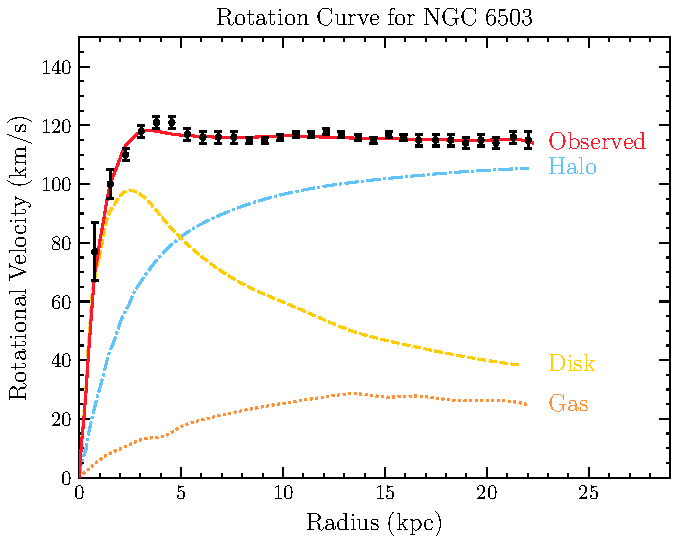
\includegraphics{gal_rotn_N6503}
    \caption{Galaxy rotation curve for NGC 6503, showing the contributions to the total velocity (red) from the DM halo (blue), disk (yellow), and gas components. Data used in making this plot was obtained from~\cite{Freese:2008cz_may_ReviewObservationalEvidence, Lelli:2016zqa_SPARCMassModels}.}
    \label{ch1:fig:gal_rotn_curve}
\end{figure}

\subsubsection*{Gravitational Lensing}

As described by General Relativity, the curvature of space-time around massive entities causes light to travel along curved paths. 
As such, the mass of astrophysical structures can be deduced from the extent to which they distort the images of objects in the background. The extent of the distortions depends on how massive the foreground object is, ranging from the shearing of the background image (weak lensing), to multiple copies of the background object appearing (strong lensing)~\cite{Schneider_Gravitationallensingstrong}.  The disparity between the mass obtained from gravitational lensing and the mass of visible matter in the system is further evidence of dark matter's existence~\cite{SDSS:2005sxd_FourthDataRelease, Mandelbaum:2005nx_Galaxyhalomasses}. 

\subsubsection*{The Bullet Cluster}
Galaxy cluster 1E 0657-56, commonly referred to as the ``bullet cluster'', was formed by the collision of two separate galaxy clusters. 
The baryonic matter in these clusters is mostly composed of a strongly interacting gas and, as expected, produced a significant amount of X-rays during the collision. These X-rays were imaged by the Chandra X-Ray telescope~\cite{Clowe:2003tk_Weaklensingmass}, providing information on the resulting distribution of the visible matter. This is shown by the red regions of Fig.~\ref{ch1:fig:bullet_cluster}, where it can be seen how the visible matter has been smeared due to the collision. 
However, when the gravitational potential was mapped using gravitational lensing, it was clear that the majority of the mass was displaced relative to the visible matter. This mass is attributed to the dark matter components of the original clusters. As indicated by the purple regions in Fig.~\ref{ch1:fig:bullet_cluster}, the dark matter halos seem to have passed through each other mostly unperturbed. This tells us that not only is the majority of the mass comprised of dark matter, but that the dark matter has extremely weak interactions with both the visible matter and itself. 

\begin{figure}[t!bp]
    \centering
    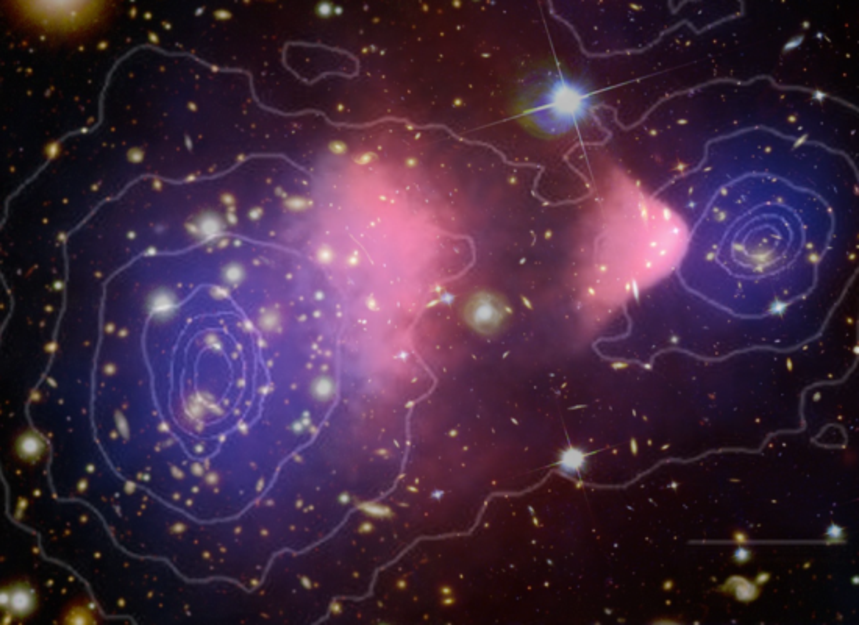
\includegraphics[width = 0.75\textwidth]{bullet_cluster}
    \caption{Image of the Bullet Cluster with contours of the gravitational potential superposed. The red regions indicate the baryonic matter after the collision, while the purple regions are the expected DM components deduced from gravitational lensing. \cite{Clowe:2003tk_Weaklensingmass,Randall:2008ppe_ConstraintsSelfInteractionCrossSection}}
    \label{ch1:fig:bullet_cluster}
\end{figure}

%%%%%%%%%%%%%%%%%%%%%%%%%%%%%%%%%%%%%
%%%%%%%%%%%%%%%%%%%%%%%%%%%%%%%%%%%%%
\subsection{Cosmological Evidence}
\label{ch1:subsec:cosmo_evidence}
%%%%%%%%%%%%%%%%%%%%%%%%%%%%%%%%%%%%%
%%%%%%%%%%%%%%%%%%%%%%%%%%%%%%%%%%%%%
 
The current best cosmological model is the $\Lambda$-Cold Dark Matter model ($\Lambda$CDM), in which $\Lambda$ refers to the cosmological constant associated with dark energy, and as the name suggests, cold (i.e. non-relativistic) dark matter plays a prominent role. The key components of this model are the aforementioned dark energy and dark matter, along with baryonic matter, and it assumes that gravity is described by Einstein's General Relativity. The total energy density of the universe, $\rho_\mathrm{Univ.}$, can be broken down into three components based on how their density redshifts with the expansion of the Universe. In the $\Lambda$CDM model, these components are matter, radiation, and the vacuum energy $\Lambda$. The cosmological abundances of each component, ($\Omega_\mathrm{m}$, $\Omega_\mathrm{r}$, $\Omega_\Lambda$ respectively), are expressed as a fraction of the critical density, $\rho_\mathrm{crit}$,     
\begin{align}
    \rho_\mathrm{crit}   & = \frac{H^2}{8 \pi G_N},\\
    \Omega_i & = \frac{\rho_i}{\rho_\mathrm{crit}},
\end{align}
where $H$ is the Hubble parameter, such that the total energy density of the Universe satisfies
\begin{equation}
    \Omega_\mathrm{m} + \Omega_\mathrm{r} + \Omega_\Lambda = \frac{\rho_\mathrm{Univ.}}{\rho_\mathrm{crit}}.
\end{equation}
The ratio $\rho_\mathrm{Univ.}/\rho_\mathrm{crit}$ determines the curvature of the universe, with values greater than 1 corresponding to a closed universe, less than 1 to an open universe, and equal to 1 to a spatially flat universe. Current observations are consistent with a spatially flat universe, and so we have $\sum_i \Omega_i = 1$.


The $\Lambda$CDM model has seen huge success as it provides explanations for observed the power spectrum of the Cosmic Microwave Background (CMB), the large-scale structure of the Universe, the abundances of light elements (hydrogen, deuterium, helium, and lithium), and the accelerated expansion rate of the Universe. These observations constrain the parameters of the model and hence provide a complimentary probe of the properties of dark matter to the astronomical observations discussed above.

\subsubsection*{The Cosmic Microwave Background}
One of the strongest probes of cosmological models is the Cosmic Microwave Background (CMB), relic photons from the time epoch of last scattering. This occurred after recombination, at a temperature of around $\sim 3000 \K$, once the photons had decoupled from the baryonic matter and could freely propagate through the universe. The photons observed today have been redshifted by the expansion of the Universe and are well described by a blackbody spectrum with a temperature of $T_\mathrm{CMB} = 2.73\pm 0.0006\K$. Observations of the CMB temperature reveal that it is not exactly isotropic, with anisotropies at the level of $\delta T_\mathrm{CMB}/T_\mathrm{CMB}\sim 10^{-5} - 10^{-6} $ seen on a range of angular scales in the sky. These anisotropies were seeded by the primordial density perturbations that arise during inflation. These perturbations evolve due to the acoustic oscillations of the photon-baryon plasma driven by the interplay between the pressure from the photons and the gravitational attraction of the matter. The oscillations cease once the photons decouple, freezing in their temporal phases that are observed as peaks in the angular power spectrum of the temperature anisotropies. 

Measurements of the CMB power spectrum provide information on many of the cosmological parameters. The locations of the acoustic peaks depend on the spatial geometry of the Universe and hence constrains $\Omega_\mathrm{tot}$. The total matter density, $\Omega_\mathrm{m}$, affects how the CMB spectrum is gravitationally lensed.  The relative amplitudes of the peaks probe the baryon-to-photon ratio and hence the baryon density, $\Omega_\mathrm{b}$. Finally, the density of dark matter, $\Omega_\mathrm{DM}$, is obtained by fitting the cosmological parameters to the exact shape of the spectrum~\cite{Freese:2008cz_may_ReviewObservationalEvidence, Planck:2018vyg_sep_Planck2018results}. 

The Planck collaboration most recently performed a precise measurement of the CMB power spectrum in 2018, obtaining best-fit parameters~\cite{Planck:2018vyg_sep_Planck2018results,Planck:2019nip_sep_Planck2018results}
\begin{equation}
     \Omega_\mathrm{m} = 0.311 \pm 0.006,\quad \Omega_\Lambda = 0.689 \pm 0.006,
\end{equation}
for the matter and dark energy densities. They obtained a total energy density of $\Omega_\mathrm{tot} = 1.011 \pm 0.006$ at $68\%$ confidence level, providing strong evidence for a spatially flat Universe. 
The breakdown of the matter density into the dark and baryonic components is determined by combining the CMB results with constraints from Big Bang Nucleosynthesis (BBN)\footnote{BBN is the process that produced the light elements (D, $\ce{^3 He}$, $\ce{^4 He}$, and $\ce{^7 Li}$) were produced in the early universe. This process is highly sensitive to the physical condition of the universe at that time, allowing for strong constraints to be placed on physics beyond the Standard Model.} giving
\begin{equation}
    \Omega_\mathrm{DM}h^2 = 0.1193 \pm 0.0009,\quad \Omega_\mathrm{b}h^2 = 0.02242 \pm 0.00014,
\end{equation}
where $h$ is the dimensionless Hubble constant such that the Hubble parameter today is $H_0 = 100\, h\km\s^{-1}\;\mathrm{Mpc}$. 

% The result for the baryon density is consistent with the value obtained from Big Bang Nucleosynthesis (BBN), the process in which light elements are formed in the early universe. BBN gives a baryon density of $\Omega_\mathrm{b} = 0.0220 \pm 0.0004$, in good agreement with the CMB result.


\subsubsection*{Large Scale Structure}
After recombination, the pressure on the baryonic matter from photons began to decrease, eventually allowing the small density perturbations to grow. This led to the growth of stars, galaxies, and the large-scale structure we observe today~\cite{Springel:2006vs_LargescalestructureUniverse}. N-body simulations of the Universe's evolution require a cold dark matter component for this structure to form. While a small component of the dark matter can be warm, hot dark matter would wash out small-scale structures~\cite{Springel:2005nw_Simulatingjointevolution}.  

%%%%%%%%%%%%%%%%%%%%%%%%%%%%%%%%%%%%%
%%%%%%%%%%%%%%%%%%%%%%%%%%%%%%%%%%%%%
%%%%%%%%%%%%%%%%%%%%%%%%%%%%%%%%%%%%%
\section{Potential Models of Dark Matter}
\label{ch1:sec:DM_models}
%%%%%%%%%%%%%%%%%%%%%%%%%%%%%%%%%%%%%
%%%%%%%%%%%%%%%%%%%%%%%%%%%%%%%%%%%%%
%%%%%%%%%%%%%%%%%%%%%%%%%%%%%%%%%%%%%

Given that baryonic matter is composed of particles described by the Standard Model (SM) of particle physics, it is a fair assumption that dark matter will also have a particle nature. Therefore, models of particle dark matter are built by extending the SM in a way consistent with its symmetries. 
Such models may be as simple as introducing a single new field into the SM, or there may be a more extensive hidden sector with a complicated symmetry structure. Additionally, there are compelling theories in which dark matter is not a fundamental particle, such as primordial black holes (PBHs) formed in the early universe. Given the few details we know about dark matter, there exists an enormous library of viable dark matter candidates. However, there are generic properties a good dark matter candidate must satisfy, namely:
\begin{itemize}
    \item \textbf{Stable on Cosmological Timescales:} Dark matter must either be stable or have a lifetime significantly longer than the age of the Universe to be present in its current abundance. 
    
    \item \textbf{Neutral or milli-charged under Electromagnetism:} Dark matter, as its name suggests, does not significantly interact with light. Requiring that dark matter be completely decoupled from the Standard Model plasma by the time of recombination yields an upper bound on the electric charge of dark matter~\cite{McDermott:2010pa_TurningLightsHow} 
    \begin{equation}
        q_\mathrm{DM}/e < \begin{cases}
            3.5\times10^{-7} \left( \frac{m_\mathrm{DM}}{1\GeV}\right)^{0.58},\quad m_\mathrm{DM} > 1\GeV\\
            4.0\times 10^{-7}\left( \frac{m_\mathrm{DM}}{1\GeV}\right)^{0.35},\quad m_\mathrm{DM} <1\GeV
        \end{cases}
    \end{equation}
    
    \item \textbf{Small Self-Interactions:} The standard $\Lambda$CDM cosmology assumes that the dark matter is collisionless. However, small dark matter self-interactions can help resolve existing small-scale structure issues~\cite{Tulin:2017ara_feb_DarkMatterSelfinteractions, Spergel:1999mh_Observationalevidenceselfinteracting}. Current limits on the self-interaction cross-section are $\sigma_{\mathrm{DM-DM}}/m_\mathrm{DM} < 0.48\cm^2/\mathrm{g}$ come from merging galaxy clusters~\cite{Randall:2008ppe_ConstraintsSelfInteractionCrossSection} and the ellipticity of galaxies obtained from X-ray observations~\cite{Buote:2002wd_ChandraEvidenceFlattened}.

    \item \textbf{Cold:} Dark matter is required to be non-relativistic at the time of structure formation. At most, a small component of the dark matter can be warm (semi-relativistic).
\end{itemize}
A selection of the more prominent dark matter candidates is shown in Fig.~\ref{ch1:fig:DM_models_landscape}. The key features of a few of these models are discussed below.

%%%%%%%%%%%%%%%%%%%%%%%%%%%%%%%%%%%%%%%%%
\begin{figure}[t!]
    \centering
    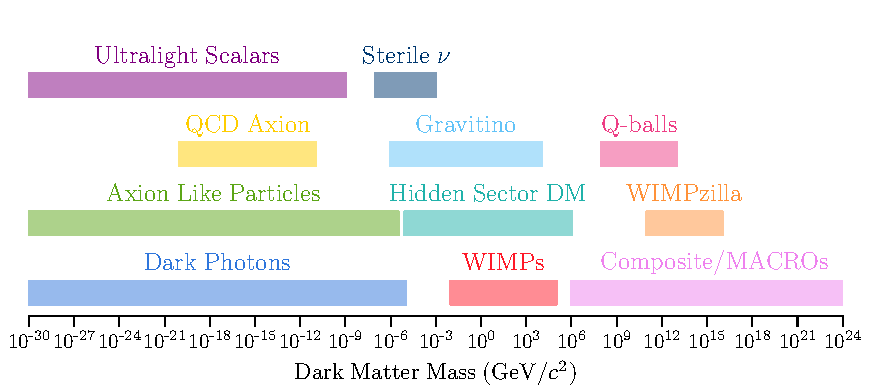
\includegraphics{DM_model_landscape}
    \caption{Illustrative landscape of dark matter models and the mass range for which they predict a valid candidate. Details can be found in the Dark Matter chapter of the PDG~\cite{ParticleDataGroup:2022pth_aug_ReviewParticlePhysics}.}
    \label{ch1:fig:DM_models_landscape}
\end{figure}
%%%%%%%%%%%%%%%%%%%%%%%%%%%%%%%%%%%%%%%%%

\subsubsection*{WIMPs}
Weakly Interacting Massive Particles (WIMPs) are a class of dark matter candidates that generically have masses and interaction strengths around the weak scale. Many extensions of the SM naturally predict the existence of such a particle, with famous examples being the lightest supersymmetric particle in supersymmetric theories~\cite{Goldberg:1983nd_ConstraintPhotinoMass}, or the lightest stable Kaluza-Klein mode in theories with extra dimensions~\cite{Kolb:1983fm_DimensionalReductionEarly}. 

Nowadays, WIMP dark matter is used almost synonymously to mean thermal relic, referring to a species whose relic abundance is produced thermally in the early universe through the freeze-out mechanism~\cite{Jungman:1995df_Supersymmetricdarkmatter}.
In this paradigm, the WIMP is initially in thermal equilibrium with the Standard Model bath. This equilibrium is maintained as long as the interaction rates of the WIMP with the bath, denoted $\Gamma$, remain faster than the Hubble expansion of the universe, $H$. As the universe continues to expand, the temperature of the bath drops, slowing down the interaction rates. Eventually, the expansion rate overtakes the interaction rates, $\Gamma/H\lesssim 1$, and the interactions ``freeze out'' causing the WIMP to fall out of equilibrium with the bath. At this point, the WIMPs can no longer efficiently annihilate, and their abundance gets ``frozen-in'' to the value it had at freeze-out, leading to the abundance observed today. 


A cold thermal relic, such as dark matter, will freeze out after it has become non-relativistic. In this scenario, the interaction rates become Boltzmann suppressed\footnote{The number density of a non-relativistic species in thermal equilibrium with the bath will follow $n \propto \left(m T_\mathrm{bath}\right)^{3/2} \exp\left(-m /T_\mathrm{bath}\right)$. Once the temperature falls below the mass of the species, the number density becomes exponentially suppressed. This is what is known as ``Boltzmann suppression''.}, and the species rapidly freezes out. The relic density is therefore sensitive to the annihilation cross-section of the species, $\langle \sigma_\mathrm{ann} v\rangle$. More efficient annihilations correspond to larger cross-sections, resulting in the species remaining in equilibrium for longer times. This allows the number density to continue following the exponentially decreasing Boltzmann distribution and yield a smaller relic abundance. The evolution of the abundance of a Majorana fermion WIMP of mass $m_\mathrm{WIMP} = 100\GeV$ is shown in Fig.~\ref{ch1:fig:WIMP_freezeout} for three values of the annihilation cross-section. A simple expression  relating the annihilation cross-section and the abundance that is correct to $\sim5\%$ can be obtained~\cite{Steigman:2012nb_PreciseRelicWIMP} 
\begin{align}
    \Omega_{\mathrm{DM}}h^2 & = \frac{10^{-27}\cm^3\s^{-1}}{\sigmav} \frac{x_*}{g_*^{1/2}}\\
     &\sim 0.12 \; \left(\frac{2.2\times 10^{-26}\cm^3 \s^{-1}}{\langle \sigma v\rangle}\right),\quad m_\chi\gtrsim 10\GeV,
\end{align}
where $x_* = m_\mathrm{WIMP}/T_*$ is evaluated at an intermediate temperature between equilibrium and freeze-out, with $g_*$ the effective number of relativistic degrees of freedom present at this time. 

\begin{figure}[t!]
    \centering
    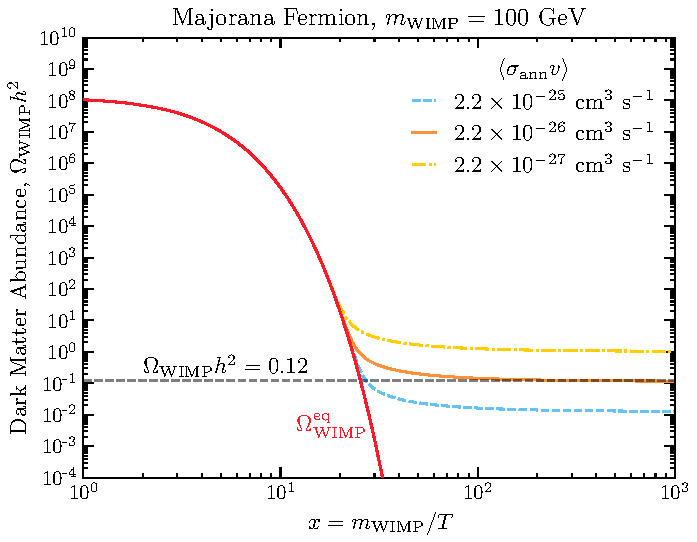
\includegraphics{fig_dm_freezeout.pdf}
    \caption{Evolution of the DM abundance as a function of $x = m_\mathrm{DM}/T$. The red line tracks the abundance of the WIMP if it remains in equilibrium with the bath. The relic abundance for three different annihilation cross-sections is shown in blue, orange, and yellow for $\langle \sigma_\mathrm{ann} v\rangle = 2.2\times10^{-25},\;2.2\times10^{-26},$ and $2.2\times10^{-27}$ cm$^{3}$s$^{-1}$ respectively.}
    \label{ch1:fig:WIMP_freezeout}
\end{figure}

The allowed mass range for a thermal WIMP is between $10\MeV\lesssim m_\mathrm{WIMP} \lesssim 100\TeV$. Lighter WIMPs will make non-negligible contributions to the effective number of neutrinos at the time of Big Bang Nucleosynthesis, measured to be $N^\mathrm{BBN}_{eff} = 3.044$~\cite{Yeh:2022heq_oct_Probingphysicsstandard}, altering the observed abundances of the light elements. The CMB offers an additional probe of $N_\mathrm{eff}$ at the later time of recombination and can be combined with the BBN result leading to the value $N_{eff} = 2.99 \pm 0.17$~\cite{Planck:2018vyg_sep_Planck2018results}. Given the Standard Model predicts a value of $N_\mathrm{eff} = 3.044$, contributions from additional relativistic degrees of freedom must be less than $\Delta N_\mathrm{eff} < 0.28$~\cite{Yeh:2022heq_oct_Probingphysicsstandard}.  
At the high end of this range, masses larger than $\sim 100\TeV$ are excluded from partial wave unitarity~\cite{Griest:1989wd_UnitarityLimitsMass}. 
 

\subsubsection{Axions}
The axion originally arose from the Pecci-Quinn solution to the Strong CP problem. This refers to the lack of observed CP-violation in the QCD sector of the Standard Model that arises from the topological term in the Lagrangian
\begin{equation}
    \mathcal{L}_{\theta_\mathrm{QCD}} = \frac{g_s^2}{32 \pi}\theta_\mathrm{QCD} G_{\mu\nu} \tilde{G}^{\mu\nu},
\end{equation}
where $g_s$ is the QCD coupling constant, $G_{\mu\nu}$ is the gluon field strength tensor and $\tilde{G}^{\mu\nu}$ is its dual. This term generates an electric dipole moment for the neutron (nEDM) that has yet to be observed experimentally. The current upper bound on the nEDM is $|d_n| < 0.18\times 10^{-26}\;e\cm$~\cite{Abel:2020pzs_feb_MeasurementPermanentElectric} and can be translated to an upper bound on the CP-violating QCD $\theta$-parameter such that $|\theta_{QCD}|\lesssim 10^{-10}$, raising questions as to why this value seems to be fine-tuned to such a small value. 

The Peccei-Quinn solution to this problem introduces a new, anomalous, global  $U(1)_{\mathrm{PQ}}$ symmetry and promotes $\theta_\mathrm{QCD}$ to be a dynamical field.
Wilczck~\cite{Wilczek:1977pj_ProblemStrongInvariance} and Weinberg~\cite{Weinberg:1977ma_NewLightBoson} showed that the axion emerges as the pseudo-Goldstone boson associated with the breaking of $U(1)_\mathrm{PQ}$. Though the original axion was quickly out, many modern extensions of the SM predict the existence of a QCD axion. Two of the most prominent UV completions of the axion are the KSVZ~\cite{Kim:1979if_WeakInteractionSinglet, Shifman:1979if_CanConfinementEnsure} and DFSZ~\cite{_PossibleSuppressionAxion, Dine:1981rt_SimpleSolutionStrong} models. In these models, the axion produced in the early Universe can serve the role of cold dark matter today. This makes it a very compelling dark matter candidate, as it solves two of the biggest mysteries of physics in one neat package. 

However, solving the Strong CP problem can be rather restrictive on the model parameters. For example, the QCD axion's coupling to the photon, $g_{a\gamma\gamma}$, is not a free parameter and depends on the scale at which the PQ symmetry is broken. Many models introduce a light pseudoscalar particle, say $a$, that couples to the photon in the same way as the QCD axion,  
\begin{equation}
    \mathcal{L}_{a\gamma\gamma} = -\frac{g_{a\gamma\gamma}}{4} a F_{\mu\nu}\tilde{F}^{\mu\nu},
\end{equation}
but is not associated with a solution to the Strong CP problem. Such pseudoscalars are known as ``Axion Like Particles" (ALPs) and can make a good dark matter candidate.

\subsubsection*{Primordial Black Holes}

Primordial black holes (PBHs) are formed during the early Universe through various mechanisms. The simplest mechanism predicts that PBHs are produced from the gravitational collapse of superhorizon density fluctuations seeded during inflation~\cite{Hawking:1971ei_apr_Gravitationallycollapsedobjects, Carr:1974nx_Blackholesearly,Carr:1975qj_Primordialblackhole}. 
Unlike black holes that originate from stellar collapse, which have masses $\gtrsim 3\Msun$, the mass of a PBH can be arbitrary.  PBHs can also make a good dark matter candidate, satisfying all the criteria points outlined above. In fact, PBHs with a mass between $\sim (10^{-17} - 10^{-12})\;\Msun$, dubbed ``asteroid mass PBHs'', can account for 100\% of the dark matter content in the Universe~\cite{Montero-Camacho:2019jte_aug_Revisitingconstraintsasteroidmass}. Outside this range, PBHs can still make up a small fraction of dark matter~\cite{Villanueva-Domingo:2021spv_may_Briefreviewprimordial}. 
% As opposed to the WIMPs and ALPs above, PBHs are macroscopic objects, that is, they are not themselves fundamental particles. 

%%%%%%%%%%%%%%%%%%%%%%%%%%%%%%%%%%%%%
%%%%%%%%%%%%%%%%%%%%%%%%%%%%%%%%%%%%%
\subsection{Dark Matter in an Effective Field Theory Framework}
\label{ch1:subsec:DM_EFTs}
%%%%%%%%%%%%%%%%%%%%%%%%%%%%%%%%%%%%%
%%%%%%%%%%%%%%%%%%%%%%%%%%%%%%%%%%%%%

For a dark matter candidate to be truly compelling, it should be able to be embedded into an ultraviolet (UV) complete theory. Such theories are renormalisable\footnote{In a renormalisable theory, the infinities that arise from UV divergences can be absorbed by fixing a finite number of parameters to experimentally observed values.} and gauge invariant under the SM gauge group $SU(3)_\mathrm{colour}\otimes SU(2)_L\otimes U(1)_Y$. This allows them to be predictive up to arbitrarily high energies. These theories are typically quite complex, requiring the introduction of multiple new fields and many more free parameters. As an example, consider the phenomenological Minimal Supersymmetric Standard Model (pMSSM)~\cite{Villanueva-Domingo:2021spv_may_Briefreviewprimordial} in which the lightest neutralino\footnote{The neutralinos are the mass eigenstates of the supersymmetric partners of the neutral gauge bosons and the higgsino.} can be a thermal WIMP dark matter candidate. In this theory, 19 free parameters are introduced on top of the free parameters in the SM, requiring 38 independent experimental observations to fully constrain the model. Given that at this time, all good dark matter candidates are equally likely to be the correct one, a model-independent approach to interpreting experimental results is desirable. This is achieved by describing the interactions of dark matter with the SM through an effective field theory (EFT).

%%%%%%%%%%%%%%%%%%%%%%%%%%%%%%%%%%%%%
\subsection{Overview of Effective Field Theory}
\label{ch1:subsec:EFT_intro}
%%%%%%%%%%%%%%%%%%%%%%%%%%%%%%%%%%%%%

Modern physics can be thought of as a ladder of theories that are designed to describe the physics present at a given energy (or length) scale. For example, Newtonian mechanics is a sufficient description of the physics experienced in our everyday lives. However, in situations where the energy is comparable to the mass of the system, Newtonian mechanics breaks down, and Special Relativity must be used to describe the physics. In particle physics, the Standard Model provides an excellent description of particle interactions up to the energies reached at LHC, 13.6$\TeV$, and perhaps even further beyond. However, even it is expected to break down at higher energy scales, in particular at the Planck scale, where a quantum theory of gravity is required. Hence, both Newtonian mechanics and the SM are low-energy, effective descriptions of a more complete theory.

This philosophy based on only describing the physics relevant below some energy scale, $\Lambda$, is the core principle of EFTs. The Lagrangian for the effective theory only contains the degrees of freedom that can be produced below the scale $\Lambda$, i.e. fields that have masses less than this scale. This low-energy regime described by the EFT is often called the infrared (IR) regime. 

In general, the EFT Lagrangian will contain renormalizable terms, $\mathcal{L}_\mathrm{renorm.}$,  built out of operators that have mass dimension $\leq 4$, as well as operators with mass dimension $n> 4$, $\mathcal{O}_i^{(n)}$, that encapsulate the contributions from the UV physics. Each of these higher dimensional operators will be suppressed by the scale of new physics, $\Lambda^{4-n}$. 
The effective Lagrangian can then be written as
\begin{equation}
    \mathcal{L}_\mathrm{EFT} = \mathcal{L}_\mathrm{renorm.} +  \sum_{n>4}   \sum_{i = 1}^{j_n} \frac{C_i^{(n)} (\tilde{\mu})}{\Lambda^{n-4}}\mathcal{O}_i^{(n)},
    \label{ch1:eq:EFT_Lagrangian}
\end{equation}
where we sum over all $j_n$ operators present at mass dimension $n$. The expansion coefficients, $C_i^{(n)}$, are the Wilson coefficients that contain the effects of the UV physics. In general, the Wilson coefficients run with the energy scale they are evaluated at, $\tilde{\mu}$, described by the renormalisation group equations (RGEs).
The sum over the mass dimension of the operators is typically terminated at some sensible value, as higher dimensional operators get increasingly suppressed by the cutoff scale $\Lambda$.

The series of operators in Eq.~\ref{ch1:eq:EFT_Lagrangian} can be constructed in two different ways. First, we assume some prior knowledge of the underlying UV theory. Then, for a given energy scale $\Lambda$, the heavy degrees of freedom are known, and can be explicitly integrated out. There are various methods for performing this process, the simplest being expanding the propagator of the heavy fields in powers of the momenta over the heavy mass, $(p/M)^2$. For the simple case of a heavy scalar, this corresponds to 
\begin{equation}
    \frac{i}{p^2 - M^2} = \frac{-i}{M^2}\left(\frac{1}{1 - (p/M)^2}\right)\approx \frac{-i}{M^2}\left( 1 + \left(\frac{p}{M}\right)^2 + \mathcal{O}\left(\left(\frac{p}{M}\right)^4\right)\right).
\end{equation}
An alternate method is to replace the heavy fields in the Lagrangian with their classical equations of motion. The resulting effective Lagrangian will contain all the operators generated by the UV theory at tree level.
Constructing an EFT in this way is called the \textit{top-down} method.

The second method of constructing an EFT is to be agnostic to the UV physics and write down all possible operators that can be constructed from the IR degrees of freedom. These operators must obey the symmetries of the IR theory, as well as any other constraints one wishes to impose\footnote{For example, one might require that no flavour changing processes are present at dimension 5, despite such operator being allowed by the symmetries.}. This is the \textit{bottom-up} approach, offering a more model-independent approach than the top-down method. The Wilson coefficients, in this case, will be arbitrary functions of the energy scale determined by solving the RGEs.

In general, the parameter space of the EFT will be lower dimensional than those of the corresponding UV models. This allows for an easier comparison with experimental results, as fewer parameters need to be fit to the data. Once the Wilson coefficients have been constrained at the low energy scale of the experiments, they can be matched to the coefficients generated by some UV theory at another scale, thereby constraining the UV parameters. 

\subsection{Dimension 6 EFT Operators for Dirac Fermion Dark Matter}
This work will focus on dimension 6 EFT operators that describe the interactions of Dirac fermion dark matter with standard model fermions. These operators will have a structure 
\begin{equation}
    \mathcal{L}_\mathrm{EFT}^{(6)} \sim \frac{1}{\Lambda^2}(\bar{\chi}\Gamma_\mathrm{DM} \chi)(\bar{f}\Gamma_{\mathrm{SM}}f),
\end{equation}
where the $\Gamma_i$ determines the Lorentz structure of the interaction by taking appropriate combinations from the set
\begin{equation}
    \Gamma_i\in \{1, i\gamma_5, \gamma^\mu, i\gamma^\mu \gamma^5, \sigma^{\mu\nu}, i \sigma^{\mu\nu}\gamma^5\}.
\end{equation}
For example, the case of $\Gamma_\chi = \Gamma_\mathrm{SM} = 1$ yields scalar currents for both the DM and SM fermions and would correspond to integrating out a heavy scalar mediator in the UV theory. Under the assumption of minimal flavour violation (MFV)\footnote{MFV is the assumption that the only source of flavour violation in the quark sector comes from the SM Yukawa matrices and not from any new physics introduced at a higher scale.} are ten such operators at dimension six that form a linearly independent basis. These are given in Table~\ref{ch1:tab:opers_defn_full}, along with spin-averaged squared matrix element for dark matter scattering with a fermion. 
The operators are classified based on the Lorentz nature of the SM fermion bilinear; D1-2: Scalar (S), D3-4: Pseudoscalar (P), D5-6: Vector (V), D7-8: Axial-vector (A), and D9-10: tensor (T).
The coupling constant, $g_f$, for operators that involve the S and P fermion bilinears (operators D1-4) are normalised by the corresponding Yukawa couplings. This is because, in a UV complete theory, these bilinears would couple to the new scalar/pseudoscalar field that mediates the interactions with the dark matter. In many models, this new field will mix with the SM Higgs field, leading to couplings that depend on the fermion masses. The remaining bilinears have coupling constants that depend only on the cutoff scale, $\Lambda_f$.


\begin{table}[t!bp]
\centering
\setlength{\tabcolsep}{0.25em}   
\begin{tabular}{  c  c  c  c  c }
\toprule
  Name & Operator & $g_f$  & $|\overline{M}(s,t,m_i)|^2$   \\\midrule\midrule
  D1 & $\bar\chi  \chi\;\bar f  f $ & $\frac{y_f}{\Lambda_f^2}$  & $ g_f^2\frac{\left(4 m_{\chi }^2-t\right) \left(4 m_{\chi }^2-\mu ^2   t\right)}{\mu ^2}$ \\  
  D2 & $\bar\chi \gamma^5 \chi\;\bar f f $ & $i\frac{y_f}{\Lambda_f^2}$ & $g_f^2\frac{t \left(\mu ^2 t-4 m_{\chi }^2\right)}{\mu ^2}$ \\  
  D3 & $\bar\chi \chi\;\bar f \gamma^5  f $&  $i\frac{y_f}{\Lambda_f^2}$  &  $g_f^2 t \left(t-4 m_{\chi }^2\right)$ \\ 
  D4 & $\bar\chi \gamma^5 \chi\; \bar f \gamma^5 f $ & $\frac{y_f}{\Lambda_f^2}$  & $g_f^2 t^2$  \\
  D5 & $\bar \chi \gamma_\mu \chi\; \bar f \gamma^\mu f$ & $\frac{1}{\Lambda_f^2}$ &  $2 g_f^2 \frac{2 \left(\mu ^2+1\right)^2 m_{\chi }^4-4 \left(\mu ^2+1\right) \mu ^2 s m_{\chi }^2+\mu ^4 \left(2 s^2+2 s t+t^2\right)}{\mu^4}$ \\ 
  D6 & $\bar\chi \gamma_\mu \gamma^5 \chi\; \bar  f \gamma^\mu f $ & $\frac{1}{\Lambda_f^2}$ & $2  g_f^2\frac{2 \left(\mu ^2-1\right)^2 m_{\chi }^4-4 \mu ^2 m_{\chi }^2 \left(\mu ^2 s+s+\mu ^2 t\right)+\mu ^4 \left(2 s^2+2 s   t+t^2\right)}{\mu^4}$ \\ 
  D7 & $\bar \chi \gamma_\mu  \chi\; \bar f \gamma^\mu\gamma^5  f$ & $\frac{1}{\Lambda_f^2}$ &  $2  g_f^2 \frac{2 \left(\mu ^2-1\right)^2 m_{\chi }^4-4 \mu ^2 m_{\chi }^2 \left(\mu ^2 s+s+t\right)+\mu ^4 \left(2 s^2+2 s t+t^2\right)}{\mu^4}$ \\  \
  D8 & $\bar \chi \gamma_\mu \gamma^5 \chi\; \bar f \gamma^\mu \gamma^5 f $ & $\frac{1}{\Lambda_f^2}$ & $2  g_f^2 \frac{2 \left(\mu ^4+10 \mu ^2+1\right) m_{\chi }^4-4 \left(\mu ^2+1\right) \mu ^2  m_{\chi }^2 (s+t)+\mu ^4 \left(2 s^2+2 s t+t^2\right)}{\mu ^4}$ \\  
  D9 & $\bar \chi \sigma_{\mu\nu} \chi\; \bar f \sigma^{\mu\nu} f $ & $\frac{1}{\Lambda_f^2}$ & $8  g_f^2 \frac{4 \left(\mu ^4+4 \mu ^2+1\right) m_{\chi }^4-2 \left(\mu ^2+1\right) \mu ^2 m_{\chi  }^2 (4 s+t)+\mu ^4 (2 s+t)^2}{\mu ^4}$ \\  
 D10 & $\bar \chi \sigma_{\mu\nu} \gamma^5\chi\; \bar f \sigma^{\mu\nu} f $ & $\frac{i}{\Lambda_f^2}$ &  $8  g_f^2\frac{4 \left(\mu ^2-1\right)^2 m_{\chi }^4-2 \left(\mu ^2+1\right) \mu ^2 m_{\chi }^2 (4 s+t)+\mu ^4 (2 s+t)^2}{\mu^4}$\\  \bottomrule
\end{tabular}
\caption{Dimension 6 EFT operators~\cite{Goodman:2010ku_ConstraintsDarkMatter} for the coupling of Dirac DM to fermions (column 2), together with the squared matrix elements DM-fermion scattering (column 5), where $s$ and $t$ are Mandelstam variables, $\mu=m_\chi/m_T$, and $m_T$ is the target mass. 
\label{ch1:tab:opers_defn_full} }
\end{table}

\subsection{From DM-Quark to DM-Nucleon Interactions}
\label{ch1:subsec:quark_to_nucleon_EFT}

The operators in Table~\ref{ch1:tab:opers_defn_full} describe dark matter interactions at the quark level, as these are the degrees of freedom most models are formulated with. However, we will primarily be interested in dark matter scattering with baryons, which requires taking the matrix element of the quark operators between baryon states, i.e. $\langle {\cal B} | \bar q \, \Gamma_q q| {\cal B}\rangle$. These matrix elements can be calculated through the application of Chiral Perturbation Theory (ChPT), giving a baryon level EFT. The operators of this EFT will have the same form as those in Table~\ref{ch1:tab:opers_defn_full}, with the obvious replacement of $f\rightarrow \cal B$, as well as additional form factors that take into account the structure of the baryons.

The required form factors for each operator have been calculated at zero momentum transfer in Ref.~\cite{Cirelli:2013ufw_oct_Toolsmodelindependentbounds} and are given by 
\begin{align}
c_{\cal B}^S(0) &= \frac{2 m_{\cal B}^2}{v^2}\left[\sum_{q=u,d,s}f_{T_q}^{(\cal B)}+\frac{2}{9}f_{T_G}^{(\cal B)}\right]^2,\label{ch1:eq:cBS}\\
c_{\cal B}^P(0) &= \frac{2 m_{\cal B}^2}{v^2}\left[\sum_{q=u,d,s}\left(1-3\frac{\overline{m}}{m_q}\right)\Delta_q^{(\cal B)}\right]^2,\label{ch1:eq:cBP}\\
c_{\cal B}^V(0) &= 9,\label{ch1:eq:cBV}\\
c_{\cal B}^A(0) &=  \left[\sum_{q=u,d,s}\Delta_q^{(\cal B)}\right]^2,\label{ch1:eq:cBA}\\
c_{\cal B}^T(0) &= \left[\sum_{q=u,d,s}\delta_q^{(\cal B)}\right]^2,\label{ch1:eq:cBT}
\end{align}
where  $v=246$ GeV is the vacuum expectation value of the SM Higgs field, $\cal B$ is the baryonic species,  $\overline{m}\equiv(1/m_u+1/m_d+1/m_s)^{-1}$ and $f_{T_q}^{(\cal B)}$, $f_{T_G}^{(\cal B)}=1-\sum_{q=u,d,s} f_{T_q}^{(\cal B)}$, $\Delta_q^{(\cal B)}$ and $\delta_q^{(\cal B)}$ are the hadronic matrix elements, determined either experimentally or by lattice QCD simulations. The specific values of these matrix elements for various baryons are provided in Appendix~\ref{app:hadronic_matrix_elements}.

The assumption of zero-momentum transfer is valid when considering interactions with momentum transfers $\lesssim 1\GeV$, such as in direct detection experiments. Once the momentum transfer exceeds this, the internal structure of the baryon begins to be resolved, and an additional momentum-dependent form factor is required to account for this~\cite{_ElectromagneticStructureNucleon},
\begin{equation}
    F_{\cal B}(t) = \frac{1}{\left( 1 - t/Q_0\right)^2},
\end{equation}
where $t$ is the Mandelstam variable, and $Q_0$ is an energy scale that depends on the hadronic form factor. For simplicity, we will conservatively take $Q_0 = 1 \GeV$ for all operators.
Putting everything together, the squared coupling constants for dark matter-baryon interactions are obtained by making the replacement
\begin{equation}
    g_f^2 \rightarrow \frac{c^I_{\cal B}(t)}{\Lambda_q^4} \equiv \frac{1}{\Lambda_q^4}c_{\cal B}^I(0)F^2_{\cal B}(t),\quad I\in {S, P, V, A, T},
\end{equation}
in the matrix elements in the final column of Table~\ref{ch1:tab:opers_defn_full}.



%%%%%%%%%%%%%%%%%%%%%%%%%%%%%%%%%%%%%
%%%%%%%%%%%%%%%%%%%%%%%%%%%%%%%%%%%%%
%%%%%%%%%%%%%%%%%%%%%%%%%%%%%%%%%%%%%
\section{Current Status of Dark Matter Constraints}
%%%%%%%%%%%%%%%%%%%%%%%%%%%%%%%%%%%%%
%%%%%%%%%%%%%%%%%%%%%%%%%%%%%%%%%%%%%
%%%%%%%%%%%%%%%%%%%%%%%%%%%%%%%%%%%%%

In broad terms, there are three main ways that we can search for evidence of dark matter, often termed ``make it, shake it, or break it". ``Make it" refers to the production of dark matter at colliders; ``break it" to dark matter annihilation signals; and ``shake it" to dark matter scattering. 
% An illustrative way of depicting these processes is shown in Fig.~\fixMV{add usual diagram}. 
This section discusses the current status of these detection methods. 


%%%%%%%%%%%%%%%%%%%%%%%%%%%%%%%%%%%%%
%%%%%%%%%%%%%%%%%%%%%%%%%%%%%%%%%%%%%
\subsection{Collider Bounds}
%%%%%%%%%%%%%%%%%%%%%%%%%%%%%%%%%%%%%
%%%%%%%%%%%%%%%%%%%%%%%%%%%%%%%%%%%%%

If dark matter is produced in a collider, it will simply leave the 
detector without depositing any energy. 
To determine if such an invisible particle was produced, 
conservation of energy-momentum is used to determine if 
any events are missing energy. In practice, what 
is searched for is missing momentum that is transverse to the beamline.

Currently, dark matter has not been observed to be produced in particle colliders. This non-observation has instead been used to constrain the dark matter mass and production cross-sections or couplings of various models. 
These limits are typically interpreted in a model-dependent manner, as different dark matter - Standard model couplings can significantly alter the production rates.
% As mentioned above, EFTs can be used to explore a variety of interactions in a somewhat model-independent way.
% However, many applications of this nature did not hold up to scrutiny, as the EFTs were being applied at energies outside their regions of validity~\cite{Busoni:2013lha_jan_ValidityEffectiveField, Buchmueller:2013dya_EffectiveFieldTheory, Busoni:2014haa_ValidityEffectiveField, Busoni:2014sya_ValidityEffectiveField}, and so care is needed when applying such methods. 

 The ATLAS and CMS experiments at the LHC have performed analyses on various dark matter production mechanisms, including the exchange of a $Z/Z'$ or Higgs, EFTs and heavy mediators, and mono-jet searches~\cite{CMS:2017jdm_jul_Searchdarkmatter}\footnote{These searches refer to a single jet being produced alongside a pair of dark matter particles. This jet could be of Standard Model or dark sector origin, with the latter commonly referred to as ``mono-X" searches.}. Collider searches also offer complimentary probes of the dark matter-nucleon scattering cross-section~\cite{Ruppin:2014bra_oct_Complementaritydarkmatter} as they probe the same underlying coupling of dark matter to quarks.  
 
 It is important to note that an observation of an invisible massive particle at a collider is not enough to infer that it is dark matter. Such an observation will only tell us that such a particle exists. On its own, it does not determine the abundance of the species or if it is stable in cosmological times. As such, it could be just a sub-component of a larger dark sector. To measure enough of the model parameters and determine these important properties, complimentary observations from direct or indirect detectors are often required. 
 
%%%%%%%%%%%%%%%%%%%%%%%%%%%%%%%%%%%%%
%%%%%%%%%%%%%%%%%%%%%%%%%%%%%%%%%%%%%
\subsection{Direct Detection Searches}
%%%%%%%%%%%%%%%%%%%%%%%%%%%%%%%%%%%%%
%%%%%%%%%%%%%%%%%%%%%%%%%%%%%%%%%%%%%
In colliders, dark matter with mass below the collision energy can be produced as long as it couples to the electroweak or colour sectors of the SM. Direct detection experiments, on the other hand, must employ different experimental techniques to probe different mass ranges. 
For ALP dark matter that is wavelike, haloscope experiments 
such as ADMX~\cite{ADMX:2009iij_SQUIDbasedmicrowavecavity} and MADMAX~\cite{MADMAX:2019pub_mar_Newexperimentalapproach} 
attempt to convert ALPs to photons via the Primakoff effect. 
Searches for WIMP-like dark matter look for the dark matter scattering with some detector
material, causing it to recoil and deposit energy into the detector. Given that our focus is on WIMP-like dark matter, 
this section will review the status of these experiments.

The differential rate at which the incoming flux of dark matter will scatter
within a detector with $N_T$ targets, as a function of the recoil energy, $E_R$,
is given by
\begin{equation}
    \frac{d R(E_R, t)}{dE_R} = N_T \frac{\rho_\mathrm{DM}}{m_\mathrm{DM}}\int_{v>v_\mathrm{min}}^{v_\mathrm{esc}}v f(\Vec{v} + \vec{v}_E)\frac{d\sigma}{dE_R}\,d^3v,
    \label{ch1:eq:DD_rate}
\end{equation}
 and depends on the quantities:
\begin{itemize}
    % \item $\rho_\mathrm{DM}$ is the ambient dark matter density;
    % \item $m_\mathrm{DM}$ is the dark matter mass;
    \item $v_\mathrm{min}$ is the minimum dark matter velocity required by kinematics for a scattering event to occur;
    \item $v_\mathrm{esc} = 528\km\s^{-1}$ is the Milky Way escape velocity;
    \item $\vec{v}_E$ is the velocity of the Earth through the dark matter halo\footnote{This accounts for the orbit of the Earth around the Sun, which induces an annual modulation in the flux of DM.};
    \item $f(\vec{v} - \vec{v}_E)$ is the dark matter velocity distribution in the Earth's frame;
    \item $d\sigma/dE_R$ is the differential scattering cross-section.
\end{itemize}
Given the low interaction rate of dark matter, the expected event rate in detectors is very low, around one event per day, per kilogram of target material, per kiloelectronvolt deposited. To contend with such a low event rate, as much of the background noise needs to be reduced as possible. This is achieved by placing the detectors deep underground in laboratories that are naturally shielded from the majority of the cosmic rays incident on the surface. 

The particle physics input into the scattering rate is encapsulated within the differential cross-section, $d\sigma/dE_R$. It is common to separate the cross-section into contributions from spin-dependent (SD) and spin-independent (SI) interactions such that
\begin{align}
    \frac{d\sigma}{dE_R} & = \frac{(\mdm + m_\mathrm{T})^2}{ m_T \mdm^2 v^2}\left(\sigma^\mathrm{SI}|F_\mathrm{SI}(E_R)|^2 + \sigma^\mathrm{SD}|F_\mathrm{SD}(E_R)|^2\right),\\
    \sigma^\mathrm{SI} & \approx   \sigma^\mathrm{SI}_{0}A_T^2\left(\frac{m_T}{m_p}\right)^2 \left( \frac{m_\mathrm{DM} + m_p}{\mdm + m_T}\right)^2,\\
    \sigma^\mathrm{SD} & \approx \sigma^\mathrm{SD}_{0}\left( \frac{4(J_T + 1)}{3 J_T}\left| \langle S_p\rangle + \langle S_n\rangle \right|^2 \right) \left(\frac{m_T}{m_p}\right)^2 \left( \frac{m_\mathrm{DM} + m_p}{\mdm + m_T}\right)^2,
\end{align}
where $m_T$, $A_T$, $J_T$ are the target mass, atomic mass number, and atomic spin, $m_p$ is the mass of the proton, $\langle S_{p,n}\rangle$ are the expectation values of the protons and neutrons in the nucleus. The $\sigma^{\mathrm{SI/SD}}_{p,0}$ are reference DM-proton scattering cross-sections evaluated in the zero-momentum transfer limit, with the form factors $F_{\mathrm{SI/SD}}(E_R)$ depending on the recoil energy accounting for the finite size of the nucleus being probed at high momentum transfer.
We have assumed that dark matter interacts the same with neutrons and protons for simplicity. 

The SI interactions do not couple to the spin of the target and as such the nuclear cross-section is a coherent sum over all the nucleons. This results in an $A_T^2$ enhancement compared to the dark matter-nucleon cross-section. Experiments searching for SI interactions take advantage of this by using heavy noble gases as the target material, such as Xenon and Argon. On the other hand, the SD interactions do couple to the spin of the target. As the total cross-section is the sum of all the nucleon contributions, the result is expected to average out to zero unless there is an unpaired nucleon present. Chemicals that contain $\ce{^{19}F}$ are the favourable targets as it contains an unpaired proton.


\begin{figure}
    \centering
    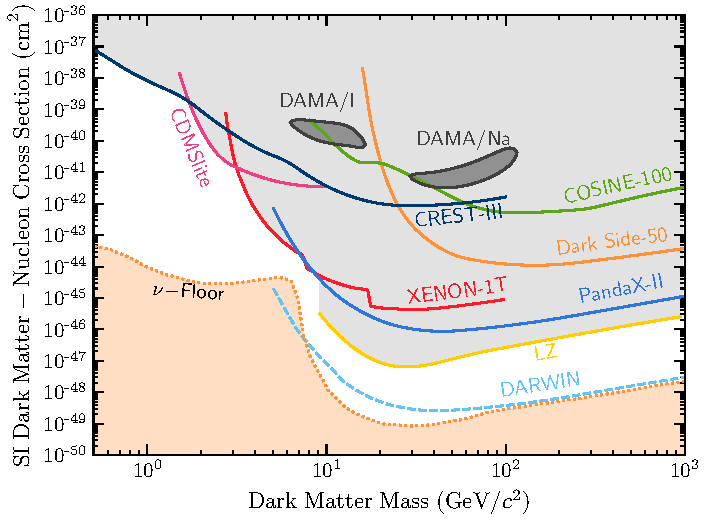
\includegraphics{DM_limits_SI.pdf}
    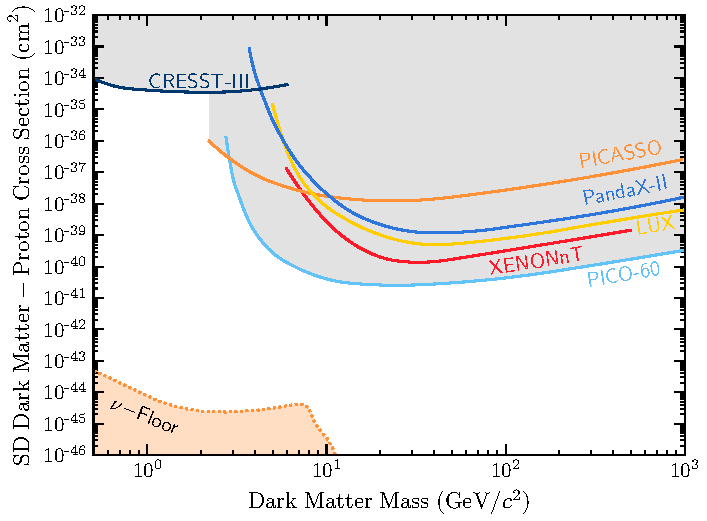
\includegraphics{DM_limits_SD_p.pdf}
    \caption{Current status of direct detection searches for dark matter. \textbf{Top:} Spin-independent dark matter-nucleon scattering. \textbf{Bottom:} Spin-dependent dark matter-proton scattering. Shaded regions above the coloured lines are excluded. Data was taken from the sources cited in the text.}
    \label{ch1:fig:direct_detection_lims}
\end{figure}

The current leading constraints on the dark matter-nucleon scattering cross-section
are shown in Fig.~\ref{ch1:fig:direct_detection_lims}, with SI in the top panel and SD in the bottom.
The SI limits are set by liquid noble gas experiments (LZ~\cite{LZ:2022lsv_jul_FirstDarkMatter}, 
XENON-1T~\cite{XENON:2020gfr_mar_SearchCoherentElastic}, PandaX-II~\cite{PandaX-4T:2021bab_dec_DarkMatterSearch},
and DarkSide-50~\cite{DarkSide:2022dhx_mar_SearchDarkMatterNucleon}), solid-state cryogenic detectors (CRESST-III~\cite{CRESST:2019jnq_nov_FirstresultsCRESSTIII}, CDMSlite~\cite{SuperCDMS:2023sql_jun_SearchLowmassDark}, with projected DARWIN sensitivities~\cite{Aalbers:2022dzr_dec_Nextgenerationliquidxenon}), 
and room temperature crystals (DAMA/LIBRA~\cite{Savage:2008er_CompatibilityDAMALIBRA}, and COSINE-100~\cite{COSINE-100:2021xqn_nov_StrongconstraintsCOSINE100}). 

The constraints on the SD dark matter-proton scattering cross-section are shown in the bottom panel of Fig~\ref{ch1:fig:direct_detection_lims}. 
Superheated liquid experiments such as the PICO-60~\cite{PICO:2019vsc_jul_Darkmattersearch} as well as PICASSO~\cite*{Behnke:2016lsk_apr_FinalResultsPICASSO} provide the leading constraints. 
These interactions are also constrained by many of the same experiments taht focus on SI interactions, as they will inevitably contain isotopes with non-zero spin, such as $\ce{^{129} Xe}$ and $\ce{^{131} Xe}$ in XENONnT. 

The orange dashed line represents the neutrino floor\footnote{Calling this the ``neutrino fog" rather than floor has been gaining traction in recent years~\cite{OHare:2021utq_dec_Foghorizonnew}}, providing a lower limit on the cross-section that can be probed by conventional direct detection experiments. Below this line, detectors will become sensitive to the irreducible background from Coherent Elastic Neutrino-Nucleus Scattering (CE$\nu$NS). For dark matter masses $\lesssim 10\GeV$ the solar neutrino flux is the main background source, while the atmospheric neutrino flux becomes the dominant background for masses $\gtrsim 20\GeV$. 
A significant amount of effort is being put toward overcoming this limitation, with the main strategy being to take advantage of the directionality of dark matter flux~\cite{Grothaus:2014hja_jun_DirectionalDarkMatter}. Such experiments attempt to resolve the direction of the nuclear recoil event, giving information about the direction the incident particle came from. This could allow discrimination between dark matter events, that are expected to be from the direction of the Cygnus constellation, and the background solar and atmospheric neutrinos coming from the Sun and sky respectively. 

Many experiments begin to lose sensitivity to low-mass dark matter ($m_\mathrm{DM}\lesssim 10\GeV$) as the recoil energy of the targets falls below the threshold energy resolution of the detector. Current detectors can reach thresholds as low as $\sim {\cal O} (100\eV)$, which is on the same order of magnitude as the recoil energy due to a $1\GeV$ dark matter collision. 

On the other hand, above $\sim 10\GeV$ the sensitivities of the experiments all decrease at a rate inversely proportional to the dark matter mass.  This is due to the interaction rate in Eq.~\ref{ch1:eq:DD_rate} being proportional to the number of dark matter particles that pass through the detector, $\NDM = \rho_\mathrm{DM}/m_\mathrm{DM}$. As the local dark matter density is observed to be $\rho_\mathrm{DM} = 0.4\GeV \cm^{-3}$, $\NDM$ decreases as the dark matter mass increases, and hence so do the detector sensitivities. 

Direct detection limits also assume that the scattering cross-section is independent of the dark matter velocity and momentum transfer in the interaction. Given that the local dark matter dispersion velocity is predicted to be $v_d = 270\km\s^{-1} \approx 10^{-3}c$, a back-of-the-envelope estimation for the momentum transfer gives $q_\mathrm{tr}\lesssim 100 \MeV$. Therefore, cross-sections proportional to $v_\mathrm{DM}$ or $q_\mathrm{tr}$ will result in significantly lower event rates and hence much weaker limits than the unsuppressed interactions. 

%%%%%%%%%%%%%%%%%%%%%%%%%%%%%%%%%%%%%
%%%%%%%%%%%%%%%%%%%%%%%%%%%%%%%%%%%%%
\subsection{Indirect Detection}
%%%%%%%%%%%%%%%%%%%%%%%%%%%%%%%%%%%%%
%%%%%%%%%%%%%%%%%%%%%%%%%%%%%%%%%%%%%

This leads us to indirect detection methods, which can provide complementary probes to direct detection while also exploring interactions that are difficult, if not impossible, for terrestrial-based detectors to observe.
Indirect detection experiments aim to infer the presence of dark matter through its annihilation or decay into Standard Model states. 
These searches look for dark matter annihilation products from astrophysical sources, including:
\begin{itemize}
    \item Gamma-rays at terrestrial-based telescopes such as HESS~\cite{HESS:2018cbt_may_SearchgRayLine, Montanari:2023bzn_jul_Searchdarkmatter, HESS:2006zwn_ObservationsGalacticCenter}, VERITAS~\cite{VERITAS:2017tif_apr_DarkMatterConstraints, Ryan:2023yzu_jul_SearchDarkMatter, McGrath:2023oto_jul_IndirectsearchDark, Ryan:2023yzu_jul_SearchDarkMatter}, MAGIC~\cite{MAGIC:2009tyk_MAGICGammaRayTelescope, MAGIC:2011nta_SearchesDarkMatter, MAGIC:2011nta_SearchesDarkMatter, MAGIC:2009tyk_MAGICGammaRayTelescope} and HAWC~\cite{HAWC:2017mfa_feb_DarkMatterLimits, HAWC:2017udy_feb_SearchDarkMatter, HAWC:2017udy_feb_SearchDarkMatter, HAWC:2017mfa_feb_DarkMatterLimits, Proper:2015xya_jul_FirstLimitsDark, Harding:2015bua_jul_DarkMatterAnnihilation} as well as the Fermi-LAT~\cite{Fermi-LAT:2015att_nov_SearchingDarkMatter,Fermi-LAT:2015kyq_jun_UpdatedSearchSpectral,Fermi-LAT:2012ugx_FermiLATSearch, Fermi-LAT:2010qeq_ConstraintsCosmologicalDark, Su:2010qj_GiantGammarayBubbles} satellite;

    \item Neutrino signals at IceCube~\cite{IceCube:2016dgk_mar_Searchannihilatingdark, IceCube:2012ugg_mar_Searchdarkmatter}, ANTARES~\cite{ANTARES:2016bxz_jun_SearchDarkMatter,ANTARES:2016obx_may_SearchSecludedDark,ANTARES:2016xuh_aug_LimitsDarkMatter}, Super-K~\cite{Super-Kamiokande:2015xms_apr_Searchneutrinosannihilation,Super-Kamiokande:2004pou_Searchdarkmatter,Feng:2008qn_TestingDarkMatter}, and will be searched for at the upcoming Hyper-K~\cite{Bell:2020rkw_sep_SearchingSubGeVDark,Bell:2021esh_nov_Searchingdarkmatter,Bell:2022ycf_nov_Darkmatterpollution}, JUNO~\cite{Franarin:2018gfk_jun_JUNOSensitivityResonant} experiments.

    \item Cosmic-Ray antimatter excess observed by the AMS-02 experiment~\cite{Giesen:2015ufa_sep_AMS02antiprotonslast, Bergstrom:2013jra_oct_NewLimitsDark}
\end{itemize}

Signals from dark matter annihilation are best searched for by looking at regions where the dark matter density is expected to be high, boosting the annihilation rate. 
Natural places to look include the Galactic Centre~\cite{Ipek:2014gua_sep_RenormalizableModelGalactic, Fermi-LAT:2017opo_may_FermiGalacticCenter}, dwarf-spheroidal galaxies~\cite{Bonnivard:2015xpq_oct_Darkmatterannihilation}, and celestial bodies where dark matter can accumulate over time. The latter scenario is central to this work and was pioneered by considering the effects of dark matter being captured within the Sun.



%%%%%%%%%%%%%%%%%%%%%%%%%%%%%%%%%%%%%
%%%%%%%%%%%%%%%%%%%%%%%%%%%%%%%%%%%%%
\section{Dark Matter Signals from the Sun}
%%%%%%%%%%%%%%%%%%%%%%%%%%%%%%%%%%%%%
%%%%%%%%%%%%%%%%%%%%%%%%%%%%%%%%%%%%%

Stars have a rich history of being used as astrophysical laboratories to help in the search for dark matter. Depending on the type of dark matter being searched for, there are various signals one can look for.
Light bosonic dark matter, such as ALPs and dark photons, can be produced within the plasma of stars, altering the energy transport properties within them.
This can ultimately lead to deviations in the evolution of the star, which can be used to place some of the strongest constraints on these models~\cite{An:2013yfc_oct_Newstellarconstraints, Dolan:2022kul_oct_Advancingglobularcluster, Dolan:2023cjs_jun_ConstrainingDarkPhotons}.
WIMP-like dark matter in the halo that couples to visible matter can scatter within the stars as they pass through. 
If the dark matter loses enough energy in these interactions, it can become gravitationally bound to the object and a population of dark matter will be accumulated within the star over time~\cite{Press:1985ug_Capturesungalactic, Gould:1987ju_WeaklyInteractingMassive, Gould:1987ir_ResonantEnhancementsWIMP, Jungman:1995df_Supersymmetricdarkmatter, Busoni:2017mhe_oct_Evaporationscatteringmomentum}. 

This idea of WIMPs accumulating within the cores of stars has been applied extensively to the star closest to us, the Sun. The formalism for stellar capture of dark matter was set up by Gould~\cite{Gould:1987ir_ResonantEnhancementsWIMP, Gould:1987ju_WeaklyInteractingMassive,Gould:1991va_Bigbangarcheology} in the late 80's, and has remained quite successful to this day,  with many authors continuing to build upon these foundations over time~\cite{Busoni:2017mhe_oct_Evaporationscatteringmomentum,Garani:2017jcj_may_DarkmatterSun,Bramante:2017xlb_sep_Multiscatterstellarcapture}.

Once the dark matter is captured, it will continue to scatter with the stellar constituents until it thermalises within the core of the Sun, collecting with an isothermal sphere. The radius of this sphere can be found by applying the virial theorem, with the gravitational potential given by
\begin{align}
    \Phi(r) & = -\int_r^\infty \,\frac{G M_\odot(r')}{r'^2}dt',\\
    &\approx \frac{2}{3}\pi G \rho_{\odot,c} r^2,
\end{align}
assuming the density of the Sun within this region is constant, $\rho_{\odot,c}$. The resulting radius is
\begin{equation}
    r_\mathrm{iso}^2 = \frac{3 T_\odot}{2\pi G \mdm \rho_\odot}.
\end{equation}
The dark matter number density will follow a Gaussian profile, 
\begin{align}
    n_\mathrm{iso}(r) &= n_0\exp\left( - \frac{\mdm \Phi(r)}{T_\odot}\right),\\
     & = n_0 \exp(-r^2/r_\mathrm{iso}^2),
\end{align}
where $n_0$ is a normalistion constant fixed by requiring that the total number of dark matter particles is 
\begin{equation}
    \NDM = \int d^3 r\, \niso(r).
\end{equation}
In addition, dark matter velocity will follow a Maxwell-Boltzmann distribution, 
\begin{equation}
    \fMB(v) = 4\pi\left(\frac{\mdm}{4\pi T_\odot}\right)^{3/2}v^2\exp\left[-\frac{\mdm v^2}{4 T_\odot}\right].
\end{equation}

The time evolution of the total number of dark matter particles within the Sun is governed by three processes. Capture acts to increase the number over time, while annihilation and evaporation will reduce this number over time. This is described by the differential equation
\begin{equation}
    \frac{d \NDM}{dt} = C  - E \NDM- A \NDM^2,
    \label{ch1:eq:DM_num_Sun}
\end{equation}
where $C$ and $E$ are the capture and evaporation rates respectively, with $A$ being related to the annihilation rate, $\GAnn$ through
\begin{align}
    \GAnn & = \frac{1}{2}\int\,dr^3 n_\mathrm{iso}^2(r) \sigmavdm\\
    & \equiv \frac{1}{2}A \NDM^2,
\end{align}
where the factor of 1/2 accounts for each annihilation removing two dark matter particles from the Sun. 

In this context, evaporation refers to the process in which dark matter can be ejected back out of the Sun by up-scattering\footnote{Up-scattering refers to the interactions in which the dark matter gains rather than loses energy. } off an energetic constituent. This becomes increasingly important for lighter dark matter masses, as less energy will be required to boost the dark matter above the local escape velocity. Below a certain mass, the capture and evaporation come into equilibrium, and a net-zero amount of dark matter is contained within the Sun.
This critical mass places a lower bound on the dark matter mass that can be probed through stellar capture and is named the evaporation mass, $\mevap$. 

There are three regimes we are interested in solving this equation for. The simplest case is when evaporation and annihilation are both negligible, then the solution is simply, 
\begin{equation}
    \NDM(t) = C t,
\end{equation}
indicating that the dark matter will simply continue to grow over time.

Next,  assume that annihilations are negligible ($A = 0$), while capture and evaporation are present. The result is
\begin{equation}
    \NDM(t) = Ct\left(\frac{1 - e^{-E t}}{E t}\right),  
\end{equation}
where the first factor is the number of captured dark matter if evaporation is negligible. From this, we can estimate the evaporation mass by asking when the evaporation rate is large enough to cause a significant reduction in the number of captured dark matter particles relative to the $E=0$ case. This can be expressed formally as~\cite{Garani:2017jcj_may_DarkmatterSun}
\begin{equation}
    \frac{1}{\NDM(\mevap)}\left| \NDM(\mevap) - \frac{C(\mevap)}{E(\mevap)} \right| = \alpha,
\end{equation} 
where $\alpha$ is the fraction of evaporated dark matter, taken to be $\sim 10\%$. 

Finally, consider the case in which evaporation can be neglected, $\mdm\gtrsim \mevap$. The solution in this regime is
\begin{equation}
    \NDM(t) = \sqrt{\frac{C}{A}}\tanh(\sqrt{CA}t)\overset{t\rightarrow\infty}{\longrightarrow} \sqrt{\frac{C}{A}},
\end{equation}
that reaches an equilibrium state between capture and annihilation for times longer than the characteristic scale, $\teq = 1/\sqrt{CA}$. This state is known as capture-annihilation equilibrium.

The signals searched for depend on whether the dark matter can annihilate or not. If the dark matter is asymmetric, it cannot annihilate, and we can set $A = 0$ in Eq.~\ref{ch1:eq:DM_num_Sun}. This leads to the population continuing to grow over time, with $\NDM(t) = Ct$ if evporation is negligible. A large enough population of captured dark matter can alter the energy transport within the Sun, leading to the modifications of the solar neutrino flux, or even the solar structure itself~\cite{Franarin:2018gfk_jun_JUNOSensitivityResonant, Cumberbatch:2010hh_LightWIMPsSun, Vincent:2013lua_apr_Thermalconductiondark,Vincent:2015gqa_aug_Generalisedformfactor}. 

Instead, if the dark matter can annihilate an equilibrium will eventually be reached between the capture and annihilation rates, and the total number of dark matter particles will be constant. If the annihilation products can escape the Sun, they can be searched for by various experiments depending on the nature of the final states.
These could be neutrinos produced from the decays of other charged annihilation products~\cite{Super-Kamiokande:2011wjy_IndirectSearchWIMPs,Super-Kamiokande:2015xms_apr_Searchneutrinosannihilation,ANTARES:2016obx_may_SearchSecludedDark,ANTARES:2016xuh_aug_LimitsDarkMatter,IceCube:2016dgk_Searchannihilatingdark}, or to some other long-lived state that can escape the Sun and decay into visible states~\cite{Batell:2009zp_SolarGammaRays,Schuster:2009au_TerrestrialSolarLimits,Bell:2011sn_Enhancedneutrinosignals,Feng:2016ijc_jun_DarkSunshineDetecting,Leane:2017vag_jun_PowerfulSolarSignatures}.


\begin{figure}[!t]
    \centering
    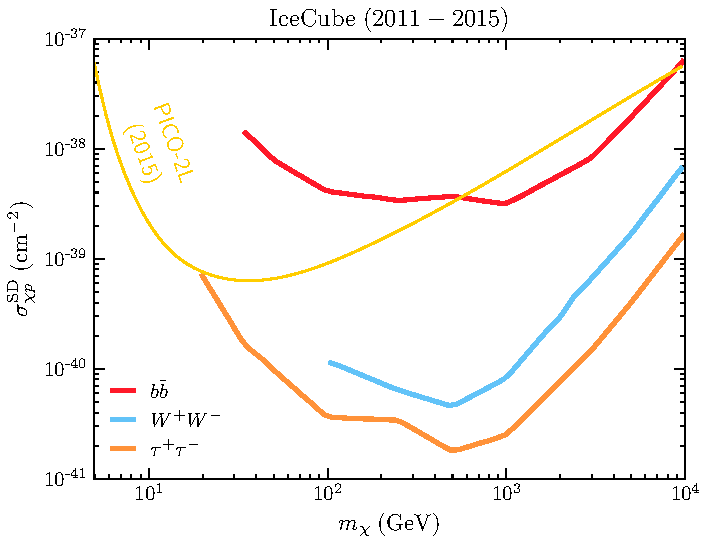
\includegraphics{IceCube_2016.pdf}
    \caption{Limits on the SD dark matter-proton cross-section from the IceCube collaboration assuming 100\% branching fraction to $b\bar{b}$ (red), $W^+ W^-$ (blue) or $\tau^+ \tau^-$ (orange) final states. Also shown is the result from the PICO-2L DD experiment. This plot was recreated with data taken from Ref.~\cite{IceCube:2016dgk_mar_Searchannihilatingdark}.}
    \label{ch1:fig:IceCube_2016_SD}
\end{figure}

In comparison to DD searches, interpretation of indirect detection data will require additional model-dependent assumptions, namely the relevant annihilation channels of the dark matter. 
The most general limits can be placed by assuming that the dark matter only has a single annihilation channel, i.e. annihilation to a $\tau^+\tau^-$ final state 100\% of the time. 
Under these assumptions, limits on the SD dark matter-proton cross-section have been placed that exceed current DD constraints, due to the rather large abundance of Hydrogen within the Sun. Constraints from the IceCube collaboration are shown in Fig.~\ref{ch1:fig:IceCube_2016_SD}.

As stated above, the range of dark matter masses that can be probed by Solar capture is limited by the evaporation mass of $\sim 3\GeV$. Additionally, as with direct detection, interactions that are suppressed by the momentum transfer/velocity of the dark matter will result in a significantly smaller capture rate and hence a smaller flux of annihilation products, resulting in weaker limits. These constraints also rely on the annihilation rate being sufficiently fast such that capture-annihilation equilibrium is reached within the lifetime of the Sun. If the annihilation cross-section is $p$-wave suppressed by the velocity of the annihilating dark matter, then this equilibrium may not be achieved. Should this be the case, then no limits can be placed as no flux of annihilation products to detect. 

Overcoming the first of these issues requires either a colder star or one that is much heavier to decrease the evaporation mass. The second requires dark matter to scatter with the constituent material at relativistic energies to overcome the suppression in the cross-sections. Finally, the $p$-wave suppression can be alleviated if the dark matter annihilates within a very small volume in the core of the star, boosting the annihilation rate.
Fortunately, there exist objects that can achieve all of these requirements, allowing for a wider variety of dark matter models to be explored than direct detection or traditional indirect detection experiments. These objects are known as compact objects, namely neutron stars and white dwarfs.

%%%%%%%%%%%%%%%%%%%%%%%%%%%%%%%%%%%%%
%%%%%%%%%%%%%%%%%%%%%%%%%%%%%%%%%%%%%
%%%%%%%%%%%%%%%%%%%%%%%%%%%%%%%%%%%%%
\section{Compact Objects as Dark Matter Probes}
%%%%%%%%%%%%%%%%%%%%%%%%%%%%%%%%%%%%%
%%%%%%%%%%%%%%%%%%%%%%%%%%%%%%%%%%%%%
%%%%%%%%%%%%%%%%%%%%%%%%%%%%%%%%%%%%%

The main goal behind this work is to explore how compact objects can be used to probe a wide variety of dark matter interactions that terrestrial direct detection experiments are insensitive to. By compact objects, we are referring to Neutron Stars (NSs) and White Dwarfs (WDs), and not Black Holes that also fall into this category.


Compact objects offer a unique laboratory for studying dark matter and its interactions with the Standard Model in environments unachievable anywhere else in the Universe. They generate strong gravitational fields and are composed of incredibly dense matter, with NSs reaching super-nuclear densities in their central cores. The capture rate within these objects is therefore enhanced due to these properties, with benefits over solar capture including:


\begin{itemize}
\item \textbf{Gravitational focusing of the DM flux:} The strong gravitational field will increase the impact parameter of the infalling dark matter. This increases the effective size of the capturing body, increasing the flux of dark matter passing through it. 

\item \textbf{Realtivistic Interaction Energies:} In general, the infalling dark matter will be accelerated to (semi-)relativistic velocities ($\sim 0.2 - 0.7 c$). Moreover, the stellar constituents will also have relativistic energies. As such, interactions that are momentum/velocity dependent will suffer far less suppression than in DD experiments. 

\item \textbf{Large Number of Targets:} The extremely high densities of these objects correspond to a considerable number of targets for scattering to occur. This allows these objects to probe very small scattering cross-sections, with NSs in particular expected to reach as low as $\sim 10^ {-45}\cm^2$. 

\item \textbf{Low Evpaortion Masses}: Relative to the Sun, the evaporation mass in compact objects can be quite low, on the order of keV in some cases. This is due in part to the increased gravitational strength, but mainly to the significantly lower temperatures in old compact objects. 
\end{itemize}

In the past, capture in NSs has been applied primarily in the context of seeding gravitational collapse into black holes~\cite{McDermott:2011jp_ConstraintsScalarAsymmetric,Kouvaris:2011fi_ExcludingLightAsymmetric,Guver:2012ba_may_Capturedarkmatter, Garani:2018kkd_may_NewAnalysisNeutron,Bramante:2013nma_jan_Boundsselfinteractingfermion,Bertoni:2013bsa_dec_DarkMatterThermalization,Bell:2013xk_jun_Realisticneutronstar}, and the modifications of NS merger rates as well as the gravitational wave signatures of these mergers~\cite{Bramante:2017ulk_mar_SearchingDarkMatter, Ellis:2017jgp_jun_SearchDarkMatter, Ellis:2018bkr_jun_DarkMatterEffects,Nelson:2018xtr_jul_Darkhalosneutron}. Capture in WDs has also been considered, with a variety of different applications of the capture process~\cite{Steigerwald:2019efv_dec_DarkMatterThermonuclear, Panotopoulos:2020kuo_jun_Constraintslightdark, McCullough:2010ai_CaptureInelasticDark, Hooper:2010es_InelasticDarkMatter, Bramante:2015cua_sep_Darkmatterignition, Bertone:2007ae_CompactStarsDark}. 

In recent years, dark matter induced heating of NSs has reemerged as a potential detection frontier~\cite{Raj:2017wrv_feb_Neutronstarsdark, Baryakhtar:2017dbj_sep_DarkKineticHeating, Bell:2018pkk_sep_HeatingNeutronStars,Joglekar:2019vzy_sep_Relativisticcapturedark, Acevedo:2019agu_mar_WarmingNuclearPasta, Bell:2019pyc_jun_CaptureLeptophilicDark, Garani:2019fpa_aug_Darkmatterinteractions,Chatterjee:2022dhp_jul_Faintlightold}. It was shown that dark matter could reheat old, isolated NSs in our local neighbourhood\footnote{Local neighbourhood refers to the region within $\sim 1\kpc$ of the Sun.} back up to temperatures that would cause them to radiate as blackbody peaked in the near-infrared. 
The aim is to locate the NSs with radio telescopes such as the Square-Kilometer-Array (SKA), and determine their age through their spin-down rate. 
Once located, the star's temperature can be determined through observations from infrared telescopes such as the James Webb Space Telescope (JWST). Knowing the age of the star allows us to compare its observed temperature to that predicted by models of neutron star cooling. A discrepancy between these two temperatures can indicate whether an additional heating source is present within the star. 

This heating occurs in two stages. The dark matter will first kinetically heat the star through the scattering events that result in both its capture and thermalisation. We define \textit{kinetic hearing} to have been achieved once the dark matter has deposited $99\%$ of its initial kinetic energy into the star.
If the dark matter can annihilate, and assuming these annihilation products remain trapped within the star, its mass energy will be transferred to the star, further increasing the temperature of the star. In order for this \textit{annihilation heating} to be efficient, capture-annihilation equilibrium must be achieved on a timescale shorter than the age of the star. These processes are illustrated in Fig.~\ref{ch1:fig:cartoon_NS_heat}, with the temperatures shown assuming a NS in our local neighbourhood.


\begin{figure}[!t]
    \centering
    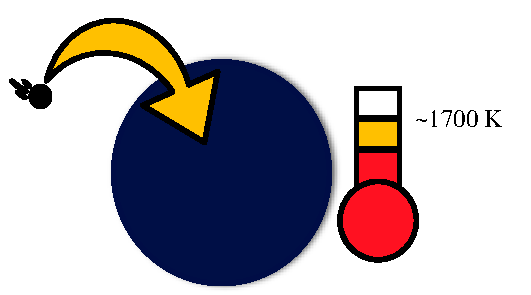
\includegraphics[width=0.45\textwidth]{kin_heat_NS.pdf}
    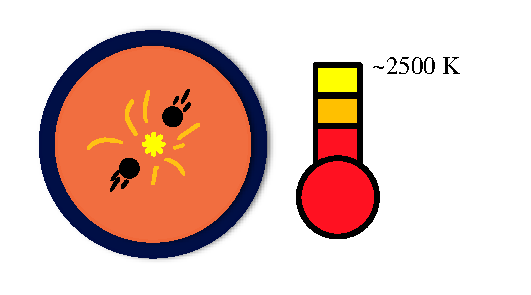
\includegraphics[width=0.45\textwidth]{ann_heat_NS.pdf}
    \caption{Illustration of DM-induced heating of compact objects. \textbf{Left:} kinetic heating due to DM scattering, raising the temperature to $\sim 1700 \K$. \textbf{Right:} Annihilation heating contributes an additional $\sim 800\K$. This image is inspired by Ref.~\cite{Raj:2017wrv_feb_Neutronstarsdark}.}
    \label{ch1:fig:cartoon_NS_heat}
\end{figure}

It is important to keep track of all the timescales involved in the heating process so that we can accurately determine the full extent of dark matter-induced heating. These timescales are the age of the star, $\tstar$, the kinetic heating time, $\tkin$, and the capture-annihilation heating timescale, $\teq$. In order for maximal heating to be achieved, we require $\tkin + \teq < \tstar$. 

To accurately project how sensitive neutron star heating to dark matter interactions, one first requires an accurate calculation of the capture rate. However, existing calculations have relied on the formalism set up by Gould for capture in the Sun without fully accounting for the extreme physics present in these objects. Developing a consistent formalism for dark matter capture in compact objects, based on the Gould formalism, and applying this to dark matter induced heating is at the heart of this thesis.  

%%%%%%%%%%%%%%%%%%%%%%%%%%%%%
%%%%%%%%%%%%%%%%%%%%%%%%%%%%%
\section{Thesis Outline}
%%%%%%%%%%%%%%%%%%%%%%%%%%%%%
%%%%%%%%%%%%%%%%%%%%%%%%%%%%%

Following this introduction, Chapter~\ref{chapter:compactobjects} covers the prerequisite knowledge of compact objects
required for the remainder of this work. This includes a detailed overview of the general structure equations of relativistic stars, followed by details of the internal structure of both white dwarfs and neutron stars. 

Chapters~\ref{chapter:capture_1} and~\ref{chapter:capture_2} of this thesis are devoted to reformulating Gould's capture formalism to account for the physics specific to compact objects in a self-consistent manner. These include a relativistic treatment of the kinematics, using General Relativity to calculate the correct dark matter flux passing through the star, and accounting for Pauli blocking of the final state target using Fermi-Dirac statistics for the stellar constituents. In addition, we incorporate the internal structure of these objects by calculating the radial profiles for the relevant microscopic quantities (e.g., chemical potentials and number densities) via the adoption of a realistic equation of state.

Further considerations are required when considering dark matter interactions with the baryonic matter inside NSs. Due to the high density of the NS interior, the baryons undergo strong self-interactions and should not be treated as a free Fermi gas. Instead, adopting an equation of state that accounts for these interactions is required. These interactions modify the mass of the baryons, leading them to obtain an effective mass smaller than their value in vacuum. Furthermore, as we will see, the dark matter may interact with the baryons with momentum transfers on the order of $10\GeV$. This is high enough that the dark matter will begin to resolve the internal structure of the baryon. To account for this, the momentum dependence of the baryon form factors that are typically neglected in direct detection and solar capture must be reintroduced.

This formalism is made in preparation for a thorough analysis of the timescales involved in the dark matter heating of compact objects, covered in Chapter~\ref{chapter:thermalisation}. The energy deposited in both the kinetic and annihilation heating stages does not occur instantaneously, and the timescales involved in them need to be compared to the age of the star in question. We will define kinetic heating timescale as the time required for dark matter to deposit 99\% of its initial kinetic energy into the star. For annihilation heating to occur, the dark matter must reach a state of capture-annihilation equilibrium within the stellar core. In standard calculations of this timescale, the dark matter must first become thermalised with the star. Only then can annihilations occur efficiently enough to heat the star. 


We will work with the EFT operators in Table~\ref{ch1:tab:opers_defn_full} that describe Dirac fermion dark matter interacting with Standard Model fermions. Each operator will be studied in isolation, i.e., by considering a Lagrangian that contains only one of the operators rather than a linear superposition of multiple. This way, we can analyse specific types of interactions independently, allowing us to take as model-independent an approach to the phenomenology as possible. 

We present our concluding remarks on this thesis in Chapter~\ref{chapter:conclusion}.
  
  %% Compact Objects 
  \graphicspath{{img/compact_objects/}}



\chapter{A Primer on Compact Objects}
\label{chapter:compactobjects}

% \begin{synopsis}
% Introduce COs, formation, structure etc...  
% \end{synopsis}
%%%%%%%%%%%%%%%%%%%%%%%%%%%%%%%%%%%%%
%%%%%%%%%%%%%%%%%%%%%%%%%%%%%%%%%%%%%
%%%%%%%%%%%%%%%%%%%%%%%%%%%%%%%%%%%%%

Within the cores of stars, there exists a delicate balance between the gravitational forces pulling the matter inward and the outward pressure generated by the thermonuclear fusion of light elements. This process begins as hydrogen is fused to form helium. Eventually, the hydrogen is depleted, allowing gravity to temporarily overcome the outward pressure, leading to the core to begin contracting. As this occurs, the gravitational potential energy is converted to thermal energy, and the core eventually becomes hot enough to facilitate helium burning. 

This cycle can continue as heavier and heavier elements are formed within the ever-increasingly hot stellar core. Lighter stars cannot reach the temperatures required to fuse light elements such as helium and carbon. If the star is heavy enough, iron will eventually be formed from the burning of silicon. As the fusion of iron nuclei is an endothermic process, it will not occur spontaneously, ending the cycle in heavy stars. Without a fuel source, the core will collapse under its gravity, leading to the death of the star.

What comes after this collapse depends on the mass of the progenitor star. Very light stars, $\lesssim 0.5 \Msun$, have lifetimes much longer than the age of the universe and so are uninteresting to our current discussion. Moderately heavy stars, $1\Msun\lesssim \Mstar \lesssim 8\Msun$, will continue burning fuel until the outer layers of the star are dispersed as it expands, leaving a core comprised of helium, carbon, and oxygen with and small abundance of heavier elements. In this case, the core will begin to collapse until the Fermi degeneracy of the ultrarelativistic electrons is great enough to reestablish equilibrium, resulting in a White Dwarf (WD)~\cite{Jackson:2004vt_Compactobjectseveryone}.

Heavy stars, $\gtrsim 8\Msun$, spectacularly end their lives in a type-II supernova event. This occurs when the core of the star exceeds the Chandrashekhar mass of $1.4\Msun$, which cannot be supported by electron degeneracy pressure. The core itself will then collapse, leading to a shockwave that ejects the majority of the mass of the star. All that will remain is an extremely dense core supported by neutron degeneracy pressure: a Neutron Star (NS)~\cite{Woosley:2005cha_PhysicsCoreCollapseSupernovae}. If the star was so massive that the gravitational forces overcome even the neutron degeneracy pressure, then the core collapses into a black hole. 

These stellar corpses, white dwarfs, neutron stars, and black holes are collectively known as compact objects. They have masses similar to or larger than the Sun, compressed into much smaller bodies resulting in a significantly larger surface gravity. These objects do not have a source of fuel and, as such, spend the rest of their lives cooling through the emission of photons and neutrinos. For the remainder of this thesis, we will only be interested in white dwarfs and neutron stars and will collectively refer to these as compact objects, excluding black holes from this term. 

This chapter is dedicated to discussing the aspects of the structure, composition, and observational status of compact objects relevant to this work
% \footnote{As this work is written from the perspective of a particle physicist, I wish to apologise to my astrophysics colleagues for what is to come.}. 

%%%%%%%%%%%%%%%%%%%%%%%%%%%%%%%%%%%%%
%%%%%%%%%%%%%%%%%%%%%%%%%%%%%%%%%%%%%
%%%%%%%%%%%%%%%%%%%%%%%%%%%%%%%%%%%%%
\section{Structure Equations from General Relativity}
\label{ch2:sec:CO_general_structure}
%%%%%%%%%%%%%%%%%%%%%%%%%%%%%%%%%%%%%
%%%%%%%%%%%%%%%%%%%%%%%%%%%%%%%%%%%%%

Being comprised of matter in a highly dense state, the gravitational fields produced by neutron stars and white dwarfs are extremely strong.
As such, modelling the structure of these objects falls into the domain of General Relativity (GR). Here we review the structure of static, spherically symmetric, compact objects, adapting the discussions in Refs.~\cite{Shapiro_Blackholeswhite, Misner_Gravitation, Schutz_Firstcoursegeneral}. 

First, the static nature of the star means that the components of the metric are functions only of the spatial coordinates and not of time. Together with the assumption that the mass distribution of the star is spherically symmetric, this leads to a Schwarzschild-like metric of the form
\begin{equation}
    ds^2 = -d\tau^2 = -B(r) dt^2 + A(r) dr^2 + r^2 d\Omega^2,
    \label{ch2:eq:general_Swch_metric}
\end{equation}
with $d\tau$ the proper time interval. The functions $A(r),\; B(r)$ depend only on the radial coordinate, and are often written as 
\begin{equation}
    A(r) = e^{2\Lambda(r)},\quad B(r) = e^{2\Phi(r)}.
\end{equation}
These functions are subject to the condition that at distances far from the star, $r\rightarrow\infty$, space-time must become flat, which translates to the boundary conditions 
\begin{equation}
    \lim_{r\rightarrow \infty} A(r) = \lim_{r\rightarrow \infty} B(r)  = 1.
\end{equation}
% 
The matter within the star can be modelled as a perfect fluid, meaning we are neglecting any shear stresses and energy transport within the star. Such a fluid is described by its pressure $P(r)$, density $\rho(r)$, and baryonic number density, $n_b(r)$, as well as the 4-velocity of the fluid $u^\mu(r)$. Being static, the only non-zero component of this velocity is the $\mu = 0$ component,
% \footnote{Here we are using the convention of labeling the components of a 4-vector by the coordinates of the metric. For spherical coordinates, these are $\mu = (t, r, \theta, \phi)$ as opposed to the more general convention of having $\mu = (0, 1,2,3)$.}
which is fixed by the normalisation condition $g_{\mu\nu}u^\mu u^\nu = -1$ to be $u^0 = 1/\sqrt{B(r)}$.
These quantities are used to construct the stress-energy tensor of the star, which takes the form
\begin{equation}
    T^{\mu\nu} = (\rho + P)u^\mu u^\nu + P g^{\mu\nu}.
\end{equation}
The physics describing the underlying microscopic interactions within matter are encoded in an equation of state (EoS) that describes the relationship between the various thermodynamic quantities. This is typically expressed by providing the pressure as a function of the density, $P(\rho)$. It is often more convenient to parameterise the EoS by the number density of baryons $n_b$, and the entropy per baryon $s$, such that
\begin{equation}
    P=P(n_b, s), \quad \rho = \rho(n_b, s).
\end{equation}
The dependence on $s$ turns out to be trivial in most scenarios involving compact objects, such as those considered throughout this work. The pressure in these stars arises from the degeneracy of the nucleons in NSs or the electrons in WDs, rather than from the thermal motion of the constituents as in main sequence stars. These thermal degrees of freedom will be frozen out at temperatures lower than the Fermi energy of the system, which is typically around $E_F \sim 10\MeV$ in NSs or $\sim 1 \MeV$ in WDs, and correspond to temperatures of $T_\star\sim 10^{11}\K$ and $\sim 10^{10}\K$ respectively. As these objects are expected to cool well below these temperatures quickly after formation~\cite{Yakovlev:2004iq_Neutronstarcooling,Yakovlev:2004yr_Neutronstarcooling, Bedard_oct_Spectralevolutionhot}, the entropy can be taken to be zero throughout the star. This allows us to reduce the two-parameter EoS to a simpler one-parameter one,
\begin{equation}
    P=P(n_b, s = 0) = P(n_b), \quad \rho = \rho(n_b, s=0) = \rho(n_b).\label{ch2:eq:1_param_EoS}
\end{equation} 
% 
The structure of the star is therefore dictated by the quantities $A(r)$, $B(r)$, $P(r)$, $\rho(r)$, and $n_b(r)$. This system is determined by applying the Einstein field equations, $G^{\mu\nu} = 8\pi T^{\mu\nu}$, together with the energy-momentum conservation, $T^{\mu\nu}_{\quad;\nu}=0$, the EoS relations Eqs.~\ref{ch2:eq:1_param_EoS}, and the appropriate boundary conditions. The structure equations that come out of this analysis were first discovered concurrently by Tolman~\cite{Tolman:1939jz_StaticSolutionsEinstein} and by Oppenheimer and Volkoff~\cite{Oppenheimer:1939ne_MassiveNeutronCores}, and so are known as the TOV equations. They take the form
\begin{align}
    \frac{dP}{dr} &= -\rho(r) c^2  \left[ 1 + \frac{P(r)}{\rho(r) c^2} \right]\frac{d\Phi}{dr},\label{ch2:eq:TOV_1}\\
    \frac{d\Phi}{dr} & = \frac{G M(r)}{c^2 r^2} \left[ 1 + \frac{4\pi r^3 P(r)}{M(r)c^2} \right] \left[ 1 - \frac{2 G M(r)}{c^2 r}\right]^{-1}\label{ch2:eq:TOV_2},\\
    \frac{dB}{dr} & = 2B(r) \frac{d\Phi}{dr},\label{ch2:eq:TOV_3}
\end{align}
where $M(r)$ is related to the metric factor $A(r)$ through
\begin{equation}
    A(r) = \left[ 1 - \frac{G M(r)}{c^2 r} \right]^{-1},
\end{equation}
and is interpreted as the mass contained within a radius $r$. It obeys the mass equation 
\begin{equation}
    \frac{dM}{dr} = 4\pi r^2 \rho(r),\quad M(0) = 0,
    \label{ch2:eq:mass_equation_TOV}
\end{equation}
which arises from the $\mu = \nu = 0$ component of the Einstein field equations. 
These equations are the general relativistic versions of the hydrostatic equilibrium equations of regular stellar structure, with Eq.~\ref{ch2:eq:TOV_1} reducing to the familiar 
\begin{equation}
    \frac{dP}{dr} = -\frac{GM(r)}{r^2}\rho(r),
\end{equation}
in the Newtonian limit, $GM(r)/c^2 r \ll 1$.

The radius of the star, $\Rstar$, is identified as the point at which the pressure and density vanish, $P(\Rstar) = \rho(\Rstar) = 0$. In the region outside the star, $r>\Rstar$, the total mass remains constant at the total mass of the star, $M(r \geq  \Rstar) = \Mstar$, and so the only non-trivial structure functions in this region are the metric factors. Solving Eq.~\ref{ch2:eq:TOV_3} for $B(r)$ with $P(r)=0$ and constant $M(r) = M_\star$ leaves us with
\begin{equation}
    A(r) = \left[ 1 - \frac{G \Mstar}{c^2 r} \right]^{-1}, \quad B(r) = 1 - \frac{G \Mstar}{c^2 r} ,\quad\mathrm{for}\;r > \Rstar,
\end{equation}
and the metric reduces to the familiar Schwarzschild metric outside the star. 
Continuity of the metric at $r= \Rstar$ enforces a second boundary condition for $B(r)$,
\begin{equation}
    B(\Rstar) = 1 - \frac{G \Mstar}{c^2 \Rstar}.
    \label{ch2:eq:B_boundary_condition}
\end{equation}
% 
The final boundary condition required is the central pressure $P(0) = P_c$ or, equivalently, the central density/baryon number density. This is the only free parameter in the system and, hence, uniquely determines the stellar structure for a given EoS. Therefore, all the stars predicted by solving the coupled TOV + EoS system can be represented by a one-parameter sequence, represented by the mass-radius relation for the EoS model.


Given all the above, we can write a simple recipe for constructing a model of a compact object:
\begin{enumerate}
    \item Model the constituent matter with an appropriate EoS.
    \item Specify the central pressure of the star, $P_c$.
    \item Integrate the coupled system of differential equations \ref{ch2:eq:TOV_1}, \ref{ch2:eq:TOV_2}, \ref{ch2:eq:mass_equation_TOV} from the centre of the star outward until the pressure vanishes.
    \item Use the boundary condition Eq.~\ref{ch2:eq:B_boundary_condition} to normalise the metric function $B(r)$. 
\end{enumerate}
In general, additional quantities will be present in the EoS, such as chemical potentials and the speed of sound, which may be subject to additional constraints. These quantities will need to be calculated at each step of the integration alongside the other structure functions. 

%%%%%%%%%%%%%%%%%%%%%%%%%%%%%%%%%%%%%
%%%%%%%%%%%%%%%%%%%%%%%%%%%%%%%%%%%%%
%%%%%%%%%%%%%%%%%%%%%%%%%%%%%%%%%%%%%
\section{White Dwarfs}
\label{ch2:sec:white_dwarfs}
%%%%%%%%%%%%%%%%%%%%%%%%%%%%%%%%%%%%%
%%%%%%%%%%%%%%%%%%%%%%%%%%%%%%%%%%%%%
%%%%%%%%%%%%%%%%%%%%%%%%%%%%%%%%%%%%%

The fate of main sequence stars of mass below $\Mstar \lesssim 8 \Msun$ is to end their lives as a white dwarf. Consequently, these compact stellar remnants, which are supported against gravitational collapse by electron degeneracy pressure, are the most abundant stars in the Galaxy ($\gtrsim 90\%$). They are born at very high temperatures and cool down over billions of years. Observations of the coldest WDs, therefore, contain information about the star formation history of the Galaxy.

The vast majority of observed WDs are composed primarily of carbon and oxygen, plus small traces of elements heavier than helium. 
At the extremely high densities found in WDs, $\rho_\star\sim 10^6-10^{10}\g\cm^{-3}$, electrons are strongly degenerate and determine the WD equation of state (EoS) and internal structure.  The stellar core resembles a Coulomb lattice of ions surrounded by the degenerate electron gas, implying that the WD core is isothermal and a very good thermal conductor. 
The degenerate core is enclosed by a thin envelope that accounts for $\lesssim 1\%$  of the total mass~\cite{Fontaine_apr_Potentialwhitedwarf}. 

The outer layers form an atmosphere rich in lighter elements such as hydrogen or helium. The exact composition depends on the evolution of the WD progenitor and changes as the WD cools. 
This atmosphere is non-degenerate and extremely opaque to radiation, with an EoS that is subject to finite temperature effects. We limit our discussion to the core region of the WD, which accounts for the vast majority of its mass.

%%%%%%%%%%%%%%%%%%%%%%%%%%%%%%%%%%%%%
%%%%%%%%%%%%%%%%%%%%%%%%%%%%%%%%%%%%%
\subsection{The FMT Equation of State}
\label{ch2:sec:FMT_EoS}
%%%%%%%%%%%%%%%%%%%%%%%%%%%%%%%%%%%%%
%%%%%%%%%%%%%%%%%%%%%%%%%%%%%%%%%%%%%


In the limit of zero temperature, the simplest way to obtain the WD EoS is to assume an ideal Fermi gas of degenerate electrons within a WD that is composed of a single element. Corrections to the non-interacting electron picture were introduced early by Salpeter~\cite{Salpeter:1961zz_nov_Energypressurezerotemperature}. By introducing the Wigner-Seitz (WS) cell approximation and assuming point-like nuclei, Salpeter obtained an analytical EoS that accounts for interactions between electrons and ions as well as other Coulomb corrections. These corrections, in general, depend on the chemical composition of the star. 

More recently, it has been shown that the treatment of matter at high pressures presented by Feynman, Metropolis and Teller~\cite{Feynman:1949zz_Equationsstateelements} can be extended to consistently take into account weak interactions and relativistic effects \cite{Rotondo:2009cr_RelativisticThomasFermitreatment, Rotondo:2011zz_RelativisticFeynmanMetropolisTellertheory}, and incorporates Coulomb corrections in a more natural manner than the Salpeter EoS. The resulting Feynman-Metropolis-Teller (FMT) EoS is obtained by considering a relativistic Thomas-Fermi model within Wigner-Seitz cells of radius $R_{\mathrm WS}$. 
For degenerate and relativistic electrons, the equilibrium condition is that the Fermi energy, $E_e^F$, is constant within the cell,
\begin{equation}\label{ch2:eq:rel_equil}
E_e^F=\sqrt{(p_e^F)^2+m_e^2}-m_e-eV(r) = \rm{constant},
\end{equation}
where $V(r)$ is the Coulomb potential inside the cell, $p_e^F$ is the electron Fermi momentum, $m_e$ is the electron mass and $e$ is the electric charge. To obtain an integrable solution for the energy density near the origin, it is necessary to introduce a finite size for the nucleus, with radius $ R_c = \Delta\lambda_{\pi} Z^{1/3}$, 
where $\lambda_\pi$ is the pion Compton wavelength, $\Delta \approx (r_0 /\lambda_\pi)(A/Z)^{1/3}$, $Z$ is the proton number, $A$ is the atomic mass, and $r_0$ is an empirical constant $\sim 1.2\;\text{fm}$. The proton and electron number densities inside the cell are then given by
\begin{align}
    n_p &=  \frac{(p^F_p)^3}{3\pi^2} =\frac{3Z}{4\pi R_c^3}\theta( R_c - r ) = \frac{3}{4\pi} \left( \frac{1}{\Delta \lambda_\pi} \right)^3 \theta(R_c -r), \label{ch2:eq:prot_dens_FMT}\\
    n_e &= \frac{(p^F_e)^3}{3\pi^2} = \frac{1}{3\pi^2}\left[ \hat{V}^2(r) + 2m_e \hat{V}(r)\right]^{3/2},\label{ch2:eq:elec_dens_FMT}\\
    \hat{V}(r) &= eV(r) + E_e^F. \label{ch2:eq:vhat}
\end{align}
The Coulomb potential satisfies the Poisson equation 
\begin{equation}
    \nabla^2 V(r) = -4\pi e[n_p(r) - n_e(r)],
    \label{ch2:eq:poisson_WS_cell}
\end{equation} 
with the requirement of global charge neutrality of the cell enforcing the boundary conditions
\begin{equation}
    \left.\frac{dV}{dr}\right|_{r = R_\mathrm{WS}} = V(R_\mathrm{WS}) = 0.
\end{equation}
In practice, it is beneficial to work with dimensionless quantities, and so we define $x = r/\lambda_\pi$ and $\chi(r) = r\hat{V}(r)$, such that $x_c = R_c/\lambda_\pi$ and $x_{\mathrm WS} = R_{\mathrm WS}/\lambda_\pi$.
Using these expressions results in the relativistic Thomas-Fermi equation
\begin{equation}
    \frac{1}{3x}\frac{d^2\chi}{dx^2} = -\frac{\alpha_{\mathrm{EM}}}{\Delta^3}\theta(x_c -x) + \frac{4\alpha_\mathrm{EM}}{9\pi}\left[ \frac{\chi^2(x)}{x^2} + 2\frac{m_e}{m_\pi}\frac{\chi(x)}{x}\right]^{3/2},\label{ch2:eq:FMT_DE}
\end{equation}
with the boundary conditions
\begin{equation}
    \chi(0) = 0, \qquad
    \left. \frac{d\chi}{dx}\right|_{x_{\mathrm{WS}}} = \frac{\chi(x_{\mathrm WS})}{x_{\mathrm{WS}}}. \label{ch2:eq:TF_bc}
\end{equation}
% 
By solving these equations, we can obtain the relevant thermodynamic quantities, namely the electron and proton number densities, electron chemical potential, and the energy and pressure of the cell. The electron chemical potential is obtained by evaluating Eq.~\ref{ch2:eq:rel_equil} at the cell radius, noting that the Coulomb potential must vanish there, which results in the usual expression\footnote{We use the symbol $\varepsilon_{F, i}$ to represent the chemical potential minus the mass of a particle species $i$, reserving $\mu_{F, i}$ for the full chemical potential.}
\begin{equation}
    \varepsilon_{F,e} = \sqrt{(p_e^F)^2+m_e^2}-m_e.\label{ch2:eq:mufe}
\end{equation}
The energy and pressure of the cell can then be obtained following the analysis presented in~ref.~\cite{Rotondo:2011zz_RelativisticFeynmanMetropolisTellertheory}. The energy of the cell gains contributions from the nuclear mass, electron kinetic energy, and Coulomb interactions such that
\begin{align}
    E_\mathrm{tot} & = M_N + E_k + E_C,\label{ch2:eq:total_E_cell}\\
    E_k & = \int_0^{R_{\mathrm WS}}4\pi r^2 [\mathcal{E}_e(r) - m_e n_e(r)]\;dr,\label{ch2:eq:kinetic_E_cell}\\
    E_C & = \frac{1}{2}\int_{R_c}^{R_{\mathrm WS}}4\pi r^2 e[n_p(r) - n_e(r)]V(r)\;dr,\label{ch2:eq:Coulomb_E_cell}
\end{align}
where
\begin{equation}
    \mathcal{E}_e(r) = \frac{1}{\pi^2}\int_0^{p_e^F}p^2\sqrt{p^2 + m_e^2}\;dp,
\end{equation}
is the electron energy density, and  $M_N$ is the mass of the nucleus. The energy density of the cell is then simply
\begin{equation}
    \rho_\mathrm{WS} = \frac{E_\mathrm{tot}}{V_\mathrm{WS}},
\end{equation} 
where $V_\mathrm{WS} = 4\pi R_\mathrm{WS}/3$ is the volume of the WS cell. 
The only contribution to the internal cell pressure comes from the electrons,
\begin{equation}
    P_e(r) = \frac{1}{3\pi^2}\int_0^{p_e^F}\frac{p^4}{\sqrt{p^2+m_e^2}}\;dp,
\end{equation}
with the total pressure of the cell being $P_\mathrm{tot} = P_e(R_{\mathrm WS})$.
Finally, the EoS is then obtained by solving Eq.~\ref{ch2:eq:FMT_DE} for various cell radii, yielding a relation between $E_\mathrm{tot}(R_\mathrm{WS})$ and $P_\mathrm{tot}(R_\mathrm{WS})$ parameterised by the radius of the Wigner-Seitz cell. 


\begin{table}[t]
  \centering
    \begin{tabular}{ l c c c c}
    \toprule
      EoS & WD$_1$  & WD$_2$ & WD$_3$ & WD$_4$\\
      \midrule\midrule
     $\rho_c\,[\g\cm^{-3}]$ &  $1.47\times 10^{6}$ & $3.84\times 10^{7} $ & $3.13\times 10^{8}$ & $2.31\times 10^{10}$\\
     $\Mstar\,[M_\odot]$ & $0.440$ &  $1.000 $ & $1.252$ & $1.384$\\
     $\Rstar\,[\km]$ & $9.39\times 10^{3}$ &  $5.38\times 10^{3}$ & $3.29\times 10^3$ & $1.25\times 10^3$\\
     $\vesc(\Rstar) \, [\km/\s]$ & $3.72\times 10^{3}$ & $7.03\times 10^{3}$ & $1.01\times 10^{4}$ & $1.71\times 10^{4}$ \\
      \bottomrule
    \end{tabular}
  \caption[Four configurations for white dwarfs composed of carbon, with an FMT EoS.]{Four configurations for white dwarfs composed of carbon, with an FMT EoS. Shown are the central densities, $\rho_c$, stellar mass $\Mstar$ and radius $\Rstar$, and escape velocity at the edge of the WD, $\vesc$. }
    \label{ch2:tab:WDs}
\end{table}
 


Different WD configurations can be obtained, assuming a non-rotating spherically symmetric star, by solving the
Tolman-Oppenheimer-Volkoff (TOV) equations~\cite{Tolman:1939jz_StaticSolutionsEinstein, Oppenheimer:1939ne_MassiveNeutronCores} coupled to the FMT EoS with different initial conditions for the pressure at the centre of the star. In Fig.~\ref{ch2:fig:WDradprofs} we show radial profiles for $n_e$ (top left), $\kinFe$ (top right), and escape velocity $\vesc$ (bottom) for the carbon WDs in Table~\ref{ch2:tab:WDs}. Note that the difference in radius between the lightest and heaviest WD in Table~\ref{ch2:tab:WDs} spans almost one order of magnitude, while the electron number densities in the core can vary up to 4 orders of magnitude (see top left panel). As expected, electrons are more degenerate in more compact WDs and become relativistic (see top right panel). The escape velocity can reach ${\mathcal{O}}(0.1\,c)$ at the interior of the most compact WDs, while for very low mass WDs 
it can be as low as $\sim0.003\,c$. 

%%%%%%%%%%%%%%%%%%%%%%%%%%%%%%%%%%%%%
\begin{figure}[t!bp]
    \centering
    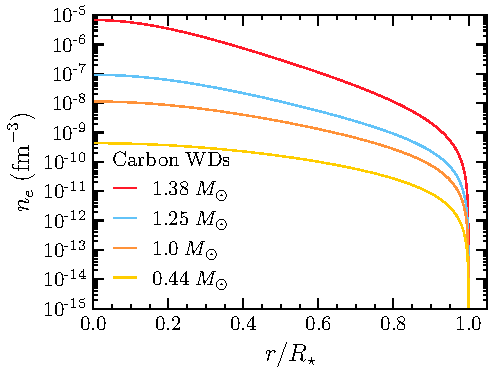
\includegraphics[width = 0.495\textwidth]{ne_prof.pdf}  
    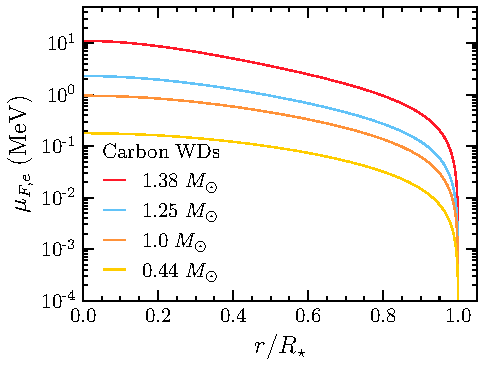
\includegraphics[width = 0.495\textwidth]{muFe_prof.pdf}  
    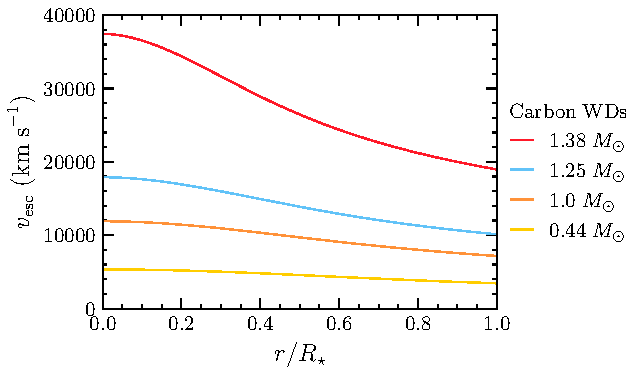
\includegraphics[width = 0.67\textwidth]{vesc_prof.pdf}
    \caption[Electron number density (top left), chemical potential (top right), and escape velocity (bottom) radial profiles for the carbon WDs with FMT EoS in Table~\ref{ch2:tab:WDs}.]{Electron number density (top left), chemical potential (top right), and escape velocity (bottom) radial profiles for the carbon WDs with FMT EoS in Table~\ref{ch2:tab:WDs}. The radial distance of each profile has been normalised to the radius of the star.}
    \label{ch2:fig:WDradprofs}
\end{figure}
%%%%%%%%%%%%%%%%%%%%%%%%%%%%%%%%%%%%%


The mass-radius relations obtained from a zero-temperature EoS begin to deviate from observations for low-mass WDs. 
To address this discrepancy, finite temperature effects can be introduced to the EoS~\cite{deCarvalho:2013rea_Relativisticfeynmanmetropolistellertreatment}. 
The extension to finite temperatures is made by reintroducing the temperature dependence in the Fermi-Dirac
distributions. Now, the electron chemical potential is no longer simply the Fermi energy of the system due to thermal corrections. Define the finite temperature Fermi-Dirac integrals of degree $s$ as
\begin{equation}
    F_s (\eta, \beta) = \int_0^\infty \frac{t^s\sqrt{1 + (\beta/2)t}}{1 + e^{t - \eta}}dt,
\end{equation}
where we define the dimensionless quantities 
\begin{align}
    t & = \frac{E_e - m_e}{\Tstar},\\
    \eta & = \frac{\varepsilon_{F,e}}{\Tstar},\\
    \beta & = \frac{\Tstar}{m_e},
\end{align}
for a star at temperature $\Tstar$. The Thomas-Fermi equilibrium condition within the WS cell is now given by 
\begin{equation}
    \varepsilon_{F,e}(r) - e V(r) = \Tstar \eta(r) - e V(r) = \mathrm{constant},
\end{equation}
with the Coulomb potential vanishing at the boundary of the cell as before. We now make the change of variables into the dimensionless quantities $\chi/r = \varepsilon_{F,e} / (\hbar c)$ and $x = x/x_\mathrm{WS}$ so that the Poisson equation~\ref{ch2:eq:poisson_WS_cell} becomes
\begin{align}
    \begin{split}
        \frac{d^2 \chi}{dx^2} &= -4 \pi \alpha_\mathrm{EM} x \left( \frac{3}{4\pi \Delta^3} \theta(x_c - x) \right.\\
        &\hspace{7em}\left. - \frac{\sqrt{2}}{\pi^2} \left( \frac{m_e}{m_\pi} \right)^2\left[ F_{1/2}(\eta, \beta) + \beta  F_{3/2}(\eta, \beta) \right] \right),
    \end{split}\\
    \eta(x) & = \left(\frac{1}{\lambda_\pi \Tstar}\right)\frac{\chi(x)}{x},
\end{align}
with the same boundary conditions as in Eq.~\ref{ch2:eq:TF_bc}.

The total energy of the cell remains very similar to the zero-temperature case, with the main differences being that it gains a contribution from the thermal motion of the nucleus, 
\begin{equation}
    E_\mathrm{th} = \frac{3}{2}\Tstar,
\end{equation} 
and that the electron energy density is now given by
\begin{equation}
    \mathcal{E}_e = m_e n_e + \frac{\sqrt{2}}{\pi^2} m_e^4 \beta^{5/2} \left[ F_{3/2}(\eta, \beta) + \beta F_{5/2}(\eta, \beta) \right].
\end{equation}
% 
The pressure of the cell will now gain contributions from the motion of the nucleus as well as the electron, such that the total pressure is
\begin{align}
    P_\mathrm{tot} & = P_N + P_e,\\
    P_N & = \frac{2}{3}\frac{E_\mathrm{th}}{V_\mathrm{WS}} = \frac{\Tstar}{V_\mathrm{WS}},\\
    P_e & = \frac{2^{3/2}}{3\pi} me^4 \beta^{5/2}\left[  F_{3/2}(\eta(x_\mathrm{WS}), \beta) + \beta F_{5/2}(\eta(x_\mathrm{WS}), \beta)  \right].
\end{align}
% 
In Fig.~\ref{ch2:fig:WD_mass_radius} we show the Mass-Radius relations obtained from the zero temperature FMT EoS together with several finite temperature configurations. As can be seen, the deviations from the zero temperature approximation begin at rather high temperatures, $\Tstar\gtrsim 10^7\K$, for masses $\lesssim 0.6 \Msun$. Additionally, we show a random selection of 20,000 WDs presented in the Gaia early data release 2 (EDR2) report~\cite{GentileFusillo_feb_GaiaDataRelease} as the yellow-red dots. The colour of the dot represents the internal temperature of the corresponding WD. The core temperature must be determined from the observed effective surface temperature of the star\footnote{The effective temperature is the temperature that characterises the surface of the star. Assuming that WDs are perfect blackbody emitters, the luminosity will be $L_\gamma = 4\pi \sigma_{SB} \, \Rstar^2 \, \Teff^4$, where $\sigma_{SB}$ is the Stefan–Boltzmann constant.}, with the relation between the two depending on the composition of the WD atmosphere. To obtain the central temperature from the reported effective temperatures, we use the WD cooling sequences generated in Ref.~\cite{Bedard_oct_Spectralevolutionhot}\footnote{The cooling sequence data can be obtained from \url{http://www.astro.umontreal.ca/~bergeron/CoolingModels}} assuming a thin hydrogen atmosphere. In general, there is good agreement between the mass-radius relations derived from the finite temperature FMT EoS and the observed internal temperatures of the WDs.

Given the non-linear nature of the differential equations that describe the FMT EoS (both at zero and finite temperatures), solving the system is a numerically challenging task. As there are no publically available resources to help solve these systems, a significant amount of time was put into solving this problem. The system is solved numerically using the non-linear shooting technique.

\begin{figure}[t!bp]
    \centering
    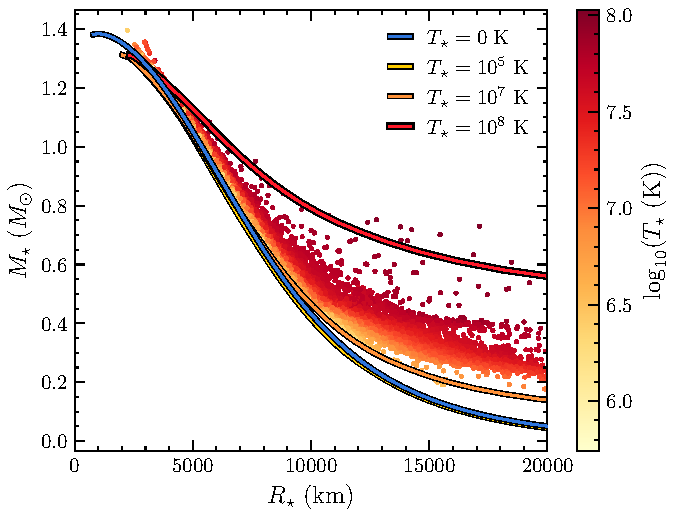
\includegraphics{WD_mass_radius.pdf}
    \caption[Mass-Radius relation of WDs calculated from the FMT EoS in the zero-temperature approximation (dark blue), at $10^{5}\K$ (yellow), $10^{7}\K$ (orange), and $10^{8}\K$ (red), together with observed WDs from Gaia EDR2 observations~\cite{GentileFusillo_feb_GaiaDataRelease} (yellow-red dots).]{Mass-Radius relation of WDs calculated from the FMT EoS in the zero-temperature approximation (dark blue), at $10^{5}\K$ (yellow), $10^{7}\K$ (orange), and $10^{8}\K$ (red), together with observed WDs from Gaia EDR2 observations~\cite{GentileFusillo_feb_GaiaDataRelease} (yellow-red dots). The colour of the dots represents the surface temperature of the WD inferred from cooling models~\cite{Bedard_oct_Spectralevolutionhot}.}
    \label{ch2:fig:WD_mass_radius}
\end{figure}
%%%%%%%%%%%%%%%%%%%%%%%%%%%%%%%%%%%%%


%%%%%%%%%%%%%%%%%%%%%%%%%%%%%%%%%%%%%
%%%%%%%%%%%%%%%%%%%%%%%%%%%%%%%%%%%%%
\subsection{Observational Status}
\label{ch2:subsec:WD_obs}
%%%%%%%%%%%%%%%%%%%%%%%%%%%%%%%%%%%%%
%%%%%%%%%%%%%%%%%%%%%%%%%%%%%%%%%%%%%

The rate at which the energy of the WD core is radiated away is determined by the outer non-degenerate layers of the atmosphere. 
Spectroscopic observations shed light on the composition of these layers and can be used to classify WDs in terms of $\sim$ six spectral types. 
Most of the observed WDs lie in the DA (hydrogen-rich) and DB (helium-rich) categories.  Note that as WDs slowly cool, they undergo spectral evolution. There is a well-defined relation between their luminosity and age (cooling time) that, together with recent breakthroughs in theory and observations, allow us to estimate the age of the stars within the solar neighbourhood and to date the nearest star clusters~\cite{Hansen:2004ih_HSTobservationswhite, Hansen:2007ve_Whitedwarfcooling, Bedin:2009it_jun_Endwhitedwarf, Hansen:2013gda_aug_Agedifferencetwo, Kilic_mar_Agesthindisk}. 

Over the past few decades, WDs have been extensively observed using photometry and spectroscopy. Most of the WDs have been discovered by large area surveys, such as the Sloan Digital Sky Survey (SDSS)~\cite{SDSS:2000hjo_Sloandigitalsky}. However, these local samples are dominated by young WDs with relatively high effective temperatures ($\Teff\gtrsim10^4\K$)~\cite{SDSS:2006iiz_Catalogspectroscopicallyconfirmed, Kleinman:2012nt_jan_SDSSDR7white, Tremblay_sep_Fieldwhitedwarf, Kepler_mar_Whitedwarfmass, Kepler_jun_Whitedwarfsubdwarf}. 
Recently, the local volume sample of nearby stars within $\sim100\pc$ has been catalogued by the Gaia spacecraft~\cite{Gaia:2018vmj_aug_Gaiadatarelease, Gaia:2020wqu_may_Gaiaearlydata}, an astrometric mission. New WD candidates have been identified~\cite{GentileFusillo_feb_GaiaDataRelease}, followed by dedicated spectroscopic observations~\cite{Tremblay_jul_Gaiawhitedwarfs,McCleery_jul_Gaiawhitedwarfs}, increasing the local sample of cool WDs ($\Teff\lesssim5000\K$). 

On the other hand, globular clusters (GCs) are the oldest known stellar systems in the Galaxy. Among them is Messier 4 (M4), also classified as NGC 6121, which is the closest globular cluster to Earth, being $\sim 1.9\kpc$ away ~\cite{Neeley_jul_Distanceglobularcluster, Watkins_apr_Tychogaiaastrometricsolution, Shao_nov_GaiaparallaxMilky}. 
The age of M4, $11.6\Gyr$, has been estimated using observations of faint cold WDs with the Hubble Space Telescope  (HST)~\cite{Hansen:2004ih_HSTobservationswhite, Bedin:2009it_jun_Endwhitedwarf}. 
This HST data, corrected for reddening and extinction, 
was converted into luminosities and effective temperatures in ref.~\cite{McCullough:2010ai_CaptureInelasticDark}. From these calculations, it is possible to infer WD radii and their corresponding masses by assuming a mass-radius relation. 


%%%%%%%%%%%%%%%%%%%%%%%%%%%%%%%%%%%%%
%%%%%%%%%%%%%%%%%%%%%%%%%%%%%%%%%%%%%
%%%%%%%%%%%%%%%%%%%%%%%%%%%%%%%%%%%%%
\section{Neutron Stars}
\label{ch2:sec:neutron_stars}
%%%%%%%%%%%%%%%%%%%%%%%%%%%%%%%%%%%%%
%%%%%%%%%%%%%%%%%%%%%%%%%%%%%%%%%%%%%
%%%%%%%%%%%%%%%%%%%%%%%%%%%%%%%%%%%%%

Being the end product of massive, $\gtrsim 8 \Msun$, stars, there are significantly fewer NSs than the WDs discussed above. As their name suggests, they are composed primarily of neutrons, which provide the degeneracy pressure required to prevent the gravitational collapse of the star.
The internal structure of an NS is significantly more complicated than that of a WD. Broadly speaking, an NS can be divided into five main regions. We give an overview of the important features of each of these regions and point the reader to Refs.~\cite{Glendenning_Compactstarsnuclear, Lattimer:2004pg_Physicsneutronstars, Haensel_NeutronstarsEqation, Weber:2007ch_may_NeutronStarInteriors, Camenzind_Compactobjectsastrophysics, Ozel:2015fia_Densematterequation,Ozel:2016oaf_jul_MassesRadiiEquation,Lattimer:2021emm_jul_NeutronStarsNuclear} for more in depth discussions. Working from the outside in, these regions are:

\subsubsection*{Atmosphere}
The atmosphere is an extremely thin layer of plasma that makes up less than 1\% of the NS mass. However, it plays an extremely important role as the observed spectrum radiation emitted by the star must pass through this region~\cite{Lattimer:2004pg_Physicsneutronstars, Haensel_NeutronstarsEqation}.

\subsubsection*{Outer Crust}
The outer crust is the thin layer of ionized Iron-56 nuclei that extends down until the density reaches the neutron drip point, $\rho_\star = \rho_\mathrm{ND} \sim 4.3\times 10^{11}\g\cm^{-3}$. This is the density at which neutrons begin to drip from the nuclei as their chemical potentials approach zero. The ionized electrons form a non-relativistic but degenerate gas, with their chemical potentials increasing as the density increases. This leads to the ``neutronisation'' of the nuclei as the beta-capture of electrons by protons increases.

\subsubsection*{Inner Crust}
The density within the inner crust spans the range between $\rho_\mathrm{ND}\lesssim \rho_\star \lesssim 0.5\rho_0$, with $\rho_0 \sim 2.8\times 10^{14}\g\cm^{-3}$ the nuclear saturation density (i.e. the density of nuclear matter)~\cite{Lattimer:2004pg_Physicsneutronstars, Haensel_NeutronstarsEqation, Grill:2014aea_Equationstatethickness}. Here, the neutrons that have dripped from the nuclei will potentially form a superfluid. Towards the crust-core boundary, the nuclear lattice begins taking on interesting topological structures that are distinguished by the configuration of the voids in the lattice. These are known as the so-called \textit{pasta phases}~\cite{Watanabe:2004tr_SimulationtransitionsPasta, Avancini:2010ch_Warmpastaphase, Yakovlev:2015vma_Electrontransportnuclear} of nuclear matter, which include 2D sheets (lasagne), cylindrical rods (spaghetti), or 3D clumps (gnocchi).
% \begin{itemize}
%     \item 2D void cylinders creating spaghetti structures of nuclei
%     \item Planar voids with slabs of nuclei forming lasagna sheets
%     \item 3D cylindrical voids leading to thin 2D cylinders of nuclear ziti
%     \item 3D spherical voids enclosed by ravioli
%     \item 2D circular voids in sheets of Swiss cheese
% \end{itemize}
Eventually, towards the crust-core interface, the nuclear matter transitions into a uniform medium\footnote{The nuclear minestrone, if you will.}. 

\subsubsection*{Outer Core}
Once densities go above $0.5\rho_0$, the nuclear clusters will dissolve into a homogeneous fluid that is composed of neutrons, protons, electrons, and muons known as $npeu$ matter. The relative abundances of the species, $Y_i=n_i/n_b$, are dictated by the conditions of electrical neutrality and beta-equilibrium.
Charge neutrality dictates that the abundances of the charged particles obeys
\begin{equation}
    Y_p = Y_e + Y_\mu,
\end{equation}
while beta-equilibrium refers to the balance between the weak decays of neutrons and the electron/muon capture by the protons,
\begin{gather}
    n \rightarrow p + \ell^- +\bar{\nu}_\ell,\label{ch2:eq:beta_decay}\\
    p + \ell^- \rightarrow n + \nu_\ell,\label{ch2:eq:electron_capture}
\end{gather}
with $\ell = e, \mu$. Muons will begin to replace electrons in these reactions once the electron chemical potential exceeds the mass of the muon, $\mu_{F,e} \gtrsim m_\mu = 105.7\MeV$. As neutrinos are assumed to escape the NS once produced, the relation between the chemical potential of the leptons is simply
\begin{equation}
    \mu_{F,e} = \mu_{F,\mu}.
\end{equation}
The outer core region ends once the density reaches $\rho_\star \sim 2\rho_0$, and we transition into the inner core.

\subsubsection*{Inner Core}
The densities within the inner cores of NSs extend between $2\rho_0 \lesssim \rho_\star \lesssim (10-15)\rho_0$ and are hence a mystery to this day. As the density greatly exceeds any material that can be produced in a laboratory, the exact composition of this region is unknown and depends on the equation of state one adopts to describe it. Some of the more well-known candidates are
\begin{itemize}
    \item A hyperonic matter component, i.e. nucleons containing a valence strange quark. These appear once the neutron chemical potential equals that of the $\Lambda^0$ hyperon, with the $\Xi^-$ appearing once its chemical potential equals the sum of the chemical potentials of the neutrons and electrons~\cite{Weber:2007ch_may_NeutronStarInteriors, Fortin:2014mya_Neutronstarshyperon}. 
    \item Pion/Kaon condensates. These are Bose-Einstein condensates of pion/kaon-like excitations~\cite{Baym:1973zk_Pioncondensationnuclear,Baym:1974vzp_Pioncondensationneutron,Kaplan:1986yq_StrangeGoingsDense, Ellis:1995kz_Kaoncondensationneutron, Brown:1992ib_Novelmechanismkaon, Ma:2022fmu_jan_Kaonmesoncondensate}. 
    \item A quark-gluon plasma comprised of deconfined $u,\; d$ and $s$ quarks and gluons~\cite{Akmal:1998cf_Equationstatenucleon,Baym:2006rq_Neutronstarsquark,Baym:2017whm_Hadronsquarksneutron}.
\end{itemize}


%%%%%%%%%%%%%%%%%%%%%%%%%%%%%%%%%%%%%
%%%%%%%%%%%%%%%%%%%%%%%%%%%%%%%%%%%%%
\subsection{Observational Status}
\label{ch2:subsec:NS_obs}
%%%%%%%%%%%%%%%%%%%%%%%%%%%%%%%%%%%%%
%%%%%%%%%%%%%%%%%%%%%%%%%%%%%%%%%%%%%

Unlike the WDs discussed above, there are significantly fewer NS observations to constrain the EoS. However, recent years have seen significant strides in furthering our understanding of matter at super-nuclear densities, both from a theory and observational standpoint. On the theoretical side, these advances come from developments in chiral EFT, allowing more detailed modelling of nuclear interactions~\cite{Hebeler:2009iv_Chiralthreenucleonforces, Tews:2012fj_jan_NeutronMatterNexttoNexttoNexttoLeading, Tews:2018kmu_jun_Constrainingspeedsound}. The observational data has been bolstered thanks to the onset of gravitational wave astronomy due to the LIGO-VIRGO experiment~\cite{LIGOScientific:2017zic_Gravitationalwavesgammarays, LIGOScientific:2018cki_oct_GW170817MeasurementsNeutron, LIGOScientific:2018hze_Propertiesbinaryneutron} and the launch of the Neutron star Interior Composition Explorer (NICER) X-ray timing instrument. 

Ultimately, what is needed to further constrain the NS EoS are more precise observations of NS masses and radii, which can be obtained from various observational techniques. NS masses have historically been much easier to measure than their radii. In particular, masses of NSs in binary systems can be precisely determined as the underlying gravitational theories are well-understood today~\cite{Steiner:2010fz_Equationstateobserved, Lattimer:2013hma_Neutronstarmasses, Ozel:2015fia_Densematterequation, Ozel:2016oaf_jul_MassesRadiiEquation, Miller:2016pom_Observationalconstraintsneutron}. The radii must be determined by assuming the NSs emit a blackbody spectrum. However, this method is only reliable for cool NSs where the atmospheric models are well understood~\cite{Miller:2016pom_Observationalconstraintsneutron}. 

The NICER experiment can provide much more precise measurements of NS radii than previous methods. This is achieved by measuring the X-ray pulse profiles of pulsars that are sensitive to how light bends around the star. This provides information on the compactness of the star, $G M_\star/R_\star c^2$, that can be used to determine $M_\star$ and $R_\star$ given that the mass can usually be determined through other means. The heaviest NS observed to date, the millisecond pulsar PSR J0740+6620~\cite{Miller:2021qha_sep_RadiusPSRJ0740, Riley:2021pdl_sep_NICERViewMassive}, had its mass determined by measuring the relativistic Shapiro time delay~\cite{Shapiro:1964uw_FourthTestGeneral}\footnote{This refers to the time it takes for light to move out of a gravitational well taking longer than the naive Newtonian prediction due to the curvature of space-time.} of the radio signal, allowing the radius to be obtained once the compactness was measured~\cite{NANOGrav:2019jur_sep_RelativisticShapirodelay}. Refined analyses result in a mass of 2.08$\pm$0.07$\Msun$~\cite{Fonseca:2021wxt_jul_RefinedMassGeometric} and a radius of $12.39^{+1.30}_{-0.98} \km$~\cite{Riley:2021pdl_sep_NICERViewMassive} or $13.71^{+2.61}_{-1.50} \km$~\cite{Miller:2021qha_sep_RadiusPSRJ0740} at 68\% confidence levels. 


Gravitational wave astronomy offers an alternative and independent determination of NS masses and radii to the electromagnetic observations above. The best candidate events for this analysis are NS binary mergers, though these are expected to be an uncommon occurrence. As the NSs inspiral toward each other, they will begin to deform due to the tidal forces they induce on one another~\cite{Lattimer:2019eez_jun_NeutronStarMass}. 
This deformation will alter the waveform observed at the detectors, with the shift in the phase of the waveform depending on the mass ratio, $q = M_2/M_1 <1$, the chirp mass of the system, $\mathcal{M}_\mathrm{chirp} = (M_1 M_2)^{3/5}/(M_1 + M_2)^{1/5}$, and a combination of the tidal deformabilities, $\tilde\Lambda$. The latter refers to how susceptible the star is to deformation due to tidal forces acting upon it, with larger values corresponding to less compact objects. Comparing the observed waveform to that determined from precise numerical simulations allows constraints to be placed on these parameters and, ultimately, on the masses and radii of the merging NSs.

Furthermore, the electromagnetic emission from the remnant object provides information about the maximum mass an NS can achieve. 
If the mass of the remnant object is too large, it will collapse into a black hole, and it is highly unlikely that a gamma-ray burst will occur. If the remnant does not immediately collapse, then its mass and how it is rotating determines whether it will be hydrodynamically stable, unstable, or metastable against gravitational collapse. A remnant that undergoes differential rotation\footnote{This is when components of the star at different latitudes have different angular velocities.} can support heavier masses than one that is uniformly rotating. Hence, the afterglow spectrum can inform us as to how the star is rotating. Comparing the maximum mass supported by this rotation to the initial mass after inspiral yields an upper bound on the maximum NS mass achievable. 

To date, the only confirmed NS-NS merger is the merger event GW170817 observed at LIGO-VIRGO in 2017~\cite{LIGOScientific:2018cki_oct_GW170817MeasurementsNeutron, LIGOScientific:2018hze_Propertiesbinaryneutron}, with the gamma-ray burst counterpart signal observed at the Fermi Gamma-ray Burst Monitor and INTEGRAL satellite~\cite{LIGOScientific:2017zic_Gravitationalwavesgammarays}. These observations led to the constraint that the radius of a $1.4\Msun$ NS has an upper bound of $R_{1.4} < 13.3\km$~\cite{LIGOScientific:2018cki_oct_GW170817MeasurementsNeutron, De:2018uhw_aug_TidalDeformabilitiesRadii}, and that the maximum NS mass must be $M_\mathrm{NS}^\mathrm{MAX} < 2.18\Msun$~\cite{LIGOScientific:2017zic_Gravitationalwavesgammarays}. These constraints on the neutron star mass-radius relation are shown as the shaded turquoise and red regions of Fig~\ref{ch2:fig:NS_mass_rad}. 

%%%%%%%%%%%%%%%%%%%%%%%%%%%%%%%%%%%%%
\begin{figure}[t!bp]
    \centering
    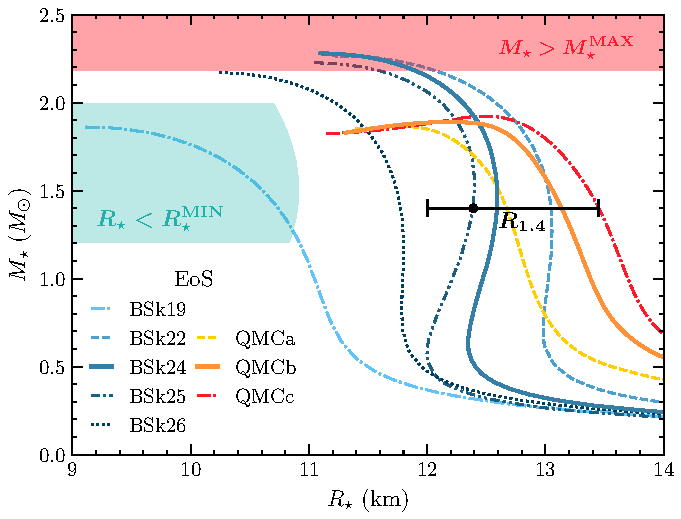
\includegraphics{NS_mass_radius.pdf}
    \caption[Neutron Star Mass-Radius relation predicted by the BSk (blue lines) and QMC (red lines) EoSs.]{Neutron Star Mass-Radius relation predicted by the BSk (blue lines) and QMC (red lines) EoSs. Constraints obtained from the gravitational wave event GW170817 are shown as the shaded regions, with the lower bound on the radius in turquoise and the maximum NS mass possible in red. The line band labelled $R_{1.4}$ indicates the constraints on the radius of a $1.4\;\Msun$ NS.}
    \label{ch2:fig:NS_mass_rad}
\end{figure}
%%%%%%%%%%%%%%%%%%%%%%%%%%%%%%%%%%%%%



%%%%%%%%%%%%%%%%%%%%%%%%%%%%%%%%%%%%%
%%%%%%%%%%%%%%%%%%%%%%%%%%%%%%%%%%%%%
\subsection{Neutron Star Equations of State}
\label{ch2:subsec:NS_EoS}
%%%%%%%%%%%%%%%%%%%%%%%%%%%%%%%%%%%%%
%%%%%%%%%%%%%%%%%%%%%%%%%%%%%%%%%%%%%

Given the scarce constraints placed on the NS mass-radius relation, the literature contains numerous equations of state that can be used to incorporate the internal structure into our calculations. In this work, we adopt two different EoSs, which we detail here. 

\subsubsection{The Brussels-Montreal EoS}
The first family of EoSs adopted in this work are based on the Brussels-Montreal (BSk) energy density functionals~\cite{Chamel:2009yx_FurtherexplorationsSkyrmeHartreeFockBogoliubov, Goriely:2010bm_FurtherexplorationsSkyrmeHartreeFockBogoliubov, Pearson:2011zz_jun_Propertiesoutercrust, Pearson:2012hz_Innercrustneutron, Potekhin:2013qqa_Analyticalrepresentationsunified, Pearson:2018tkr_Unifiedequationsstate}, for cold, non-accreting NSs. In these models, the density-dependent nucleon interactions are accounted for via a mean-field approximation in either the Hartree-Fock (HF) or Hartree-Fock-Bogoliubov (HFB) formalism\footnote{The HF method accounts for the energy associated with nucleon pairings, while the HFB method neglects this contribution.}, through effective Skyrme type forces~\cite{Bender:2003jk_Selfconsistentmeanfieldmodels, Stone:2006fn_Skyrmeinteractionfinite}. The BSk EoS family are unified EoSs, meaning they describe all the regions of the NS interior using the single effective Hamiltonian. Furthermore, the authors provide public \texttt{FORTRAN} subroutines that implement fits to the EoS quantities, such as the pressure and density as functions of the baryon number density, allowing straightforward implementation of the EoS. 

The authors provide these fits to eight configurations of the BSk EoS, labelled BSk19-26. Of these, the older BSk19-21  functionals were fitted to older atomic mass data that has since been updated in the newer models, BSk22-26. The mass-radius relation predicted by a selection of these models is shown in Fig.~\ref{ch2:fig:NS_mass_rad} by the blue lines. Missing are the BSk20 and 21 models, as they give very similar results to the 26 and 24 models, respectively. The BSk19 EoS is partially ruled out from the lower bound on NS radii obtained from the electromagnetic counterpart of the GW170817 event~\cite{Koppel:2019pys_Generalrelativisticdeterminationthreshold}, while BSk22 is ruled out from constraints on the tidal deformability from the same event~\cite{Perot:2019gwl_Rolesymmetryenergy}. Additionally, BSk22 does not support the presence of direct Urca\footnote{This is another name given to the reactions in Eqs.~\ref{ch2:eq:beta_decay},~\ref{ch2:eq:electron_capture}.} processes in NSs described by this EoS. These processes are required to explain observations of a small population of NSs that have cooled to temperatures below those predicted by the ``minimal cooling paradigm''~\cite{Gusakov:2004se_Enhancedcoolingneutron, Page:2004fy_MinimalCoolingNeutron}. On the other hand, the BSk26 functional predicts that all stable NSs will support direct Urca processes. This goes against the current observational evidence that a majority of NSs are well-modelled by the minimal cooling paradigm, ruling the EoS out. Of the remaining two models, BSk24 and 25, we choose to adopt BSk24 as it gives slightly better fits to NS mass data than that of BSk25. 

We use the BSk24 EoS to generate four benchmark NSs with masses of $1$, 1.5, 1.9 and 2.16$\Msun$, with the central density $\rho_c$, stellar mass, radius, metric factor $B(\Rstar)$ and central speed of sound $c_s(0)$ in Table~\ref{ch2:tab:BSk_configs}. 
Radial profiles of the baryon number density $n_b(r)$, metric factor $B(r)$, neutron chemical potential $\kinFn(r)$, and neutron abundance $Y_n(r)$, are shown in Fig.~\ref{ch2:fig:BSk_profiles}. 



%%%%%%%%%%%%%%%%%%%%%%%%%%%%%%%%%%%%%%%%
\begin{table}[tb]
    \centering
    \begin{tabular}{l c c c c}
    \toprule
     EoS &  BSk24-1 &  BSk24-2 &  BSk24-3 &  BSk24-4 \\ \midrule\midrule
    $\rho_c$ $[\rm{g \, cm^{-3}}]$ & $5.94 \times 10^{14}$   & $7.76 \times 10^{14}$ & $1.04 \times 10^{15}$ & $1.42 \times 10^{15}$  \\
    $\Mstar$ $[\Msun]$ & 1.000 & 1.500 & 1.900 & 2.160  \\
    $\Rstar$ [km] & 12.215  & 12.593 & 12.419 & 11.965 \\
    $B(\Rstar)$ & 0.763 & 0.648 & 0.548 & 0.467\\
    $c_s(0)$ $[c]$ & 0.511 & 0.628 & 0.734 & 0.835 \\
    \bottomrule
    \end{tabular} 
    \caption[Benchmark NSs, for four different configurations of the equations of state (EoS) for cold non-accreting neutron stars with Brussels–Montreal functionals BSk24 \cite{Pearson:2018tkr_Unifiedequationsstate}.]{Benchmark NSs, for four different configurations of the equations of state (EoS) for cold non-accreting neutron stars with Brussels–Montreal functionals BSk24 \cite{Pearson:2018tkr_Unifiedequationsstate}. EoS configurations are determined by the central mass-energy density $\rho_c$.}
    \label{ch2:tab:BSk_configs}
\end{table} 
%%%%%%%%%%%%%%%%%%%%%%%%%%%%%%%%%%%%%%%%

%%%%%%%%%%%%%%%%%%%%%%%%%%%%%%%%%%%%%
\begin{figure}[t!bp]
    \centering
    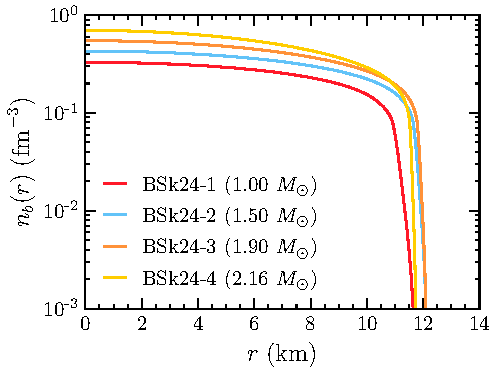
\includegraphics[width=0.495\textwidth]{nb_BSk_prof.pdf}
    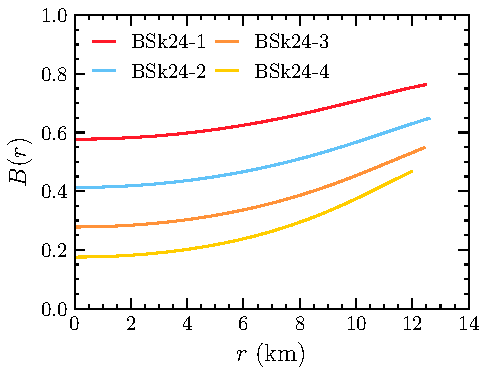
\includegraphics[width=0.495\textwidth]{B_BSk_prof.pdf}
    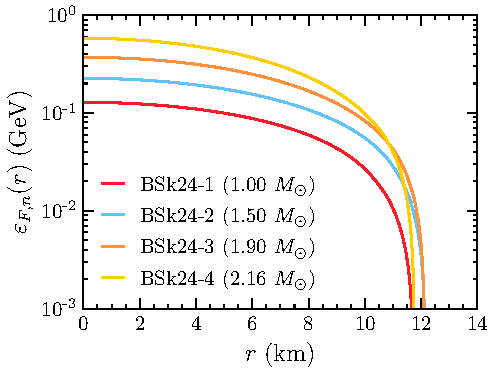
\includegraphics[width=0.495\textwidth]{epsFn_BSk_prof.pdf}
    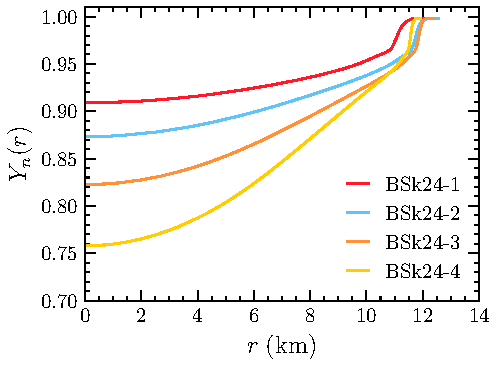
\includegraphics[width=0.495\textwidth]{Yn_BSk_prof.pdf}
    \caption[Radial profiles of the baryon number density (top left), metric factor $B(r)$ (top right), neutron chemical potential (bottom left), and neutron abundance (bottom right) for the four benchmark NS of the BSk24 EoS in Table~\ref{ch2:tab:BSk_configs}.]{Radial profiles of the baryon number density (top left), metric factor $B(r)$ (top right), neutron chemical potential (bottom left), and neutron abundance (bottom right) for the four benchmark NS of the BSk24 EoS in Table~\ref{ch2:tab:BSk_configs}.}
    \label{ch2:fig:BSk_profiles}
\end{figure}
%%%%%%%%%%%%%%%%%%%%%%%%%%%%%%%%%%%%%
    

While BSk24 and 25 lie well within current observational constraints, they are minimal models in that they only account for $npe\mu$ matter and do not incorporate any exotic species within the NS core. This is problematic as it is highly likely that hyperonic matter will appear in the cores of NS heavier than $\sim 1.7\;\Msun$.  Additionally, the Skyrme forces that describe the nuclear interaction are treated as being non-relativistic, while the nucleons in heavier stars can become semi-relativistic. To address these concerns, later works~\cite{Anzuini:2021lnv_nov_Improvedtreatmentdark, Bell:2023ysh_dec_ThermalizationAnnihilationDark} adopted the Quark-Meson Coupling (QMC) EoS.



\subsubsection*{The Quark-Meson Coupling EoS}

The second EoS adopted is based on the QMC model of Refs.~\cite{Guichon:1987jp_Possiblequarkmechanism, Guichon:1995ue_Rolenucleonstructure, Saito:2005rv_Nucleonhadronstructure, Guichon:2018uew_QuarkMesonCouplingQMC}, in which baryons are described as bags of three valence quarks, with the bags themselves modelled by the MIT bag model~\cite{Chodos:1974pn_Baryonstructurebag}. The interactions among the baryons are described by the exchange of mesons between the valence non-strange quarks and are formulated within a relativistic mean-field Lagrangian. The exchange of the vector mesons acts as an overall shift to the energy of the baryons\footnote{A simple analogy for this is how the force of an electron in an electromagnetic field is due to the exchange of photons, which are vector fields. The total energy of the electron is a shift relative to the free electron energy.}. The scalar mean fields play a significantly more important role, modifying the effective mass of the baryons. The scalar (and also vector) couplings are density-dependent, leading to an effective mass of the baryons that varies throughout the NS. The density dependence of these couplings is equivalent to including repulsive three-body forces between the baryons and arises naturally in the QMC model through the in-medium modification of the baryonic structure~\cite{Guichon:2004xg_Quarkstructurenuclear, Thomas:2021kio_jul_Rolequarksnuclear}. Additional details on the energy density and couplings of the QMC model adopted in this work are given in Appendix~\ref{appendix:QMC_details}.

The mass-radius relation for three different configurations of the QMC EoS, namely three different choices of the isovector coupling constant, is shown as the red lines in Fig.~\ref{ch2:fig:NS_mass_rad}, obtained from Ref.~\cite{Motta:2019tjc_Isovectoreffectsneutron}. Of these, QMCb (orange solid line in Fig.~\ref{ch2:fig:NS_mass_rad}) lies within the constraints on the radius of a $1.4\;\Msun$ NS from GW170817 and can produce an NS of mass $1.908 \pm 0.016\;\Msun$, the currently preferred mass of PSR J1614-2230 obtained by the NANOGrav collaboration~\cite{NANOGrav:2017wvv_apr_NANOGrav11yearData}\footnote{As mentioned above, the current heaviest NS has a mass of $2.08\pm 0.07\Msun$ though the implications of this on the QMC EoS are beyond the scope of this work.}.

The QMCb EoS data was provided by the authors of Ref.~\cite{Motta:2019tjc_Isovectoreffectsneutron} for use in this work and will be referred to as simply the QMC EoS from here on. From this, we calculate the internal structure of four benchmark QMC NSs, similar to the BSk models of Table~\ref{ch2:tab:BSk_configs}, with the central baryon density replacing the central density and the speed of sound omitted. The relevant parameters are shown in Table~\ref{ch2:tab:QMC_configs}. The top four plots in Fig.~\ref{ch2:fig:QMC_profiles} show the radial profiles for the number densities of the neutrons and protons for each configuration on the left, with their effective masses shown on the right. The bottom two plots of the same figure show the number densities for each species within the heaviest star on the left, including leptons in dashed lines, with the effective masses for each of the baryons on the right. The replacement of high-momentum neutrons with low-momentum hyperons is clearly seen in the bottom left plot as the neutron number density dips towards the centre of the massive star. As the densities are high enough for the charged hyperon $\Xi^-$ to appear, the abundance of leptons decreases due to the requirement of charge neutrality, also seen in this plot. 

%%%%%%%%%%%%%%%%%%%%%%%%%%%%%%%%%%%%%
\begin{table}[t!bp]
    \centering
    \begin{tabular}{l c c c c}
    \toprule
     EoS &  QMC-1 &  QMC-2 &  QMC-3 &  QMC-4 \\ \midrule\midrule
    $n_{\cal B}^c$ $[\fm^{-3}]$ & 0.325 & 0.447 & 0.540 & 0.872\\
    $\Mstar$ $[\Msun]$ & 1.000 & 1.500 & 1.750 & 1.900  \\
    $\Rstar$ [km] &  13.044 & 12.847 & 12.611 & 12.109 \\
    $B(\Rstar)$ & 0.772 & 0.653 & 0.588 & 0.535\\
    \bottomrule
    \end{tabular} 
    \caption[Benchmark NSs for four different configurations of the QMC equation of state.]{Benchmark NSs for four different configurations of the QMC equation of state. 
    EoS configurations are determined by the central number density $n_{\cal B}^c$.
    }
    \label{ch2:tab:QMC_configs}
\end{table} 
%%%%%%%%%%%%%%%%%%%%%%%%%%%%%%%%%%%%%

%%%%%%%%%%%%%%%%%%%%%%%%%%%%%%%%%%%%%
\begin{figure}[t!bp]
    \centering
    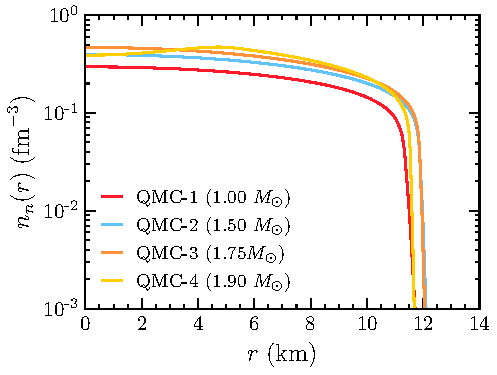
\includegraphics[width=0.495\textwidth]{nn_QMC_profs.pdf}
    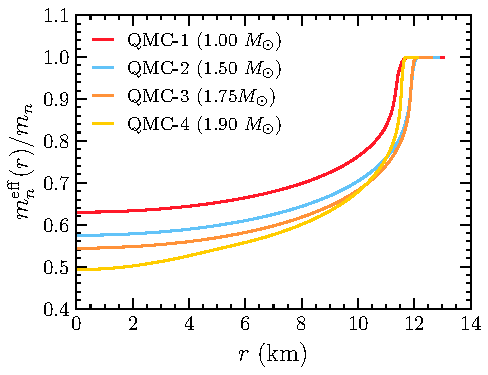
\includegraphics[width=0.495\textwidth]{meff_n_QMC_profs.pdf}
    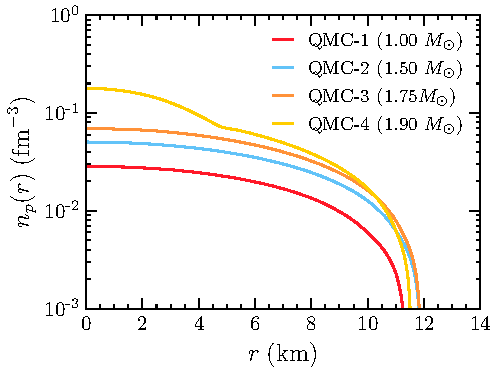
\includegraphics[width=0.495\textwidth]{np_QMC_profs.pdf}
    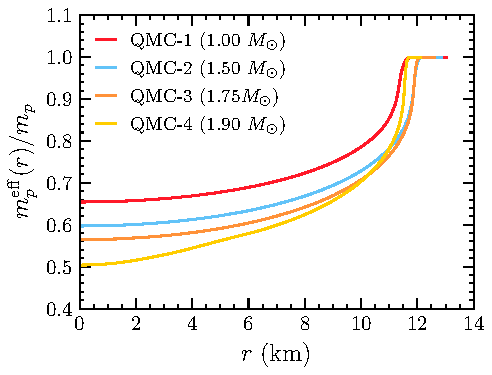
\includegraphics[width=0.495\textwidth]{meff_p_QMC_profs.pdf}
    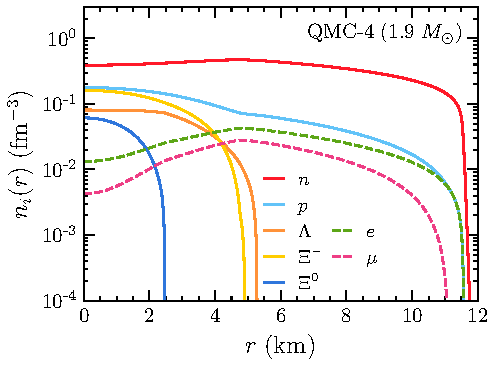
\includegraphics[width=0.495\textwidth]{ni_QMC_profs.pdf}
    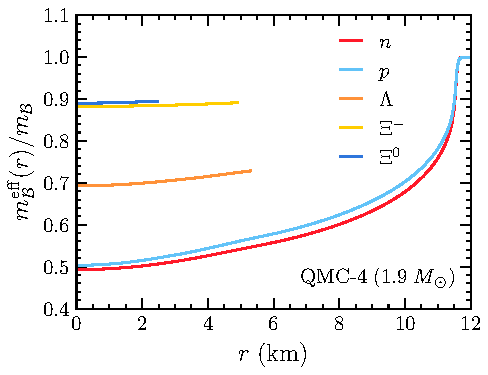
\includegraphics[width=0.495\textwidth]{meff_B_QMC_profs.pdf}
    \caption[Number density profiles (left) and the ratio of the effective mass to the bare mass (right) for neutrons (top) and protons (middle) for benchmark configurations of the QMC EoS in Table~\ref{ch2:tab:QMC_configs}.]{Number density profiles (left) and the ratio of the effective mass to the bare mass (right) for neutrons (top) and protons (middle) for benchmark configurations of the QMC EoS in Table~\ref{ch2:tab:QMC_configs}. In the bottom panels, we show the same profiles for all species in the heaviest NS considered, QMC-4, which contains hyperonic matter.}
    \label{ch2:fig:QMC_profiles}
\end{figure}
%%%%%%%%%%%%%%%%%%%%%%%%%%%%%%%%%%%%%


  %% Capture formalism
  \graphicspath{{img/capture_intro/}}
%%%%%%%%%%%%%%%%%%%%%%%%%%%%%%%%%%%%%
%%%%%%%%%%%%%%%%%%%%%%%%%%%%%%%%%%%%%
%%%%%%%%%%%%%%%%%%%%%%%%%%%%%%%%%%%%%

\chapter{Improved Treatment of Dark Matter Capture in Compact Objects}
\label{chapter:capture_intro}

\begin{synopsis}
This chapter combines aspects of Refs.~\cite{Bell:2020jou_sep_ImprovedTreatmentDark,Bell:2020lmm_mar_ImprovedTreatmentDark,Anzuini:2021lnv_nov_Improvedtreatmentdark} to give a complete introduction to the formalism we have built for dark matter capture in compact objects. We begin by reviewing aspects of Gould's formalism for capture in the Sun~\cite{Gould:1987ir_ResonantEnhancementsWIMP,Gould:1987ju_WeaklyInteractingMassive}. We then build upon these results to incorporate relativistic corrections and the effects of Pauli Blocking due to scattering from a degenerate media in a self-consistent manner. Important aspects of both the interaction and capture rates are discussed, including Pauli blocking for low mass DM and the effects of multiple scatting in the high-mass regime. We then apply our results to the example DM scattering from neutron targets using the BSk24 EoS to model the neutron star.
\end{synopsis}
%%%%%%%%%%%%%%%%%%%%%%%%%%%%%%%%%%%%%
%%%%%%%%%%%%%%%%%%%%%%%%%%%%%%%%%%%%%
%%%%%%%%%%%%%%%%%%%%%%%%%%%%%%%%%%%%%



%%%%%%%%%%%%%%%%%%%%%%%%%%%%%%%%%%%%%
%%%%%%%%%%%%%%%%%%%%%%%%%%%%%%%%%%%%%
%%%%%%%%%%%%%%%%%%%%%%%%%%%%%%%%%%%%%
\section{Dark Matter Capture in the Sun}
\label{ch3:sec:solar_capture_full}
%%%%%%%%%%%%%%%%%%%%%%%%%%%%%%%%%%%%%
%%%%%%%%%%%%%%%%%%%%%%%%%%%%%%%%%%%%%
%%%%%%%%%%%%%%%%%%%%%%%%%%%%%%%%%%%%%

Before jumping into the capture formalism relevant to compact objects, it will serve us well to review the formalism laid out by Gould for capture in the Sun~\cite{Gould:1987ju_WeaklyInteractingMassive, Gould:1987ir_ResonantEnhancementsWIMP}. 

To begin, we consider the flux of dark matter particles that pass through a spherical shell a large distance $R$ from the star, where the gravitational field is negligible. For this, we need to know the distribution function of the relative velocity between the DM and the stellar constituents. 
The velocity distribution function will be spatially isotropic, and so for simplicity we will assume that the DM follows a Maxwell-Boltzmann distribution function, 
\begin{equation}
    f_\infty(\tilde{u}_\chi) d\tilde{u}_\chi= 4 \pi \left( \frac{3}{2 \pi} \right)^{3/2}\frac{\tilde{u}_\chi^2}{v_d^2} \exp\left(-\frac{3 \tilde u_\chi^2}{2 v_d^3}\right)\,d\tilde u_\chi, 
\end{equation}
where $\tilde u_\chi$ is the DM velocity in the halo, and $v_d$ is the DM halo velocity dispersion.

Taking into account the motion of the star through the halo and the thermal motion of the constituents, which are assumed to follow a Maxwell-Boltzmann distribution, gives the relative velocity between the DM and targets, $ u_\chi$. 
The distribution function for the relative velocity can be expressed as~\cite{Busoni:2017mhe_oct_Evaporationscatteringmomentum}
\begin{equation}
    f_{\mathrm{MB}}(u_\chi, \Tstar)du_\chi = \frac{u_\chi}{v_\star} \sqrt{\frac{3 }{2 \pi (v_d^2 + 3 T_\star /\mi)}} \left( e^{-\frac{3(u_\chi - v_\star)^2}{2(v_d^2 + 3 T_\star /\mi)}} - e^{-\frac{3(u_\chi + v_\star)^2}{2(v_d^2 + 3 T_\star /\mi)}} \right)du_\chi,
    \label{ch3:eq:MB_finit_T}
\end{equation}
where $v_\star$ is the star's velocity in the halo rest frame\footnote{This is the frame where the DM has an average velocity of zero.}, $T_\star$ is the temperature of the star, and $\mi$ is the mass of the target.

Returning to the large spherical shell of radius $R$, given the velocity distribution function, we can obtain the flux of DM through this surface. The rate of DM particles passing through a surface element $d\tilde{A}$ with velocity between $u_\chi$ and $u_\chi + du_\chi$, with an angle to the normal of $d\tilde{A}$ between $\tilde\theta$ and $\tilde \theta + d\tilde \theta$ and an azimuthal angle between $\tilde \phi$ and $\tilde \phi + d\tilde \phi$ is given by~\cite{Press:1985ug_Capturesungalactic}
\begin{align}
    \frac{dN_\chi}{dt} &= \frac{\rho_\chi}{m_\chi}f_{\mathrm{MB}}(u_\chi, \Tstar) \vec{u}\cdot d\vec{\tilde{A}}\, d u_\chi\, \frac{d\tilde \Omega}{4\pi}\\
    & = \frac{\rho_\chi}{m_\chi}\fMB(u_\chi, \Tstar)u_\chi \cos\tilde\theta \,d\tilde{A}\, d u_\chi\,  \frac{d\cos\tilde\theta \,d\tilde\phi}{4\pi}\\
    & = \frac{1}{4}\frac{\rho_\chi}{m_\chi}\fMB(u_\chi, \Tstar)u_\chi d\tilde{A}\, d u_\chi\,d\cos^2\tilde\theta,
\end{align}
where we have integrated over the azimuthal angle $\tilde \phi$ due to the isotropy of the system. The number density of the DM is included through the $\rho_\chi/m_\chi$ factor. 
Integrating over the area of the sphere is trivial due to isotropy, leaving us with 
\begin{align}
    \frac{dN_\chi}{dt} &= \pi \frac{\rho_\chi}{m_\chi} f(u_\chi, \Tstar)u_\chi\, d u_\chi \, d\cos^2\tilde\theta,
\end{align}
with the integration interval for $\cos^2\tilde\theta$ being $(0, 1)$.

As the DM begins to infall from this large distance $R$ to a closer distance $r$, the star's gravitational field will boost the velocity by the local escape velocity $v_e(r)$ such that
\begin{align}
    w^2_\chi(r) &= u^2_\chi + v_e^2(r),\\
    v_e^2(r) & = \frac{2 G M_\star}{R_\star} + \int_r^{R_\star} \frac{G M_\star(r')}{r'^2}\,dr'.
\end{align}
Due to the conservation of angular momentum, we can relate the angular momentum of the DM at the two distances $R$ and $r$ such that
\begin{equation}
    J_\chi = m_\chi R u_\chi \sin \tilde\theta = m_\chi r w_\chi(r) \sin\theta \leq m_\chi r w_\chi(r) \equiv J_{\mathrm{max}},
\end{equation}
where $\theta$ is the incident angle of the DM at the closer distance $r$, and we have defined the maximum angular momentum $J_{\mathrm{max}}$ corresponding to a linear DM trajectory.

Changing integration variables from $\cos^2\tilde \theta$ to $J_\chi$ allows us to write the number of DM particles passing through the shell per unit volume as
\begin{equation}
    \frac{dN_\chi}{dt} = 2\pi \frac{\rho_\chi}{m_\chi} \frac{\fMB(u_\chi, \Tstar)}{u_\chi} r^2 w_\chi^2(r) \frac{J_\chi dJ_\chi}{J^2_\mathrm{max}}\,du_\chi.\label{ch3:eq:shell_flux}
\end{equation}
The geometry of the system is shown in Fig.~\ref{ch3:fig:capturegeometry} for clarity.

\begin{figure}
    \centering
    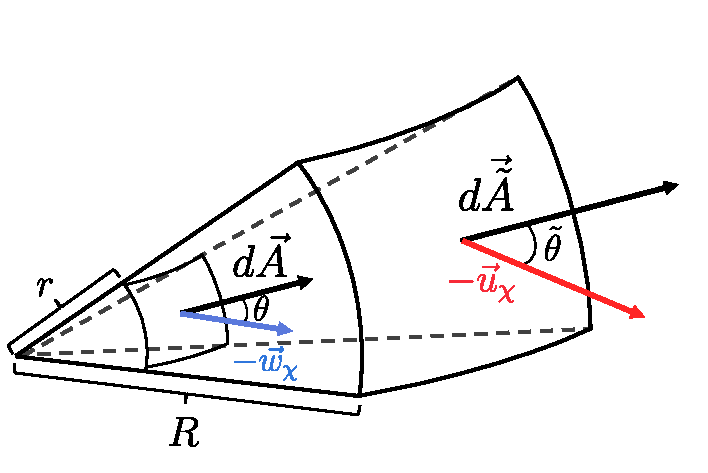
\includegraphics{capture_geometry.pdf}
    \caption{Geometry of the capture process, showing two elements of spheres with radii, $r$ and $R$, near and far from the star respectively.}
    \label{ch3:fig:capturegeometry}
\end{figure}

The probability that the DM interacts with the constituents of the shell depends on the interaction rate, $\Omega(w_\chi)$, multiplied by the time spent in the shell, $dt = dr/\dot r$. Hence, the probability of scattering within the shell is
\begin{equation}
    \Omega(w_\chi) \frac{dr}{\dot r} = 2  \Omega(w_\chi)\frac{1}{w_\chi}\left(1 - \left(\frac{J_\chi}{r w_\chi}\right)^2 \right)^{-1/2} \Theta(J_{\mathrm{max}} - J_\chi)\,dr,\label{ch3:eq:int_prob_1}
\end{equation}
where the factor of 2 is due to the DM having two opportunities to pass through the shell, once when incoming and another after turning around\footnote{The radial velocity $\dot r$ is a standard result in orbital mechanics and can be obtained from the central force Lagrangian.}. The step-function is put in to ensure the angular momentum does not exceed its maximum allowed value. 

For a scattered DM to be considered captured, it must lose enough energy in the collision to become gravitationally bound. The rate at which a DM particle scatters from an initial velocity $w_\chi$ to a final velocity $v<v_e(r)$ is given by~\cite{Gould:1987ju_WeaklyInteractingMassive, Gould:1987ir_ResonantEnhancementsWIMP, Busoni:2017mhe_oct_Evaporationscatteringmomentum}
\begin{align}
    \Omega^{-}(w_\chi) &= \int_0^{v_e} R^-(w_\chi \rightarrow v) dv,\label{ch3:eq:down_rate_1}\\
    R^-(w_\chi \rightarrow v) & = \int n_T(r) \frac{d\sigma_{\chi T}}{dv} |\vec{w}_\chi -\vec{u}_T| f_T(u_T) \,d^3\vec{u}_T, \label{ch3:eq:diff_int_NR_gen}
\end{align}
with $R^-(w_\chi \rightarrow v)$ being the differential interaction rate, $n_T$ is the target number density, $u_T$ is the target velocity and $f_T(u_T)$ is the corresponding distribution function, and $d\sigma_{\chi T}/dv$ is the differential cross-section. The minus superscript is used to signify that this is the down scattering rate, i.e. the rate of interactions leading to the DM losing energy. 

Finally, we obtain the capture rate by multiplying Eqs.~\ref{ch3:eq:shell_flux} and~\ref{ch3:eq:int_prob_1} and integrate over the angular momentum to give the result
\begin{equation}
    C =\int_0^{R_\star} \,dr\, 4\pi r^2 \int_0^\infty\,du_\chi\, \frac{\rho_\chi}{m_\chi} \frac{\fMB(u_\chi, \Tstar)}{u_\chi} w_\chi(r)\Omega^-(w_\chi).
\end{equation}
This result is rather generic, as the choice of DM model will only dictate the form of the differential cross-section in  Eq.~\ref{ch3:eq:diff_int_NR_gen}. As written above, the distribution function for the relative velocity far from the star can be any isotropic distribution function. The MB form was chosen as it allows for a simple analytic form of the total capture rate. 

% To give a simple example, we neglect the thermal motion of the constituents, reducing the rate to
% \begin{align}
%     R^-(w_\chi \rightarrow v) = \frac{4 \mu_+^2}{\mu} n_T \frac{v}{w_\chi} \frac{d\sigma_{\chi T}}{d\cos\theta_{\mathrm{CM}}} \Theta\left(v - w\frac{|\mu_-|}{\mu_+}\right).
% \end{align}
% where $n_T$ is the local number density of the targets, and we have introduced the useful quantities $\mu$, $\mu_\pm$ that are
% \begin{equation}
%     \mu = \frac{m_\chi}{\mi}, \quad  \mu_\pm = \frac{\mu \pm 1}{2}.
% \end{equation}
% For the case of constant DM-target cross-section, we can compute the integral in Eq.~\ref{ch3:eq:down_rate_1}
% \begin{align}
%     R^-(w_\chi \rightarrow v) &= \frac{4 \mu_+^2}{\mu} n_T \frac{v}{w_\chi}\frac{\sigma_{\chi T}}{2} \Theta\left(v - w\frac{|\mu_-|}{\mu_+}\right),\\
%     \Omega^-(w_\chi) & = \frac{2\mu_+^2}{\mu} \frac{n_T \sigma_{\chi T}}{w_\chi} \left(v_e^2 - \frac{\mu_-^2}{\mu_+^2}w_\chi^2\right)\Theta\left(v_e^2 - \frac{\mu_-^2}{\mu_+^2}w_\chi^2\right).
% \end{align}

% It may be the case that the DM does not lose enough energy in a single scatter to become gravitationally bound to the star. If so, the capture probability must be modified for multi-scatter capture. \commMV{Gould and Bramante...}

%%%%%%%%%%%%%%%%%%%%%%%%%%%%%%%%%%%%%
%%%%%%%%%%%%%%%%%%%%%%%%%%%%%%%%%%%%%
%%%%%%%%%%%%%%%%%%%%%%%%%%%%%%%%%%%%%
\section{Capture in Compact Objects}
\label{ch3:sec:captrue_new_full}
%%%%%%%%%%%%%%%%%%%%%%%%%%%%%%%%%%%%%
%%%%%%%%%%%%%%%%%%%%%%%%%%%%%%%%%%%%%
%%%%%%%%%%%%%%%%%%%%%%%%%%%%%%%%%%%%%

Having reviewed the capture process in non-relativistic stars, we can begin discussing the necessary modifications required when considering relativistic stars. In this section, we consider the two major modifications that need to be made: 
\begin{itemize}
    \item The corrections from General Relativity due to the extreme gravitational fields. This ultimately alters the flux of DM passing through the star, boosting it through gravitational focusing.
    \item Accounting for the relativistic and degenerate nature of the star's constituents in the interaction rate.
\end{itemize}

The former is generic to neutron stars and white dwarfs, while the latter is required for all NS constituents, but only the electrons in a WD are degenerate and relativistic. The ions of the WD are non-relativistic and non-degenerate and, hence, can the solar capture formalism can be applied in this case. 

%%%%%%%%%%%%%%%%%%%%%%%%%%%%%%%%%%%%%
%%%%%%%%%%%%%%%%%%%%%%%%%%%%%%%%%%%%%
\subsection{General Relativistic Corrections to the Capture Rate}
\label{ch3:subsec:GR_corr_capture}
%%%%%%%%%%%%%%%%%%%%%%%%%%%%%%%%%%%%%
%%%%%%%%%%%%%%%%%%%%%%%%%%%%%%%%%%%%%

Far from the star, the physics is the same as in the previous section. The deviations arise as the DM falls into he gravitational potential of the star. We begin by following the DM along its trajectory, moving from a distance $R\gg R_\star$ to a closer distance $r$. Hence, we are working in the DM rest frame and calculating the rate at which the DM passes through the shell \textit{per unit of proper time}, $\tau$. The proper time interval is related to the metric through
\begin{equation}
    d\tau^2 = B(r) dt^2 - A(r) dr^2 - r^2 d\Omega^2,
\end{equation}
with $B(r)$ and $A(r)$ defined in Chapter~\ref{chapter:compactobjects}. 

Following the same arguments as in the non-relativistic case, the flux of DM passing through the shell is 
\begin{equation}
    \frac{d N_\chi}{d\tau} = 2\pi \frac{\rho_\chi}{m_\chi}\frac{\fMB(u_\chi)}{u_\chi}\,du_\chi\,\frac{J_\chi \, dJ_\chi}{m_\chi^2},
\end{equation}
which takes the same form as Eq.~\ref{ch3:eq:shell_flux}, with the physical difference being that this is the rate with respect to the proper time. Additionally, as we will be considering cold stars, we take the $\Tstar\rightarrow 0$ limit of the DM-target relative velocity distribution, such that 
\begin{align}
    f_{\mathrm{MB}}(u_\chi) & = \lim_{\Tstar\rightarrow 0}f_{\mathrm{MB}}(u_\chi, \Tstar)\\
    & = \frac{u_\chi}{v_\star} \sqrt{\frac{3 }{2 \pi (v_d^2 + 3 T_\star /\mi)}} \left( e^{-\frac{3(u_\chi - v_\star)^2}{2(v_d^2 + 3 T_\star /\mi)}} - e^{-\frac{3(u_\chi + v_\star)^2}{2(v_d^2 + 3 T_\star /\mi)}} \right),
    \label{ch3:eq:MB}
\end{align}

The probability that DM scatters within the shell and is captured is $2\hat{\Omega}^-(r) d\tau$,
where $\hat{\Omega}^-(r)$ is the interaction rate with respect to the proper time, and $d\tau$ is the proper time taken to move from coordinate $r$ to $r + dr$. The factor of 2 once again accounts for the DM crossing the shell twice per orbit. For calculation purposes, we need to relate this to the interaction rate seen by a distant observer, $\Omega^-(r)$, that is done through
\begin{equation}
    \hat{\Omega}^-(r) d\tau = \frac{1}{\sqrt{g_{tt}}}\Omega^-(r)d\tau= \frac{1}{\sqrt{B(r)}}\Omega^-(r)d\tau.
\end{equation}
Now, the proper time that the DM spends inside a shell of thickness $dr$ will be\footnote{See Appendix~\ref{appendix:kin_heating} for the derivation of $\dot r = \frac{dr}{dt}$.}
\begin{equation}
    d\tau = \left( \frac{d\tau}{dt}\right) dt = B(r) \frac{dr}{\dot r} = \frac{\sqrt{B(r)} dr}{\sqrt{\frac{1}{A(r)} \left[ 1 - B(r)\left( 1 + \frac{J_\chi^2}{m_\chi^2 r^2} \right) \right]}}.
\end{equation}

The differential capture rate can then be written as 
\begin{equation}
    dC =  2\pi  \frac{\rho_\chi}{m_\chi}\frac{\fMB(u_\chi)}{u_\chi}\,du_\chi\,\frac{dJ^2_\chi}{m_\chi^2} \frac{\Omega^-(r)\sqrt{A(r)} \,dr}{\sqrt{1 - B(r)\left( 1 + \frac{J_\chi^2}{m_\chi^2 r^2} \right)}}.
\end{equation}
As the total number of targets in the star, $N_T$, needs to satisfy
\begin{equation}
    N_T = \int_0^{R_\star} 4\pi r^2 n_T(r)\sqrt{A(r)}\,dr,
\end{equation}
where $n_T(r)$ is the number density that appears in the interaction rate, we absorb the factor $\sqrt{A(r)}$ into the definition of $n_T(r)$, such that $\Omega^-(r)\sqrt{A(r)}\rightarrow \Omega^-(r)$. This is due to the number densities obtained by solving the TOV equations already account for the $\sqrt{A(r)}$ factor. 

As before, we have $w_\chi^2(r) = u_\chi^2 + v_e^2(r)$, however as the escape velocity will be significantly larger than the ambient DM velocity far from the star, we can safely approximate $w_\chi^2(r)\approx v_e^2(r)$. 
In the relativistic case, the escape velocity can be defined as
\begin{equation}
    v_e^2(r) = \left(\frac{dl}{d\tau}\right)^2 = A(r) \left(\frac{dr}{d\tau}\right)^2 + r^2 \left(\frac{d\phi}{d\tau}\right)^2 = 1 - B(r),
    \label{ch3:eq:vesceq}
\end{equation}
where $dl$ is a length element. 
The large boost from the escape velocity also removes the $u_\chi$ dependence in the kinematics of the interactions and allows us to perform the integration over the initial DM velocity, yielding an overall factor of
\begin{equation}
    \int_0^\infty \frac{\fMB(u_\chi)}{u_\chi} du_\chi = \frac{1}{v_\star}\erf\left(\sqrt{\frac{3}{2}}\frac{v_\star}{v_d}\right).
\end{equation}

To integrate over $J^2_\chi$, we need the maximum angular momentum the DM can achieve as it passes through the shell. This can be obtained by requiring the argument of the radical above to remain positive, giving
\begin{equation}
    J_\mathrm{max} = \sqrt{\frac{1 - B(r)}{B(r)}} m_\chi r.
\end{equation}
The factor of $1/\sqrt{B}$ arises due to the gravitational focusing of the incoming flux of DM~\cite{Kouvaris:2007ay_WIMPAnnihilationCooling}.
% The angular momentum is given by
% \begin{equation}
%     J_\chi = m_\chi r^2\frac{d\phi}{d\tau}  \leq \frac{m_\chi}{\sqrt{B(r)}} r w_\chi(r) = J_\mathrm{max},
% \end{equation}
% This can be obtained by requiring that the contents of the square root above remain positive, giving
% \begin{equation}
%     J_\mathrm{max}^2 = \frac{1-B(r)}{B(r)} m_\chi^2 r^2,
% \end{equation}

Putting everything together, and integrating over the radius of the star, we are left with the final result for the capture rate of
\begin{equation}
    C =\frac{4\pi}{v_\star}\frac{\rho_\chi}{m_\chi} \erf\left(\sqrt{\frac{3}{2}}\frac{v_\star}{v_d}\right) \int_0^{R_\star}  r^2\frac{\sqrt{1 - B(r)}}{B(r)}\Omega^-(r)\,dr.
    \label{ch3:eq:cap_rel_full_1}
\end{equation}
All that remains is determining the form of the interaction rates for relativistic energies.


%%%%%%%%%%%%%%%%%%%%%%%%%%%%%%%%%%%%%
%%%%%%%%%%%%%%%%%%%%%%%%%%%%%%%%%%%%%
\subsection{Geometric Limit and Threshold Cross-Section}
\label{ch3:subsec:geom_lim_threshold_xs}
%%%%%%%%%%%%%%%%%%%%%%%%%%%%%%%%%%%%%
%%%%%%%%%%%%%%%%%%%%%%%%%%%%%%%%%%%%%

In the previous section, we derived an expression for the capture rate assuming that the DM is captured after a single scatter, and that it only scatters once along its orbit through the NS. This first assumption is true for DM light enough to lose enough energy in this single interaction, which for nucleon targets turns out to be $m_\chi\lesssim 10^6\GeV$. The latter assumption is a statement that we are working in the optically thin regime, such that the cross-section is much less than the ``threshold cross-section'', $\sigmath$. The value of the threshold cross-section is defined as the cross-section for which the capture rate evaluated in the optically thin regime is equal to the geometric limit \cite{Bell:2018pkk_sep_HeatingNeutronStars},  
%
\begin{equation}
C_\mathrm{geom} =  \frac{\pi R_\star^2(1-B(R_\star))}{v_\star B(R_\star)} \frac{\rho_\chi}{m_\chi} \erf\left(\sqrt{\frac{3}{2}}\frac{v_\star}{v_d}\right).
\label{ch3:eq:capturegeom}
\end{equation}
% 
This is the capture rate for which the entire flux of DM passing through the surface of the star is captured at the surface. Hence, it serves as an upper bound to the capture rate, with cross-sections greater than $\sigmath$ saturating the capture rate to this value.
Note the $1/B(\Rstar)$ factor in the equation above. In stars and planets where classical Newtonian mechanics can be applied, gravitational focusing would result in a factor  $v_{esc}^2/\vstar =  (1-B(\Rstar))/\vstar$ in Eq.~\ref{ch3:eq:capturegeom}, where we have used Eqs.~\ref{ch3:eq:vesceq} and \ref{ch2:eq:B_boundary_condition}. 
In neutron stars, on the other hand, general relativity introduces an additional factor of $1/B(\Rstar)$, which can be obtained from the derivation of the flux of DM particles accreted to a NS with a Schwarzschild metric (Eq.~\ref{ch3:eq:cap_rel_full_1})~\cite{Goldman:1989nd_WeaklyInteractingMassive,Kouvaris:2007ay_WIMPAnnihilationCooling}.

For scattering on neutrons, the threshold cross-section is approximately
\begin{align}
\sigma_{th} =  \begin{cases}
\, \sigma_\mathrm{ref} \frac{\GeV}{m_\chi}, \quad &m_\chi \lesssim 1\GeV \quad \ \ \text{ (Pauli blocking  regime)}, \\
\, \sigma_\mathrm{ref}, \quad &1\GeV \lesssim m_\chi \lesssim 10^6\GeV,  \\
\, \sigma_\mathrm{ref} \frac{m_\chi}{10^6\GeV}, \quad &m_\chi\gtrsim 10^6\GeV \quad  \text{(Multiscattering regime)},
\end{cases}
\label{ch3:eq:sigmath}
\end{align}
where we take the canonical value of
\begin{equation}
    \sigma_\mathrm{ref}\sim 1.7 \times 10^{-45}\cm^2,
\end{equation}
which assumes the NS is a solid sphere such that $\sigmaref\sim m_n \pi \Rstar^2/\Mstar$ with $m_n$ the neutron mass.

For scattering off other targets, Pauli blocking is relevant for $\qomax \lesssim  \mu_{\rm target}$ 
while multi-scattering is relevant for $m_\chi \gtrsim \qomax/v_{\star}^2$, where $\qomax$ is the maximum energy transfered in a collision, as will be discussed later.  In addition, because the other target species have a lower abundance than neutrons, the reference cross-section, $\sigma_\mathrm{ref}$, will be higher. The values of $\sigma_{th}$ in Eq.~\ref{ch3:eq:sigmath}, and their regions of applicability, can thus be altered appropriately for other target species of interest.

%%%%%%%%%%%%%%%%%%%%%%%%%%%%%%%%%%%%%
%%%%%%%%%%%%%%%%%%%%%%%%%%%%%%%%%%%%%
\subsection{Interaction Rate for Relativistic Energies and Degenerate Targets}
\label{ch3:subsec:int_rate_degen_rel}
%%%%%%%%%%%%%%%%%%%%%%%%%%%%%%%%%%%%%
%%%%%%%%%%%%%%%%%%%%%%%%%%%%%%%%%%%%%

Our next goal is to write down an interaction rate suitable for describing the interactions between relativistic particles and account for the degeneracy of the target species. This will be achieved by modifying the non-relativistic interaction rate of Eq.~\ref{ch3:eq:down_rate_1} through the use of relativistic kinematics and the use of Lorentz invariant quantities, and the correct distribution functions for degenerate fermion targets.

As shown in Eqs.~\ref{ch3:eq:down_rate_1} and~\ref{ch3:eq:diff_int_NR_gen}, the interaction rate between non-relativistic, non-degenerate species $i$ can be expressed as
\begin{equation}
    \Omega^{-}(r) = \int dv \frac{d\sigma}{dv} |\vec{w}_\chi -\vec{u}_i| n_i(r) \fMB(u_i)d^3u_i.
    \label{ch3:eq:NR_int_rate_simple}
\end{equation}
First, we address the degeneracy of the targets by exchanging the Maxwell-Boltzmann distribution function for a Fermi-Dirac (FD) distribution, $\fFD(\Ei,r)$, via the replacement
\begin{equation}
    n_i(r) \fMB(u_i)d^3 u_i \rightarrow \frac{g_s}{(2\pi)^3}\fFD(\Ei, r),
    \label{ch3:eq:number_density_replacement}
\end{equation}
where $g_s = 2$ is the number of spin states of the target species, $p$ is the 3-momentum of the incoming target, and $\Ei$ is its corresponding energy. The radial dependence of the FD distribution stems from its implicit dependence on the chemical potential of the target. Rewriting this expression in a more computationally friendly manner in terms of the relevant kinematic quantities results in 
\begin{equation}
    \frac{g_s}{(2\pi)^3}\fFD(\Ei, r) = \frac{p \Ei}{2\pi^2}\fFD(\Ei, r) d\Ei d\cos\theta_{uw},
    \label{ch3:eq:free_Fermi_number}
\end{equation}
where we have expressed the angular component of the $d^3 p$ differential in terms of the angle between the incoming DM and target. This angle can be traded for the more useful quantity $s$, the centre of mass energy through
\begin{equation}
    \frac{d\cos\theta_{uw}}{ds} = \frac{1}{2 p p_\chi} = \frac{1}{2 p \sqrt{E_\chi^2 - m_\chi^2}} = \frac{1}{2 p m_\chi}\sqrt{\frac{B(r)}{1 - B(r)}},
\end{equation}
as the initial DM energy is $E_\chi = m_\chi/\sqrt{B(r)}$.

Next, we calculate the initial relative velocity, $|\vec{w}_\chi -\vec{u}_i|$, using relativistic kinematics, expressing it in terms of the Mandalstam $s$, 
\begin{equation}
    |\vec{w}_\chi -\vec{u}_i| = \frac{\sqrt{s^2 - 2 s (1 + \mu^2)\mi^2 + (1 - \mu^2)^2 \mi^4}}{s - (1 + \mu^2) \mi^2},
\end{equation}
where $\mu = m_\chi/\mi$.

Given that it is most common to present the relativistic differential scattering cross-section $d\sigma/d\cos\thetacm$ as a function of the Mandalstam variables $s$ and $t$, with $\thetacm$ the centre of mass frame scattering angle, we make the replacement
\begin{equation}
    dv \frac{d\sigma}{dv} = dt\frac{d\sigma}{dt} = dt \frac{d\sigma}{d\cos\thetacm}\frac{d\cos\thetacm}{t}.
\end{equation}
The final Jacobian factor can be expressed as
\begin{equation}
    \frac{d\cos\thetacm}{dt} = \frac{2s}{s^2 - 2 s (1 + \mu^2)\mi^2 + (1 - \mu^2)^2 \mi^4},
\end{equation}
for the elastic scattering we consider here.

Finally, we note that the first application of this capture formalism was for neutron targets, with the analysis completed before we had considered the additional effects from the form factors and strong interactions discussed in subSection~\ref{ch1:subsec:quark_to_nucleon_EFT}. These effects will be incorporated into this formalism in a self-consistent way next chapter. The initial approach that was taken to account for the fact that we are using realistic neutron number density profiles, despite the expression in Eq.~\ref{ch3:eq:number_density_replacement} being for a free Fermi gas, is to introduce a correction factor as in Ref.~\cite{Garani:2018kkd_may_NewAnalysisNeutron},
\begin{equation}
    \zeta(r) = \frac{n_i(r)}{n_\mathrm{free}(r)},
\end{equation}
where $n_\mathrm{free}(r)$ is obtained by integrating Eq.~\ref{ch3:eq:free_Fermi_number} over all phase space. In the zero-temperature approximation, the result is

\begin{equation}
    n_\mathrm{free}(r) = \frac{1}{3\pi^2}\left[ \kinFi(r)(2\mi + \kinFi(r))\right]^{3/2}.
    \label{ch3:eq:n_free_Fermi}
\end{equation}

Compiling everything together leads to the final expression for the interaction rate being
\begin{equation}
    \begin{split}
        \Omega^-(r) = \int dt\,d\Ei\,ds\,\zeta(r) \frac{d\sigma}{d\cos\thetacm}\frac{\Ei}{2\pi^2 \mi}&\sqrt{\frac{B(r)}{1 - B(r)}} \frac{s}{\beta(s)\gamma(s)}\\
        &\times\fFD(\Ei, r)(1 - \fFD(\Ei', r)),
    \end{split}
    \label{ch3:eq:int_rate_capture_full}
\end{equation}
where we have introduced the helper functions
\begin{align}
    \beta(s) & = s - (\mi^2 + m_\chi^2), \label{ch3:eq:beta_func}\\
    \gamma(s) & = \sqrt{\beta^2(s) - 4 \mi^2 m_\chi^2}.\label{ch3:eq:gamma_func}
\end{align}
We have also introduced the Pauli blocking factor, $1 - \fFD(\Ei', r)$, to account for the phase space available to the final state target. The energy of this final state particle, $\Ei'$, is in general a messy function of $\Ei$, $t$, $s$, and $r$, and can be obtained from the kinematics of the scattering. This result is presented in Appendix~\ref{appendix:kinematics}.

The integration intervals are 
\begin{align}
    t_\mathrm{min} & = - \frac{\gamma(s)}{s},\\
    t_\mathrm{max} & = 0,\\
    s_\mathrm{min} & = \mi^2 + m_\chi^2 + 2 \frac{\Ei \mchi}{\sqrt{B(r)}} - 2\mchi\sqrt{\frac{1 - B(r)}{B(r)}} \sqrt{\Ei^2 - \mi^2}, \\
    s_\mathrm{max} & = \mi^2 + m_\chi^2 + 2 \frac{\Ei \mchi}{\sqrt{B(r)}} + 2\mchi\sqrt{\frac{1 - B(r)}{B(r)}} \sqrt{\Ei^2 - \mi^2}, \\
    E_{i,\mathrm{min}} & = \mi,\\
    E_{i,\mathrm{max}} & = \frac{\mi}{\sqrt{B(r)}}.
\end{align}

As we will be dealing with NSs at low temperatures, we can take the $\Tstar\rightarrow 0$ limit and replace the FD functions with step functions, 
\begin{align}
    \fFD(\Ei, r) &\rightarrow \Theta(\kinFi(r) +\mi - \Ei),\\
    1 - \fFD(\Ei', r) & \rightarrow  \Theta(\Ei'-\mi - \kinFi(r) ).
\end{align}
The first step function can be used to further restrict the $\Ei$ integration interval to be $[\mi, \mi + \kinFi(r)]$. In practice, we work with the kinetic energies of the targets rather than their total energy, as this is the quantity that directly changed in the interactions. Therefore, unless otherwise specified, we will take $\Ei$ to mean the target kinetic energy, with the integration range being $0\le \Ei\le \kinFi$.

This expression resembles that of Ref.~\cite{Garani:2018kkd_may_NewAnalysisNeutron}, but uses a relativistic formalism instead. In Appendix~\ref{app:sec:weakfieldlimit}, we show that Eq.~\ref{ch3:eq:int_rate_capture_full} reduces to the classical expression for the interaction rate in the non-relativistic limit. 


%%%%%%%%%%%%%%%%%%%%%%%%%%%%%%%%%%%%%
%%%%%%%%%%%%%%%%%%%%%%%%%%%%%%%%%%%%%
%%%%%%%%%%%%%%%%%%%%%%%%%%%%%%%%%%%%%
\section{The Differential Interaction Rate}
\label{ch3:sec:diff_int_rate}
%%%%%%%%%%%%%%%%%%%%%%%%%%%%%%%%%%%%%
%%%%%%%%%%%%%%%%%%%%%%%%%%%%%%%%%%%%%
%%%%%%%%%%%%%%%%%%%%%%%%%%%%%%%%%%%%%

In the previous section, we have calculated the interaction rate, $\Omega^-(r)$, assuming the initial DM energy takes its pre-capture value, $E_\chi = \mchi /B(r)$. However, we are also interested in an expression for the interaction rate valid for arbitrary DM energy. This will be required when we consider capture via multiple scatterings, and it will also be necessary to study the subsequent scattering interactions that follow capture and lead to the DM thermalising within the NS.
In principle, it is possible to calculate this rate numerically by binning $\Omega^-$, Eq.~\ref{ch3:eq:int_rate_capture_full}, in the energy loss, i.e. multiplying $\Omega^-$ by $\frac{1}{E_i-E_j}\Theta(E_i+\Ei-\Ei')\Theta(\Ei'-\Ei-E_j)$ and integrating over the bin $[E_j,E_i]$. 
However, it is possible to derive analytic expressions for the differential rate, valid in the zero-temperature approximation. To do so, we use the definition of the scattering rate in Ref.~\cite{Reddy:1997yr_Neutrinointeractionshot,Bertoni:2013bsa_dec_DarkMatterThermalization} 
\begin{equation}
    \begin{split}
        \Gamma^-(E_\chi) &= 2\int \frac{d^3k'}{(2\pi)^3}\int \frac{d^3p}{(2\pi)^3}\int \frac{d^3p'}{(2\pi)^3} \frac{\Msq}{(2E_\chi)(2E'_\chi)(2\Ei)(2\Ei')}\\
        &\hspace{4em}\times(2\pi)^4\delta^4\left(k_\mu+p_\mu-k_\mu'-p_\mu'\right) \fFD(\Ei)(1-\fFD(\Ei')),
    \end{split}
\label{ch3:eq:scattrate}
\end{equation}
where $\Msq$ is the squared matrix element,
$k^\mu=(E_\chi,\vec{k})$ and $k^{'\mu}=(E'_\chi,\vec{k'})$ are the DM initial and final momenta, and $p^\mu=(\Ei,\vec{p})$ and $p^{'\mu}=(\Ei',\vec{p'})$ are the target particle initial and final momenta, respectively.
To see that $\Gamma^-$ is indeed the same as $\Omega^-$ in Eq.~\ref{ch3:eq:int_rate_capture_full}, multiply and divide by
$v_{rel}=|\vec{w}-\vec{u}_i|$ to reintroduce the quantum field theoretic definition of differential cross-section, 
\begin{align}
    d\sigma & = \frac{\Msq}{2 E_\chi 2\Ei|\vec{w} - \vec{u}_i|}d^2\Pi_\mathrm{LIPS},\label{ch3:eq:diffxsec}\\
    d^2\Pi_\mathrm{LIPS} &= \frac{1}{2E'_\chi}\frac{d^3 k'}{(2\pi)^3}\frac{1}{ 2\Ei'}\frac{d^3 p'}{(2\pi)^3}(2\pi)^4\delta^4(k_\mu + p_\mu - k'_\mu - p'_\mu),\\
    \implies\frac{d\sigma}{d\cos\thetacm} &= \frac{1}{16 \pi}\frac{\beta(s)}{2 s \beta(s) - \gamma^2(s)}\Msq,
\end{align}
where $d^2\Pi_\mathrm{LIPS}$ is the 2-body Lorentz invariant phase space.

The advantage of Eq.~\ref{ch3:eq:int_rate_capture_full} is that it can be used to calculate the capture rate for any interaction given the differential cross-section. The disadvantage is that this computation has to be evaluated numerically, which can be computationally intensive. For this reason, shall now use Eq.~\ref{ch3:eq:scattrate} to derive analytic expressions that will allow us to speed up computations and, in addition, calculate the shape of the interaction rate as a function of the energy loss. 

The interaction rate for $d\sigma \propto s^m t^n$ is 
\begin{equation}
    \begin{split}
        \Gamma^{-}(E_\chi) & \propto \sum_{n,m}  \frac{(-1)^n }{128\pi^3 E_\chi k }\int_0^{E_\chi -m_\chi} dq_0\int \frac{dt_E t_E^n}{(t_E + q_0^2)^{m+\frac{1}{2}}}\\
        &\hspace{4em}\times\sum_{r=0}^m \mathcal{V}_{m,r}\sum_{j = 0}^r\binom{r}{j} \kinFi^{r-j}  \frac{(-1)^{j} q_0^{j+1}}{j+1} h_j\left( \frac{\Ei^{t^-} - \kinFi}{q_0}\right),
    \end{split}
    \label{ch3:eq:gamma_full_text}
\end{equation}
for elastic scattering with $t_E=-t=q^2-q_0^2$, where $q_0=\Ei'-\Ei$ is the DM energy loss, 
\begin{equation}
\Ei^{\, t^{-}} = -\left(m_n+\frac{q_0}{2}\right) + \sqrt{\left(m_n+\frac{q_0}{2}\right)^2+\left(\frac{\sqrt{q^2-q_0^2}}{2}-\frac{m_n q_0}{\sqrt{q^2-q_0^2}}\right)^2}, 
\label{ch3:eq:Etm_def}
\end{equation}
is the minimum energy of the neutron before the collision, obtained from kinematics,  and $h_j(x)$ is a step function with a smooth transition, 
\begin{equation}
    h_j(x) = \begin{cases}
        & 0, \quad x >0\\
        & (-x)^{j+1},\quad -1<x <0\\
        & 1,\quad x<-1
    \end{cases}.
    \label{ch3:eq:h_stepfn}
\end{equation}
The full derivation of this interaction rate can be found in Appendix~\ref{appendix:interaction_rates}. 
Our result for $\Gamma^-$ is an extension of that presented in Ref.~\cite{Bertoni:2013bsa_dec_DarkMatterThermalization}, where the interaction rate was calculated only in the case of low energy and a constant matrix element. It is valid at all energy ranges.
The differential interaction rate $\frac{d\Gamma}{d q_0}(E_\chi,q_0)$ is then just the integrand of Eq.~\ref{ch3:eq:gamma_full_text}.
We will use $\frac{d\Gamma}{d q_0}$ to obtain normalised shapes for the differential interaction spectrum, while we will use $\Omega^-$ when we need the total interaction rate, such as in the capture rate. 


%%%%%%%%%%%%%%%%%%%%%%%%%%%%%%%%%%%%%%%
\begin{figure}[t!bp]
    \centering
    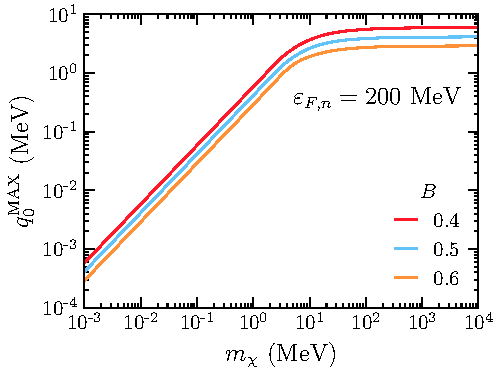
\includegraphics[width = 0.495\textwidth]{capture_1/q0max_mdm.pdf}
    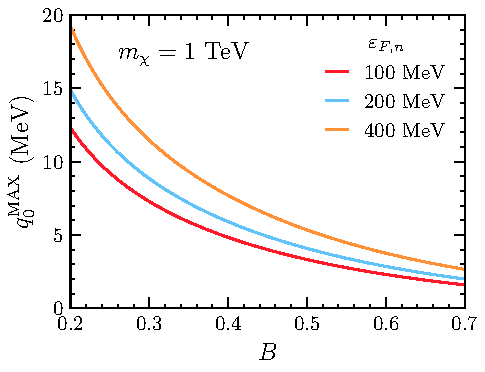
\includegraphics[width = 0.495\textwidth]{capture_1/q0max_B.pdf}

    \caption{Left: $\qomax$ vs. $m_\chi$ for $\kinFn=200\MeV$ and different values of B. 
    Right: $\qomax$ as a function of $B$ for different values of $\kinFi$ and $m_\chi=1\TeV$.}
    \label{ch3:fig:q0max}
\end{figure}
%%%%%%%%%%%%%%%%%%%%%%%%%%%%%%%%%%%%%%

%%%%%%%%%%%%%%%%%%%%%%%%%%%%%%%%%%%%%%
\begin{figure}[t!bp]
    \centering
    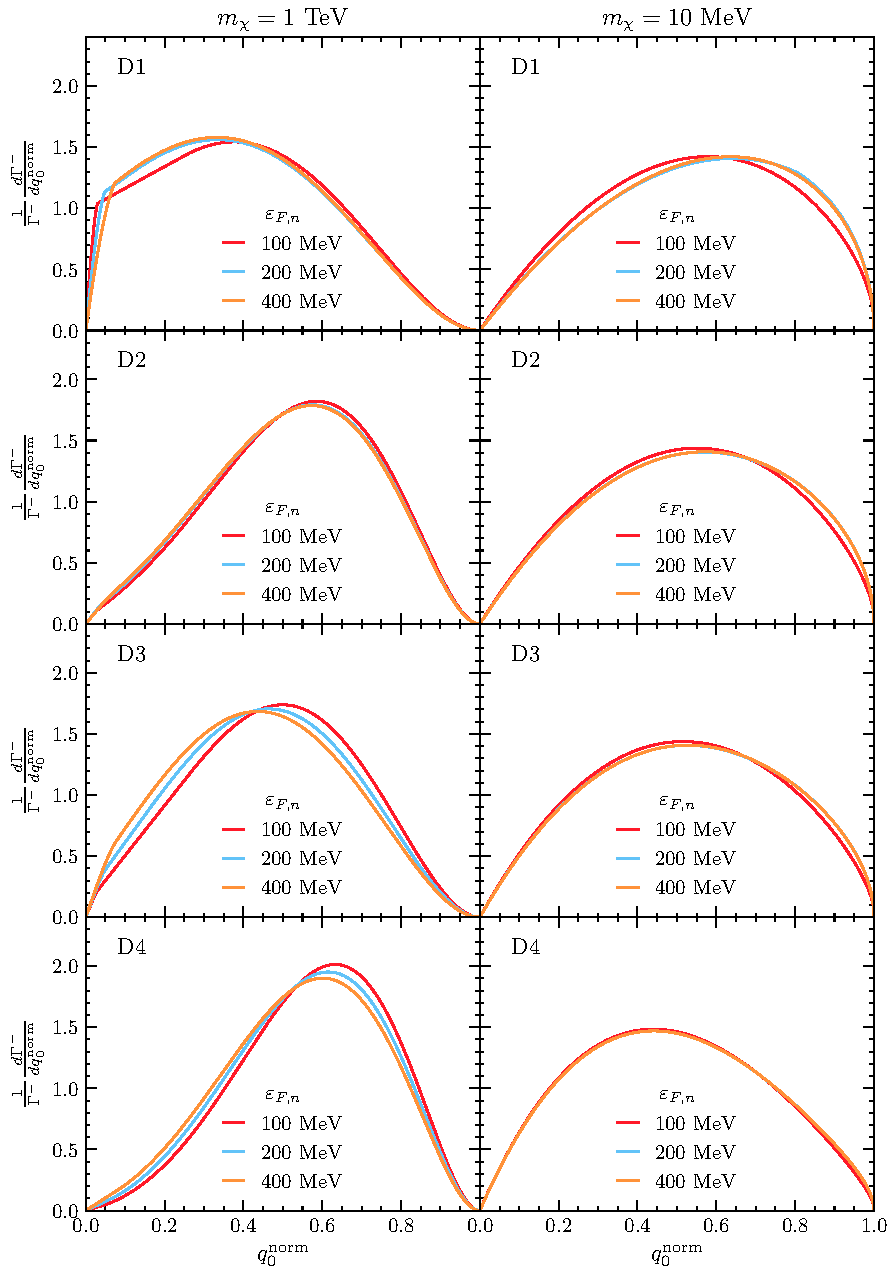
\includegraphics[width = 0.87\textwidth]{capture_1/norm_diff_intrate.pdf}    
    \caption[Normalised differential interaction rates $\frac{1}{\Gamma}\frac{d\Gamma}{d\qonorm}$ as a function of $\qonorm$.]{Normalised differential interaction rates $\frac{1}{\Gamma}\frac{d\Gamma}{d\qonorm}$ as a function of $\qonorm$ for different values of $\kinFn$, $m_\chi=1\TeV$ (left) and $m_\chi=10\MeV$ (right), $B=0.5$ and  operators D1 (first row), D2 (second row), D3 (third row) and D4 (fourth row). Profiles do not depend on $m_\chi$ in the limits $m_\chi\gg m_n$ (left) and $m_\chi\ll m_n$ (right).  }
    \label{ch3:fig:diffintratesd14}
\end{figure}
%%%%%%%%%%%%%%%%%%%%%%%%%%%%%%%%%%%%%%


Kinematics, and the phase space allowed by $h_j(x)$ in Eq.~\ref{ch3:eq:gamma_full_text}, determine the maximum energy that a DM particle can lose in a single scattering interaction, $\qomax$. The details of how to obtain $\qomax$ are given in Appendix~\ref{app:subsec:down_scatter_derivation}.
For DM capture, the value of $\qomax$ depends primarily on the DM mass, as is illustrated in the left panel of Fig.~\ref{ch3:fig:q0max}. We can see that for low $m_\chi$, $\qomax\propto m_\chi$, while, for $m_\chi\gg m_n$, it plataues to values between $\qomax\sim 3 - 6 \GeV$. 
%
Both $\qomax$ and $\frac{d\Gamma}{dq_0}$ also depend on $\kinFn$ and $B$. Changing $\kinFn$ has a very mild effect on the value of $\qomax$ (see right panel of Fig.~\ref{ch3:fig:q0max}) and on the shape of the normalised spectrum (see Fig.~\ref{ch3:fig:diffintratesd14}). On the other hand, increasing $B$ has the main effect of reducing   $\qomax$ (see right panel of Fig.~\ref{ch3:fig:q0max}), but only a mild effect on the shape of the profile expressed as a function of the normalised energy loss 
\begin{equation}
    \qonorm = \frac{q_0}{\qomax}. 
\end{equation}

We apply our results for $\frac{d\Gamma}{d q_0}$ to DM-neutron interactions, and in particular those with differential cross-sections that depend only on the transferred momentum $t=(k^\mu-k^{'\mu})^2$ and not on the centre of mass energy $s=(p^\mu+k^\mu)^2$.

In Fig.~\ref{ch3:fig:diffintratesd14} we show the normalised differential rates as a function of $\qonorm$ for the four operators D1-D4. The left-hand panels are in the limit $m_\chi\gg m_n$. We can observe that D1 has a softer spectrum, while the D2 and D4 spectra peak towards higher values of $q_0$. Varying the chemical potential $\kinFn$ has a very mild effect, shifting the spectrum to lower values of $q_0$ with increasing values of $\kinFn$.
Note that at small values of $\qonorm$ there is a sudden change in the slope of the normalised differential rate, which occurs for all operators but is more evident in D1 (top left panel). This is due to the zero temperature approximation, implicit in Eq.~\ref{ch3:eq:gamma_full_text}, where Heaviside functions were used to approximate FD distributions (see Appendix~\ref{app:subsec:down_scatter_derivation}); using a finite temperature would produce a smoother spectrum at small $\qonorm$. 

In the right-hand panels of Fig.~\ref{ch3:fig:diffintratesd14}, we explore the low DM mass region $m_\chi\ll m_n$. 
In this case, all operators give rise to similar profiles, the sole difference being that the peak of the profile is now shifted to lower  $\qonorm$ for D4 in contrast to D1, with intermediate values for D2 and D3. This is a consequence of Pauli blocking, with this effect depending on the specific power of $t$ that dominates the spectrum. Profiles with lower $n$ ($d\sigma\propto t^n$) peak at higher $\qonorm$ (see Fig.~\ref{ch3:fig:diffintratesd14}, right panels). For D4 we have $\Msq\propto t^2$, while the matrix elements of D2 and D3 are linear combinations of $t$ and $t^2$, and D1 is a combination of all powers of $t$. Comparing the right panels of Fig.~\ref{ch3:fig:diffintratesd14} with Fig.~\ref{app:fig:diffgamma}, we observe that the lowest power of $t$ determines the shape of the final differential interaction rate. Finally, varying $\kinFn$ has a very mild effect, this time shifting the spectrum mostly to higher values of $q_0$ for higher $\kinFn$.

The fact that the lowest power of $t$ dictates the features of the differential interaction rate is true also for the interactions that have a dependence on $s$. As such, by understanding the properties of the interaction rates with $\Msq\propto t^n$, we can understand the rates for all the operators in Table~\ref{ch1:tab:opers_defn_full}.


%%%%%%%%%%%%%%%%%%%%%%%%%%%%%%%%%%%%%%%%%
\subsection{Pauli Blocking}
\label{ch3:subsec:PB_cap}
%%%%%%%%%%%%%%%%%%%%%%%%%%%%%%%%%%%%%%%%%
% The DM interaction rate, Eq.~\ref{ch3:eq:scattrate}, is proportional to the number of target particles (nucleons/leptons) in the initial state with energy $\Ei$, and to the number of available final states with energy $\Ei+q_0$. 

The DM interaction rate, Eq.~\ref{ch3:eq:scattrate}, will be proportional to the number of target particles available to scatter off. Classically, this is the total number of targets within the star. However, the quantum degeneracy of the species within compact objects, due to the extreme densities, leads to a reduction in the number of available initial state target particles the DM can scatter off.
To understand this, consider the $T\rightarrow 0$ approximation, in which all initial states with energies $\Ei < \kinFi$ are occupied. These states are known as the ``Fermi sea". In order for the DM to scatter off one of these states, it must impart enough energy to kick the target out of the Fermi sea, such that 
\begin{equation}
    \Ei' = \Ei + q_0 > \kinFi,
\end{equation}
imposing a lower limit on the energy transfer required for an interaction to take place. This effectively reduces the number of available targets to only those with kinetic energies between $\kinFn - q_0$ and $\kinFi$. 
This suppression of the initial state phase space is known as Pauli blocking (PB), and is a completely quantum phenomenon.
In this limit, we necessarily have $\Gamma^-\rightarrow 0$ for $q_0\rightarrow 0$. 
It is also worth noting that Pauli blocking only affects the interaction rate when $q_0\le \kinFn$.


%%%%%%%%%%%%%%%%%%%%%%%%%%%%%%%%%%%%%%%%%
\begin{figure}[t!bp]
    \centering
    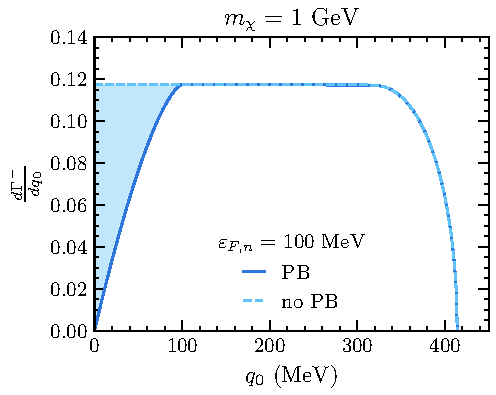
\includegraphics[width=.48\textwidth]{capture_1/diff_intrate_n0_mu_100MeV_mdm1GeV.pdf}
    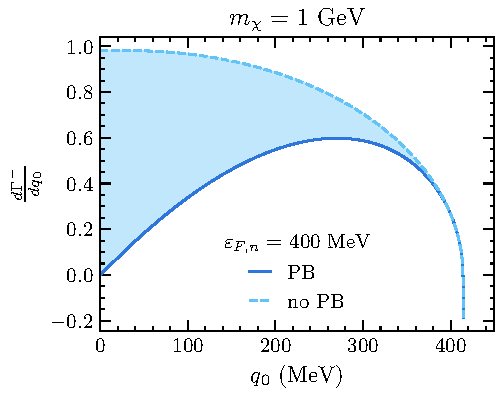
\includegraphics[width=.48\textwidth]{capture_1/diff_intrate_n0_mu_400MeV_mdm1GeV.pdf}\\
    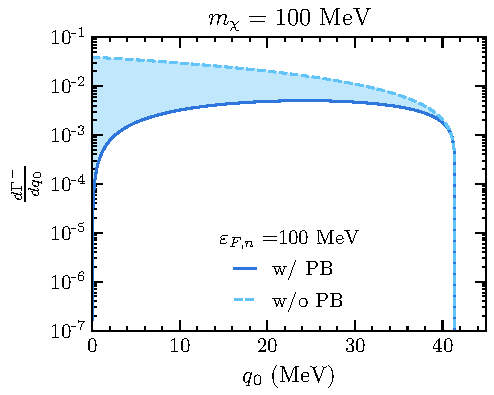
\includegraphics[width=.48\textwidth]{capture_1/diff_intrate_n0_mu_100MeV_mdm100MeV.pdf}
    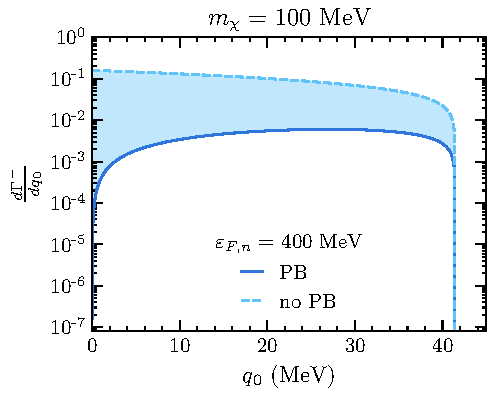
\includegraphics[width=.48\textwidth]{capture_1/diff_intrate_n0_mu_400MeV_mdm100MeV.pdf}\\
    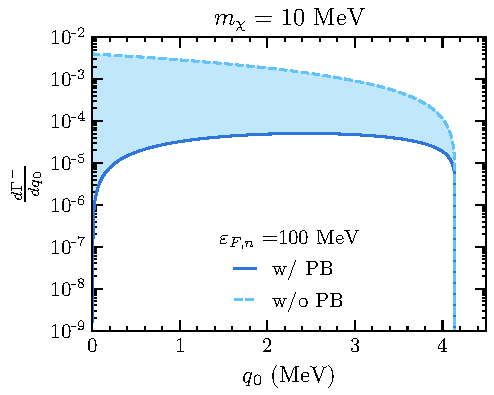
\includegraphics[width=.48\textwidth]{capture_1/diff_intrate_n0_mu_100MeV_mdm10MeV.pdf}
    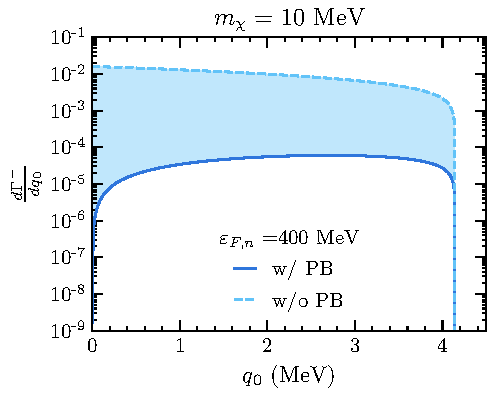
\includegraphics[width=.48\textwidth]{capture_1/diff_intrate_n0_mu_400MeV_mdm10MeV.pdf}
    \caption[Differential interaction rates $\frac{d\Gamma}{dq_0}$  
    as a function of the energy loss $q_0$ for different values of $m_\chi$ and $\kinFn$, constant cross-section and $B=0.5$.]{Differential interaction rates $\frac{d\Gamma}{dq_0}$  
    as a function of the energy loss $q_0$ for different values of $m_\chi$ and $\kinFn$, constant cross-section and $B=0.5$. Blue lines refer to the result that includes Pauli blocking, while the light blue dashed lines refer to the result without PB. Left column:  $\kinFn=100\MeV$, right column: $\kinFn=400\MeV$. Top: $m_\chi=1\GeV$, middle: $m_\chi=100\MeV$, bottom: $m_\chi=10\MeV$.}
    \label{ch3:fig:gammaNPBmu}
\end{figure}
%%%%%%%%%%%%%%%%%%%%%%%%%%%%%%%%%%%%%%%%%




To assess the impact of PB on the DM differential interaction rate, in Fig.~\ref{ch3:fig:gammaNPBmu} we compare the rate 
with (blue solid lines) and without (light blue dashed lines) Pauli blocking, for $B=0.5$ and constant DM-neutron cross-section. When Pauli blocking can be neglected, the interaction rate is obtained straightforwardly from Eq.~\ref{ch3:eq:scattrate} by stripping away the $(1 - \fFD(\Ei'))$ factor. 
The difference between the computations is shaded in light blue. In the top left panel, we see that the rate begins to be suppressed from PB at $q_0 \sim \kinFi = 100\MeV$ for a 1~GeV DM.
% we can see how the differential rate changes by switching Pauli blocking on or off, for $\kinFn=100\MeV$.
%  The rate calculated without PB is flat for $q_0\lesssim 200\MeV$, while when Pauli suppression is active it undergoes a smooth transition towards $0$ for $q_0<\kinFn$. 
In the top right plot, we increase the neutron chemical potential from $\kinFn=100\MeV$ to $\kinFn=400\MeV$. Given that in this case $\qomax \sim 0.4 m_\chi \sim 400\MeV$, almost the whole energy range is affected by PB. The higher $\kinFn$ changes the spectra (both with and without PB) such that the unsuppressed rate is no longer flat at low $q_0$. The PB suppressed rate reaches a maximum at values of $q_0$ slightly below $\qomax$, and then decreases towards $0$ at lower $q_0$.
In the middle panels, $m_\chi=100\MeV$, and $\qomax\sim40\MeV\ll\kinFn$. In this case, it is evident that PB affects the spectrum over the full $q_0=\qomax$ range. In the bottom row, we set $m_\chi=10\MeV$. As expected, for lighter DM,  the effects of PB are even more pronounced.



To understand how the effect of PB varies throughout the star, we can analyse the radial profiles of the capture rates $dC/dr$.
In Fig.~\ref{ch3:fig:diffcap} we plot the differential capture rate as a function of the NS radius, with and without Pauli blocking. We see that Pauli blocking is most significant at low DM mass, below about 1~GeV, and becomes insignificant for higher masses. Pauli blocking has a larger impact on the differential capture rate deeper into the NS interior and has a negligible effect at the surface. This is particularly apparent in the top left panel of Fig.~\ref{ch3:fig:diffcap}. This is because the chemical potential is higher in the NS interior than it is near the crust, as seen in the radial $\kinFi$ profile in the bottom left panel of Fig.~\ref{ch2:fig:BSk_profiles}.

%%%%%%%%%%%%%%%%%%%%%%%%%%%%%%%%%%%%%%%%%
\begin{figure}
    \centering
    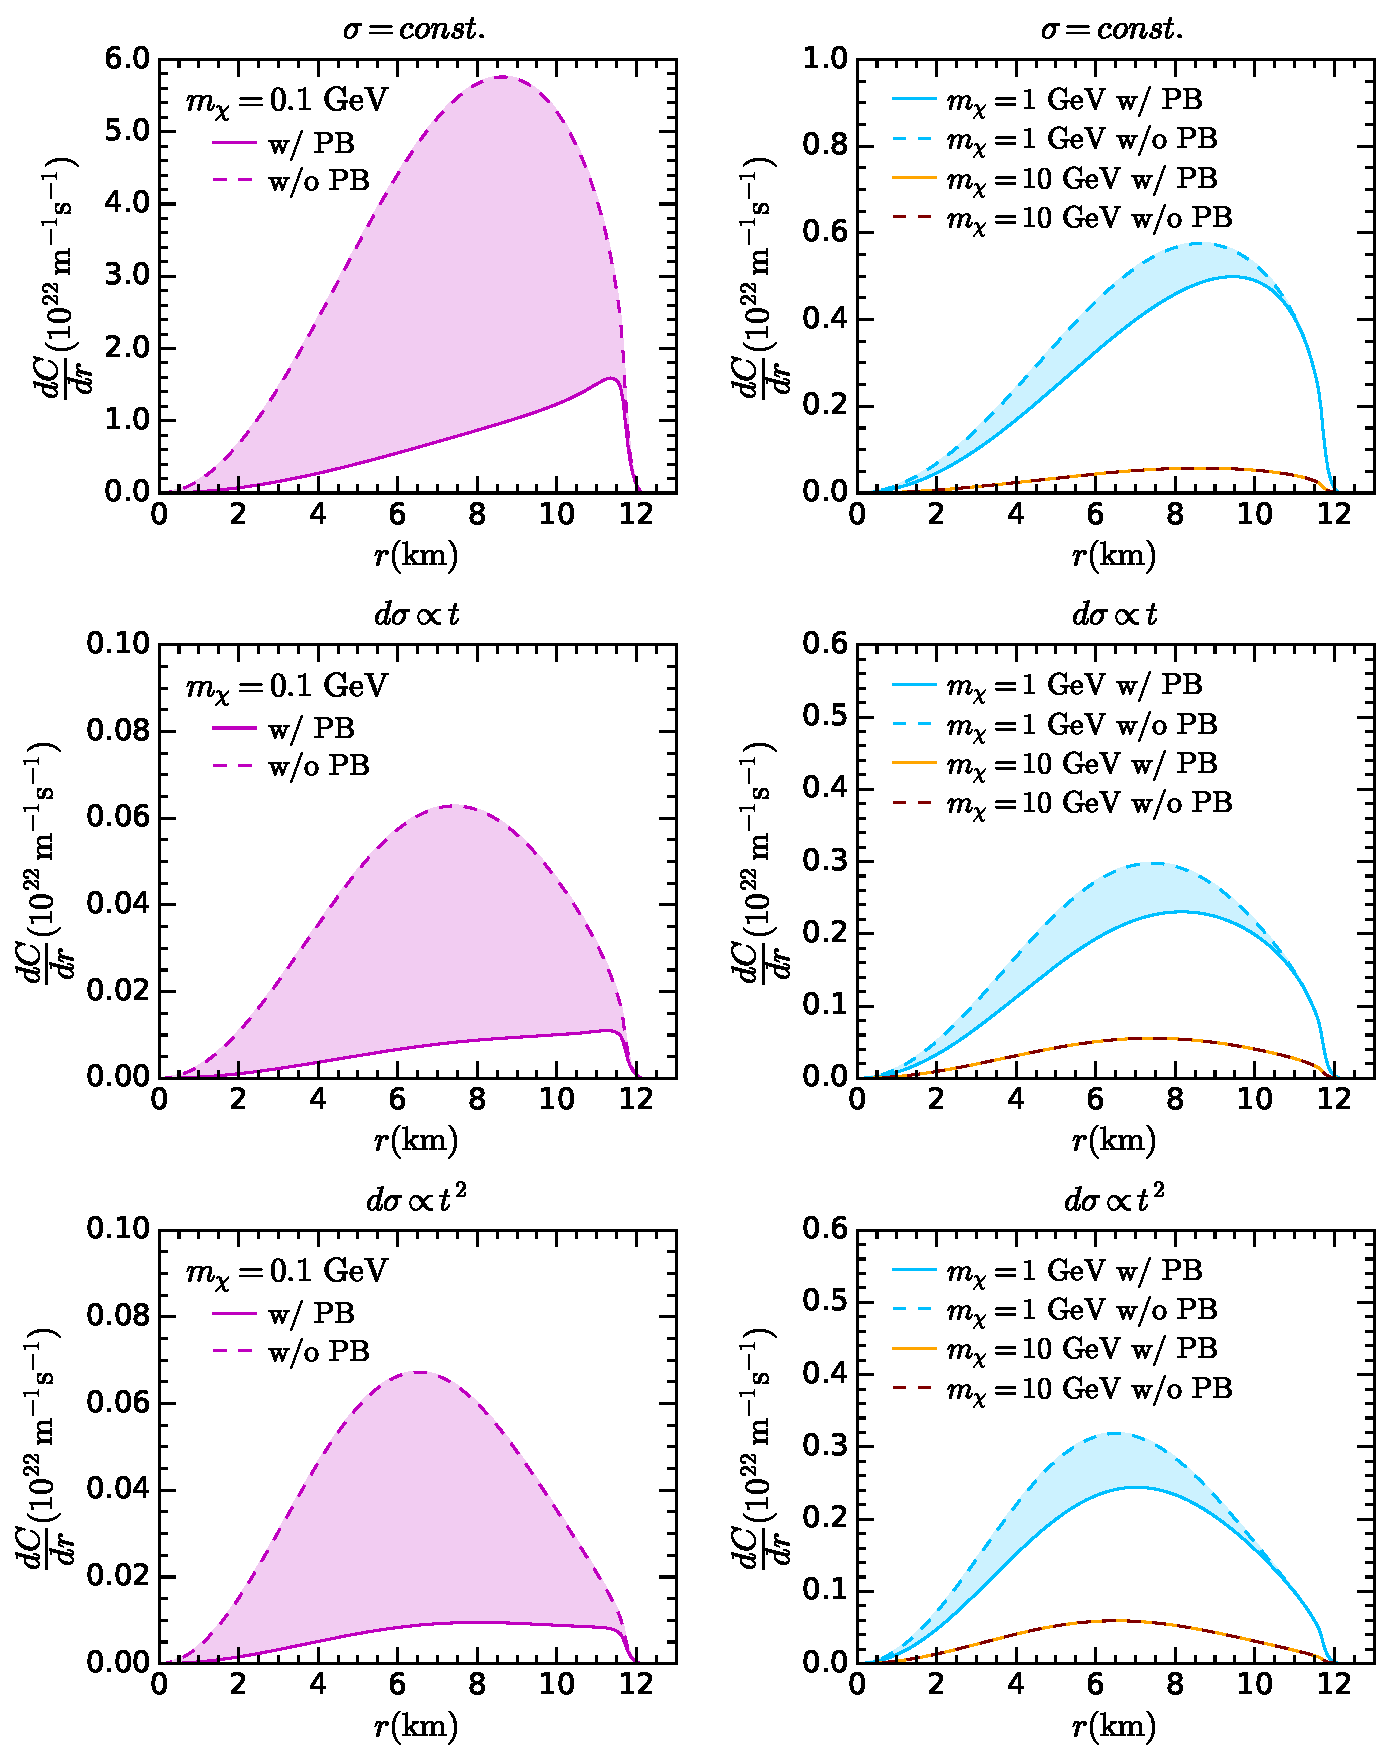
\includegraphics[width=.85\textwidth]{capture_1/diff_cap_rate.pdf}        
    \caption{Differential capture rate as a function of the NS radius $r$, with (solid) and without (dashed) Pauli blocking, for the EoS benchmark BSk24-2. Top: constant cross-section, center: $d\sigma\propto t$, bottom: $d\sigma\propto t^2$.}
    \label{ch3:fig:diffcap}
\end{figure}
%%%%%%%%%%%%%%%%%%%%%%%%%%%%%%%%%%%%%%%%%

%%%%%%%%%%%%%%%%%%%%%%%%%%%%%%%%%%%%%%%%%
%%%%%%%%%%%%%%%%%%%%%%%%%%%%%%%%%%%%%%%%%
%%%%%%%%%%%%%%%%%%%%%%%%%%%%%%%%%%%%%%%%%
\section{Capture in the Low, Intermediate and High Mass Regimes}
\label{ch3:sec:capture_analysis}
%%%%%%%%%%%%%%%%%%%%%%%%%%%%%%%%%%%%%%%%%
%%%%%%%%%%%%%%%%%%%%%%%%%%%%%%%%%%%%%%%%%
%%%%%%%%%%%%%%%%%%%%%%%%%%%%%%%%%%%%%%%%%

Having assembled all the required machinery, we are ready to explore the properties of the capture rate in the three mass regimes outlined in Eq.~\ref{ch3:eq:sigmath}.  Given the computational load required to evaluate Eq.~\ref{ch3:eq:cap_rel_full_1} in general, we aim to provide approximations that are numerically more efficient where possible. We also discuss the high DM mass regime where multiple scatterings are required for capture, and how this is affected by Pauli blocking. 


%%%%%%%%%%%%%%%%%%%%%%%%%%%%%%%%%%%%%%%%%
%%%%%%%%%%%%%%%%%%%%%%%%%%%%%%%%%%%%%%%%%
\subsection{Low and intermediate DM mass range}
\label{ch3:subsec:captureintermediate}
%%%%%%%%%%%%%%%%%%%%%%%%%%%%%%%%%%%%%%%%%
%%%%%%%%%%%%%%%%%%%%%%%%%%%%%%%%%%%%%%%%%


In sections~\ref{ch3:sec:captrue_new_full} and \ref{ch3:sec:diff_int_rate}, we have derived general expressions to numerically calculate the DM capture and interaction rates,  
Eqs.~\ref{ch3:eq:cap_rel_full_1} and \ref{ch3:eq:int_rate_capture_full} respectively.   
Using these expressions, we can write 
the complete expression for the capture rate as a function of the differential DM-neutron cross-section 
\begin{equation}
    \begin{split}
        C = \frac{2\rho_\chi}{\pi \vstar m_\chi^2} {\rm Erf}\left(\sqrt{\frac{3}{2}}\frac{\vstar}{v_d}\right)\int_0^{\Rstar}  dr  \frac{r^2\zeta(r)}{\sqrt{B(r)}} &\int dt d\Ei ds \frac{d\sigma}{d\cos\thetacm}\frac{\Ei s}{\beta(s)\gamma(s)}\\
        &\times \fFD(\Ei,r)(1-\fFD(\Ei',r)), 
    \end{split}
\label{ch3:eq:capturefinal}
\end{equation}
where the functions $\beta$ and $\gamma$ were given in Section~\ref{ch3:subsec:int_rate_degen_rel}. Recall that in the limit $T\rightarrow0$,  $\fFD(\Ei,r)$ and $1-\fFD(\Ei',r)$  reduce to the step functions,  $\Theta(\kinFi(r)-\Ei)$ and  $\Theta(\Ei'-\kinFi(r))$, respectively. 


Exchanging the differential cross-section for the squared matrix allows for easier examination of the operators in Table~\ref{ch1:tab:opers_defn_full}, and so we write the capture rate as
\begin{equation}
    \begin{split}
        C &=  \frac{\rho_\chi}{8\pi^2 \vstar m_\chi^2} {\rm Erf}\left(\sqrt{\frac{3}{2}}\frac{\vstar}{v_d}\right)\int_0^{\Rstar}   dr  \frac{r^2 \zeta(r) }{\sqrt{B(r)}} & \int dt d\Ei ds \frac{\Msq \Ei}{2s\beta(s)-\gamma^2(s)} \frac{s}{\gamma(s)} \\
        &\times \fFD(\Ei,r)(1-\fFD(\Ei',r)). 
    \end{split}
    \label{ch3:eq:capturefinalM2}
\end{equation}
This expression can be used to numerically calculate the single scatter capture rate of DM in compact objects, in the optically thin regime. In general, this must be used for low-mass DM where PB is in effect.

As discussed in Section~\ref{ch3:subsec:PB_cap}, PB eventually becomes negligible for DM with masses $\gtrsim \muFi$. Hence, between this mass and the point where multiple scattering becomes important, PB can be neglected and a simplified capture rate be obtained. For nucleon targets, this range is between $1\GeV\lesssim m_\chi\lesssim 10^6\GeV$, which we call the intermediate mass range.

The resulting simplified capture rate differs slightly depending on whether the matrix element depends only on $t$, or if it has explicit $s$ dependence. We present the full derivations of these results in Appendix~\refeq{app:sec:capratesimple}
First, for $\Msq=a t^n$, the previous expression can be simplified to 
\begin{gather}
        C \sim C_\mathrm{approx} = \frac{4\pi}{\vstar} \frac{\rho_\chi}{m_\chi}{\rm Erf}\left(\sqrt{\frac{3}{2}}\frac{\vstar}{v_d}\right)\int_0^{\Rstar}  r^2 dr \, n_i(r)  \frac{1-B(r)}{B(r)} \langle\sigma(r)\rangle 
\label{ch3:eq:csimplelargemtext}, \\
\langle\sigma(r)\rangle = \left\langle\int dt \frac{d\sigma}{dt} \right\rangle_s =   \frac{a}{16\pi m_\chi^2 } \frac{1}{n+1}\left(\frac{4(1-B(r))m_\chi^2}{B(r)(1+\mu^2)}\right)^{n}. 
\label{ch3:eq:xsecave}
\end{gather}
For $s$-dependent matrix elements the result is very similar, with the only difference being that the cross-section is not averaged over $s$, and instead $s$ is fixed to a particular value as detailed in Appendix~\refeq{app:sec:capratesimple}. Writing the matrix element as $\Msq \propto \bar{g}(s)t^n$, for with $g$ some function of $s$, we arrive at the result
\begin{gather}
    C \sim C_{\mathrm{approx}, s} = \frac{4\pi}{\vstar} \frac{\rho_\chi}{m_\chi}{\rm Erf}\left(\sqrt{\frac{3}{2}}\frac{\vstar}{v_d}\right)\int_0^{\Rstar}  r^2 dr \, n_i(r)  \frac{1-B(r)}{B(r)} \sigma(r)
\label{ch3:eq:csimplelargemtext_sdep}, \\
\begin{split}
    \sigma(r) = \int dt \frac{d\sigma}{dt} & =   \frac{1}{16\pi \left(\mi^2 \mchi^2 + 2\mi \mchi/\sqrt{B(r)}\right)}\frac{\bar{g}(s_0)}{(n+1)}\\
    &\hspace{6em}\times\left[\frac{4(1 - B(r)) \mchi^2}{B(r)(1 + \mu^2) + 2\sqrt{B(r)}\mu}\right]^n,
\label{ch3:eq:xsecave_sdep}
\end{split}\\
s_0 = \mi^2 + \mchi^2 + 2\frac{\Ei\mchi}{\sqrt{B(r)}}.\label{ch3:eq:s0}
\end{gather}
As with the differential interaction rates, it is the $t$-dependence of the matrix elements that dictate the key features of the capture rate.

%%%%%%%%%%%%%%%%%%%%%%%%%%%%%%%%%%%%%%%
\begin{figure}
    \centering
    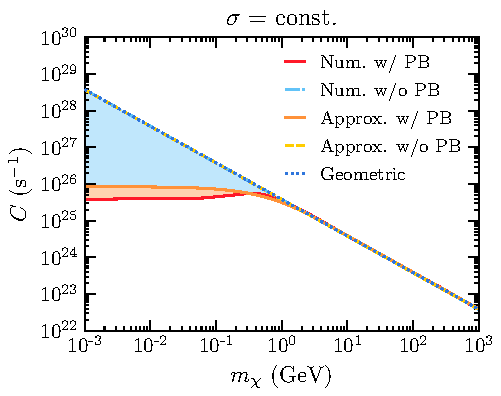
\includegraphics[width=.48\textwidth]{capture_1/capture_rate_n0.pdf}
    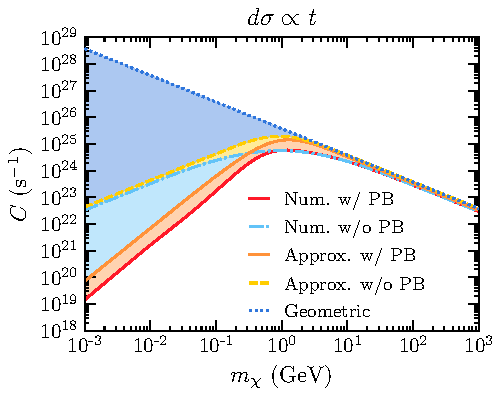
\includegraphics[width=.48\textwidth]{capture_1/capture_rate_n1.pdf}\\
    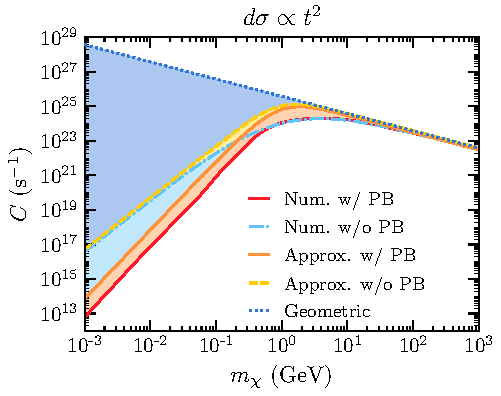
\includegraphics[width=.48\textwidth]{capture_1/capture_rate_n2.pdf}
    \caption[Capture rate as a function of the DM mass with cross-sections normalised to $\sigma=\sigmaref\sim 1.7 \times 10^{-45} \cm^2$, for EoS BSk24-2, calculated with and without Pauli blocking.]{Capture rate as a function of the DM mass with cross-sections normalised to $\sigma=\sigmaref\sim 1.7 \times 10^{-45} \cm^2$, for EoS BSk24-2, calculated with and without Pauli blocking. Top left: constant cross-section. Top right: $d\sigma\propto t$, bottom: $d\sigma\propto t^2$, where $t$ is the Mandelstam variable. All rates are normalised to the geometric limit at large DM mass. }
    \label{ch3:fig:approxc}
\end{figure}
%%%%%%%%%%%%%%%%%%%%%%%%%%%%%%%%%%%%%%%


In Fig.~\ref{ch3:fig:approxc}, we show the capture rate as a function of the DM mass for matrix elements proportional to $t^n$, for $n=0,1,2$ and the NS benchmark model BSk24-2. Numerical results obtained using Eq.~\ref{ch3:eq:capturefinalM2} are shown in solid red; results using the same equation but removing the theta function that enforces Pauli blocking are depicted in light blue; and the approximation for intermediate DM masses, Eq.~\ref{ch3:eq:csimplelargemtext}, in yellow. We show the geometric limit, Eq.~\ref{ch3:eq:capturegeom}, in blue for comparison. 
The capture rates were all normalised to the geometric limit at large DM mass where PB is negligible. 
In the same plots, we also show in brown the result obtained from using a modified version of Eq.~\ref{ch3:eq:csimplelargemtext} to include Pauli blocking.
This is achieved by including the ratio between the differential the interaction rate, $\Gamma^-$, calculated with and without Pauli blocking. This comparison was done in Section~\ref{ch3:subsec:PB_cap} for various values of $B$ and $\kinFn$.

From Fig.~\ref{ch3:fig:approxc}, we can see that Eq.~\ref{ch3:eq:csimplelargemtext} is indeed a good approximation to the numerical results obtained without Pauli blocking, and can be safely used for DM masses from a few $\GeV$ up to $m_\chi\sim10^6\GeV$, where multiple scattering becomes relevant. 
On the other hand, for $m_\chi\lesssim 100\MeV$ the brown line is no longer a good approximation to the numerical result with Pauli blocking, as it always overestimates the capture rate by nearly an order of magnitude. Therefore, to accurately account for the effects of PB for low mass DM, the complete expression for the capture rate, Eq.~\ref{ch3:eq:capturefinalM2} must be used and evaluated numerically.

We now compare our full numerical capture rate calculation, Eq.~\ref{ch3:eq:capturefinalM2}, with that of Ref.~\cite{Garani:2018kkd_may_NewAnalysisNeutron}, in Fig.~\ref{ch3:fig:Cratecomp}. The capture rates calculated in Ref.~\cite{Garani:2018kkd_may_NewAnalysisNeutron} correctly include the stellar structure and Pauli blocking, however, they do not account for general relativistic corrections, and the authors only considered the case of a constant cross-section, $\sigma=10^{-45}\cm^2$. Top make the comparison as fair as possible, we have selected NS configurations that match those of Figs.~1 and 14 of Ref.~\cite{Garani:2018kkd_may_NewAnalysisNeutron}, namely their Model A (BSk20-1):  $\Mstar\simeq1.52\Msun$, $\Rstar\simeq11.6\km$ and Model D (BSk21-2): $\Mstar\simeq2.11\Msun$ and $\Rstar\simeq12.0\km$. We denote these new benchmark models as BSk26-1 (left panel of Fig.~\ref{ch3:fig:Cratecomp}) and BSk24-5 (right panel). Note that we were not able to use the BSk20 and BSk21 functionals, since there are no publicly available fits for the chemical potentials and particle abundances for those EoS families. However, as discussed earlier in section \ref{ch2:subsec:NS_EoS}, BSk26 (BSk24) yields configurations that are almost indistinguishable from those obtained with BSk20 (BSk21)~\cite{Perot:2019gwl_Rolesymmetryenergy}.

We can see in the left panel of Fig.~\ref{ch3:fig:Cratecomp} that in the non-Pauli suppressed region, $m_\chi \gtrsim 1\GeV$, our capture rate calculation in the optical thin limit (solid magenta) exceeds that of Ref.~\cite{Garani:2018kkd_may_NewAnalysisNeutron} (dot-dashed blue) by a factor of $\sim 4$. When Pauli blocking is active, our capture rate calculation is about one order of magnitude higher than the classical calculation.  Recall that Ref.~\cite{Garani:2018kkd_may_NewAnalysisNeutron}  accounts for neither gravitational focusing nor relativistic kinematics. 
We also show in dashed light blue the approximation given in Ref.~\cite{McDermott:2010pa_TurningLightsHow}, which accounts for Pauli blocking with a suppression factor that depends on the neutron Fermi momentum $\sim m_\chi v_{esc}/p_{F,n}$ for $m_\chi < m_n$. Though this approximation fails to reproduce the capture rate shape due to Pauli blocking in the DM mass range $[0.1\GeV,10\GeV]$, it underestimates the capture rate by only a factor of 2 when the DM mass is below 0.1 GeV. 
Finally, we compare the geometric limit of Eq.~\ref{ch3:eq:capturegeom}  (solid orange) that incorporates GR effects~\cite{Bell:2018pkk_sep_HeatingNeutronStars} with the non-relativistic expression in Ref.~\cite{Garani:2018kkd_may_NewAnalysisNeutron} (dot-dashed brown). We observe that the former is $\sim 67 \%$ greater than the latter, mostly due to the $1/B(\Rstar)$ GR correction \cite{Goldman:1989nd_WeaklyInteractingMassive,Kouvaris:2007ay_WIMPAnnihilationCooling}. Similar conclusions are obtained when comparing capture rate calculations for Model D of Ref.~\cite{Garani:2018kkd_may_NewAnalysisNeutron} (their Fig.~14) with our approach, as illustrated in the right panel of Fig.~\ref{ch3:fig:Cratecomp}.

%%%%%%%%%%%%%%%%%%%%%%%%%%%%%%%%%%%%%%%%
\begin{figure}
    \centering
    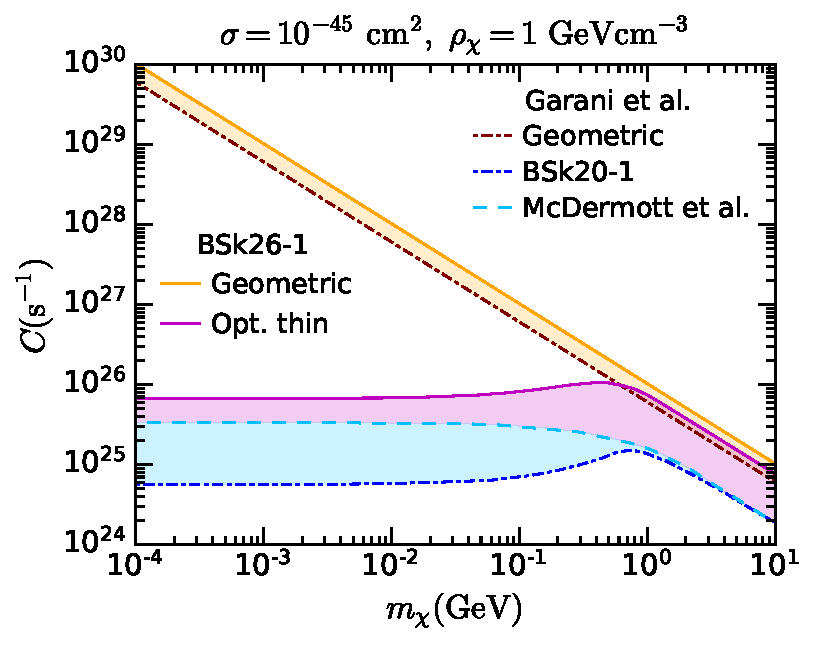
\includegraphics[width=.48\textwidth]{capture_1/capture_rate_n0_comp1.pdf}
    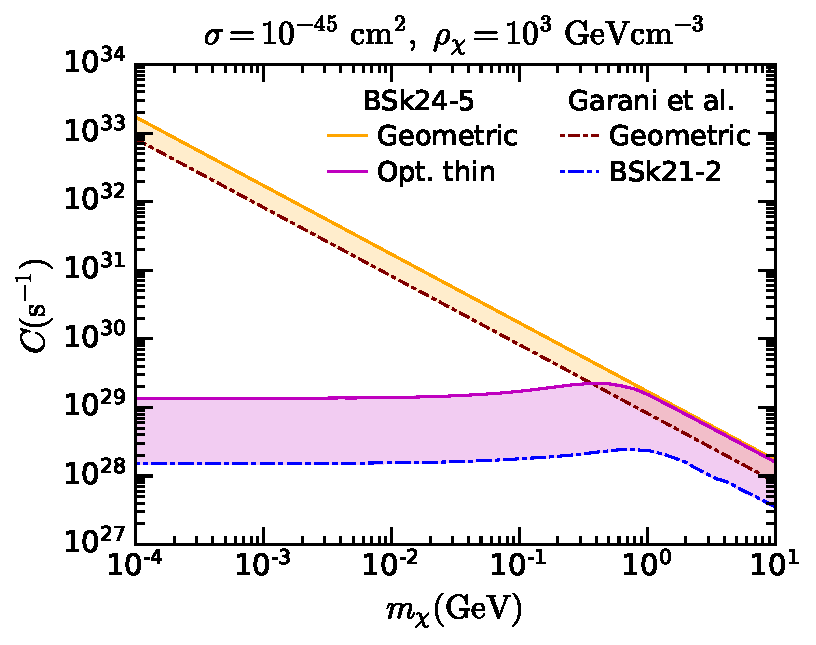
\includegraphics[width=.48\textwidth]{capture_1/capture_rate_n0_comp2.pdf}    
    \caption[Capture rate in the optically thin  (magenta) and geometric (orange) limits as a function of the DM mass for constant cross-section $\sigma=10^{-45}\cm^2$, $\rho_\chi=1\GeV\cm^{-3}$ and BSk26 functional for $\Mstar\simeq1.52\Msun$ and $\Rstar\simeq11.6\km$ denoted as BSk26-1.]{Left: Capture rate in the optically thin  (magenta) and geometric (orange) limits as a function of the DM mass for constant cross-section $\sigma=10^{-45}\cm^2$, $\rho_\chi=1\GeV\cm^{-3}$ and BSk26 functional for $\Mstar\simeq1.52\Msun$ and $\Rstar\simeq11.6\km$ denoted as BSk26-1. Capture rate calculations from Ref.~\cite{Garani:2018kkd_may_NewAnalysisNeutron} for a NS configuration with EoS BSk20-1~\cite{Potekhin:2013qqa_Analyticalrepresentationsunified} equivalent to BSk26-1, are shown for comparison. Right: Same as left but for $\rho_\chi=10^3\GeV\cm^{-3}$ and the benchmark model BSk24-5 equivalent to BSk21-2 in Ref.~\cite{Garani:2018kkd_may_NewAnalysisNeutron}: $\Mstar\simeq2.11\Msun$ and $\Rstar\simeq12.0\km$. 
    }
    \label{ch3:fig:Cratecomp}
\end{figure}
%%%%%%%%%%%%%%%%%%%%%%%%%%%%%%%%%%%%%%%%

%%%%%%%%%%%%%%%%%%%%%%%%%%%%%%%%%%%%%%%%
%%%%%%%%%%%%%%%%%%%%%%%%%%%%%%%%%%%%%%%%
\subsection{Large Mass Regime: Multiple Scattering}
\label{ch3:subsec:largemassandsigma}
%%%%%%%%%%%%%%%%%%%%%%%%%%%%%%%%%%%%%%%%
%%%%%%%%%%%%%%%%%%%%%%%%%%%%%%%%%%%%%%%%


The capture rate expressions obtained in the previous section assume that the cross-section is small enough that the star is in the ``optically thin'' regime, and that a single scatter is sufficient to capture the DM. These assumptions break down if the DM-target cross-section is $\gtrsim\mathcal{O}(\sigmath)$, or if the DM mass exceeds $m_\chi \sim 10^6\GeV$, respectively. 
In this section, we focus on addressing the latter concern as we work in the optically thin regime for the remainder of this work\footnote{The discussion on the effect of the NS opacity in $\sigma\sim \sigmath$ regime can be found in Ref.~\cite{Bell:2020jou_sep_ImprovedTreatmentDark}.}. 
To that end, we now explain how to modify our previous capture rate expressions to account for multiple scattering in a degenerate media\footnote{For a recent discussion on multiple scattering within non-relativistic stars, or with ions in WDs, see Ref.~\cite{Dasgupta:2019juq_Darkmattercapture}.}


In deriving Eq.~\ref{ch3:eq:capturefinal} we had assumed that the DM velocity at infinity, $u_\chi$, can be neglected, such that any interaction where the DM loses energy resulted in its capture. If we instead keep the leading order $u_\chi$ contribution to the total DM energy, the DM energy at infinity is
\begin{equation}
    E^\infty_\chi \sim m_\chi \left(1+\frac{1}{2}u_\chi^2\right), 
\end{equation}
and at a distance $r$ from the star, it gets boosted to
\begin{equation}
    E_\chi(r) = \frac{m_\chi}{\sqrt{B(r)}} \left(1+\frac{1}{2}u_\chi^2\right).
    \label{ch3:eq:Echir}
\end{equation}
Therefore, the amount of energy that the DM must lose to be captured is
\begin{align}
    E_\chi^C(r) & =  \frac{1}{2}u_\chi^2 \frac{m_\chi}{\sqrt{B(r)}}. \\
                & \sim 0.6\GeV \left(\frac{u_\chi}{270\km\s^{-1}}\right)^2 \left(\frac{m_\chi}{10^6\GeV}\right)\left(\frac{0.5}{B(r)}\right)^{1/2}.
\end{align} 
Hence, DM with a mass of $10^6\GeV$ with an initial velocity $u_\chi = 270\km\s^{-1}$, must lose 0.6 GeV of energy for it to be captured. This is of the same order as the maximum amount of energy that can be lost in a single scatter as seen in Fig.~\ref{ch3:fig:q0max}. Given that $\qomax$ plates for $\mchi \gg \mi$, it will be highly improbable that DM heavier than $\sim 10^6\GeV$ loses enough energy in a single scatter to be captured. Single scatter capture is still possible as the DM velocity at infinity is not a fixed value, rather it follows by some distribution function. Therefore, the heavy DM could have a velocity close to zero at infinity, significantly reducing the amount of energy it needs to lose.

To account for this effect, we assume that the DM particles have a speed $u_\chi\ll 1$ at infinity that follows a Maxwell-Boltzmann (MB) distribution, Eq.~\ref{ch3:eq:MB}. 
We can then define the probability density function (PDF) of the energy lost by the DM using the differential interaction rate through
\begin{equation}
\xi(q_0,E_\chi,\kinFi) = \frac{1}{\Gamma^{-}(E_\chi)}\frac{d\Gamma^{-}}{dq_0}(q_0,E_\chi,\kinFi),\label{ch3:eq:normintrate}
\end{equation}
where $\frac{d\Gamma}{dq_0}$ is the DM differential interaction rate, calculated in Appendix~\ref{ch3:sec:diff_int_rate}. 
The function $\xi$ is defined for any $q_0\ge 0$, however, kinematics dicatates that the function is non-zero only for $q_0\le\qomax$. Additionally, note that $\xi$ depends on $B(r)$ through the ratio $E_\chi/m_\chi$, and for brevity we will simply write $\xi(q_0)$.



%%%%%%%%%%%%%%%%%%%%%%%%%%%%%%%%%%
\begin{figure}[t]
    \centering
    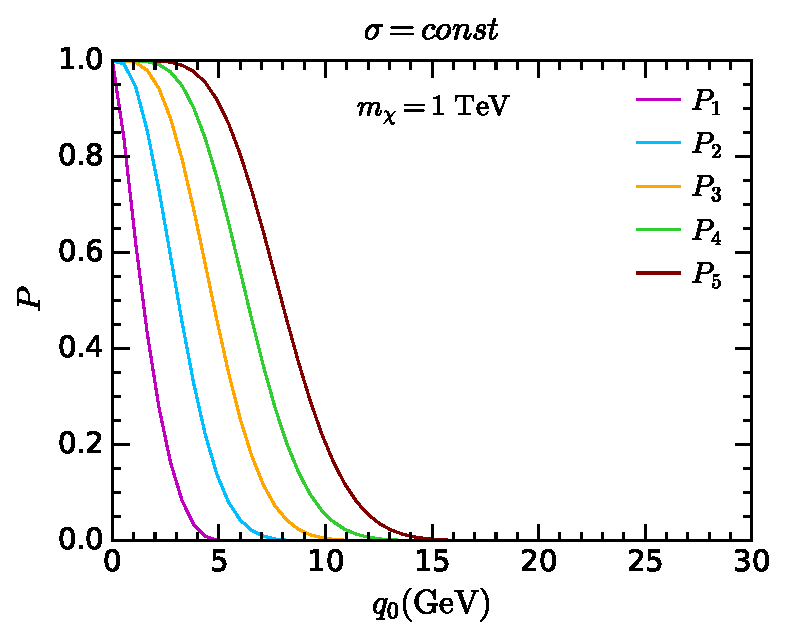
\includegraphics[width=.48\textwidth]{capture_1/probs_n0.pdf}
    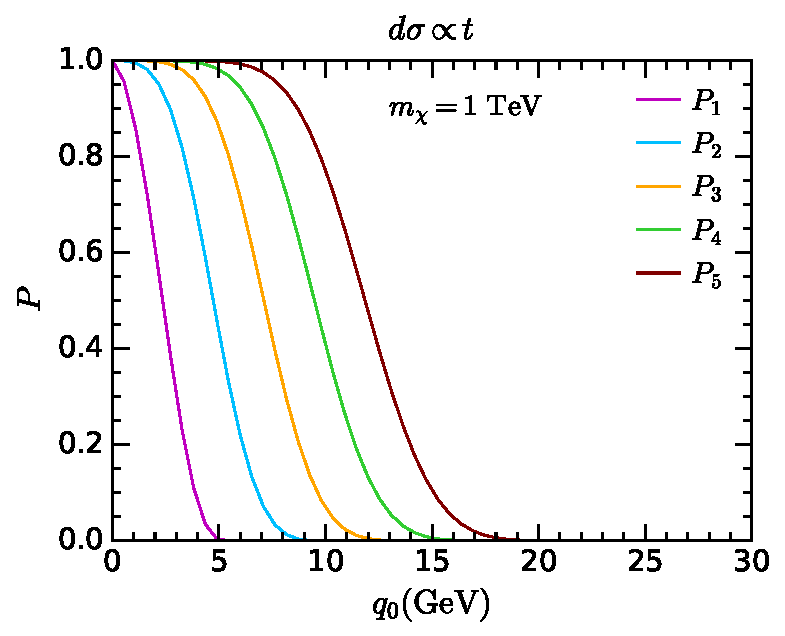
\includegraphics[width=.48\textwidth]{capture_1/probs_n1.pdf}\\
    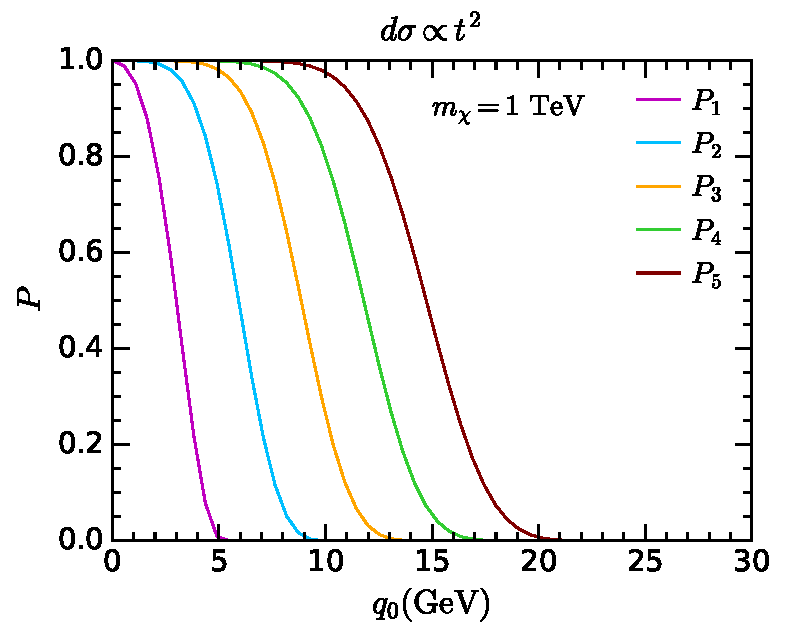
\includegraphics[width=.48\textwidth]{capture_1/probs_n2.pdf}
    \caption[Probabilities to lose at least an amount of energy $\delta q_0$  after $1,...,5$ scatterings,  $P_1,...,P_5$, as a function of the energy loss $q_0$,  assuming $B=0.5$ and $\kinFn=400\MeV$.]{Probabilities to lose at least an amount of energy $\delta q_0$  after $1,...,5$ scatterings,  $P_1,...,P_5$, as a function of the energy loss $q_0$,  assuming $B=0.5$ and $\kinFn=400\MeV$. Results are shown for different dependence on the cross-section on the Mandelstam variable $t$: constant DM-neutron cross-section (top left), $d\sigma\propto t$ (top right) and $d\sigma\propto t^2$ (bottom). }
    \label{ch3:fig:pn}
\end{figure}
%%%%%%%%%%%%%%%%%%%%%%%%%%%%%%%%%%%


We can define the probability of losing at least an amount of energy $q_0 = \delta q_0$ in a single collision as
\begin{equation}
    P_1(\delta q_0) = \int_{\delta q_0}^\infty dx \xi(x).
    \label{ch3:eq:P1}
\end{equation}
The probability of losing at least the same amount of energy after 2 collisions will then be
\begin{align}
 P_2(\delta q_0) &= \int_{\delta q_0}^\infty dy \int_0^\infty dx\;\xi(x) \xi(y-x)\\
    & =  P_1(\delta q_0) + \int_{\delta q_0}^\infty dy \int_0^y dx\; \xi(x)\xi(y-x)\\
    & = P_1(\delta q_0) + \int_0^{\delta q_0} dz \;P_1(\delta q_0-z)\xi(z).
\end{align}
From this, we obtain the following recursive relation for the probabilities, $P_N$, of losing at least $q_0 = \delta q_0$ in $N$ scatters,
\begin{equation}
 P_{N+1}(\delta q_0) = P_N(\delta q_0) + \int_0^{\delta q_0} dz P_N(\delta q_0-z)\xi(z).\label{ch3:eq:pnrecurrent}
\end{equation} 
In Fig.~\ref{ch3:fig:pn} we show how the probability functions $P_1,...,P_5$ changes based on the $t$ dependence of the differential cross-section. We show results for $\sigma=$const. (top left), $d\sigma\propto t$ (top right) and $d\sigma\propto t^2$ (bottom), for fixed values of $B=0.5$, $\kinFn=400\MeV$.

%%%%%%%%%%%%%%%%%%%%%%%%%%%%%%
\begin{figure}
    \centering
    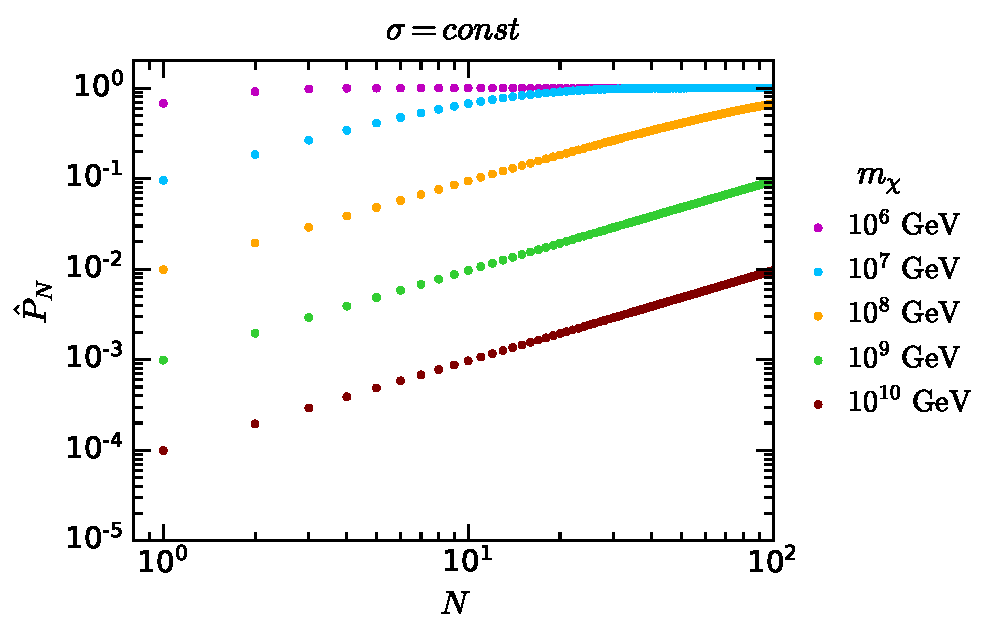
\includegraphics[width=.6\textwidth]{capture_1/cumprobN_n0.pdf}
    \caption[Cumulative probability $\hat{P}_N$ for $B=0.5$,  $\kinFn=400\MeV$ and for $\sigma = \mathrm{const.}$ as a function of the number of scatterings $N$ for several DM masses.]{Cumulative probability $\hat{P}_N$ for $B=0.5$,  $\kinFn=400\MeV$ and for $\sigma = \mathrm{const.}$ as a function of the number of scatterings $N$ for several DM masses.}
    \label{ch3:fig:pnofn}
\end{figure}
%%%%%%%%%%%%%%%%%%%%%%%%%%%%%%

To connect this back to the capture probability, we define the probability for a DM particle to be captured after exactly $N$ interactions, $c_N$, to be $P_N(E^C_\chi) - P_{N-1}(E^C_\chi)$ averaged over the MB distribution of the initial velocity,
\begin{equation}
    \begin{split}
        c_N(r) &= \frac{1}{\int_0^\infty \frac{\fMB(u_\chi)}{u_\chi}du_\chi}\int_0^\infty \frac{\fMB(u_\chi)}{u_\chi}du_\chi \left[P_N\left(\frac{1}{2}\frac{m_\chi u_\chi^2}{\sqrt{B(r)}}\right)\right.\\
        &\hspace{18em}\left. -P_{N-1}\left(\frac{1}{2}\frac{m_\chi u_\chi^2}{\sqrt{B(r)}}\right)\right], 
    \end{split}
\end{equation}
where $c_N$ depends on $r$ through the dependence of $P_N$  on $B(r)$ and $\kinFn(r)$. Note that although our results will assume a Maxwell-Boltzmann velocity distribution, it is straightforward to generalise the results to any other DM velocity distribution. The cumulative probability $\hat{P}_N$ that a DM particle is captured after $N$ interactions with a total energy loss  $\delta q_0=E_\chi^C$ is then
\begin{equation}
\hat{P}_N(r) = \sum_{i=1}^N c_i = \frac{1}{\int_0^\infty \frac{\fMB(u_\chi)}{u_\chi}du_\chi}\int_0^\infty \frac{\fMB(u_\chi)}{u_\chi}du_\chi P_N\left(\frac{1}{2}\frac{m_\chi}{\sqrt{B(r)}} u_\chi^2\right).
\end{equation}
%
The resulting cumulative probability is shown as a function of the number of scatterings $N$ in Fig.~\ref{ch3:fig:pnofn}, for constant cross-section and several DM masses. 

The cumulative probability $\hat{P}_N$ for the above values of $B,\kinFn$ is well approximated by the function\footnote{Further discussion of the multi-scattering regime, and justification of this fitting function, can be found in Appendix~C of Ref.~\cite{Bell:2020jou_sep_ImprovedTreatmentDark}.}
\begin{equation}
\hat{P}_N \sim  1-e^{-\frac{N \mstar}{m_\chi}}.\label{ch3:eq:pncum}
\end{equation}
In particular, the probability that the DM is captured in a single scatter is 
\begin{equation}
c_1=\hat{P}_1 \sim  1-e^{-\frac{\mstar}{m_\chi}}.
\label{ch3:eq:c1}
\end{equation}
From this, we see that $c_1$ will begin to significantly fall below unity for $\mchi \gtrsim \mstar$, and hence multiple scattering will only significantly reduce the capture rate for DM masses above $\mstar$. 

To give an idea for how large the value of $\mstar$ will be, for neutron targets and the values $B=0.5$ and $\kinFn=400$~MeV, we find
\begin{align}
m^{*} &=1.08 \times 10^6 \GeV,\quad \Msq\propto t^0,\\
m^{*} &=1.62 \times 10^6 \GeV,\quad \Msq\propto t^1,\\
m^{*} &=2.01 \times 10^6 \GeV,\quad \Msq\propto t^2.
\end{align}
We illustrate how $m^*_n$ varies with $B$ and $\kinFn$ in Fig.~\ref{ch3:fig:mstarbmu}. 

%%%%%%%%%%%%%%%%%%%%%%%%%%%%%%
\begin{figure}[t!bp]
    \centering
    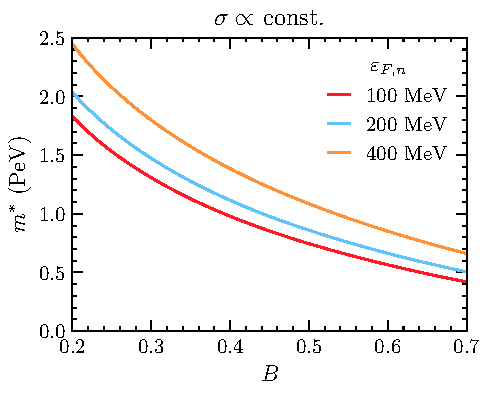
\includegraphics[width=.48\textwidth]{capture_1/mstar_B_n0.pdf}
    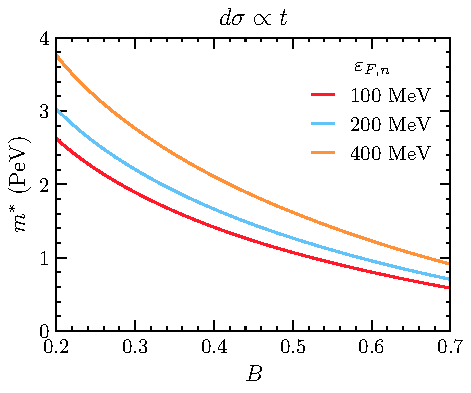
\includegraphics[width=.48\textwidth]{capture_1/mstar_B_n1.pdf}    
    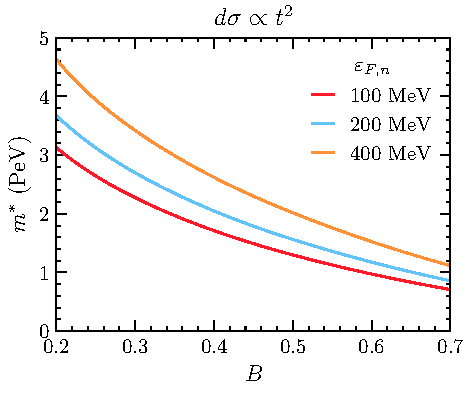
\includegraphics[width=.48\textwidth]{capture_1/mstar_B_n2.pdf}      
    \caption{Value of $m^*_n$ as a function of $B$ for different values of $\kinFn$, $\sigma=const.$ (top left), $d\sigma\propto t$ (top right) and $d\sigma\propto t^2$ (bottom).}
    \label{ch3:fig:mstarbmu}
\end{figure}
%%%%%%%%%%%%%%%%%%%%%%%%%%%%%%

When the cross-section is small, $\sigma\ll\sigmath$, such that we are in the optically thin regime, if the DM does not get captured in its initial scatter, then it will leave the star without interacting again. To account for this, the factor of $c_1$ should be included in the capture rate calculation, Eq.~\ref{ch3:eq:cap_rel_full_1}. However, as we have jsut seen, $c_1\ll1$ only for $\mchi\gtrsim\mstar$, which will always be significantly larger than the target mass and chemical potential. Therefore, multiple scattering is only important in the regime where PB is negligible, and so a suitable approximation for the capture rate in this regime is
\begin{equation}
    C_\mathrm{approx}^* = \frac{4\pi}{\vstar}\frac{\rho_\chi}{m_\chi}{\rm Erf}\left(\sqrt{\frac{3}{2}}\frac{\vstar}{v_d}\right)  \int  r^2 dr  \frac{\sqrt{1-B(r)}}{B(r)}\Omega^{-}(r) c_1(r),
    \label{ch3:eq:capturesimplelargem}
\end{equation}
with $\Omega^-(r)$ calculated as outlined in sections~\ref{ch3:subsec:captureintermediate}
    
% %%%%%%%%%%%%%%%%%%%%%%%%%%%%%%%%%%%%%
% %%%%%%%%%%%%%%%%%%%%%%%%%%%%%%%%%%%%%
\section{Results}
\label{ch3:sec:results}
% %%%%%%%%%%%%%%%%%%%%%%%%%%%%%%%%%%%%%
% %%%%%%%%%%%%%%%%%%%%%%%%%%%%%%%%%%%%%


In this section, we present our results for the capture rate of fermionic DM scattering from neutrons within a NS in the zero temperature approximation. We calculate the capture rate only for scalar/pseudoscalar-scalar/pseudoscalar interactions between DM and neutrons, i.e. effective operators D1-D4 in Table~\ref{ch1:tab:opers_defn_full}, whose differential cross-sections depend only on the Mandelstam variable $t$ and not on $s$. 
We use realistic radial profiles for the neutron number density, chemical potential, and relativistic corrections encoded in $B(r)$ as explained in Section~\ref{ch2:subsec:NS_EoS}, obtained from the BSk24 EoS for the configurations in Table~\ref{ch2:tab:BSk_configs}. 



% Most of our results apply generally to other operators or to other targets (with the mass ranges adjusted appropriately).  Specifically, Eqs.~\ref{eq:captureclsimplrel},~\ref{eq:omegampaulitext}, which are to be evaluated numerically, are applicable to all operators and targets, and work until multiple scattering becomes relevant, when $m_\chi\gtrsim \qomax/v_{\star}^2$.
% The optical factor of Eq.~\ref{eq:optfactor} for the intermediate mass range is also applicable to all operators and targets. The optical factor of Eq.~\ref{eq:optfactorlargem} and the value of $m^*$, which are used to include multiple scattering effects in the large mass range, $m_\chi\gtrsim \qomax/v_{\star}^2$, can be easily computed for operators D1-D4 (or any other operator that depends only on $t$) for all targets. For other operators it can be used only by numerically solving the shape of the differential rate, a task that may be computationally intensive to achieve with high precision.
% Our approximated formulas, Eqs.~\ref{eq:csimplelargemtext},~\ref{eq:capturesimplelargem} and \ref{eq:captureopticaldepth} have been checked to be accurate only for nucleon targets, but can be applied to any operator (for $s$-dependent ones, see Appendix~\ref{sec:capratesimple} on how to remove the $s$ dependence). In any case, one can substitute the relevant factors ($\eta,m^*$) into Eqs.~\ref{eq:captureclsimplrel},~\ref{eq:omegampaulitext} to calculate the capture rate, in the appropriate mass range, for other targets.




To estimate the NS EoS impact on the DM capture rate computation, we numerically calculate $C$ using the exact expression in the optically thin limit, Eq.~\ref{ch3:eq:capturefinalM2}, that properly accounts for gravitational focusing and Pauli blocking.  In the optically thin regime that we are working in, the capture rate is proportional to the differential DM-neutron cross-section. 
Fig.~\ref{ch3:fig:captureEOS} shows how this rate varies with the NS  EoS for operators D1-D4 and the EoS configurations given in Table~\ref{ch2:tab:BSk_configs}, and in turn with the NS mass and radius. 
The cross-section is normalised such that the capture rate in the intermediate mass range, which is unaffected by PB and multiple scattering, is equal to the geometric limit. It is worth remarking that cross-sections larger than the threshold cross-section should not be used in the optically thin limit, as this would result in capture rates larger than the geometric limit. To account for such large cross-sections, the optical depth of the NS must be accounted for as prescribed in Ref.~\cite{Bell:2020jou_sep_ImprovedTreatmentDark}.
Depending on the operator considered, going from the lightest to the heaviest NS can change the capture rate by a minimum of one order of magnitude, such as in the case of operators D1, D2 and D3 (at low DM mass), and up to 2 orders of magnitude, as in the case of operators D2 for large DM mass, and D4 in general. 

%%%%%%%%%%%%%%%%%%%%%%%%%%%%%%
\begin{figure}[t!bp]
    \centering
    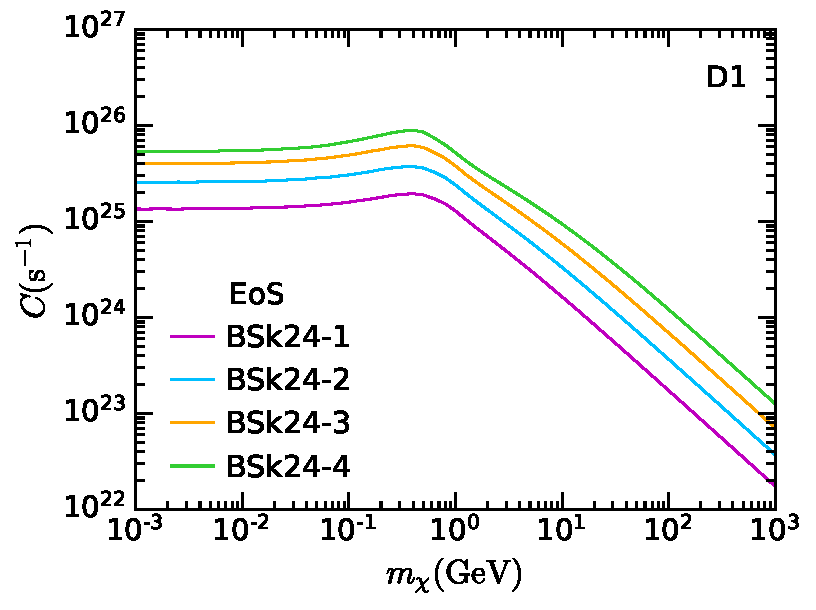
\includegraphics[width=.45\textwidth]{capture_1/capture_rate_numeric_EOS_D1.pdf}
    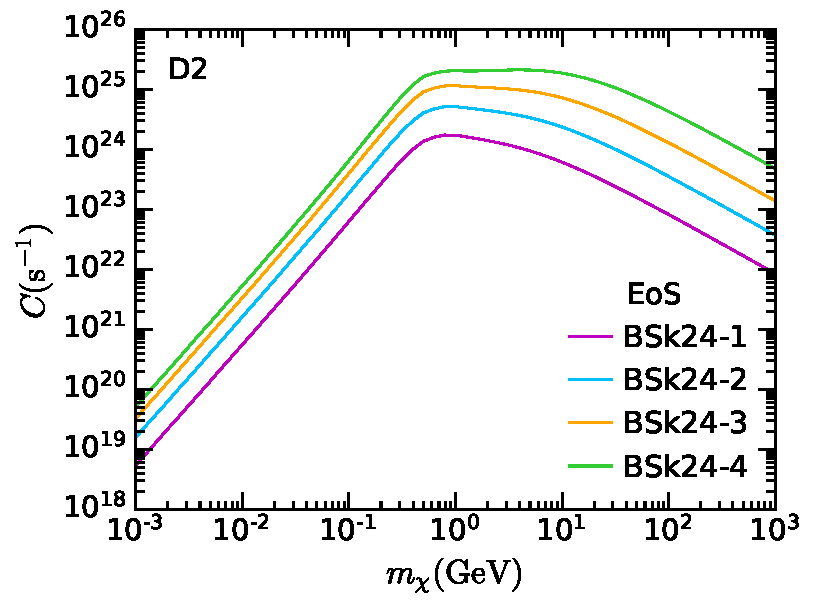
\includegraphics[width=.45\textwidth]{capture_1/capture_rate_numeric_EOS_D2.pdf}\\
    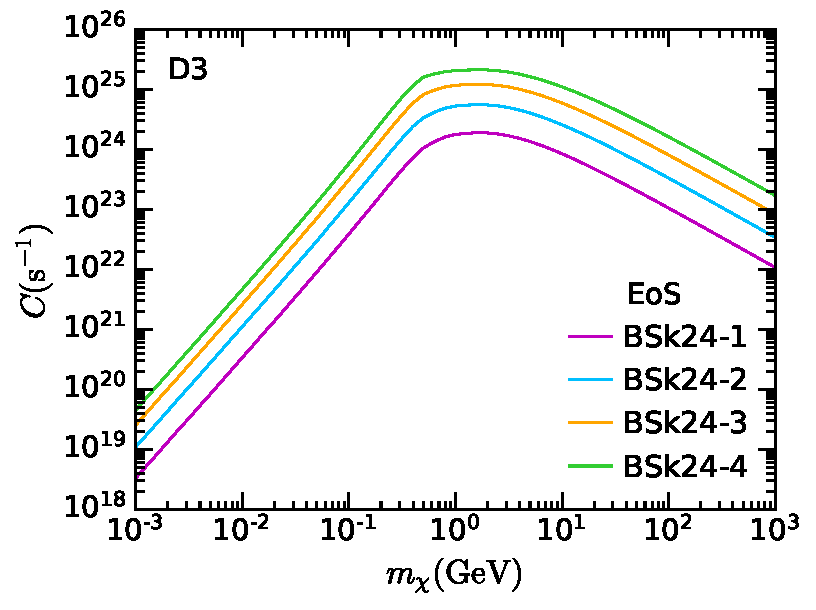
\includegraphics[width=.45\textwidth]{capture_1/capture_rate_numeric_EOS_D3.pdf}
    \includegraphics[width=.45\textwidth]{capture_1/capture_rate_numeric_EOS_D4.pdf}
    \caption[Capture rate in the optically thin limit as a function of the DM mass for $\sigma=\sigmaref\sim 1.7 \times 10^{-45} \cm^2$ and the configurations of the EoS BSk24 given in Table~\ref{ch2:tab:BSk_configs}.]{Capture rate in the optically thin limit as a function of the DM mass for $\sigma=\sigmaref\sim 1.7 \times 10^{-45} \cm^2$ and the configurations of the EoS BSk24 given in Table~\ref{ch2:tab:BSk_configs}. Rate calculated using the 4-dimensional integral in Eq.~\ref{ch3:eq:capturefinalM2}, that includes Pauli blocking but neglects the NS opacity and multiple scattering. Results are shown for the EFT operators D1 (top left), D2 (top right), D3 (bottom left) and D4 (bottom right) in Table~\ref{ch1:tab:opers_defn_full}.}
    \label{ch3:fig:captureEOS}
\end{figure}
%%%%%%%%%%%%%%%%%%%%%%%%%%%%%%




At large DM mass, all operators show the same scaling with the DM mass. At  $m_\chi\lesssim1\GeV$, a different picture arises as Pauli blocking leads to different suppressions of the capture rate for the different operators. However, we observe that the four operators give very similar results to those of Fig.~\ref{ch3:fig:approxc}, where we analysed the dependence of the capture rate on the momentum transfer $t$.  We note that operator D1, which contains in its squared matrix element a term independent of $t$, gives a result that is very similar to that of $\sigma=\mathrm{const}$. Operators D2 and D3, for which $\Msq$ does not include terms independent of $t$, but rather terms proportional to $t$ and $t^2$, yield very similar results to that of $d\sigma\propto t$. 
Overall, we conclude that the lowest power of the transferred momentum determines the mass scaling of the capture rate at low DM  mass.
This result holds true for matrix elements that depend also on $s$. 


%%%%%%%%%%%%%%%%%%%%%%%%%%%%%%
\begin{figure}[t!bp]
    \centering
    \includegraphics[width=.48\textwidth]{capture_1/capture_rate_n0_fullmassrange.pdf}    
    % \includegraphics[width=.48\textwidth]{capture_1/capture_rate_n0_largemass.pdf} %\\
    \includegraphics[width=.48\textwidth]{capture_1/capture_rate_n1_fullmassrange.pdf}       
    % \includegraphics[width=.48\textwidth]{capture_1/capture_rate_n1_largemass.pdf} \\
    \includegraphics[width=.48\textwidth]{capture_1/capture_rate_n2_fullmassrange.pdf}       
    % \includegraphics[width=.48\textwidth]{capture_1/capture_rate_n2_largemass.pdf}        
    \caption[Capture rate for constant cross-section (top left), $d\sigma\propto t$ (top right) and $d\sigma\propto t^2$ (bottom),  for  $\sigma=\sigmaref\sim 1.7 \times 10^{-45}\cm^2$ and NS EoS configuration BSk24-2.]{Capture rate for constant cross-section (top left), $d\sigma\propto t$ (top right) and $d\sigma\propto t^2$ (bottom),  for  $\sigma=\sigmaref\sim 1.7 \times 10^{-45}\cm^2$ and NS EoS configuration BSk24-2. These plots extent the mass range of those in Fig.~\ref{ch3:fig:approxc} to large DM masses.
    }
    \label{ch3:fig:capturelargemass}
\end{figure}
%%%%%%%%%%%%%%%%%%%%%%%%%%%%%%

In Fig.~\ref{ch3:fig:capturelargemass}, we show the capture rate for a broad DM mass range, spanning 13 orders of magnitude from $m_\chi=10\keV$ to $m_\chi=10^8\GeV$, including all three of the mass regimes we have discussed in the previous sections, for $d\sigma\propto const.$ (first row), $t^1$ (second row) and $t^2$ (third row).
The orange line indicates the capture rate calculated in the optically thin limit using the 4-dimensional integration in Eq.~\ref{ch3:eq:capturefinal} that accounts for Pauli blocking. 
At large DM masses, Pauli suppression plays no role and the capture rate approaches the geometric limit (dashed red line). 
We also show in Fig.~\ref{ch3:fig:capturelargemass} the effect of the inclusion of multiple scattering in the light blue line, which becomes relevant at $m_\chi\sim10^6\GeV$. 
% The difference among these calculations is better shown in the right panels, where only the large DM mass range is considered. The brown dashed line indicates the result that includes the optical depth factor $\eta$ but neglects multiple scattering, obtained using Eq.~\ref{eq:optfactor} in Eq.~\ref{eq:captureopticaldepth}.   
% As we can see, for $\sigma=\sigmaref$ this causes a small suppression of the capture rate, when compared to the result where the optical depth factor is ignored (light blue dot dashed line). For larger $\sigma$, neglecting the optical depth would result in a capture rate that exceeds the geometric limit (orange dashed line), while the inclusion of the optical depth factor $\eta$ causes the capture rate to saturate, tending to  $C_{geom}$ for large cross-sections. 
% The light blue dot dashed line indicates the capture rate calculated by neglecting the optical depth factor, but including multiple scattering, given by Eq.~\ref{eq:capturesimplelargem}. 
At $m_\chi\sim 10^5\GeV$ that line matches the geometric limit as expected from the chosen value of the cross-section $\sigma=\sigmaref$. At larger DM masses, $m_\chi\gtrsim10^6\GeV$, multiple scatterings are required for the DM to be captured, hence an additional suppression factor of $1/m_\chi$ arises, as given in Eq.~\ref{ch3:eq:capturesimplelargem}. Therefore, the capture rate becomes increasingly smaller than $C_{geom}$ (light blue shaded area). 
% Finally, the capture rate calculated including both effects is depicted in blue. At $m_\chi\sim10^5\GeV$, we can observe the suppression produced by the optical depth factor $\eta$ (light blue shaded region), while at larger DM masses the proper additional suppression $1/m_\chi$ emerges. 

Comparing the plots for different $t^n$ dependence, we can see that increasing the power of $n$ has a small effect on the mass scale where the various suppressions become relevant. For example, comparing the light blue lines between the three figures, we see that the change of slope from the onset of multiple scattering moves slightly further to the right for larger $n$. This is a consequence of the fact that larger powers of $n$ result in larger energy transfer (see, for example, Fig.~\ref{app:fig:diffgamma}), leading to a larger capture probability $c_1$ and hence a larger $\mstar$.
However, the qualitative behaviour is the same for all choices of $d\sigma$: the suppression of the capture rate is primarily due to Pauli blocking at low mass and multiple scattering effects (i.e. a low capture probability) at large masses.


%%%%%%%%%%%%%%%%%%%%%%%%%%%%%%%%%%
%%%%%%%%%%%%%%%%%%%%%%%%%%%%%%%%%%
\section{Summary}
\label{ch3:sec:conclusion}
%%%%%%%%%%%%%%%%%%%%%%%%%%%%%%%%%%
%%%%%%%%%%%%%%%%%%%%%%%%%%%%%%%%%%


In this chapter, we have improved and extended the existing framework used to calculate the DM capture rate in the Sun to be compatible with compact objects, relaxing the simplifying assumptions that have previously been made. Specifically, we have derived exact expressions for the capture rate that correctly incorporate relativistic kinematics, gravitational focusing, Pauli blocking, and multiple-scattering effects. We also properly incorporate the internal structure of the star, consistently calculating the radial profiles of the EoS-dependent parameters and the general relativistic corrections, by solving the Tolman-Oppenheimer-Volkoff equations.

This new formalism was applied to neutron stars to highlight the features of the formalism mentioned above.
Neutron stars (and compact objects in general) are composed of strongly degenerate matter, resulting in significant Pauli blocking of scattering interactions when the dark matter is light, $m_\chi\lesssim \mi$, suppressing the capture rate by several orders of magnitude. By including the radial dependence of the chemical potential in our calculations, we correctly account for Pauli suppression at any point in the star. However, note that the chemical potential is dependent on the EoS assumption.


For very large DM masses, $m_\chi\gtrsim10^6\GeV$, the energy lost in a single collision will be insufficient for it to be captured. Hence, the DM must scatter multiple times within an orbit to be captured, or else it simply leaves the star. To correctly compute the DM capture probability due to multiple scattering, we have derived, for the first time, an exact equation for the DM interaction rate in degenerate matter, and used that result to compute the differential capture rate as a function of the DM energy loss. This enables us to compute the cumulative probability that a DM particle is captured after multiple interactions, by averaging over the initial DM velocity distribution.


Although we have framed our results in terms of the scattering of DM from neutron targets in neutron star, it is straightforward to obtain the capture rate for DM scattering from any other degenerate species in compact objects. In the next chapter, we apply this formalism to DM scattering off the leptonic compoennts of NSs, as well as the degenerate electrons within WDs.


  %% Capture on leptons: NS and WD
  \graphicspath{{img/capture_leptons/}}
%%%%%%%%%%%%%%%%%%%%%%%%%%%%%%%%%%%%%
%%%%%%%%%%%%%%%%%%%%%%%%%%%%%%%%%%%%%
%%%%%%%%%%%%%%%%%%%%%%%%%%%%%%%%%%%%%

\chapter{Dark Matter Capture from Leptonic Species}
\label{chapter:capture_leptons}

\begin{synopsis}
This chapter is based on the results of Ref.~\cite{Bell:2020lmm_mar_ImprovedTreatmentDark} and on the electron capture resluts in Ref.~\cite{Bell:2021fye_oct_Improvedtreatmentdark}. We apply the formalism for capture in compact objects to leptonic targets in neutron stars and white dwarfs. In NSs, we calculate the projected sensitivities for the threshold DM-electron/muon cross-sections that could be probed in future observations. We then move to capture from the electrons in WDs, where we analyse the existing observations of the WDs in the globular cluster M4. Limits are placed on the DM-electron cross-section by requiring that the DM does not heat up the WDs above their observed temperatures through scattering and annihilation.
\end{synopsis}
%%%%%%%%%%%%%%%%%%%%%%%%%%%%%%%%%%%%%
%%%%%%%%%%%%%%%%%%%%%%%%%%%%%%%%%%%%%
%%%%%%%%%%%%%%%%%%%%%%%%%%%%%%%%%%%%%


%%%%%%%%%%%%%%%%%%%%%%%%%%%%%%%%%%%%%
%%%%%%%%%%%%%%%%%%%%%%%%%%%%%%%%%%%%%

\section{Capture from Leptons in Neutron Stars}
\label{ch4:sec:lep_NS}
%%%%%%%%%%%%%%%%%%%%%%%%%%%%%%%%%%%%%
%%%%%%%%%%%%%%%%%%%%%%%%%%%%%%%%%%%%%
Despite NSs being composed primarily of baryons (neutrons and protons in particular), they can still contain a substantial number of leptonic particles, namely electrons and, to a smaller extent, muons. For example, 1.5 $\Msun$ NS can contain $\sim 5\times 10^42$ leptons, corresponding to a threshold cross-section $\sigmathl\sim 10^{-43}\cm^2$, far below current direct detection bounds. This warrents a detailed study into the DM-lepton parameter space that could be explored with upcoming NSs observations. 

To that end, we will consider the BSk24 EoS, with the benchmark configurations listed in Table.~\ref{ch2:tab:BSk_configs}.
In Fig.~\ref{ch4:fig:NSradprofs1} we plot the corresponding lepton profiles.
As mentioned above, electrons are present in the core and the crust while muons appear at baryon number densities $n_b\simeq 0.12\fm^{-3}$. The kink observed in the electron chemical potential marks out the transition from the core to the inner crust. 
The aforementioned radial profiles will be used in the following section to calculate the capture rate. 

\begin{figure}[t] 
    \centering
    \includegraphics[width=0.495\textwidth]{capture_2/NS_ne_r_BSk24.pdf}
    \includegraphics[width=0.495\textwidth]{capture_2/NS_MuFe_r_BSk24.pdf}
    \includegraphics[width=0.495\textwidth]{capture_2/NS_nmu_r_BSk24.pdf}
    \includegraphics[width=0.495\textwidth]{capture_2/NS_MuFmu_r_BSk24.pdf}
    \caption{Number density profile (left) and chemical potential (right) for electrons (top) and muons (bottom) and NS configurations of the  BSk24 functional in Table~\ref{ch2:tab:BSk_configs}. 
    }
    \label{ch4:fig:NSradprofs1}
\end{figure}



%%%%%%%%%%%%%%%%%%%%%%%%%%%%%%%%%%%%%%%%%%%%%%%%%%%%%%%%%%%%%%%%%%%%%%%%%%%%%%%%%%%%
%%%%%%%%%%%%%%%%%%%%%%%%%%%%%%%%%%%%%%%%%%%%%%%%%%%%%%%%%%%%%%%%%%%%%%%%%%%%%%%%%%%%
\subsection{Capture Rate}
\label{ch4:subsec:caprateresults}
%%%%%%%%%%%%%%%%%%%%%%%%%%%%%%%%%%%%%%%%%%%%%%%%%%%%%%%%%%%%%%%%%%%%%%%%%%%%%%%%%%%%
%%%%%%%%%%%%%%%%%%%%%%%%%%%%%%%%%%%%%%%%%%%%%%%%%%%%%%%%%%%%%%%%%%%%%%%%%%%%%%%%%%%%

In this section, we present results for the capture rate $C\Lambda^4$ for each of the EFT operators in Table~\ref{ch1:tab:opers_defn_full}, calculated in the optically thin limit using Eq.~\ref{ch3:eq:capturefinalM2} for $m_\chi\lesssim m_\ell^*$ and  Eq.~\ref{ch3:eq:capturesimplelargem} for $m_\chi\gtrsim m_\ell^*$\footnote{To numerically solve these equations we use the \texttt{CUBA} libraries \cite{Hahn:2004fe_CUBALibrarymultidimensional, Hahn:2014fua_Concurrentcuba} linked to \texttt{Mathematica}~\cite{Mathematica}.}. Typical values of $m_\ell^\star$ and $\sigmathl$ are shown in Table.~\ref{ch4:tab:mstarsigma} for electron and muon targets. Note that in $m_\ell^*$ will depend on the values of $B(r)$ and $\kinFl(r)$, as well as the type of interaction considered. 

\begin{figure}[t] 
    \centering
    \includegraphics[width=\textwidth]{capture_2/D1_D4_C_mDM_lept.pdf}
    \caption{Capture rate in the optically thin limit for operators D1-D4 as a function of the DM mass $m_\chi$ for electrons (light blue) and muons (magenta) in the NS benchmark models BSk24-1 (dashed), BSk24-2 (solid) and BSk24-4 (dot-dashed). The shaded regions denote the change in the capture rate with the NS configuration for the same EoS family BSk24. 
    All capture rates scale as $\Lambda^{-4}$. We require $\Lambda$ to be sufficiently large that the capture rates are smaller than the geometric limit, $C_\mathrm{geom}$. 
    }
    \label{ch4:fig:capratesD1D4}
    \end{figure} 
    
     \begin{figure}[t!bp] 
    \centering
    \includegraphics[width=\textwidth]{capture_2/D5_D10_C_mDM_lept.pdf}
    \caption{Capture rate in the optically thin limit for operators D5-D10 as a function of the DM mass $m_\chi$ for electrons (light blue) and muons (magenta) in the NS benchmark models BSk24-1 (dashed), BSk24-2 (solid) and BSk24-4 (dot-dashed). All capture rates scale as $\Lambda^{-4}$. The shaded regions depict the difference between capture by electrons and muons for the above mentioned NS models. 
    }
    \label{ch4:fig:capratesD5D10}
    \end{figure}

    

Figs.~\ref{ch4:fig:capratesD1D4} and~\ref{ch4:fig:capratesD5D10} show the results for electron (light blue) and muon (magenta) targets, considering three NS benchmark models: BSk24-1 (dashed, $1\Msun$), BSk24-2 (solid, $1.5\Msun$) and BSk24-4 (dot-dashed, $2.16\Msun$). In addition, we assume a nearby NS, located in the Solar neighbourhood, and thus take $\rho_\chi=0.4\GeV\cm^{-3}$, $\vstar=230\km\s^{-1}$ and $v_d=270\km\s^{-1}$.  

\begin{table}[t!bp]
    \centering
    \begin{tabular}{l c c}
    \toprule
    \bf Target & $\bm{\mu}$ & $\bm{e}$  \\
    \midrule
    $m_\ell^*\; (\GeV)$  & $[0.3,3] \times 10^{5}$ & $[0.05,1.7] \times 10^{5}$  \\
    $\sigmathl\; (\cm^2)$ &  $8\times 10^{-44}$ & $3\times 10^{-44}$ \\
    \bottomrule
    \end{tabular} 
    \caption{Typical values of $m_\ell^*$ and $\sigmathl$ for lepton targets. 
    The exact value of $\sigmathl$ depends on the DM mass, and the operator. We show  here the simplest case of constant matrix element; other operators give similar results. The threshold cross section is approximately constant in the range $1\GeV\lesssim m_\chi\lesssim m_\ell^*$, and takes larger values outside that range with a $1/m_\chi$ or $m_\chi$ scaling for small and large masses, respectively. }
    \label{ch4:tab:mstarsigma}
    \end{table} 

In these figures, we observe that the capture rate is suppressed due to Pauli blocking when $m_\chi \lesssim m_\ell$. The change of slope at $m_\chi\sim m_\ell^* \sim 10^5\GeV$, observed for both targets, is due to multiple scattering. 
For the operators D5-10 (Fig.~\ref{ch4:fig:capratesD5D10}), whose matrix elements depend explicitly on $s$,  the slope of the capture rate in the three mass regimes are all very similar to one another, while for D1-D4 (Fig.~\ref{ch4:fig:capratesD1D4}), the shape of $C$ is controlled by the power of $t$ that dominates the interaction, which in general is the lowest power \cite{Bell:2020jou_sep_ImprovedTreatmentDark}. 

The exceptions to this are the capture rates for operators D1 and D2 with electron targets, which show a distinctive feature in the region $m_e\lesssim m_\chi\lesssim 100\MeV$ that does not occur for the other operators.  
The capture rate for D1 and D2 is more suppressed in that particular region, similarly to D3 and D4, respectively. This is due to the form of the corresponding matrix elements together with the smallness of the electron mass. Namely, 
D1 and D2 are the only two operators that contain a factor $(t-4 m_\ell^2)$ in their scattering amplitudes, for electrons this means that the lowest power of $t$ in $\Msq$ is multiplied by $m_e^2$, i.e. these terms are suppressed in the $m_e \lesssim m_\chi\lesssim 100\MeV$ range. Consequently, the capture rate in that DM mass region is dominated by the unsuppressed $t$-terms  in $\Msq$, these being $t$  for D1 (as for D3) and $t^2$ for D2 (see Table~\ref{ch1:tab:opers_defn_full}), while below $m_e$ this additional suppression disappears and the capture rate follows the lowest power of $t$ as was originally expected. 

From Fig.~\ref{ch4:fig:capratesD1D4}, we note that for the same cutoff scale $\Lambda$, the muon contribution to the total capture rate for operators D1-D4 surpasses that of the electron by approximately 4 orders of magnitude for most of the DM mass range, and by about 8 orders of magnitude at very low mass for operators D1-D2. This is due to the large hierarchy between DM couplings to electrons and muons, which is of order $(\frac{m_\mu}{m_e})^2$. 
For operators D5-D10, electrons and muons will have the same strength couplings to DM (see Table~\ref{ch1:tab:opers_defn_full}). However, despite similar couplings and a lower abundance, muons are still able to capture DM at a rate comparable to electrons (see light blue regions in Fig.~\ref{ch4:fig:capratesD5D10}), thanks to their larger mass and lower chemical potential (see Fig.~\ref{ch4:fig:NSradprofs1}, right panels). This means that their interactions with DM are less Pauli suppressed, leading to a larger interaction rate. The small difference between the rates at which electron and muon are able to capture DM particles reduces for heavier NS configurations, e.g. from a factor $\sim5$ (BSk24-1) to $\sim 1.5$ (BSk24-4) for D6 and D10; see the light blue shaded regions in Fig.~\ref{ch4:fig:capratesD5D10}. This is due to the muon abundance increasing in heavier NSs.



It is also worth noting that different EoS assumptions can lead to variations in the capture rate for electron targets of at least two orders of magnitude in the Pauli suppressed region and $\sim 2.5$ orders of magnitude in the large DM mass regime (compare dashed with dot-dashed light blue lines). For muons, the effect is even larger, with capture rate variations from $\sim {\cal O}(5\times 10^2)$ for low DM mass to $\sim {\cal O}(2\times 10^3)$ for heavy DM, when comparing the lightest and most massive NS configurations of the BSk24 family. For the operators D2 and D4, these variations are even more pronounced for both electrons and muons and can reach  $\sim {\cal O}(5\times 10^3)$ and  $\sim {\cal O}(5\times 10^4)$, respectively for very large DM masses. 


\begin{figure}
    \centering
    \includegraphics[width=.7\textwidth]{capture_2/capture_rate_n0_comp_muons.pdf}
    \caption{ Capture rate in the optically thin limit for muon targets  (magenta) and geometric (orange) limit as a function of the DM mass for constant cross-section $\sigma_{\mu\chi}=10^{-45}\cm^2$,  $\rho_\chi=1\GeV\cm^{-3}$ and BSk26 functional for $\Mstar\simeq1.52\Msun$ and $\Rstar\simeq11.6\km$ denoted as BSk26-1. Capture rate calculations from Ref.~\cite{Garani:2018kkd_may_NewAnalysisNeutron} for a NS configuration with EoS BSk20-1~\cite{Potekhin:2013qqa_Analyticalrepresentationsunified} equivalent to BSk26-1, are shown for comparison. 
    }
    \label{ch4:fig:Cratecomp}
\end{figure}
  

The DM capture rate for muon targets was calculated in Ref.~\cite{Garani:2018kkd_may_NewAnalysisNeutron}, for constant cross-section and light DM, $m_\chi\leq10\GeV$. That calculation accounts for the NS internal structure and Pauli blocking, but neglects general relativity (GR) corrections and assumes that muons are non-relativistic. 
As outlined in Section~\ref{ch3:subsec:captureintermediate}, to compare our capture rate calculation with that of Ref.~\cite{Garani:2018kkd_may_NewAnalysisNeutron}  we select a NS model that matches that of Fig.~12 of Ref.~\cite{Garani:2018kkd_may_NewAnalysisNeutron}, namely Model A (BSk20-1):  $\Mstar\simeq1.52\Msun$, $\Rstar\simeq11.6\km$. This new benchmark model is denoted as BSk26-1.  

In Fig.~\ref{ch4:fig:Cratecomp}, we compare both capture rate calculations for  $\sigma_{\mu\chi}=10^{-45}\cm^2$ and the same assumptions about $\rho_\chi$, $v_\star$ and $v_d$ as in Ref.~\cite{Garani:2018kkd_may_NewAnalysisNeutron}. Comparing the geometric limit, Eq.~\ref{ch3:eq:capturegeom}  (solid orange), which properly accounts for gravitational focusing in NSs, with the non-relativistic computation in Ref.~\cite{Garani:2018kkd_may_NewAnalysisNeutron} (dot-dashed brown), we observe a $\sim 67 \%$ enhancement, due to the $1/B(\Rstar)$ factor that encodes GR corrections~\cite{Goldman:1989nd_WeaklyInteractingMassive,Kouvaris:2007ay_WIMPAnnihilationCooling}. 
In the region not affected by Pauli blocking, $m_\chi \gtrsim m_\mu$, our calculation in the optical thin limit (solid magenta) exceeds that of Ref.~\cite{Garani:2018kkd_may_NewAnalysisNeutron} (dot-dashed blue) by a factor of $\sim 4$, which increases as we move to the Pauli suppressed region where our computation is more than one order of magnitude higher. Unlike Ref.~\cite{Garani:2018kkd_may_NewAnalysisNeutron}, our formalism incorporates GR corrections and made use of relativistic kinematics. We also show in dashed light blue, an estimation of the capture rate using the approximation $\delta p/p_{F,\mu}\sim m_\chi v_{esc}/p_{F,\mu}$  for $m_\chi < m_\mu$~\cite{McDermott:2011jp_ConstraintsScalarAsymmetric}, where $p_{F,\mu}$ is the muon Fermi momentum and $v_{esc}$ is the escape velocity. This approximation overestimates the capture rate by a factor of approximately 2 in the Pauli blocked region below 10 MeV and underestimates it in the region of larger DM masses. 





%%%%%%%%%%%%%%%%%%%%%%%%%%%%%%%%%%%%%%%%%%%%%%%%%%%%%%%%%%%%%%%%%%%%%%%%%%%%%%%%%%%%
\subsection{Finite Temperature Effects and Evaporation}
\label{ch4:subsec:finite_temp_NS}
%%%%%%%%%%%%%%%%%%%%%%%%%%%%%%%%%%%%%%%%%%%%%%%%%%%%%%%%%%%%%%%%%%%%%%%%%%%%%%%%%%%%



In Section~\ref{ch4:subsec:caprateresults}, we have restricted our computation of the capture rates to the DM mass range $m_\chi\in[1\keV,10^8\GeV]$. While the upper limit on this mass range is somewhat arbitrary, primarily limited by the increasing numerical tax of calculating Eq.~\ref{ch3:eq:capturesimplelargem}, the lower bound comes from working in the zero-temperature approximation, $\Tstar \rightarrow 0$. This approximation is valid for DM masses $\mchi \gg\Tstar$, which for a $10^3\K$ star requires $\mchi \gg 90$ meV.

For DM masses $m_\chi\lesssim \mathcal{O}(10)\Tstar$, thermal effects begin to play an important role in the capture rate, significantly boosting the rate in this low mass range~\cite{Garani:2018kkd_may_NewAnalysisNeutron}. Consequently, the complete Fermi-Dirac distributions should be used in Eqs.~\ref{ch3:eq:scattrate} and~\ref{ch3:eq:int_rate_capture_full}. To illustrate the effect of the NS temperature,  we show in Fig.~\ref{ch4:fig:CfiniteT_e} the ratio of the capture rate in a NS with 
$\Tstar=10^5\K\simeq8.6\eV$ to the corresponding capture rate in the $\Tstar\rightarrow0$ limit, assuming scattering on electrons, the targets for which this effect is most relevant. 

From this figure, we immediately notice that the ratio starts to depart from  $1$ at $m_\chi\sim100\eV\sim 10T_\star$ for all operators. Operators whose matrix element depends on higher powers of the exchanged momentum  $t$ feature a larger increment in the capture rate due to finite temperature. In fact, the operator D4 ($|\overline{M}|^2\propto t^2$) receives the largest correction, followed by D2-D3 (whose $|\overline{M}|^2$ is a linear combination of $t^1,t^2$), then D1 ($|\overline{M}|^2$ is a linear combination of $t^0,t^1,t^2$) and finally by  D5-D10 (whose $|\overline{M}|^2$ include all powers of the kind $t^n s^m$).

\begin{figure}[t!bp]
    \centering
    \includegraphics[width=0.7\textwidth]{capture_2/R_CT_mdm_10_5K_D1_D10_e.pdf}
    \caption{Finite temperature effects on the capture rate for electron targets, assuming the NS model BSk24-2. The DM mass range where capture and evaporation are expected to be in equilibrium is shaded in yellow. The dashed brown line corresponds to the evaporation mass.}
    \label{ch4:fig:CfiniteT_e}
\end{figure}


In the very light DM regime, there is another that needs to be accounted for: evaporation. This occurs when the dark matter up-scatters to a state where the final DM kinetic energy is larger than the energy required to escape the star, and hence DM particles are expelled. Thus, as opposed to capture, evaporation drains energy from the star. 
To estimate the evaporation rate, we convolve the DM distribution within the star, with the interaction rate for up-scattering, $\Gamma^-_\mathrm{up}(E_\chi, \Tstar)$, retaining the temperature dependence.

Assuming the DM distribution to be isothermal with temperature $T_\chi=\Tstar$, we have 
\begin{align}
n_\chi^\mathrm{iso}(r,E_\chi) &= \frac{n_c}{1+e^{\frac{E_\chi-m_\chi\left(\frac{1}{\sqrt{B(r)}}-1\right)}{\Tstar}}} \\
& \simeq \frac{ \exp\left[-\frac{E_\chi-m_\chi\left(\frac{1}{\sqrt{B(r)}}-1\right)}{\Tstar}\right]}{4\pi \int_0^{\Rstar} dr r^2  \int_0^{m_\chi\left(\frac{1}{\sqrt{B(r)}}-1\right)} dE_\chi \exp \left[{-\frac{E_\chi-m_\chi\left(\frac{1}{\sqrt{B(r)}}-1\right)}{\Tstar}}\right]}, 
\end{align}
where $n_c$ is a normalisation constant such that the total number of DM particles is $N_\chi = \int d^3r\int dE_\chi\;n_\chi^\mathrm{iso}(E_\chi, r)$. The interaction rate for up-scattering, $\Gamma^-_\mathrm{up}(E_\chi, \Tstar)$ can be related to the down-scattering rate through
\begin{equation}
\frac{d\Gamma^-_\mathrm{up}}{dq_0}\left(E_\chi, q_0,\Tstar\right) = -\frac{e^{q_0/\Tstar}}{1-e^{q_0/\Tstar}} \dfrac{d\Gamma^-}{dq_0}\left(E_\chi, q_0\right),\quad q_0<0,
\label{ch4:eq:upscattintrate}
\end{equation}
where $\tfrac{d\Gamma^-}{dq_0}$ is the differential interaction rate in the $\Tstar\rightarrow 0$ approximation derived in Appendix~\ref{app:subsec:down_scatter_derivation}, with the full derivation of Eq.~\ref{ch4:eq:upscattintrate} in Appendix~\ref{app:subsec:up_scatter_derivation}. 

The evaporation rate then reads
\small
\begin{align}
E &\simeq 4\pi \int_0^{\Rstar} dr r^2 \int_0^{m_\chi\left(\frac{1}{\sqrt{B(r)}}-1\right)}dE_\chi n_\chi^\mathrm{iso}(r,E_\chi) \int_{-\infty}^{-q_0^\mathrm{min}} dq_0 \frac{d\Gamma^-_\mathrm{up}}{dq_0}\left(q_0,\Tstar\right), \\
q_0^\mathrm{min} & = m_\chi\left(\frac{1}{\sqrt{B(r)}}-1\right)-E_\chi,
\label{ch4:eq:evaprate}
\end{align}
\normalsize
where $q_0^\mathrm{min}$ is the minimum energy the DM needs to gain to be ejected from the star.
When the DM distribution is concentrated very close to the centre of the star, this expression can be approximated by
\begin{equation}
E \sim  \frac{ m_\chi m_\ell^2\sigma_{\ell\chi}}{4\pi^2} \left(\frac{1}{\sqrt{B(0)}}-1\right)^2  \exp\left[{-\frac{m_\chi}{\Tstar}}\left(\frac{1}{\sqrt{B(0)}}-1\right)\right]. \end{equation}

The rate at which DM particles accumulate in NSs is then given by
\begin{equation}
\dfrac{dN_\chi}{dt} = C- E N_\chi,
\end{equation}
assuming that DM annihilation is negligible. The solution of this equation is 
\begin{equation}
N_\chi(\tstar) = C \, \tstar \left( \frac{ 1-e^{-E \, \tstar}}{E \, \tstar} \right),   
\end{equation}
where $\tstar$ is the age of the NS. The term in brackets quantifies the depletion of the number of capture DM particles due to the evaporation process. This factor will be of order 1 unless $E(m_\chi) \, t_\star \gtrsim {\cal O}(1)$. Therefore, we will define the evaporation mass as the DM mass for which the previous relation holds, i.e.  $E(m_\mathrm{evap}) t_\star \sim 1$. 
For DM masses below this threshold, $m_\chi \lesssim m_\mathrm{evap}$, the capture and evaporation processes are in equilibrium with each other. In that limit, the net energy exchange in the star due to the combined effects of DM capture and evaporation would be negligible, and hence we would be unable to constrain DM interactions using the NS temperature as a probe.


Using Eq.~\ref{ch4:eq:evaprate}, we find the evaporation mass to be of order $m_\mathrm{evap}\sim\mathcal{O}(100\Tstar)$ for all scattering targets in old NSs with $\tstar\sim{\cal O}(10 \Gyr)$. For instance, for $\Tstar=10^5\K$ and electron targets, we obtain $m^e_\mathrm{evap}\simeq 300\eV$. 
The region in Fig.~\ref{ch4:fig:CfiniteT_e} for which capture and evaporation are in equilibrium is shaded in yellow, with the evaporation mass indicated by the dashed brown line. From this, we can see that the finite temperature effects on the capture rate come become importatnt for masses below the evaporation mass, for all operators we consider. Hence, when calculating the capture rate while aiming to constrain DM interactions, finite temperature effects can be safely neglected.



%%%%%%%%%%%%%%%%%%%%%%%%%%%%%%%%%%%%%%%%%%%%%%%%%%%%%%%%%%%%%%%%%%%%%%%%%%%%%%%%%%%%
%%%%%%%%%%%%%%%%%%%%%%%%%%%%%%%%%%%%%%%%%%%%%%%%%%%%%%%%%%%%%%%%%%%%%%%%%%%%%%%%%%%%
\subsection{Results}
\label{ch4:subsec:results_NS}
%%%%%%%%%%%%%%%%%%%%%%%%%%%%%%%%%%%%%%%%%%%%%%%%%%%%%%%%%%%%%%%%%%%%%%%%%%%%%%%%%%%%
%%%%%%%%%%%%%%%%%%%%%%%%%%%%%%%%%%%%%%%%%%%%%%%%%%%%%%%%%%%%%%%%%%%%%%%%%%%%%%%%%%%%

%%%%%%%%%%%%%%%%%%%%%%%%%%%%%%%%%%%%%%%%%%%%%%%%%%%%%%%%%%%%%%%%%%%%%%%%%%%%%%%%%%%%
\subsubsection{Threshold Cross-Sections}
\label{ch4:subsubsec:thxs}
%%%%%%%%%%%%%%%%%%%%%%%%%%%%%%%%%%%%%%%%%%%%%%%%%%%%%%%%%%%%%%%%%%%%%%%%%%%%%%%%%%%%

In Section~\ref{ch3:subsec:geom_lim_threshold_xs}, we defined the threshold cross-section, $\sigmathl$, as the cross-section for which the capture rate, $C(\sigma(\Lambda),m_\chi)$, calculated in the optically thin regime becomes equal to the geometric limit, $C_\mathrm{geom}$. 
The threshold cross-section restricts the NS sensitivity to DM-target interactions since for $\sigma\ge\sigmathl$ the capture rate saturates to the geometric limit $C_\mathrm{geom}$. 



In Fig.~\ref{ch4:fig:sigmathe}, we show the threshold cross-sections for lepton targets, electrons and muons, and compare them with existing direct detection limits and expected sensitivities of future experiments. The neutrino floor for electron recoil experiments for silicon targets~\cite{Essig:2018tss_Solarneutrinossignal} is shown as a shaded yellow region.
The solid light blue and magenta lines correspond to the value of $\sigma_{th}$ for electrons and muons respectively, calculated using the NS model BSk24-2  ($1.5 M_\odot$), while the shaded bands in light blue and magenta denote the expected range for $\sigma_{th}$ for the two different targets, obtained by varying the NS configuration along the BSk24 family. 
 BSk24-1 ($1M_\odot$) gives the upper bound on $\sigmath$ and BSk24-4 ($2.16 M_\odot$) the lower bound. 
Note that the variation in $\sigmath$ due to the NS EoS increases with the DM mass and for muons goes from about one order of magnitude in the low mass range, to two orders of magnitude in the multiple scattering region. For electrons, this effect is slightly less pronounced.


    
All the limits for existing experiments are orders of magnitude weaker than the expected NS reach, with only the future DAMIC-M~\cite{Essig:2015cda_DirectdetectionsubGeV} (dashed brown line) expected to overcome NS electron scattering sensitivity and approach that of muons, in the DM mass range  $3\MeV\lesssim m_\chi\lesssim 30\MeV$. Moreover, NS sensitivity to DM interactions with lepton targets is expected to be well below the neutrino floor for $m_\chi\gtrsim 100\MeV$ and, in the case of muons, even for $m_\chi\lesssim 1\MeV$. 

\begin{figure}[t!bp]
    \centering
    \includegraphics[width=0.49\textwidth]{capture_2/DD_NS_leptons.pdf}
    \includegraphics[width=0.49\textwidth]{capture_2/DD_NS_leptons_D5.pdf}
    \caption{DM-lepton threshold cross-section for operators D1 (left) and D5 (right) for the EoS BSk24. The solid blue (electron) and magenta (muon) lines represent $\sigmath$, are computed assuming the NS model BSk24-2, while the shaded bands represent the expected range due to variation of the EoS. For comparison, we show leading electron recoil bounds for heavy mediators from SENSEI~\cite{SENSEI:2020dpa_oct_SENSEIDirectDetectionResults}, DAMIC~\cite{DAMIC:2019dcn_Constraintslightdark}, Xenon10~\cite{Essig:2017kqs_Newconstraintsprospects}, Xenon1T~\cite{XENON:2019gfn_Lightdarkmatter}, projected sensitivities from DAMIC-M~\cite{Essig:2015cda_DirectdetectionsubGeV} as well as the neutrino floor for silicon detectors~\cite{Essig:2018tss_Solarneutrinossignal}.}
        \label{ch4:fig:sigmathe}
\end{figure}

Note that NSs have a better sensitivity to vector-vector interactions (operator D5, see right panel) than scalar-scalar interactions (operator D1, see left panel) in the low DM regime for both leptonic targets, and especially for electrons. As discussed in Section~\ref{ch4:subsec:caprateresults}, there is an additional suppression in the capture rate of scalar operators that stems from an $m_e^2 \, t$ term in their scattering amplitudes. 

Similar threshold cross-sections can be estimated for the remaining operators.  Operators with s-dependent matrix elements (D6-D10) have  $\sigmath$ that behave like that of D5 for both electrons and muons. D2 presents the same features as D1 in the sub-GeV regime for electrons, due to the similar shape of their capture rates (see Fig.~\ref{ch4:fig:capratesD1D4}) and D3-D4 show a steeper slope in the $m_\chi\lesssim m_e$ region with respect to D1-D2, due to the capture rate dependence on higher powers of $t$. 



%%%%%%%%%%%%%%%%%%%%%%%%%%%%%%%%%%%%%%%%%%%%%%%%%%
\subsubsection{Comparison with Literature}
\label{ch4:subsubsec:literature_comp_NS}
%%%%%%%%%%%%%%%%%%%%%%%%%%%%%%%%%%%%%%%%%%%%%%%%%%

We now compare our calculations for the capture rates and resulting reach in the EFT cutoff $\Lambda$ for operators D1 and D5 to those presented in Refs.~\cite{Joglekar:2019vzy_sep_Relativisticcapturedark,Joglekar:2020liw_Darkkineticheating}\footnote{Note that the Yukawa couplings for scalar and pseudoscalar operators in Refs.~\cite{Joglekar:2019vzy_sep_Relativisticcapturedark,Joglekar:2020liw_Darkkineticheating} are embedded into the cutoff scale $\Lambda$.}.
The formalism in Refs.~\cite{Joglekar:2019vzy_sep_Relativisticcapturedark,Joglekar:2020liw_Darkkineticheating} is valid for relativistic and non-relativistic targets in a broad mass range, however, several simplifying assumptions were made that are accounted for in our results. Namely, they do not account for the DM velocity distribution far from the star, nor do they incorporate the internal structure of the NS. Instead, constant chemical potentials and particle abundances that have been averaged over the core volume are used. These quantities correspond to the NS model BSk24-2 and were calculated in Ref.~\cite{Bell:2019pyc_jun_CaptureLeptophilicDark}. 



\begin{figure}[t!bp]
    \centering
    \includegraphics[width=\textwidth]{capture_2/D1_Lambda_mdm_leptons.pdf}\\
    \vspace*{-0.5em}    
    \includegraphics[width=\textwidth]{capture_2/D1_C_mdm_leptons.pdf}     
    \caption{Comparison of the reach in $\Lambda$ for D1 with the approach of Ref.~\cite{Joglekar:2020liw_Darkkineticheating}. The shaded regions denote the difference in $\Lambda$ (top) and $C\Lambda^4$ (middle) between the two approaches and their ratio is shown in the bottom panels.}
    \label{ch4:fig:D1_Lambda_mdm}
\end{figure}


    
In the top panels of Figs.~\ref{ch4:fig:D1_Lambda_mdm} and~\ref{ch4:fig:D5_Lambda_mdm}, we compare the reach in $\Lambda$ for DM-lepton scattering cross-sections in Refs.~\cite{Joglekar:2019vzy_sep_Relativisticcapturedark,Joglekar:2020liw_Darkkineticheating} with the cutoff scale we obtain for the maximum capture rate, $C(\Lambda,m_\chi)=C_\mathrm{geom}$. 
Our results differ the most for electron targets in the Pauli suppressed region by a factor of $\sim 2.5$, and we find Pauli blocking is active at a slightly lighter DM mass. This arises from our use of the full radial profiles for the NS input parameters, and that light DM particles whose interactions are subject to Pauli blocking are captured closer to the surface~\cite{Bell:2020jou_sep_ImprovedTreatmentDark}. The discrepancy is reduced to a factor of  $\sim 1.25$ in the intermediate mass region and there is almost no difference in the large mass regime. For muons, we find a $\Lambda$ that is, on average, a factor $\sim 1.33$ greater than that of Refs.~\cite{Joglekar:2019vzy_sep_Relativisticcapturedark,Joglekar:2020liw_Darkkineticheating} along the whole DM mass range for D5,  and is in almost perfect agreement in the $m_\chi\lesssim m_\mu$ region for D1. 


\begin{figure}[t!bp]
    \centering
    \includegraphics[width=\textwidth]{capture_2/D5_Lambda_mdm_leptons.pdf}\\
    \vspace*{-0.5em}
    \includegraphics[width=\textwidth]{capture_2/D5_C_mdm_leptons.pdf}    
    \caption{Same as Fig.~\ref{ch4:fig:D1_Lambda_mdm} but for the vector operator D5.}
    \label{ch4:fig:D5_Lambda_mdm}
\end{figure}


In the middle panels of Figs.~\ref{ch4:fig:D1_Lambda_mdm} and~\ref{ch4:fig:D5_Lambda_mdm} we show how these small differences in the two approaches translate to differences in the capture rate, comparing $C \Lambda^4 = \Lambda^4 C_\mathrm{geom}$  obtained with the two formalisms. Since the geometric limit of the capture rate is not defined in Refs.~\cite{Joglekar:2019vzy_sep_Relativisticcapturedark,Joglekar:2020liw_Darkkineticheating}, we use a definition similar to Eq.~\ref{ch3:eq:capturegeom} that is compliant with the assumptions made by these authors. For electron scattering, we see that the formalism that does not account for the NS internal structure underestimates the capture rate in the region affected by Pauli blocking by a factor $\sim 40$ (bottom LH panels of Figs.~\ref{ch4:fig:D1_Lambda_mdm} and ~\ref{ch4:fig:D5_Lambda_mdm}). This difference is slightly larger in the region where the Pauli suppression is stronger, becoming almost a factor of $\sim 100$ for D1 in the range $m_e\lesssim m_\chi \lesssim 100\MeV$. For muons, the difference between the two approaches is less pronounced, with a maximum ratio of $\sim 3.5$ for both operators.



%%%%%%%%%%%%%%%%%%%%%%%%%%%%%%%%%%%%%%%%%%%
%%%%%%%%%%%%%%%%%%%%%%%%%%%%%%%%%%%%%%%%%%%%%%%%%%%%%%%%%%%%%%%%%%%%%%%%%%%%%%%%%%%%
%%%%%%%%%%%%%%%%%%%%%%%%%%%%%%%%%%%%%%%%%%%%%%%%%%%%%%%%%%%%%%%%%%%%%%%%%%%%%%%%%%%%
\section{Capture from Electrons in White Dwarfs}
\label{ch4:sec:capture_WDs}
%%%%%%%%%%%%%%%%%%%%%%%%%%%%%%%%%%%%%%%%%%%%%%%%%%%%%%%%%%%%%%%%%%%%%%%%%%%%%%%%%%%%
%%%%%%%%%%%%%%%%%%%%%%%%%%%%%%%%%%%%%%%%%%%%%%%%%%%%%%%%%%%%%%%%%%%%%%%%%%%%%%%%%%%%

We now turn our attention to DM capture in white dwarfs, where the degenerate electrons preventing these stars from gravitational collapse are a perfect candidate for the capture formalism we have constructed. Not only are the electrons extremely degenerate, with chemical potentials $\kinFe \gg m_e$ in some stars, but they can also be ultra-relativistic. As the gravitational fields of WDs are significantly weaker than those of NSs, the incoming DM does not get boosted to relativistic velocities in this case. This leads to the scattering interactions taking place in an interesting kinematic regime, as we are dealing with non-relativistic DM scattering off ultra-relativistic electrons.
% We thus adopt the formalism developed in Refs.~\cite{Bell:2020jou_sep_ImprovedTreatmentDark,Bell:2020lmm_mar_ImprovedTreatmentDark} for the case of DM capture in neutron stars, which includes the effects mentioned above, uses relativistic kinematics, and also considers GR corrections\footnote{For WDs, these corrections turn out to be rather minor due to their significantly weaker gravitational fields compared to NSs.}. 


%%%%%%%%%%%%%%%%%%%%%%%%%%%%%%%%%%%%%%%%%%%
%%%%%%%%%%%%%%%%%%%%%%%%%%%%%%%%%%%%%%%%%%%
\subsection{Capture Rates}
\label{ch4:subsec:capture_rates_WD}
%%%%%%%%%%%%%%%%%%%%%%%%%%%%%%%%%%%%%%%%%%%
%%%%%%%%%%%%%%%%%%%%%%%%%%%%%%%%%%%%%%%%%%%

%%%%%%%%%%%%%%%%%%%%%%%%%%%%%%%%%%%%%%%%%%%
\subsubsection{Single scattering}
\label{ch4:subsubsec:single_scatter_e}
%%%%%%%%%%%%%%%%%%%%%%%%%%%%%%%%%%%%%%%%%%%

The kinematics involved in treating the scattering of non-relativistic DM off ultra-relativistic electrons requires a few modifications to the interaction rate derived in Section~\ref{ch3:subsec:int_rate_degen_rel}, Eq.~\ref{ch3:eq:int_rate_capture_full}.
We also reintroduce the dependence of the capture rate on the DM-target relative velocity distribution, $\fMB(u_\chi)$, one might be interested in departures from the standard MB speed distribution. The generalised expression for the capture rate without integrating over the DM velocity $u_\chi$ is 
\begin{equation}
C = 4\pi \frac{\rho_\chi}{m_\chi} \int_0^\infty \frac{\fMB(u_\chi)du_\chi}{u_\chi}
\int_0^{\Rstar} \eta(r) r^2 \frac{\sqrt{1-B(r)}}{B(r)} \Omega^{-}(r)  \, dr,     \label{ch4:eq:capturelec}
\end{equation}
where interaction rate between DM and the electron targets is given by~\cite{Bell:2020jou_sep_ImprovedTreatmentDark,Bell:2020lmm_mar_ImprovedTreatmentDark} 
\small
\begin{align}
    \begin{split}
        \Omega^{-}(r) &= \frac{\zeta(r)}{32\pi^3}\int dt dE_e ds  
        \frac{|\overline{M}_{e\chi}|^2}{2s\beta(s)-\gamma^2(s)}  \frac{E_e}{m_\chi}\sqrt{\frac{B(r)}{1-B(r)}} \frac{s}{\gamma(s)}\Theta\left(E_e'-E_e\right)\\
        &\times\fFD(E_e,r)(1-\fFD(E_e',r))\Theta\left(E_e\sqrt{\frac{1-B(r)}{E_e^2-m_e^2}}-\frac{s_\mathrm{max}+s_\mathrm{min}-2s}{s_\mathrm{max}-s_\mathrm{min}}\right),
        \label{ch4:eq:omegampauliur}
    \end{split}\\
        \beta(s) &= s-\left(m_e^2+m_\chi^2\right),\\
        \gamma(s) &= \sqrt{\beta^2(s)-4m_e^2m_\chi^2},
\end{align}
\normalsize
where $E_e$ and $E_e'$ are the target electron initial and final energies, respectively. The correction factor $\zeta(r)=\frac{n_{e}(r)}{n_\mathrm{free}(r)}$ accounts for the fact we are using realistic profiles for the electron number density $n_e(r)$ and the chemical potential $\kinFe(r)$, while the interaction rate is defined in the free Fermi gas approximation~\cite{Garani:2018kkd_may_NewAnalysisNeutron,Bell:2020jou_sep_ImprovedTreatmentDark,Bell:2020obw_sep_NucleonStructureStrong}. 
The definition of $n_\mathrm{free}(r)$ can be found in Ref.~\cite{Bell:2020jou_sep_ImprovedTreatmentDark}. 
The integration intervals in Eq.~\ref{ch4:eq:omegampauliur} are
\begin{align}
t_\mathrm{max} &= 0,\\
t_\mathrm{min} &= -\frac{\gamma^2(s)}{s},\\
s_\mathrm{min} &= m_e^2+m_\chi^2 + 2\frac{E_e m_\chi}{\sqrt{B(r)}}-2\sqrt{\frac{1-B(r)}{B(r)}}m_\chi\sqrt{E_e^2-m_e^2},\label{ch4:eq:smin}\\
s_\mathrm{max} &= m_e^2+m_\chi^2 + 2\frac{E_e m_\chi}{\sqrt{B(r)}}+2\sqrt{\frac{1-B(r)}{B(r)}}m_\chi\sqrt{E_e^2-m_e^2}\label{ch4:eq:smax},\\
E_{e,\mathrm{min}} &= m_e,
\end{align}
while $E_{e,\mathrm{max}}$ should be set to $E_{e,\mathrm{max}}=m_e+\kinFe$ in the $T_\star\rightarrow0$ limit, or left free otherwise. 


We have introduced two additional $\Theta$ functions in Eq.~\ref{ch4:eq:omegampauliur} when compared to Refs.~\cite{Bell:2020jou_sep_ImprovedTreatmentDark,Bell:2020lmm_mar_ImprovedTreatmentDark}. 
The first $\Theta$ function ensures that we count only scatterings that are kinematically allowed, in this case requiring that the collision is head-on. 
We explain the details of the derivation of this phase space constraint in Appendix~\ref{app:sec:phasespace}. 
The second Heaviside function enforces that the DM loses energy, which is required for finite temperature calculations. 
In the zero temperature limit, on the other hand, the FD distributions can themselves be approximated by $\Theta$ functions. Therefore, the initial states occupy all the lower energy levels, and scattering can proceed only if the target acquires enough energy to be ejected from the Fermi Sea. 
Specifically, the  inequalities enforced are
\begin{align}
E_e &\le m_e +\kinFe,\\
E_e' &> m_e +\kinFe.
\end{align}

It is also worth noting that when computing the capture rate while keeping the leading order terms in the inital DM energy, i.e. setting $E_\chi = m_\chi(1/\sqrt{B(r)} + u_\chi^2/2)$ in the interaction rate, we find that there is no significant effect compared to setting $u_\chi \rightarrow 0$ and using Eq.~\ref{ch3:eq:cap_rel_full_1} instead. This can be understood by noting that the halo velocities are of order $u_\chi^2\sim 10^{-6}$, while the escape velocity is $v_{esc}^2 = 1 - B(r) \sim 10^{-3}$, and so the corrections are expected to be only of order $u_\chi^2/v_e^2  \sim 10^{-3}$.  It is worth noting that in the case of scatting of the ions in WDs the $u_\chi \rightarrow 0$ approximation is less justifiable, discussed in Ref.~\cite{Bell:2021fye_oct_Improvedtreatmentdark}.

%%%%%%%%%%%%%%%%%%%%%%%%%%%%%%%%%%%%%%%%%%%%%%%%%%%%%%%%%%%%%%%%%%%%%%%%%%%%%%%%%%%%
\subsubsection{Multiple Scattering}
\label{ch4:subsubsec:mselectrons}
%%%%%%%%%%%%%%%%%%%%%%%%%%%%%%%%%%%%%%%%%%%%%%%%%%%%%%%%%%%%%%%%%%%%%%%%%%%%%%%%%%%%

In the optically thin limit, and for DM masses larger than a certain threshold denoted $m_e^*$, the single scatter capture probability is no longer $\sim 1$. In this regime, multiple collisions are required for the DM particles to lose sufficient energy to be captured. 
In the $T_\star\rightarrow0$ limit, one can use the multiple scattering approach outlined in Section~\ref{ch3:subsec:largemassandsigma}, which involves inserting the capture probability $c_1(r)$ in Eq.~\ref{ch4:eq:omegampauliur} instead of the $\Theta\left(E_e' - E_e\right)$ term, with
\begin{equation}
c_1(r) = 1-e^{-\frac{m^*_e(r)}{m_\chi}}\sim \frac{m^*_e(r)}{m_\chi}.
\end{equation}


Since the DM energy loss for scattering on electrons 
is much larger than the WD core temperature, as is the case for DM scattering in neutron stars, we can calculate $m_e^*$ using the same method as for NS in the previous chapter.  We assume a MB velocity distribution for the DM velocities in M4, with $v_\star=20\km\s^{-1}$, $v_d=8\km\s^{-1}$. Taking a WD of mass $\Mstar=1.38\Msun$, a constant matrix element, $B=0.995$ and $\kinFe=8\MeV$, we find a typical value of 
\begin{equation}
m^*_e \simeq 10^5 \GeV. 
\end{equation}

\begin{figure}
    \centering
    \includegraphics[width=0.49\textwidth]{wd_capture/C_mdm_optthin_e_0.49Msun_D1-D4.pdf}
    \includegraphics[width=0.49\textwidth]{wd_capture/C_mdm_optthin_e_0.49Msun_D5-D10.pdf} \\    
    \includegraphics[width=0.49\textwidth]{wd_capture/C_mdm_optthin_e_1.38Msun_D1-D4.pdf}
    \includegraphics[width=0.49\textwidth]{wd_capture/C_mdm_optthin_e_1.38Msun_D5-D10.pdf} \caption{
 Capture rate for scattering on electrons, in the optically thin limit, as a function of the DM mass for  the lightest (WD$_1$, top panels) and heaviest (WD$_4$, bottom panels)  
 carbon WDs in Table~\ref{tab:WDs}.}
    \label{ch4:fig:Coptthinelec}
\end{figure}

%%%%%%%%%%%%%%%%%%%%%%%%%%%%%%%%%%%%%%%%%%%%%%%%%%%%%%%%%%%%%%%%%%%%%%%%%%%%%%%%%%%%
\subsubsection{Capture Rates for Electron Scattering}
\label{ch4:subsubsec:resutls_capture_WD}
%%%%%%%%%%%%%%%%%%%%%%%%%%%%%%%%%%%%%%%%%%%%%%%%%%%%%%%%%%%%%%%%%%%%%%%%%%%%%%%%%%%%

We are now ready to calculate the capture rate for the operators in Table~\ref{ch1:tab:opers_defn_full}, for DM-electron interactions with $\Lambda_f=\Lambda_e$, $\mu=m_\chi/m_e$ and the coefficients $c_N^I$, $I=S, P,V,A,T$ set to 1.
In Fig.~\ref{ch4:fig:Coptthinelec}, we present our results for $C\Lambda_e^4$ in the zero temperature and optically thin limits for carbon WDs with $\Mstar=0.49\Msun$ (top panels) and  $\Mstar=1.38\Msun$ (bottom panels). In both WDs, Pauli blocking strongly suppresses the capture rate in the light mass regime,  $m_\chi\lesssim 100\MeV$. Above this mass range, Pauli suppression persists but remains minimal.  

The change of slope in the Pauli suppressed region for operators D1 and D2 is due to their matrix elements containing a factor $(t-4m_e^2)$, which introduces an additional suppression due to the smallness of the electron mass in the $m_e\lesssim m_\chi\lesssim100\MeV$ interval~\cite{Bell:2020lmm_mar_ImprovedTreatmentDark}. This was also present in the NS case discussed in the previous section. 
Then, a transition between the Pauli blocked and the unsuppressed capture rate is observed for all the operators, which is immediately noticeable in the case of the light WD, where we observe a valley  in the  $100\MeV\lesssim m_\chi\lesssim1\GeV$ mass range. In the heavy WD, this transition region extends up to $\sim10\GeV$ and is more evident for operators D5-D10. 
The region at which multiple scattering becomes relevant also depends on the star configuration.  It occurs at $m_\chi\gtrsim1\TeV$ for the light WD, and at around  $m_\chi\gtrsim10^5\GeV$ for the heavy WD, observed as a change of slope in the capture rate at around those masses. 

It is worth remarking that, in contrast to the light WD, the heavy WD features an electron chemical potential more than one order magnitude higher, and that the electrons here are ultra-relativistic. As a result, the capture rate curves for WD$_4$ exhibit similar features to those observed in neutron stars where electrons are degenerate and ultra-relativistic~\cite{Bell:2020lmm_mar_ImprovedTreatmentDark}. In addition, since the electrons in the heavy WD are relativistic, the scattering amplitudes are dominated by terms of the form $t^ns^m$  in the large DM mass regime, while terms proportional to $m_e^2$ are suppressed (see Table~\ref{ch1:tab:opers_defn_full}). This results in very similar capture rates for operators D1 and D3, D2 and D4, D5 and D7, D6 and D8, D9 and D10.  

Finally, we note that the capture rate due to scattering on electrons would scarcely be affected by a different chemical composition, such as He or O.




%%%%%%%%%%%%%%%%%%%%%%%%%%%%%%%%%%%%%%%%%%%%%%%%%%%%%%%%%%%%%%%%%%%%%%%%%%%%%%%%%%%%
\subsection{Finite Temperature Effects and Evaporation}
\label{ch4:subsec:evapelectrons}
%%%%%%%%%%%%%%%%%%%%%%%%%%%%%%%%%%%%%%%%%%%%%%%%%%%%%%%%%%%%%%%%%%%%%%%%%%%%%%%%%%%%

% Compared the the NSs considered in the previous section, the core temperatures of WDs can be orders of magnitude higher, ranging between $\sim 10^5-10^8\K$. It is then reasonable to ask how important finite temperature effects are on the capture rate. 
% To determine the core temperatures of observed WDs, we need to know the atmospheric composition, especially the hydrogen content.  This is done using spectroscopic observations, (which are not available for WDs in M4), and model atmospheres. For the faintest (hence the oldest) and heaviest WDs in M4, a temperature of $\Tstar=10^5\K$ is consistent with the age estimated for the globular cluster, using the evolutionary sequences given in Ref.~\cite{Bedard_oct_Spectralevolutionhot}\footnote{See Section~\ref{ch2:subsec:WD_obs} for more details.}.


As was observed in the case of DM scattering off electrons in NSs, accounting for the finite temperature of the star can have a large impact when the dark matter mass is low. There are two main effects to consider. First, there is a boost in the capture and interaction rates as there is a greater volume of phase space for the interactions to take place in. 
This is due to the DM energy loss, $q_0$, being bounded from above such that $\qomax\lesssim3\MeV$ at zero temperature, and so only the outer shell of the Fermi sphere contributes to the capture rate. 
In comparison, non-zero $T_\star$ allows deeper shells of the Fermi sphere to contribute, substantially iincreasing the capture rate. 
Calculating the capture rate for finite $\Tstar$ is achieved by using the full form of the  Fermi-Dirac distributions in Eq.~\ref{ch4:eq:omegampauliur}, instead of approximating them with $\Theta$-functions, and removing the upper limit on the $E_e$ integration interval. 


Second, evaporation of the captured DM becomes possible due to scattering off the thermal electrons.  Again, this is relevant for low-mass DM. 
For these finite temperature effects to be relevant in DM capture, they need to come into effect at DM masses above the evaporation mass of the WD~\cite{Garani:2018kkd_may_NewAnalysisNeutron, Bell:2020lmm_mar_ImprovedTreatmentDark}. 
To estimate the evaporation rate, we use  the full expression  obtained in Section~\ref{ch4:subsec:finite_temp_NS} for neutron stars, reiterated here for electrons in WDs
\begin{equation}
E \sim  \frac{ m_\chi m_e^2\sigma_{e\chi}}{4\pi^2} \left(\frac{1}{\sqrt{B(0)}}-1\right)^2  \exp\left[{-\frac{m_\chi}{\Tstar}}\left(\frac{1}{\sqrt{B(0)}}-1\right)\right],  
\label{ch4:eq:evap_WD}
\end{equation}
when the accreted DM is confined close to the centre of the star. 
Note that the evaporation rate is driven by the ratio $m_\chi/\Tstar$, and as such is enhanced for light DM. 

\begin{figure}[t!bp]
    \centering
  \includegraphics[width=0.495\textwidth]{wd_capture/R_CT_mdm_10_5K_D1_D10_e_M4S_0.49Msun.pdf}
  \includegraphics[width=0.495\textwidth]{wd_capture/R_CT_mdm_10_5K_D1_D10_e_M4S_1.38Msun.pdf} 
    \caption{Finite temperature effects on the capture rate in the case of scattering on electron targets, for two WDs in the globular cluster M4, namely WD$_1$ (left) and WD$_4$ (right) in Table~\ref{ch2:tab:WDs}. The DM mass range where capture and evaporation are expected to be in equilibrium is shaded in yellow. The dashed brown line corresponds to the evaporation mass.}
    \label{ch4:fig:capTfinelec}
\end{figure}


In Fig.~\ref{ch4:fig:capTfinelec}, we plot the ratio of the capture rate for $\Tstar=10^5\K$ to the zero temperature approximation for the same WDs as in Fig.~\ref{ch4:fig:Coptthinelec}. Operators that depend only on powers of the exchanged momentum $t$, namely D1-D4, are the most affected by finite temperature corrections, followed by operators that contain in their matrix elements linear terms of the form $t^n s^m$, i.e., D5-D10. As can be noticed, the DM mass range at which these effects become relevant depends on the specific WD configuration and similar to the NS case is always below the evaporation mass for electron scattering $m_\mathrm{evap}^e$ (dashed brown lines).  We find that the evaporation mass for carbon WDs with  $\Tstar=10^5\K$ ranges from $m_\mathrm{evap}^e\sim 50\keV$ ($\Mstar=1.38\Msun$, right panel) to $m_\mathrm{evap}^e\sim 1.5\MeV$ ($\Mstar=0.49\Msun$, left panel). 
The evaporation mass is larger in warmer WDs, e.g. $\Tstar=10^6\K$, with an increase of one order of magnitude in $\Tstar$ resulting in a similar rise in $m_\mathrm{evap}^e$.  

%%%%%%%%%%%%%%%%%%%%%%%%%%%%%%%%%%%%%%%%%%%
%%%%%%%%%%%%%%%%%%%%%%%%%%%%%%%%%%%%%%%%%%%
\subsection{DM Induced Heating of WDs in GC M4}
\label{ch4:subsec:WD_results}
%%%%%%%%%%%%%%%%%%%%%%%%%%%%%%%%%%%%%%%%%%%
%%%%%%%%%%%%%%%%%%%%%%%%%%%%%%%%%%%%%%%%%%%




In this section, we calculate bounds on the cutoff scale of the dimension 6 EFT operators that describe DM interactions with electrons in WDs. To that end, we use the observed luminosity of the faintest WDs in the globular cluster M4~\cite{Bedin:2009it_jun_Endwhitedwarf,McCullough:2010ai_CaptureInelasticDark}, together with the estimations for $\rho_\chi$, $\vstar$ and $v_d$ derived in Ref.~\cite{McCullough:2010ai_CaptureInelasticDark}.  We compute the capture rate in the optically thin limit, assuming that the WDs are made of $\ce{^{12}C}$. Even though colder WDs have been recently observed by the Gaia mission~\cite{GentileFusillo_feb_GaiaDataRelease}, no significant bounds can be derived from this data due to the low DM density in the solar neighbourhood. 


Once captured, the gravitationally bound DM will continue to scatter with the WD constituents until they reach thermal equilibrium. We have checked the thermalisation timescales for scattering on electrons, using the method described in Ref.~\cite{Bertoni:2013bsa_dec_DarkMatterThermalization}. We find that the longest time requiredfor the DM to thermalize is $\sim 10^{5}$ yrs for any of the operators of interest.

Following thermalisation, the DM can self-annihilate in the WD interior.  The number of DM particles present in the WD core therefore evolves as
\begin{equation}
    \frac{dN_\chi}{dt} = C - A N_\chi^2, 
    \label{ch4:eq:ndm}
\end{equation}
where the coefficient $A$ is related to the annihilation rate through
\begin{equation}
 \Gamma_\mathrm{ann} =  \frac{1}{2}A N_\chi^2,   
\end{equation}
and we have assumed that evaporation is negligible, i.e., $m_\chi\geq m_{evap}$. 
The annihilation coefficients can be calculated from the thermally averaged annihilation cross-sections for each operator that can be found in Ref.~\cite{Zheng:2010js_Constraininginteractionstrength}.
To calculate these cross-sections, we only consider DM annihilating to SM leptons at tree level, as there is no a priori reason to expect similar scale DM couplings to quarks, nor for them to be related in any specific way. In principle one would have two cutoff scales for DM coupling to the quark and lepton sectors respectively, with the details depending on the UV phyiscs. 
This means that when computing bounds on $\Lambda_e$ for interactions with electrons, no assumptions were made regarding the strength of DM-quark interactions. 
Instead, loop-induced effective couplings to quarks were calculated similarly to Refs.~\cite{Kopp:2009et_DAMALIBRAleptonically,Bell:2019pyc_jun_CaptureLeptophilicDark}.  
Importantly, note that below the electron mass annihilation to neutrinos, or loop-induced annihilation to photons (non-zero only for some operators) are the only allowed annihilation channels. 

If the capture and annihilation processes are in equilibrium, then $\Gamma_{ann}=C/2$ and the DM contribution to the star luminosity is $L_\chi=m_\chi C(m_\chi,\Lambda_f)$. The time in which this equilibrium is reached is determined by the steady state solution of Eq.~\ref{ch4:eq:ndm}, and is given by
\begin{equation}
    \tau_\mathrm{eq} = \frac{1}{\sqrt{C A}}.\label{ch4:eq:taueq}
\end{equation}
We can then set the EFT cutoff $\Lambda_e$ to the values obtained from the WD luminosity (see paragraph below)  to calculate the corresponding equilibrium times, and hence verify that capture-annihilation equilibrium is met. 


\begin{figure}[t!bp]
    \centering
    \includegraphics[width=\textwidth]{wd_capture/Lum_WDmass_M4.pdf}
    \caption{WDs observed in the globular cluster M4 and DM contribution to the star luminosity $L_\chi$ for different values of the cutoff scale $\Lambda_e$ and $m_\chi$ for D1. The red lines correspond to the maximum achievable $L_\chi$ for electron targets, obtained in the geometric limit. The blue lines represent the minimum value of $\Lambda_e$ that is consistent with the WD observations. }
    \label{ch4:fig:limitset}
\end{figure}


To estimate the limits on the cutoff scale $\Lambda_e$ for DM interactions with electrons, we compare the luminosity due to DM  with the WD observed luminosities $L_\gamma$. In Fig.~\ref{ch4:fig:limitset}, we illustrate how we have performed this calculation.
The observed luminosity of the WDs in M4 is shown in the $L_\gamma-\Mstar$ plane\footnote{Actually, there are more WDs observed in the globular cluster M4 than those shown in Fig.~\ref{ch4:fig:limitset}. We have given preference to the faintest WDs.}, where we have used the effective temperature to infer the radius of every star. Since, there are no independent measures of the mass of the WDs in M4, and we require radial profiles of the target number density, electron Fermi energy and escape velocity to compute capture and evaporation rates, we have solved the TOV equations coupled with the FMT EoS for carbon WDs to calculate $\Mstar$.\footnote{The mass and radius obtained using this method are in good agreement with recent observations within 2~kpc retrieved from the Montreal White Dwarf Database~\cite{Dufour_mar_Montrealwhitedwarf}, which contains more than 32000 WDs identified by Gaia DR2~\cite{Torres_feb_GaiaDR2halo} and EDR3~\cite{Gaia:2020wqu_may_Gaiaearlydata}, and spectroscopy measurements from surveys including SDSS DR12 and 2MASS. See Fig.~\ref{ch2:fig:WD_mass_radius} for the comparison.}  We also show the DM luminosity for different values of $\Lambda_q$ for $m_\chi=100\MeV$ (left) and $m_\chi=10\GeV$ (right), calculated using different WD configurations. 

As can be seen, the WD with $M_\star\simeq1.38 \Msun$ is the star that imposes a lowest bound on $\Lambda_q$ (solid blue line), since  $L_\gamma$ should be at least equal to the expected contribution from DM for all the observed WDs. 
In other words, if the luminosity due to DM capture and annihilation is at most equal to the observed luminosity of the faintest and heaviest WD in M4 ($M_\star\simeq1.38 \Msun$), there will be no tension between these observations and DM-induced heating of the WDs. 
While the results in Fig.~\ref{ch4:fig:limitset} assume WDs of a pure carbon composition, we have checked that a pure He composition for stars of $\Mstar\lesssim0.5\Msun$ does significantly not alter the bounds on $\Lambda_e$. 
Note that the lower bounds are always well below the DM luminosity for maximal capture (geometric limit, see red lines). 
Lower values of $\Lambda_e$ (dashed grey lines) would be in tension with the lowest luminosity WDs. 



\begin{figure}[t!bp]
    \centering
    \includegraphics[width=0.98\textwidth]{wd_capture/Lambda_mdm_e_limits.pdf}
    \caption{Limits on $\Lambda_e$ for DM interactions with electrons for the same WD obtained with the lowest luminosity and heaviest WD in the globular cluster M4, assuming $\rho_\chi=798\GeV\cm^{-3}$ (contracted halo) \cite{McCullough:2010ai_CaptureInelasticDark} and $\Tstar=10^5\K$.. The region where capture and evaporation (for $\Tstar=10^5\K$) are expected to be in equilibrium is shaded in yellow, and the region where DM annihilates to neutrinos that escape the WD is shaded in grey. For comparison, we show upper bounds from the leading electron recoil experiments for heavy mediators from SENSEI~\cite{SENSEI:2020dpa_oct_SENSEIDirectDetectionResults}/DAMIC~\cite{DAMIC:2019dcn_Constraintslightdark}, Xenon10~\cite{Essig:2017kqs_Newconstraintsprospects}, Xenon1T~\cite{XENON:2019gfn_Lightdarkmatter} and the projected sensitivity for DAMIC-M~\cite{Essig:2015cda_DirectdetectionsubGeV}. }
    \label{ch4:fig:Llimitse}
\end{figure}


In Fig.~\ref{ch4:fig:Llimitse}, we show the limits on the cutoff scale $\Lambda_e$, in the case where DM is captured solely by collisions with the degenerate electrons. The shaded blue regions are the excluded parameters.
For operators D1-D4, for which the squared matrix elements
depend exclusively on the transferred momentum $t$, the DM-electron couplings is proportional to the tiny electron Yukawa coupling. 
This reduces the capture rate in such a way that for operator D4, the bounds on $\Lambda_e$ lie entirely in the $\Lambda_e \lesssim m_\chi$ region, and for D2 only a small corner of the allowed parameter space surpasses this threshold. Given these low limits on the EFT cutoff scale $\Lambda_e$, such that an EFT description would not be valid, we do not plot results for D4 or D2.

For the remaining operators, especially D5-D10, there is a much larger region of parameter space where the limits on $\Lambda_e$ are such that an EFT description would be valid. In all cases, the lower limits on $\Lambda_e$, obtained using the WD with $\Mstar=1.38\Msun$ in M4, outperform the leading bounds from electron recoil experiments by at least $\sim$ an order of magnitude.  In most cases, they even outshine the projected sensitivity for the future experiment DAMIC-M (with the exceptions being D1, D5, D8 and D9 in the region below $m_\chi\lesssim10\MeV$ -- see dot-dashed green lines). DM scattering on electrons
is heavily hampered by Pauli blocking for  $m_\chi\lesssim100\MeV$.  

The reach in the light DM mass regime is restricted by the evaporation mass for operators D1, D7, and D8 (see yellow region) and the electron mass for D3, D5, D6, D9 and D10 (see region shaded in grey) where DM annihilation to neutrinos is either the only final state allowed or the dominant channel.  Despite those limitations, we conclude that constraints from the observed luminosity of cold faint WDs in old globular clusters that have been able to retain their initial DM content in the innermost region of the cluster, can potentially exclude larger regions of the parameter space than direct detection, particularly in the sub-GeV region. This is especially relevant for leptophilic DM models.

\begin{figure}
    \centering
  \includegraphics[width=0.7\textwidth]{wd_capture/DD_WD_electrons_D5.pdf}
    \caption{Upper bounds on the DM-electron scattering cross-section for D5. The light blue band represents the limit from the WD observations in M4. The width fo this band denotes the uncertainty in the DM density in M4~\cite{McCullough:2010ai_CaptureInelasticDark}.  
     For comparison, we show leading electron recoil bounds for heavy mediators from SENSEI~\cite{SENSEI:2020dpa_oct_SENSEIDirectDetectionResults}, DAMIC~\cite{DAMIC:2019dcn_Constraintslightdark}, Xenon10~\cite{Essig:2017kqs_Newconstraintsprospects}, Xenon1T~\cite{XENON:2019gfn_Lightdarkmatter}, the projected sensitivity for DAMIC-M~\cite{Essig:2015cda_DirectdetectionsubGeV}, and the neutrino floor for silicon detectors~\cite{Essig:2018tss_Solarneutrinossignal}. 
    }
    \label{ch4:fig:D5sigmalimit}
\end{figure}


Finally, in Fig.~\ref{ch4:fig:D5sigmalimit}, we conservatively compare the bound on the scattering cross-section of the vector-vector operator D5 obtained from WDs in M4, with the limits from electron recoil experiments. Even though the WD constraint is not able to probe the region where neutrino coherent scattering is expected to hamper the sensitivity of silicon detectors or extend down below the electron mass, it would certainly surpass current DD bounds by orders of magnitude in $\sigma_{e\chi}$. It would even surpass the projected sensitivity for DAMIC-M, especially in the sub-MeV regime where no projections have been made\footnote{In the sub-MeV DM mass regime, modest limits on the DM-electron scattering cross-section can be obtained by considering DM upscattered by cosmic rays. See, e.g. Refs.~\cite{Cappiello:2018hsu_Reversedirectdetection,Ema:2018bih_Lightdarkmatter,Dent:2020syp_oct_Presentfuturestatus}.}, despite the reduced WD sensitivity in this region due to Pauli blocking. 

%%%%%%%%%%%%%%%%%%%%%%%%%%%%%%%%%%%
%%%%%%%%%%%%%%%%%%%%%%%%%%%%%%%%%%%
\section{Summary}
\label{ch4:sec:summary}
%%%%%%%%%%%%%%%%%%%%%%%%%%%%%%%%%%%
%%%%%%%%%%%%%%%%%%%%%%%%%%%%%%%%%%%

In this chapter, we have applied the formalism for dark matter capture in compact objects discussed in Chapter~\ref{chapter:capture_intro} to leptonic targets. Namely, we looked at DM scattering from electrons an muon in NSs, as well as electrons in WDs.

In the NS case, we saw that capture from muon targets was qualitatively similar to the neutron target case of Section~\ref{ch3:sec:results}. On the other hand, capture from electrons for a subset of the EFT operators exhibits interesting behaviour in the low DM mass regime due to their ultrarelativistic nature. We then projected the sensitivity on the DM-lepton scattering cross-section, $\sigmathl$, a future observation of an old, cold NS may be able to achieve, comparing these results to current and upcoming direct detection experiments. This indicated that NSs have the potential to probe regions of this parameter space orders of magnitude below current constraints. 

In terms of the electrons in WDs, we took advantage of the existing catalogue of WD observations in globular cluster M4 to explore the impact of DM heating in these stars. We find that requiring that the luminosity induced by the kinetic and annihilation heating from the captured DM not exceed the observed luminosities of the WDs, we can constrain the DM-electron scattering cross-section over a wide DM mass range. In fact, despite the considerable suppression from Pauli blocking, limits from DM heating are shown to exceed direct detection constraints and probe deep into the neutrino floor. 
We note that these limits are dependent on M4 containing dark matter, and whether this is true is still debated in the literature. 

We now move on from scattering off point-like objects to consider capture from baryons in NSs. Here, we will need to acount for both their finite size correctly treat them as a strongly interacting medium. 
  
  %% Capture from Baryons in Neutron Stars
  \graphicspath{{img/capture_baryons/}}
%%%%%%%%%%%%%%%%%%%%%%%%%%%%%%%%%%%%%%%%%%%%%%%%%%%%%%%%%%%%%%%%%%%%%
%%%%%%%%%%%%%%%%%%%%%%%%%%%%%%%%%%%%%%%%%%%%%%%%%%%%%%%%%%%%%%%%%%%%%
%%%%%%%%%%%%%%%%%%%%%%%%%%%%%%%%%%%%%%%%%%%%%%%%%%%%%%%%%%%%%%%%%%%%%
\chapter{Dark Matter Capture from Baryonic Matter in Neutron Stars}
\label{chapter:capture_baryons}

\begin{synopsis}
   This chapter is based on the papers~\cite{Bell:2020obw_sep_NucleonStructureStrong,Anzuini:2021lnv_nov_Improvedtreatmentdark}, where we incorporate two important effects that are important when considering dark matter capture from baryons in neutron stars. 
   % Up to this point, all the results presented have assumed that the DM is scattering off point-like particles that are treated as a free Fermi gas. 
   As the momentum transfers involved in the scattering events leading to capture are large, one must account for the internal structure of the baryon. In addition, the high densities of neutron star matter require us to take into account the strong interactions experienced amongst the baryons. We discuss how to properly incorporate both of these effects into the capture formalism presented in this thesis in a self-consistent manner, and discuss their effects on the capture and interaction rates as well as on the threshold cross-sections that a future NS observation would be sensitive to. 
\end{synopsis}
%%%%%%%%%%%%%%%%%%%%%%%%%%%%%%%%%%%%%%%%%%%%%%%%%%%%%%%%%%%%%%%%%%%%%
%%%%%%%%%%%%%%%%%%%%%%%%%%%%%%%%%%%%%%%%%%%%%%%%%%%%%%%%%%%%%%%%%%%%%
%%%%%%%%%%%%%%%%%%%%%%%%%%%%%%%%%%%%%%%%%%%%%%%%%%%%%%%%%%%%%%%%%%%%%

%%%%%%%%%%%%%%%%%%%%%%%%%%%%%%%%%%%%%%%%%%%%%%%%%%%%%%%%%%%%%%%%%%%%%
%%%%%%%%%%%%%%%%%%%%%%%%%%%%%%%%%%%%%%%%%%%%%%%%%%%%%%%%%%%%%%%%%%%%%
\section{Baryon Structure and Strong Interactions}
\label{ch5:sec:baryons_in_NSs}
%%%%%%%%%%%%%%%%%%%%%%%%%%%%%%%%%%%%%%%%%%%%%%%%%%%%%%%%%%%%%%%%%%%%%
%%%%%%%%%%%%%%%%%%%%%%%%%%%%%%%%%%%%%%%%%%%%%%%%%%%%%%%%%%%%%%%%%%%%%

%%%%%%%%%%%%%%%%%%%%%%%%%%%%%%%%%%%%%%%%%%%%%%%%%%%%%%%%%%%%%%%%%%%%%
\subsection{Baryon Strong Interactions and Effective Masses}
\label{ch5:subsec:strong_ints_meffs}
%%%%%%%%%%%%%%%%%%%%%%%%%%%%%%%%%%%%%%%%%%%%%%%%%%%%%%%%%%%%%%%%%%%%%

At the extremely high densities found in the interiors of neutron stars, the strong interactions amongst the baryons render the free Fermi gas approximation used in Chapter~\ref{chapter:capture_intro} to model the scattering targets invalid. To account for these interactions in a self-consistent way, they should be included in the Lagrangian used to model the nucleon-rich matter. This is often achieved by including effective Skyrme forces, or through a relativistic mean field theory.

The QMC EoS, described in Section~\ref{ch2:subsec:NS_EoS}, adopts the latter approach. The forces mediated by the Lorentz scalars induce an effective mass for the baryons different from their vacuum value, such that $\mbeff \leq \mi$. In this model, the single particle energy for a baryon with momentum $\vec{p}_i$ can be expressed as
\begin{equation}
   \Ei(p_i) = \sqrt{p_i^2 + [\mbeff(n_b)]^2} + U_i(n_b),
   \label{ch5:eq:}
\end{equation}
where $U_i(n_b)$ is the potential induced by the Lorentz vector forces, which depends on the baryon number density. This expression resembles the dispersion relation for a particle of mass $\mbeff$ under the influence of an external force with corresponding potential $U_i$. Hence, the single-particle energy spectrum of the interacting baryons must be expressed in terms of $\mbeff$ rather than the mass in vacuum, and it is this mass that will enter into the kinematics of the scattering processes.  

Accounting for the strong interactions in this way leads to several modifications to the results obtained in Chapter~\ref{chapter:capture_intro}. Firstly, all appearances of the bare mass $\mi$ are replaced by $\mbeff$ in all the results. This will lead to non-trivial modifications of the capture and interaction rates throughout the star as the mass of the target will decrease deeper into the star (see right panels of Fig.~\ref{ch2:fig:QMC_profiles}).

In addition, the Fermi energies, $\kinFi = \muFi - \mi$, are now calculated according to 
\begin{equation}
   \kinFi(r) = \sqrt{[p_{F,i}(n_i)]^2 + [\mbeff(r)]^2} - \mbeff(r),
   \label{ch5:eq:kinFe_meff}
\end{equation}
where $p_{F,i}$ is the Fermi momentum of species $i$. This becomes the input to the Fermi-Dirac distributions for the capture and interaction rates. In doing this, the number density evaluated in the free Fermi gas apprioximation, Eq.~\ref{ch3:eq:n_free_Fermi}, becomes equal to the true number density, $n_i(r)$, provided by solving the EoS alongside the TOV equations. To see this, substitute Eq.~\ref{ch5:eq:kinFe_meff} into Eq.~\ref{ch3:eq:n_free_Fermi} and make the replacement $\mi\rightarrow \mbeff$ to gets
\begin{align}
   n_\mathrm{free}(\kinFi(r), \mbeff(r)) & = \frac{1}{3\pi^2}\left[ \kinFi(r)(2\mbeff + \kinFi(r))\right]^{3/2}\\
   & = \frac{(p_{F,i}(r)^2 + [\mbeff]^2)^{3/2}}{3\pi^2}\\
   & = \frac{p_{F, i}^3}{3\pi^2}\\
   & = n_i(r)
\end{align}
for a Fermi gas, interacting or otherwise. 
As such, the correction factor used to correct for usign realistic profiles for the target is now $\zeta(r) = 1$.


%%%%%%%%%%%%%%%%%%%%%%%%%%%%%%%%%%
\begin{figure}[t!bp]
   \centering
\includegraphics[width=0.495\textwidth]{capture_3/muFn_meff_r_QMC.pdf}
\includegraphics[width=0.495\textwidth]{capture_3/muFp_meff_r_QMC.pdf}
   \caption{Radial profiles of the Fermi energy for neutrons (left) and protons (right). Results are shown for the free Fermi gas (dashed) and interacting baryon (solid) approaches, for the benchmark NS configurations of Table~\ref{ch2:tab:QMC_configs}.
   }
   \label{ch5:fig:muradprofs}
\end{figure}
%%%%%%%%%%%%%%%%%%%%%%%%%%%%%%%%%

In Fig.~\ref{ch5:fig:muradprofs} we show the values of the Fermi energies for neutrons (left panel) and protons (right panel). The dashed lines are the radial profiles used in the free Fermi gas approximation and the solid lines correspond to the calculation outlined above for the effective mass approach. We immediately notice that the profiles for the free Fermi gas approximation are steeper, having larger values in the core and decreasing more rapidly towards the surface, while those obtained with the effective mass approach are quite flat, especially in the core, and go to zero only very close to the surface.

The difference between these two calculations is significantly more prominent for protons. Specifically, in the free Fermi gas approach, we find that protons are non-degenerate in the outer regions of the core and, for light NS configurations such as QMC-1, are non-degenerate throughout the whole star.\footnote{Not shown in Fig.~\ref{ch5:fig:muradprofs} because of the logarithmic scale.}
In contrast, protons are degenerate throughout the entire star in the interacting baryon treatment. 
As we shall see, these different Fermi energies will have important consequences when calculating DM capture and interaction rates, especially for proton targets.


%%%%%%%%%%%%%%%%%%%%%%%%%%%%%%%%%%%%%%%%%%%%%%%%%%%%%%%%%%%%%%%%%%%%%
\subsection{Momentum Dependence of Hadronic Form Factors}
\label{ch5:subsec:mom_dep_FF}
%%%%%%%%%%%%%%%%%%%%%%%%%%%%%%%%%%%%%%%%%%%%%%%%%%%%%%%%%%%%%%%%%%%%%

In the preceeding chapters, we had regarded the target as a point-like particle that the DM scattered off, which is perfectly valid for the leptonic species. Baryons on the other hand are composite particles, being composed of three valence quarks and hence having a finite size. When the momentum transfer exceeds the inverse Compton wavelength of the baryon, $\sim 1/\lambda_\mathcal{B} \sim m_\mathcal{B}$, the internal strucyre begins to be probed, and we must account for their finite size.

As discussed in Section.~\ref{ch1:subsec:quark_to_nucleon_EFT}, this is achieved by reintroducing the momentum dependence in the hadronic form factors, 
\begin{align}
   c_\mathcal{B}^I(t)  &= c_\mathcal{B}^{I}(0) F^2(t),\quad I\in\{S, P, V, A, T\},\\
   F(t) & = \frac{1}{(1 - t/Q_0^2)^2},
\end{align}
where $t$ is the Mandelstam variable, $Q_0$ is an energy scale taken to be $0.9\GeV$, and $c_\mathcal{B}^I(0)$ are the form factors evaluated at zero momentum transfer, with their values given in Appendix~\ref{app:hadronic_matrix_elements}. This factor is included in the matrix elements of the operators in Table.~\ref{ch1:tab:opers_defn_full}, and as such modifies the analytic result for the interaction rate derived in Section~\ref{ch3:sec:diff_int_rate} for matrix elements $\Msq \propto t^n s^m$ to become
\begin{equation}
   \begin{split}
       \Gamma^{-}(E_\chi) & \propto \frac{(-1)^n }{128\pi^3 E_\chi k }\int_0^{E_\chi -m_\chi} dq_0\int \, dt_E \frac{ t_E^n}{(t_E + q_0^2)^{m+\frac{1}{2}}}\frac{1}{(1 + t_E/Q_0^2)^4}\\
       &\hspace{4em}\times\sum_{r=0}^m \mathcal{V}_{m,r}\sum_{j = 0}^r\binom{r}{j} \kinFi^{r-j}  \frac{(-1)^{j} q_0^{j+1}}{j+1} h_j\left( \frac{\Ei^{t^-} - \kinFi}{q_0}\right),
   \end{split}
   \label{ch5:eq:gammaFFfinaltext}
\end{equation}
where $E_i^{t^-}$ and $h_j(x)$ are given in Eqs.~\ref{ch3:eq:Etm_def} and~\ref{ch3:eq:h_stepfn} respectively.

The main effect of these form factors is the suppression of high momentum transfer interactions. This will also increase the DM mass range over which Pauli blocking is expected to be active. We can see these effects by examining the kinematically allowed regions of phase space together with the differential interaction rate profiles.


%%%%%%%%%%%%%%%%%%%%%%%%%%%%%%%%%%%%
\begin{figure}[t!bp] 
   \centering
   \includegraphics[width=0.75\textwidth]{capture_3/C_int_domain_mdm.pdf}
   \caption{Integration domain for the interaction rate, for different choices of DM mass, assuming   
     $B=0.5$ and $\kinFn=0.4\GeV$. The kinematically allowed region is shaded in light blue and the Pauli suppressed region (PB) in dark blue. 
   }
   \label{ch5:fig:intC}
   \end{figure}
   %%%%%%%%%%%%%%%%%%%%%%%%%%%%%%%%%%%%
   
   
In Fig.~\ref{ch5:fig:intC}, we show how Pauli blocking affects the integration domain of Eq.~\ref{ch5:eq:gammaFFfinaltext}, which is controlled by the smoothed step function $h_0(x)$, for some representative choices of DM mass and the benchmark values $\kinFn=0.4\GeV$ and $B=0.5$.  The region where $h_0(x)=0$ is not kinematically allowed and hence not shown in Fig.~\ref{ch5:fig:intC}.
The light blue area represents the region that is not affected by Pauli blocking (PB), i.e. $h_0(x)=-x$, while the dark blue shaded area indicates the PB region, where $h_0(x)=1$. 
We observe that for light DM masses such as  $m_\chi=0.1\GeV$ (top left panel), the whole domain lies in the PB region. For $m_\chi=1\GeV$ (top right panel), there is a tiny slice of the domain that is not Pauli suppressed. The picture changes dramatically when the DM mass is increased to $m_\chi=10\GeV$ (bottom left panel), where almost the whole integration domain is unaffected by PB. Increasing the DM mass even further, e.g., up to $m_\chi=1\TeV$ (bottom right panel) does not result in much further change to the shape of the domain, demonstrating that the transition between the PB and non-PB regimes occurs between $m_\chi\sim1\GeV$ and $m_\chi\sim10\GeV$.
   


%%%%%%%%%%%%%%%%%%%%%%%%%%%%%%%%%%%%%%%%%%%
\begin{figure}[t!bp] 
\centering
\includegraphics[width=0.95\textwidth]{capture_3/norm_diff_intrate_q_D1-D4.pdf} 
\caption{Normalised differential DM-neutron interaction rate as a function of the DM energy loss, $q_0$, for the operators D1 (top left), D3 (top right), D2 (bottom left) and D4 (bottom right). The light blue lines denote the interaction rate calculated using constant neutron form factors $c_n^S(0)$, $c_n^P(0)$, while the orange lines correspond to that for momentum-dependent couplings $c_n^S(t)$, $c_n^P(t)$. We have set $m_\chi=1\TeV$, $B=0.5$, $\kinFn=0.4\GeV$.
}
\label{ch5:fig:intrateqtr1}
\end{figure}
%%%%%%%%%%%%%%%%%%%%%%%%%%%%%%%%%%%%%%%%%%%



In Fig.~\ref{ch5:fig:intrateqtr1} we show the normalised differential interaction rates for operators D1-D4 as a function of the energy loss $q_0$, calculated with (orange) and without (light blue) momentum dependent couplings, for neutron targets and $m_\chi=1\TeV$. In all cases, we observe that the inclusion of $t$-dependent hadronic matrix elements shifts the peak of the spectrum towards lower energy transfers, $q_0$. 
Thus, the inclusion of $c_i^I(t)$ in Eq.~\ref{ch5:eq:gammaFFfinaltext} suppresses DM-neutron interactions at large momentum transfers. 
Replacing the target mass with the corresponding effective mass $\mbeff\leq m_i$ also shifts the average energy transfer to lower energies.  When both effects are present, a lighter target mass reduces the suppression arising from $t$-dependent form factors. 

%%%%%%%%%%%%%%%%%%%%%%%%%%%%%%%%%%%%%%%%%%%%%%%%%%%%%%%%%%%%%%%%%%%%%
\subsubsection{Asside: Deep Inelastic Scattering}
\label{ch5:subsubsec:DIS}
%%%%%%%%%%%%%%%%%%%%%%%%%%%%%%%%%%%%%%%%%%%%%%%%%%%%%%%%%%%%%%%%%%%%%
Given that the momentum transfer in the DM-nucleon scattering process is sufficiently large that we cannot treat the nucleons as point particles (up to $\sim 10\GeV$ in the cores of the heaviest NSs), one may wonder if there are sizable contributions from Deep Inelastic Scattering (DIS). To that end, we examine the contribution from DIS to the total DM-neutron scattering cross-section. 

The kinematics of DIS of dark matter in NSs is not similar to any case that has previously been treated in the literature, at least not to our knowledge. In contrast to DIS of neutrinos and boosted DM, we are interested in much larger DM masses and relatively lower energies.  Specifically, $E_\chi/m_\chi=1/\sqrt{B}$, where $B$ is the time component of the Schwarzchild metric, which falls in the range $[\sim0.2,\sim0.75]$.  Therefore, we have  $E_\chi\lesssim 2m_\chi$. Following ref.~\cite{Agashe:2014yua_Directdetectionboosted}, we derive the DIS cross-section in NSs for the operators in Table~\ref{ch1:tab:opers_defn_full}. 

The parton level differential cross-section is given by
\begin{equation}
    \frac{d\hat{\sigma}}{d\hat{t}} = \frac{\hat{s}}{8\pi\hat{\gamma}^2}\frac{\hat{s}-(m_\chi^2+x^2m_n^2)}{\hat{s}^2-(m_\chi^2-x^2m_n^2)^2}|\overline{\mathcal{M}}(\hat{s},\hat{t},m_i=x m_n)|^2,
\end{equation}
where $\hat{\gamma} = \gamma(\hat{s}, m_\chi, xm_n)$, $\hat{t}=-Q^2$ is the squared 4-momentum transfer,  $\hat{s} = (1-x)(m_\chi^2-x m_n^2) +xs$, $\Msq$ is defined at the parton level with couplings $g_i=g_q$, and $x$ is the fraction of the nucleon momentum ($P$) carried by the parton, $p=xP$. We define $y$, the fractional energy lost by the DM in the nucleon rest frame~\cite{Agashe:2014yua_Directdetectionboosted}
\begin{equation}
    y = \frac{2q\cdot P}{2k\cdot P} = \frac{-\hat{t}}{\hat{s}-m_\chi^2-x^2m_n^2}, 
\end{equation}
and obtain
\begin{equation}
    dQ^2 = (\hat{s}-m_\chi^2 - x^2m_n^2)dy = x(s - m_\chi^2 - m_n^2)dy. 
\end{equation}
We then use the parton distribution functions (PDFs), $f_i$, to obtain the nucleon level differential DIS cross-section
\small
\begin{equation}
    \frac{d^2\sigma}{dx\, dy} =(\hat{s} - m_\chi^2-x^2m_n^2) \frac{\hat{s}}{8\pi\hat{\gamma}^2}\frac{\hat{s}-(m_\chi^2+x^2m_n^2)}{\hat{s}^2-(m_\chi^2-x^2m_n^2)^2}\sum_i f_i(x, Q^2)|\overline{\mathcal{M}}(\hat{s},\hat{t},x m_n)|^2.
\end{equation}
\normalsize
The integration bounds for the DIS cross-section are generically $0<x<1$ and $0<y<y_{max}$, where $y_{max}$ is set by imposing $\cos\theta\leq 1$, and in general $y_{max}\neq 1$~\cite{Agashe:2014yua_Directdetectionboosted}.  The value of $y_{max}$ is set by
\begin{equation}
    y_{max} = \frac{-\hat{t}_{min}}{\hat{s} - m_\chi^2 - x^2 m_n^2}
     = \frac{(\hat{s} -m_\chi^2 -x^2m_n^2)^2 - 4 x^2 m_\chi^2 m_n^2}{\hat{s}(\hat{s} -m_\chi^2 - x^2m_n^2)}. 
\end{equation}

The capture rate requires integrating the differential cross-section over $\hat{s}$, which must be done at the parton level, i.e., before integrating over $x$. We perform this integration over the centre of mass energy by following the same procedure performed for capture in the intermediate mass regime outlined in Section.~\ref{ch3:subsec:captureintermediate}. The differential capture rate will then scale as 
\begin{align}
   \frac{dC}{dr}\propto \int_0^1 dx\int_{\hat{s}_0-\delta\hat{s}}^{\hat{s}_0+\delta\hat{s}}d\hat{s}\int_0^{y_{max}}dy  \frac{d^2\sigma}{dx\, dy} \,\Theta(Q^2 -1\GeV^2), \label{eq:DIS}
\end{align}
where the step function enforces the momentum transfer to be above the $1\GeV$ threshold where the PDFs are reliable, and 
\begin{align}
    \hat{s}_0 & = m_\chi^2 + 2x E_n E_\chi,\\
    \delta\hat{s} & = 2xm_\chi \sqrt{E_n^2 -m_n^2}\sqrt{\frac{1-B(r)}{B(r)}},\\
    E_n & \simeq m_n + \mu_{F,n}. 
\end{align}
We numerically evaluate the DIS cross-section using the MSTW2008 NLO PDFs~\cite{Martin:2009iq_PartondistributionsLHC}. 

In Fig.~\ref{fig:DISratio}, we show the ratios of the elastic (EL) and deep inelastic scattering (DIS) cross-sections
to the total cross-section (TOT=DIS+EL),  as a function of the radial coordinate $r$ for the NS  QMC-4, neutron targets and $m_\chi=10^6\GeV$. We consider two scenarios: the free Fermi gas approach and the interactive baryon approach characterised by $\mneff$. The radial coordinate determines the value of $B$, the Fermi energy of the target, and $\mneff$. 

In both the $\mneff$ and free Fermi gas approaches, the DIS contribution (light blue and green lines, respectively) increases towards the centre of the star, where $B$ takes lower values and hence the DM kinetic energy is higher. The ratio $\sigma^{DIS}/\sigma^{TOT}$ is smaller in the $\mneff$ approach, compared to the free Fermi gas approach, due to a smaller neutron effective mass. In the correct interactive baryon approach, the ratio of the DIS contribution (light blue lines) to the total cross-section is at most ${\cal O}(40\%)$ at the centre of the star for D8, ${\cal O}(20\%)$ for D7, D9-D10, and much lower for the remaining operators.  

As a result, for most operators, the elastic cross-section provides a very good approximation to the total cross-section (compare magenta with dashed blue lines).
Note that these cross-sections are weighted by $r^2dr$ in the capture rate calculation of Eq.~\ref{ch5:eq:capturefinalM2text} (i.e. weighted by volume) which further reduces the importance of the DIS contribution. 

It is worth noting that we have neglected the effect of Pauli blocking on the DIS cross-section. In deep inelastic scattering, one must have a baryon in the final state and with a nucleon target this is almost always a nucleon. As shown in both theoretical calculations~\cite{Melnitchouk:1992gd_Protonproductionbias} and direct experimental studies~\cite{BEBCWA59:1989ayi_Backwardparticleproduction}, this nucleon has low momentum in the laboratory frame, typically 300 MeV or less. Such nucleons will be totally Pauli blocked in the core of a NS, and hence the deep inelastic cross-section drastically reduced. 
As a result, the contribution of the deep inelastic process to the capture rate will have a negligible effect on our conclusions. 

We performed a similar calculation for hyperon targets and found that as for neutrons, the DIS contribution to the total cross-section is more important for operators D7-D10 in the absence of Pauli blocking of the fragmented baryonic final states. For D8 and  $\Xi^-$ targets, the DIS cross-section can even surpass the elastic scattering contribution (including form factors) and reach $\sim60\%$ of the total cross-section at the centre of the star.  $\Xi^-$ provides the largest hyperonic contribution to the capture rate, however, this (elastic scattering) contribution is already more than one order of magnitude lower than that of neutrons for D7-D10.  
Even if Pauli blocking does not suppress the DIS final states, the contribution of the deep inelastic process to the capture of DM is negligible, since it would enhance the capture rate by scattering on $\Xi^-$ at most by a factor of $\sim2$. 

\begin{figure}[t!bp]
    \centering
    \includegraphics[width=\textwidth]{capture_3/DIS_xsectot_ratio_PeV.pdf}
    \caption{Ratios of the elastic (EL) and deep inelastic scattering (DIS) cross-sections to the total cross-section (TOT=EL+DIS) as a function of the NS radius, for neutron targets in the NS QMC-4 and six of the dimension-6 EFT operators.  We have taken $m_\chi=10^6\GeV$, and shown the comparison for both the interacting baryon and free Fermi gas approaches. Momentum-dependent form factors have been included in the elastic calculations.  }  
    \label{fig:DISratio}
\end{figure}

In addition to DIS, there may, in principle, be a contribution from the excitation of baryon resonances.  However, the resonance excitation cross-section is also expected to be suppressed. In NSs, the mass of the $\Delta$ baryon, which gives the largest contribution to this cross-section, increases with the baryon number density by between $\sim100$ and $300 \MeV$~\cite{Motta:2019ywl_Deltabaryonsplay}. This will suppress the resonance excitation cross-section significantly. Therefore, we consider only elastic collisions. 

%%%%%%%%%%%%%%%%%%%%%%%%%%%%%%%%%%%%%%%%%%%%%%%%%%%%%%%%%%%%%%%%%%%%%
%%%%%%%%%%%%%%%%%%%%%%%%%%%%%%%%%%%%%%%%%%%%%%%%%%%%%%%%%%%%%%%%%%%%%
\section{Reults from Capture on Baryons}
\label{ch5:sec:capture_results}
%%%%%%%%%%%%%%%%%%%%%%%%%%%%%%%%%%%%%%%%%%%%%%%%%%%%%%%%%%%%%%%%%%%%%
%%%%%%%%%%%%%%%%%%%%%%%%%%%%%%%%%%%%%%%%%%%%%%%%%%%%%%%%%%%%%%%%%%%%%


%%%%%%%%%%%%%%%%%%%%%%%%%%%%%%%%%%%%%%%%%%%%%%%%%%%%%%%%%%%%%%%%%%%%%
%%%%%%%%%%%%%%%%%%%%%%%%%%%%%%%%%%%%%%%%%%%%%%%%%%%%%%%%%%%%%%%%%%%%%
\section{Threshold Cross-Sections for Nucleon Scattering}
\label{ch5:sec:sigmath_results}
%%%%%%%%%%%%%%%%%%%%%%%%%%%%%%%%%%%%%%%%%%%%%%%%%%%%%%%%%%%%%%%%%%%%%
%%%%%%%%%%%%%%%%%%%%%%%%%%%%%%%%%%%%%%%%%%%%%%%%%%%%%%%%%%%%%%%%%%%%%

  %% Thermalisation
  \graphicspath{{img/thermalisation/}}

\chapter{Dark Matter Induced Heating of Neutron Stars}
\label{chapter:heating}

\begin{synopsis}
This chapter is based on the results of Ref.~\cite{Bell:2023ysh_dec_ThermalizationAnnihilationDark}, which discusses the thermalisation and annihilation of dark matter in neutron stars. We consider the extent to which dark matter can heat up a neutron star through the scatterings and annihilations that occur after its capture.  We apply the formalism presented in the previous chapters for dark matter scattering in a degenerate media to determine the timescales required to kinetically heat the star by depositing 99\% of its initial energy, and in addition, the time required for it to thermalise. Furthermore, we then compute the capture-annihilation equilibrium timescale, and hence determine the maximal heating that can be achieved within the lifetime of the star. In these calculations, we account for the population of the dark matter that has yet to fully thermalise. 
\end{synopsis}




%%%%%%%%%%%%%%%%%%%%%%%%%%%%%%%%%%%%%%%%%%%%%%%%%%%%%%%%%%%%%%%%%%%%%%%%%%%%%%%%%%%%
%%%%%%%%%%%%%%%%%%%%%%%%%%%%%%%%%%%%%%%%%%%%%%%%%%%%%%%%%%%%%%%%%%%%%%%%%%%%%%%%%%%%
\section{Introduction}
\label{ch6:sec:introduction}
%%%%%%%%%%%%%%%%%%%%%%%%%%%%%%%%%%%%%%%%%%%%%%%%%%%%%%%%%%%%%%%%%%%%%%%%%%%%%%%%%%%%
%%%%%%%%%%%%%%%%%%%%%%%%%%%%%%%%%%%%%%%%%%%%%%%%%%%%%%%%%%%%%%%%%%%%%%%%%%%%%%%%%%%%

It was recently pointed out that old, isolated, NSs in the Solar neighborhood could be heated by DM capture~\cite{Baryakhtar:2017dbj_sep_DarkKineticHeating}, leading to a temperature increase of $\sim 2000\K$. 
At ages greater than $\sim 10\Myr$, isolated NSs are expected to cool to temperatures below this, provided they are not reheated by accretion of standard matter or by internal heating mechanisms~\cite{Gonzalez:2010ta_Internalheatingold}.
As a result, the observation of a local NS with a temperature $\mathcal{O}(1000\K)$ could provide stringent constraints on DM interactions. Importantly,
NS temperatures in this range would result in near-infrared emission, potentially detectable by future telescopes.


There are two distinct contributions to this heating: 
\begin{enumerate}
    \item Kinetic heating, where the DM kinetic energy is deposited in the NS medium. 
    \item Annihilation heating, where the DM rest mass energy is deposited through the annihilation of DM to particles that are trapped in the star.
\end{enumerate}


The kinetic heating occurs as follows: The initial scattering interaction, which leads to gravitational capture of the DM particle, transfers only a small portion of the DM kinetic energy to the star.  The rest of the kinetic energy is transferred through subsequent scattering interactions of the gravitationally bound DM until, eventually, the DM thermalizes with constituents in the centre of the star.  In general, a large number of collisions are typically required for full thermalization.  Moreover, if the scattering cross-section is momentum suppressed in the non-relativistic limit, the time between collisions, and hence the time required to achieve full thermalization, can become very large, larger than the age of the Universe.  Importantly, we shall see that even in cases where the full thermalization process is slow, {\it the majority of the kinetic energy is deposited very quickly.} 


DM annihilation occurs in a region very close to the centre of the star, where the thermalized DM accumulates.  The annihilation rate will increase as the DM abundance in the star grows until, eventually, a state of  equilibrium between capture and annihilation is reached.  When this occurs, the annihilation heating is maximized.  The complete thermalization of the DM will result in a smaller, denser sphere of thermalized DM in the centre of the star, assisting in annihilation.  However, we shall find that {\it capture-annihilation equilibrium, and hence maximal annihilation heating, can be achieved \it without full thermalization}.


The thermalization process was previously examined in refs.~\cite{Bertoni:2013bsa_dec_DarkMatterThermalization,Garani:2020wge_Observingthermalizationdark} for a subset of interaction types. These previous studies did not consider the importance of annihilation heating from partially thermalized DM. In this chapter, we present a detailed calculation of the timescales required for thermalization and for capture-annihilation equilibrium, utilising the improved treatment of DM capture in NSs presented in the previous chapters. We perform these calculations for a full set of DM-nucleon interaction types, parameterized by a set of Effective Field Theory (EFT) operators for fermionic DM.  This includes operators for which either the scattering cross-section or the annihilation cross-section is suppressed in the non-relativistic limit.  By properly accounting for the annihilation of partially thermalized DM, we show that full kinetic plus annihilation heating can be achieved for most of the interesting parameter space, on a short timescale.

%%%%%%%%%%%%%%%%%%%%%%%%%%%%%%%%%%%%%%%%%%%%%%%%%%%%%%%%%%%%%%%%%%%%%%%%%%%%%%%%%%%%
%%%%%%%%%%%%%%%%%%%%%%%%%%%%%%%%%%%%%%%%%%%%%%%%%%%%%%%%%%%%%%%%%%%%%%%%%%%%%%%%%%%%
\section{Neutron Star Temperature from Dark Matter  Heating}
\label{ch6:sec:temperature}
%%%%%%%%%%%%%%%%%%%%%%%%%%%%%%%%%%%%%%%%%%%%%%%%%%%%%%%%%%%%%%%%%%%%%%%%%%%%%%%%%%%%
%%%%%%%%%%%%%%%%%%%%%%%%%%%%%%%%%%%%%%%%%%%%%%%%%%%%%%%%%%%%%%%%%%%%%%%%%%%%%%%%%%%%



% In the absence of any source of heat, neutron stars will spend their lifetimes cooling through the emission of neutrinos from the within the core, as well as photons from the crust~\cite{Yakovlev:1999sk_Coolingneutronstars,Yakovlev:2000jp_Neutrinoemissionneutron,Yakovlev:2004iq_Neutronstarcooling}, with the neutrino emission dominating the cooling at early times, $\tstar \lesssim 10^5\yrs$. We denote the individual contributions to the total luminosity of the star as $L_\nu$ and $L_\gamma$ for neutrino and photon emission respectively. 
% % The luminosity of the star as seen by a distant observer will be redshifted by the NS gravitational potential, such that $L_i^\infty = \sqrt{B(\Rstar)} L_i$. The observed temperature will be similarly redshifted, $\Tstar^\inf = \sqrt{B(\Rstar)} \Tstar$. Assuming no additional heating sources, $\Tstar^\infty$ will evolve according to
%  \begin{equation}
%     C_V\frac{d T^\infty_\star}{d t} = -L^\infty_\nu - L_\gamma^\infty,
%     \label{ch6:eq:temp_evolution}
% \end{equation}
% where $C_V$ is the total heat capacity of the star. Without an external source of heat, the star will simply continue to cool, with current models predicting that they reach $10^3\K$ within 20 Myrs, and as low as $100\K$ after 1 Gyr. As shown in Refs.~\cite{Baryakhtar:2017dbj_sep_DarkKineticHeating,Raj:2017wrv_feb_Neutronstarsdark}, dark matter can act as a constant heat source for the star, 

Here we discuss the potential extent to which DM can heat a NS through scattering and annihilation.
We assume a nearby NS, located in the Solar neighborhood, and thus take $\rho_\chi=0.4\GeV\cm^{-3}$, $\vstar=230\km\s^{-1}$ and $v_d=270\km\s^{-1}$ as the DM density, NS velocity, and DM dispersion velocity respectively. 
%

DM will deposit energy into the NS via two mechanisms: (i) kinetic heating due to scattering with the constituents of the NS and (ii) annihilation of DM to SM particles that do not escape the star. 
This acts as a source of heat within the star, raising its temperature and contributing to the luminosity of the star. The Luminosity as seen by a distant observer will be redshifted by the gravitational potential of the NS to be $L^\infty_\chi = \sqrt{B(\Rstar)} L_\chi$. Assuming no additional source of heat, the total luminosity of the star will  be determined by the rate at which DM deposits energy to the star, $\dot E_\chi$, through
\begin{equation}
  L_\chi^\infty = \dot{E} B^2(\Rstar), 
  \label{eq:DM_lumin}
\end{equation} 

Then, assuming the NS radiate as a blackbody, the temperature as measured by an observer far from the star, $T^\infty_{\chi}=\sqrt{B(\Rstar)} T_\chi$, will be given by 
\begin{equation}
        T^\infty_{\chi}  = \left[ \frac{ L_\chi\infty}{4\pi \sigma_\mathrm{SB} \Rstar^2}\right]^{1/4} = \left[\frac{B^2(\Rstar)}{4\pi\sigma_\text{SB} R_\star^2} \dot{E}_{\chi}  \right]^{1/4},
\label{eq:Tkin} 
\end{equation}
where $\dot E_{\chi}= \dot E_{\chi, \rm kin} + \dot E_{\chi, \rm ann}$ is the rate of energy deposition from both kinetic and annihilation heating.

%

The DM kinetic energy is deposited at the rate
\begin{align}
  \dot E_{\chi, \rm kin} & \simeq m_\chi \left( \frac{1}{\sqrt{B(0)}} - 1\right)C_{\rm geom}f, \label{ch6:eq:kinenergy}
\end{align}
where $C_{\rm geom}$ is the maximum DM capture rate and $f$ quantifies how efficiently the DM is captured, 
\begin{align}
  f & \simeq \min\left[ 1,  \frac{ \sum_i C_i}{C_{\rm geom}} \right],
\end{align}
where we sum over the capture rates $C_i$ for scattering on all baryonic species $i$ in the star. 
Note that we have used $B(0)$ in Eq.~\ref{ch6:eq:kinenergy}, instead of $B(\Rstar)$, which was previously used in the literature. This is because gravitational potential energy is converted to kinetic energy as the DM falls deeper into the NS. Therefore, the total energy the DM can deposit is equal to the kinetic energy it gains when moving from infinity to the centre of the star. 
If this were the only source of heating, the observed temperature would be  $T^\infty_{\chi,\rm kin}  \sim 1870\K\;f^{1/4}$ for the QMC-2 ($1.5\Msun$) benchmark NS. For the $1\Msun$ and $1.9\Msun$ NSs, we find 
$\sim 1510\K\; f^{1/4}$ and $\sim2240\K\; f^{1/4}$, respectively.


The annihilation of DM in the centre of the NS causes further heating. The annihilation rate $\Gamma_{\rm ann}$, and hence the annihilation heating, is maximized when capture-annihilation equilibrium has been achieved. In this limit, the DM annihilation rate is given by $\Gamma_{\rm ann} = C/2$. Then, the rate at which DM deposits all of its energy, both kinetic and rest-mass, can be expressed as 
\begin{equation}
  \dot E_{\chi, \rm kin + ann} = \dot E_{\chi, \rm kin} + 2 \Gamma_{\rm ann} m_\chi \simeq \frac{m_\chi}{\sqrt{B(0)}} C_{\rm geom}f. \label{ch6:eq:massheating}
\end{equation} 
This rate implies a temperature of $T^\infty_{\chi,\rm kin+ann}  \sim  2410\K\;f^{1/4}$ for the $1.5\Msun$ NS. For the lightest NS considered ($1\Msun$) this value decreases to $\sim  2160\K$, while for the heaviest NS ($1.9\Msun$), this temperature reaches $\sim  2640\K\;f^{1/4}$. Therefore, annihilation heating contributes an additional $\sim 400-650\K$ to the NS temperature compared to kinetic heating alone, depending on the NS configuration. 

  
%%%%%%%%%%%%%%%%%%%%%%%%%%%%%%%%%%%%%%%%%%%%%%%%%%%%%%%%%%%%%%%%%%%%%%%%%%%%%%%%%%%%
%%%%%%%%%%%%%%%%%%%%%%%%%%%%%%%%%%%%%%%%%%%%%%%%%%%%%%%%%%%%%%%%%%%%%%%%%%%%%%%%%%%%
\section{Thermalisation}
\label{ch6:sec:thermalisation}
%%%%%%%%%%%%%%%%%%%%%%%%%%%%%%%%%%%%%%%%%%%%%%%%%%%%%%%%%%%%%%%%%%%%%%%%%%%%%%%%%%%%
%%%%%%%%%%%%%%%%%%%%%%%%%%%%%%%%%%%%%%%%%%%%%%%%%%%%%%%%%%%%%%%%%%%%%%%%%%%%%%%%%%%%



After becoming gravitationally bound to the NS, the DM particles continue to scatter with NS targets, losing energy in each collision until reaching thermal equilibrium at the centre of the star. 
We outline the calculation of the thermalisation time in terms of the average DM energy lost in a single collision, and use first-order approximations to derive scaling relations that allow us to understand the qualitative features of our numerical results.


%%%%%%%%%%%%%%%%%%%%%%%%%%%%%%%%%%%%%%%
\subsection{Average DM energy loss}
\label{ch6:sec:energyloss}
%%%%%%%%%%%%%%%%%%%%%%%%%%%%%%%%%%%%%%%


The average energy a DM particle loses per collision can be calculated by weighting the DM energy loss, $q_0$, with the differential interaction rate. We thus obtain
\begin{equation}
  \langle \Delta K_\chi\rangle = \frac{1}{\Gamma^{-}} \int_{0}^{\qomax} dq_0 q_0  \frac{d\Gamma^-}{dq_0}, 
\end{equation}
where $\qomax$ is the maximum energy lost in a single scatter. 
Figure~\ref{ch6:fig:q0max} shows $\qomax$ as a function of the DM kinetic energy, $K_\chi=E_\chi-m_\chi$, for DM-neutron collisions. We see that heavier DM particles lose a smaller fraction of their kinetic energy per collision than lighter DM\footnote{In this figure, the additional suppression introduced by the momentum-dependent hadronic matrix elements is neglected.}.  
Nevertheless, as $K_\chi$ approaches the Pauli blocked region, $K_\chi \ll m_i \kinFn/m_\chi$ (dashed blue line), the maximum energy loss per collision becomes independent of the DM mass. 


For the initial collision that results in the capture, Pauli blocking represents, at most, a sub-leading correction to the capture rate for DM masses above the Fermi energy of the targets. 
Following capture, however, the DM energy will continue to decrease as a result of subsequent scattering, eventually reaching kinetic energies where Pauli blocking is an important effect. Consequently, Pauli blocking will strongly impact the rate at which dark matter is thermalised, for a wide DM mass range that extends well above $\kinFi$.  


It is useful to define a critical DM mass, above which Pauli blocking is never in effect throughout the entire thermalisation process. We do this by analysing the regions of the interaction rate phase space that are suppressed by Pauli blocking, arriving at
\begin{equation}
  m_\chi \gtrsim \frac{2\kinFi(2 m_i + \kinFi)}{K_\chi} =m_\chi^{\rm crit}. 
  \label{ch6:eq:mucrit}
\end{equation}
For neutron targets with $\kinFn=200\MeV$, and assuming an equilibrium temperature of $10^3\K$, i.e. $K_\chi \gtrsim 10^3 \K$, we find (neglecting the nucleon form factors) $m_\chi^{\rm crit} \sim 9.65\times 10^9\GeV$.\footnote{Note that at low energies, where $K_\chi \ll m_\chi$, and DM masses  $m_\chi\lesssim m_i \frac{\kinFi}{K_\chi}$,  the maximum DM energy loss in a single scattering is $\qomax\sim K_\chi\ll\kinFi$.} 
Pauli blocking will then suppress at least some part of the thermalisation process for all DM masses below this value. 


%%%%%%%%%%%%%%%%%%%%%%%%%%%%%%%%%%%%%%%
\begin{figure}[t!bp]
  \centering
  \includegraphics{q0max_Tdm.pdf}
  \caption{Maximum energy loss per collision with neutron targets, as a function of the DM kinetic energy. We have assumed $\kinFn=200\MeV$.} 
  \label{ch6:fig:q0max}
\end{figure}
%%%%%%%%%%%%%%%%%%%%%%%%%%%%%%%%%%%%%%%



In either regime, we can obtain first-order approximations for the average fraction of energy that a DM particle loses in a single collision by making use of the zero temperature approximation, a constant target mass, and nucleonic form factors at zero momentum transfer, i.e., $F(t)\sim1$. 
First, we consider the regime in which Pauli blocking is negligible, $m_\chi \gtrsim m_\chi^{\rm crit}$. For a constant cross-section (i.e. $\Msq \propto t^0$) we find 
\begin{equation}
  \langle \Delta K_\chi^{(n=0)} \rangle 
  \sim 2 \sqrt{\frac{\kinFi}{\mu}} K_\chi^{1/2} \ll K_\chi, 
\label{ch6:eq:aveElossn0largem}
\end{equation}
at first order in $m_\chi^{\rm crit}/m_\chi$. (See appendix 
% \ref{sec:pauliblockingle} for the corresponding approximation of the interaction rate, Eq.~\ref{ch6:eq:intraten0largem}.) 
~\fixMV{ADD APPENDIX} for the corresponding approximation of the interaction rate, Eq.~\fixMV{IN APPENDIX}) 
For cross-sections proportional to $t^1$ and $t^2$, the average energy losses
can be obtained in the same way, starting from the relevant expressions for  $\frac{d\Gamma}{d q_0}$.

Figure~\ref{ch6:fig:Taven0} shows the average energy loss fraction per collision. We see the  $\langle \Delta K_\chi^{(n=0)} \rangle/K_\chi \propto K_\chi^{-1/2}$ scaling of Eq.~\ref{ch6:eq:aveElossn0largem}
in the $m_\chi \gtrsim m_\chi^{\rm crit}$ phase of the evolution, where the kinetic energy is driven down toward values where Pauli blocking eventually becomes active. The latter Pauli blocked phase is indicated by the horizontal arrows in Fig.~\ref{ch6:fig:Taven0}. 





Moving to the case where Pauli blocking suppresses the scattering rate, $m_\chi\lesssim m_\chi^{\rm crit}$, the average energy loss per collision for the case of a constant cross-section is
\begin{equation}
\langle \Delta K_\chi^{(n=0)} \rangle \sim 
\frac{4}{7}K_\chi. 
\label{ch6:eq:aveElossn0}
\end{equation}
The average energy loss now scales linearly with $K_\chi$ (the flat regions in Fig.~\ref{ch6:fig:Taven0}) in contrast to the $K_\chi^{1/2}$ dependence of Eq.~\ref{ch6:eq:aveElossn0largem}.
As the DM kinetic energy decreases, the average fraction of energy transferred to the targets progressively increases until $K_\chi$ no longer satisfies Eq.~\ref{ch6:eq:mucrit} and consequently, the interaction rate becomes Pauli blocked.
As expected from Eq.~\ref{ch6:eq:mucrit}, the Pauli-suppressed region starts at higher kinetic energy for lower DM masses. 


%%%%%%%%%%%%%%%%%%%%%%%%%%%%%%%%%%%%%%%
\begin{figure}[t!bp]
  \centering
  \includegraphics[width=0.495\textwidth]{q0ave_Tdm_n0.pdf}
  \includegraphics[width=0.495\textwidth]{q0ave_Tdm_n1.pdf}
  \caption{Average fraction of energy loss per DM-neutron collision for constant cross-section (left) and $d\sigma\propto t$ (right) as a function of the DM kinetic energy. Horizontal arrows indicate the Pauli blocked (PB) regime, $m_\chi\lesssim m_\chi^{\rm crit}$. 
  } 
  \label{ch6:fig:Taven0}
\end{figure}
%%%%%%%%%%%%%%%%%%%%%%%%%%%%%%%%%%%%%%%




For interactions with $t$-dependent matrix elements, the average energy loss per collision also scales linearly with $K_\chi$ in the Pauli blocked regime. For $\Msq \propto t^n$, with $n=1,2$, we find 
\begin{equation}
  \langle \Delta K_\chi^{(n=1)}\rangle \sim \frac{5}{9}K_\chi, \qquad 
  \langle \Delta K_\chi^{(n=2)} \rangle \sim \frac{28}{55}K_\chi ,
  \label{ch6:eq:aveElossn12}
\end{equation}
respectively, where we have used Eqs.~\fixMV{eq:intraten1} and \fixMV{eq:intraten2} for the interaction rates.
Note that the average energy loss fraction per collision exhibits similar behavior for all the interaction types considered,  
as seen by comparing the left and right panels of Fig.~\ref{ch6:fig:Taven0}. 
This is true in both the Pauli-blocked and non-blocked regimes.





%%%%%%%%%%%%%%%%%%%%%%%%%%%%%%%%%%%%%%%%%%%%%%%%%%%%%%%%%%%%%%%%%%%%%%%%%%%%%%%%%%%%
%%%%%%%%%%%%%%%%%%%%%%%%%%%%%%%%%%%%%%%%%%%%%%%%%%%%%%%%%%%%%%%%%%%%%%%%%%%%%%%%%%%%
\subsection{Thermalisation timescale}
\label{ch6:sec:thermstandard}
%%%%%%%%%%%%%%%%%%%%%%%%%%%%%%%%%%%%%%%%%%%%%%%%%%%%%%%%%%%%%%%%%%%%%%%%%%%%%%%%%%%%
%%%%%%%%%%%%%%%%%%%%%%%%%%%%%%%%%%%%%%%%%%%%%%%%%%%%%%%%%%%%%%%%%%%%%%%%%%%%%%%%%%%%




Once a DM particle is captured, it becomes gravitationally bound to the NS and follows an orbit that may or may not lie completely within the NS. If the orbit lies partly outside the NS, subsequent scatterings will be required for the DM particle to lose enough energy so that the complete orbit lies within the NS. This is the first stage in the thermalisation process. When estimating the amount of time needed for the DM orbit to lie completely within the star,  we find that this time is always much shorter than the full time required for DM to reach thermal equilibrium with the neutron targets. Consequently, this first step in the thermalisation process can be safely neglected. This finding is in agreement with Ref.~\cite{Garani:2018kkd_may_NewAnalysisNeutron}. 

We shall also assume that up-scattering of the DM to larger kinetic energy does not play an important role\footnote{Up-scattering refers to collisions with negative energy transfer $q_0<0$, such that the DM particle gains energy instead of losing it. When complete thermalisation has been achieved, the rates for up-scattering and down-scattering must become equal, and hence we expect the up-scattering rates to become more significant as thermalisation is approached.
If this were to be significant, our calculation below would underestimate the full thermalisation time. As we shall see, this does not impact our conclusions.}. These effects will become relevant as the DM approaches thermal equilibrium, increasing the thermalisation time. We estimate that up-scattering will, at most, increase the thermal equilibrium time by $\mathcal{O}(10\%)$, and thus we neglect this correction. 


For DM of mass much larger than the target mass, $m_\chi\gg \mbeff$, there is an additional stage in the thermalisation process where either Pauli blocking plays no role, or the interaction rate has a different power law relationship with the temperature than those identified in Section~\ref{sec:energyloss}. These initial scatterings make a negligible contribution to the thermalisation time, as  $\Gamma^{-}$ is a sharply decreasing function of the DM kinetic energy $K_\chi$. 

 
Let us denote the number of initial collisions before reaching the Pauli blocked regime as $N_1$, and the number of additional collisions required for complete thermalisation as $N_2$. For light DM, $m_\chi\lesssim \mbeff$, Pauli blocking affects the entire thermalisation process, i.e. $N_1=0$. Let $K_N$ be the kinetic energy after $N$ scatterings. After $N_1+N_2$ collisions, the DM will reach the equilibrium temperature $T_{\rm eq}$, which can be written as
\begin{equation}
K_{N_1+N_2} = 
K_{N_1}\left(1-\frac{\langle \Delta K_\chi \rangle}{K_\chi}\right)^{N_2} = \Tstareq,  
\label{ch6:eq:Teq}
\end{equation}
where we have used the fact that the average fractional energy loss is the same in each collision. 
The thermalisation time can then be defined as the sum of the average time between collisions, up until the final energy transfer is equal to $T_{\rm eq}$~\cite{Bertoni:2013bsa_dec_DarkMatterThermalization}
\begin{equation}
\tth = \sum_{n=0}^{N_2} \frac{1}{\Gamma^{-}(K_n)} \sim \sum_{n=N_1}^{N_2} \frac{1}{\Gamma^{-}(K_n)}.  
\label{ch6:eq:thermtime}
\end{equation}


For  $m_\chi \lesssim m_\chi^{\rm crit}$, the fraction of energy lost in the last few scatters is still a considerable fraction of the DM kinetic energy before the collision. Furthermore, these scatterings may take a considerably long time to occur, indicating that the process is discrete. 
As an example, consider thermalisation to a temperature of $10^3$~K, for a DM particle of mass $m_\chi=1\TeV$ and constant cross-section $\sigma_{n\chi} \sim 10^{-45}\cm^2$.\footnote{ For a wide DM mass range (GeV--TeV), this value is comparable to the cross-section that results in maximal capture, and hence we will use this cross-section as a reference value in some of the estimates that follow.} Hundreds of collisions are required to fully thermalise; the last 10 or so are spaced longer than a second apart; and the last couple are longer than $10 \kyr$ apart.    



To compute the thermalisation time, we numerically integrate Eq.~\ref{ch6:eq:diffGammaFiniteTemp} to obtain the interaction rate and the average energy lost in each collision for each of the EFT operators in Table~\ref{ch6:tab:opers_defn_full}. We find that the thermalisation time for a particular interaction type scales according to the dominant power of the Mandelstam variable $t$ in the corresponding matrix element; see the last column of  Table~\ref{ch6:tab:opers_defn_full}. Thus, to understand how the thermalisation times scale, it is enough to consider differential cross-sections that are proportional to a given power of $t$, i.e. $d\sigma\propto t^n$, with $n=0,1,2$. 
Below, we present results for operators that depend only on $t$ (D1-4 in Table~\ref{ch6:tab:opers_defn_full}), and not on the centre of mass energy, $s$. In Appendix~\fixMV{Add s dep appendix}, we outline the procedure used to obtain analytic expressions for those operators with an explicit dependence on $s$ (operators D5-10). 


In Figure~\ref{ch6:fig:thermtime}, we show the full numerical results for the thermalisation time as a function of the DM mass for different equilibrium temperatures. It is clear that the power law scaling of the thermalisation time with DM mass depends on whether $m_\chi$ is larger or smaller than the nucleon mass. To understand these results, we make use of the analytic approximations for the average DM energy loss derived in Section~\ref{sec:energyloss} and valid in the zero temperature limit. 

%%%%%%%%%%%%%%%%%%%%%%%%%%%%%%%%%%%%
\begin{figure}[t!bp]
\centering 
  \includegraphics[width=\textwidth]{ttherm_mdm_n0_n1.pdf}
  \includegraphics[width=.525\textwidth]{ttherm_n2_eos.pdf}
  \caption{thermalisation time as a function of the DM mass for constant cross-section (top left), $d\sigma \propto t$ (top right)  and $d\sigma\propto t^2$ (bottom). We have used the NS benchmark models in Table~\ref{ch6:tab:QMC_configs} and a reference cross-section of $\sigma_{\rm n\chi}= 10^{-45}\cm^2$ close to the NS surface. Shaded regions indicate the variation with the choice of EoS: QMC-1 (dot-dashed), QMC-2 (solid), and QMC-3 (dashed). 
  }
  \label{ch6:fig:thermtime}
\end{figure}
%%%%%%%%%%%%%%%%%%%%%%%%%%%%%%%%%%%%


We begin by studying the Pauli blocked regime, $m_\chi \lesssim m_\chi^{\rm crit}$. 
In this case, the majority of the thermalisation time is dictated by the final few scatters, for which the form factors are close to their value at zero momentum transfer.  These last collisions occur close to the NS centre, so we can take the target mass as constant and equal to the value at the centre of the star, $\mbeff(0)$. For the case of a constant DM-neutron cross-section, $d\sigma \propto t^0$, the thermalisation time can thus be obtained by using  Eqs.~\fixMV{eq:intraten0}, \ref{ch6:eq:Teq} and \ref{ch6:eq:aveElossn0} in Eq.~\ref{ch6:eq:thermtime}. This leads to
%
\footnotesize
\begin{equation}
  \tthn{0} \sim   \frac{147}{16 }\frac{\pi^2 m_\chi}{ \left(\mbeff(0) + m_\chi\right)^2}\frac{1}{\sigma_{i\chi}^{n=0}}\frac{1}{T_{\rm eq}^2}, 
  \label{ch6:eq:thermtimen0}
\end{equation} 
\normalsize
%
where $\sigma_{i\chi}^{n=0}$ is the DM-baryon cross-section. 
The scaling of this expression with $\Tstareq$, DM mass, and DM-target cross-sections 
agrees with Ref.~\cite{Bertoni:2013bsa_dec_DarkMatterThermalization}. 
Numerically we obtain
\footnotesize
\begin{equation}
  \tthn{0} \sim \begin{dcases}
    4.4\times 10^{6}\yrs \, \left(\frac{m_\chi}{10\MeV}\right)\left(\frac{10^{-45}\cm^2}{\sigma_{i\chi}^{n=0}}\right)\left(\frac{10^3K}{T_{\rm eq}}\right)^{2},\quad m_\chi \ll \mbeff(0)\\
    9.7\times 10^{6}\yrs \, \left(\frac{10\GeV}{m_\chi}\right)\left(\frac{10^{-45}\cm^2}{\sigma_{i\chi}^{n=0}}\right)\left(\frac{10^3K}{T_{\rm eq}}\right)^{2},\quad m_\chi \gg \mbeff(0)
  \end{dcases} \label{ch6:eq:t_therm_0}
\end{equation}
\normalsize
%
where we have set $\mbeff(0) = 0.5\,m_n$. 
The $m_\chi$ dependence of these expressions explains the features observed in the top left panel of Fig.~\ref{ch6:fig:thermtime}. For $m_\chi \ll \mneff(0)$, the thermalisation time scales with the DM mass as the number of scatterings needed for thermalisation increases. Conversely, for $m_\chi \gg \mneff(0)$, $\tthn{0}$ is inversely proportional to $m_\chi$ due to the reduced Pauli blocking, explaining the change of slope around the value of the neutron effective mass in the NS centre. 




We repeat the same analysis for cross-section proportional to higher powers of $t$, i.e., $d\sigma \propto t^n$ with $n=1,2$. Using Eqs.~\fixMV{eq:intraten1}, \fixMV{eq:intraten2} and \ref{ch6:eq:aveElossn12}, we find
% 
\small
\begin{align}
    \tthn{1} &\sim 14 %\frac{2187}{152}
    \frac{\pi^2 m_\chi^2 (\mbeff(0))^2}{\left(\mbeff(0) + m_\chi\right)^2 \left((\mbeff(0))^2+ m_\chi^2\right)}\frac{1}{\sigma_{i\chi}^{n=1}}\frac{1}{T_{\rm eq}^3} \frac{1-B(\Rstar)}{B(\Rstar)},  
    \label{ch6:eq:thermtimen1}\\
    \tthn{2} &\sim 17 %\frac{27451875}{1231312}
    \frac{\pi^2 m_\chi^3 (\mbeff(0))^4}{\left(\mbeff(0) + m_\chi\right)^2 \left((\mbeff(0))^2+ m_\chi^2\right)^2}\frac{1}{\sigma_{i\chi}^{n=2}}\frac{1}{T_{\rm eq}^4} \left[\frac{1-B(\Rstar)}{B(\Rstar)}\right]^2, 
    \label{ch6:eq:thermtimen2}
\end{align}
\normalsize
% 
where the factors involving $B(R_\star)$ arise from fixing the cross-section to its value at the surface; 
see Appendix~\fixMV{sec:pauliblockingle} for details.


To gain insight into the order of magnitude of these thermalisation times, we set  $B(\Rstar)=0.5$ and $\mbeff(0) = 0.5\,m_n$, yielding
% 
\footnotesize{
\begin{align}
    \tthn{1} &\sim \begin{dcases}
        2.5\times 10^{14}\yrs \, \left(\frac{m_\chi}{10\MeV}\right)^2\left(\frac{10^{-45}\cm^2}{\sigma_{i\chi}^{n=1}}\right)\left(\frac{10^3K}{T_{\rm eq}}\right)^{3},\quad m_\chi \ll \mbeff(0)\\
        3.9\times 10^{15}\yrs \, \left(\frac{10\GeV}{m_\chi}\right)^2\left(\frac{10^{-45}\cm^2}{\sigma_{i\chi}^{n=1}}\right)\left(\frac{10^3K}{T_{\rm eq}}\right)^{3},\quad m_\chi \gg \mbeff(0)
    \end{dcases}
    \label{ch6:eq:t_therm_1} \\
   \tthn{2} &\sim\begin{dcases}
        1.1\times 10^{23}\yrs \, \left(\frac{m_\chi}{10\MeV}\right)^3\left(\frac{10^{-45}\cm^2}{\sigma_{i\chi}^{n=2}}\right)\left(\frac{10^3K}{T_{\rm eq}}\right)^{4},\quad m_\chi \ll \mbeff(0)\\
        1.2\times 10^{24}\yrs \, \left(\frac{10\GeV}{m_\chi}\right)^3\left(\frac{10^{-45}\cm^2}{\sigma_{i\chi}^{n=2}}\right)\left(\frac{10^3K}{T_{\rm eq}}\right)^{4},\quad m_\chi \gg \mbeff(0).
    \end{dcases}
    \label{ch6:eq:t_therm_2}
\end{align} 
}
\normalsize
% 
As anticipated, we see that the momentum-suppressed cross-sections translate into significantly longer thermalisation times than for the case of a constant (unsuppressed) cross-section.
These expressions also allow us to understand the dependence of $\tth$ on the DM mass.
For $d\sigma\propto t^n$, the thermalisation time scales as $m_\chi^{n+1}$ for $m_\chi \ll \mneff(0)$, and as the inverse of this quantity for $m_\chi \gg \mneff(0)$.



The choice of EoS has a small but non-negligible impact on the thermalisation time, as indicated by the widths of the shaded regions in Fig.~\ref{ch6:fig:thermtime}. 
For a constant cross-section, we observe almost no variation in $\tth$ with the NS configuration, except for the $m_\chi \lesssim m_n$ region. This is due to the dependence of $\mneff(0)$ on the NS model; see Table~\ref{ch6:tab:QMC_configs} and Eq.~\ref{ch6:eq:thermtimen0}.
For cross-sections $d\sigma\propto t^n$, with $n=1,2$, the dependence on $B(\Rstar)$ in Eqs.~\ref{ch6:eq:thermtimen1} and \ref{ch6:eq:thermtimen2} adds an extra dependence on the choice of NS model. For these momentum-suppressed interactions, DM requires more time to reach an equilibrium temperature in heavier NSs. This is due to the combination of two effects: the effective mass of the targets in the centre of the NS is smaller in more massive NS configurations, while $B(\Rstar)$ increases. Nonetheless, the dependence on NS configuration remains relatively mild. 

%%%%%%%%%%%%%%%%%%%%%%%%%%%%%%%%%%%%%



We now turn to the $m_\chi \gtrsim \mcrit$ regime, which is observed only for temperatures above $10^4\K$ in Fig.~\ref{ch6:fig:thermtime}. This regime change is indicated by the change of slope that occurs at large DM masses, clearly evident for  $T_{eq}=10^5\K$ (orange)  at a DM of mass $m_\chi\gtrsim5\times10^7\GeV$.  
In this regime, the energy lost in each collision is a tiny fraction of the initial DM kinetic energy, and the time between scatterings is of order a fraction of a second. This indicates that a continuous approximation becomes more appropriate than a discrete sum to estimate $\tth$.
In this case, the momentum-dependent part of the form factor, $F(t)$, will be relevant only at the beginning of the thermalisation process and become less and less relevant as the average momentum transfer decreases in each subsequent scatter.\footnote{We have numerically verified that the $t$-dependent form factors do not alter the results in any significant manner.} It is these low momentum-transfer collisions that dominate the thermalisation time.
%
For a constant cross-section ($n=0$), in the zero temperature approximation, we obtain 
(see Appendix~\fixMV{sec:thermsuperheavy} for details)
\begin{equation}
    \tthn{0} \sim \frac{9 \pi^2 m_\chi}{8 (\mbeff(0))^2 \kinFi^2 \sigma_{i\chi}^{n=0} }\log\left[\frac{m_\chi}{T_{\rm eq}}\left(\frac{1}{\sqrt{B(\Rstar)}}-1\right)\right]. %\quad m_\chi\gtrsim m_\chi^{\rm crit}.
\label{ch6:eq:tthemheavy0text}
\end{equation}
In this super heavy DM mass regime, we see that the thermalisation time is an increasing function of $m_\chi$. 


It is worth remarking that for a constant DM-neutron cross-section (top left panel) thermalisation will always occur within the age of the Universe. However, this is not true for momentum-suppressed cross-sections, for a range of DM masses. Specifically, for $T_{\rm eq}=10^3\K$ and the assumed reference cross-section,  DM of mass $m_\chi\lesssim 10 \TeV$ ($m_\chi\lesssim 1 \PeV$)  will not have enough time to  thermalise  for $d\sigma \propto t$ ($d\sigma \propto t^2$).
Importantly, however, we shall see below that even when full thermalisation takes longer than the age of the Universe, the majority of the kinetic energy is deposited on a much shorter timescale.



Finally, we must incorporate the fact that DM will scatter with various baryonic species in the NS rather than just the neutrons. To do this, the thermalisation times from scattering off each species are combined appropriately based on their abundances. Specifically, we sum the inverse single-species thermalisation times, weighted by their relative abundance at the centre of the NS, such that
\begin{equation}
    \frac{1}{t_{\text{therm},\; \text{tot}}} = \sum_i \frac{Y_i(0)}{t_{\text{therm},\;i}},
    \label{ch6:eq:tthermtot}
\end{equation}
where $Y_i(0)$ is the abundance of the species in the centre of the NS, and the sum runs over all possible baryons. For the case of the heaviest NS we consider, 1.9 $\Msun$, this includes the $\Lambda^0$, $\Xi^0$ and $\Xi^-$ hyperons. The resulting thermalisation time then lies between the fastest and slowest single-species times, as is expected.










%%%%%%%%%%%%%%%%%%%%%%%%%%%%%%%%%%%%%%%%%%%%%%%%%%%%%%%%%%%%%%%%%%%%%%%%%%%%%%%%%%%%
%%%%%%%%%%%%%%%%%%%%%%%%%%%%%%%%%%%%%%%%%%%%%%%%%%%%%%%%%%%%%%%%%%%%%%%%%%%%%%%%%%%%
\section{Capture-Annihilation Equilibrium}
\label{ch6:sec:CAEquilibrium}
%%%%%%%%%%%%%%%%%%%%%%%%%%%%%%%%%%%%%%%%%%%%%%%%%%%%%%%%%%%%%%%%%%%%%%%%%%%%%%%%%%%%
%%%%%%%%%%%%%%%%%%%%%%%%%%%%%%%%%%%%%%%%%%%%%%%%%%%%%%%%%%%%%%%%%%%%%%%%%%%%%%%%%%%%




The captured DM will accumulate in the centre of the NS, where it will begin to annihilate. The annihilation rate will grow until sufficient time has elapsed for the capture and annihilation processes to reach equilibrium. In this limit, the total amount of DM in the NS is maximised and will remain constant. Once this occurs, annihilation efficiently deposits the DM mass-energy into the star. 


Let us begin by assuming that the dark matter has fully thermalised. After reviewing the standard capture-annihilation equilibrium calculation, we will relax this assumption to consider the more general case of partially thermalised dark matter and derive new expressions that hold in that scenario. Importantly, we shall see that capture-annihilation equilibrium, and hence efficient annihilation can occur without full thermalisation.

%%%%%%%%%%%%%%%%%%%%%%%%%%%%%%%%%%%%%%
\subsection{Capture-annihilation equilibrium of thermalised dark matter}
%%%%%%%%%%%%%%%%%%%%%%%%%%%%%%%%%%%%%%


The thermalised DM will collect within an isothermal sphere at the centre of the NS where it will begin to annihilate. The efficiency of the annihilation will depend on the volume of this sphere, which is expected to be very small for the DM masses we consider. 
Very close to the centre of the NS, the density does not vary significantly and can be taken to be constant. Then, working in the weak field approximation such that $B(r) \sim  1+2\Phi(r)$, 
we can obtain the gravitational potential inside the NS,
\begin{align}
\Phi(r) & = -\int_r^\infty \frac{G M_\star(r')}{r'^2}dr' 
\approx \frac{2}{3}\pi G \rho_c r^2, 
\end{align}
where $\rho_c$ is the central density of the NS. 
The  number density of DM particles that have thermalised to a temperature $\Tstareq$ as a function of radius will then be given by a Maxwell-Boltzmann distribution
\begin{align}
n_{\chi}(r) & \simeq n_0 \exp\left[ -\frac{m_\chi\Phi(r)}{T_{\rm eq}}\right] 
= \frac{N_\chi}{\pi^{3/2}  r_{\rm iso}^3}\exp\left( -\frac{r^2}{ r_{\rm iso}^2}\right), 
\end{align}
where $N_\chi$ is the total number of DM particles within the isothermal sphere, and $r_{\rm iso}$ is the radius of the DM isothermal sphere. 
Applying the viral theorem leads to the following expression for $r_{\rm iso}$, 
\begin{align}
r_{\rm iso} & = \sqrt{\frac{3 \Tstareq}{2\pi G m_\chi \rho_c}} \nonumber\\
& \approx  0.26\,\text{m}\left[\left(\frac{T_{\rm eq}}{10^3\,\text{K}}\right)\left(\frac{1\GeV}{m_\chi}\right)\left(\frac{8\times10^{14}\,\textrm{g}\,\text{cm}^{-3}}{\rho_c}\right)\right]^{1/2}.
\end{align}
The total number of DM particles enclosed in this sphere is then
\begin{equation}
    N_\chi    \simeq  4\pi\int dr \, r^2n_{\chi}(r),
\end{equation} 
and the velocity distribution of the thermalised DM is  given by
\begin{equation}
f_{\rm MB}(v_\chi)  = 4\pi \left(\frac{m_\chi}{4 \pi \Tstareq}\right)^{3/2} v_\chi^2 \exp\left[ -\frac{m_\chi v_\chi^2}{4 \Tstareq} \right].
\end{equation}




In the absence of evaporation, which can safely be neglected for $m_\chi \gtrsim 1.17\times 10^{-8}\GeV$ for a Gyr old NS with core temperature $\sim 10^3\K$~\cite{Bell:2020lmm_mar_ImprovedTreatmentDark}, the time evolution of the total number of DM particles present inside the NS is governed by
\begin{equation}
    \frac{dN_\chi}{dt} = C - A N_\chi^2 \label{ch6:eq:ndm}.
\end{equation}
Here $C$ is the capture rate and  $A$ is related to the DM annihilation rate, $\Gamma_{\rm ann}$, through
\begin{equation}
    \Gamma_{\rm ann} =  \frac{1}{2}A N_\chi^2,
\end{equation}
where
\begin{equation}
    A = \frac{\langle \sigma_\text{ann}v_\chi \rangle}{N_\chi^2} \int n_\chi^2(r) d^3 r \simeq \frac{\langle \sigma_\text{ann} v_\chi\rangle}{(2\pi)^{3/2} r_{\rm iso}^3}, \label{ch6:eq:annrate}
\end{equation}
and $\langle \sigma_{\rm ann} v_\chi \rangle$ is the
thermally averaged DM annihilation cross-section. These are given in Table~\ref{ch6:tab:annCS} for the EFT interactions we consider, where $\langle v^2_\chi \rangle = v_{\rm th}^2 =  6 \Tstareq/ m_\chi$.


We note that the cross-sections shown in Table~\ref{ch6:tab:annCS} are quark-level expressions. For most of the mass range of interest, these provide excellent approximations to the hadron-level annihilation cross-sections, provided we impose a lower bound on the DM mass for which an annihilation channel is open, taken to be the pion mass. See Appendix~\fixMV{sec:quarkhadron} for details.




%%%%%%%%%%%%%%%%%%%%%%%%%%%%%%%%%%%%%%%%%%%%%%%%%%%%%%%%%%%%%%%%
\begin{table}[t]
    \centering
    \begin{tabular}{c c l}
    \toprule
         Name & Operator & $\langle \sigma_{ann} v_\chi\rangle$\\
        \midrule\midrule 
         D1  & $\bar\chi  \chi\;\bar q  q $ & 
         $\frac{3 m_\chi^2}{8\pi\Lambda^4}\sum_q y_q^2 \left( 1 - \frac{m_q^2}{m_\chi^2}\right)^{3/2} v_{\rm th}^2 $\\ 
         D2  &  $\bar\chi \gamma^5 \chi\;\bar q q $ & \small $\frac{3 m_\chi^2}{2\pi \Lambda^4}\sum_q y_q^2 \sqrt{1 - \frac{m_q^2}{m_\chi^2}} \left[ \left( 1 - \frac{m_q^2}{m_\chi^2}\right) + \frac{3}{8}\frac{m_q^2}{m_\chi^2}v_{\rm th}^2\right]$\\
         D3  & $\bar\chi \chi\;\bar q \gamma^5  q $  & \small $\frac{3 m_\chi^2}{8\pi\Lambda^4}\sum_q y_q^2 \sqrt{ 1 - \frac{m_q^2}{m_\chi^2}} v_{\rm th}^2$\\
         D4  & $\bar\chi \gamma^5 \chi\; \bar q \gamma^5 q $ & \small $ \frac{3 m_\chi^2}{2\pi\Lambda^4}\sum_q y_q^2 \sqrt{1 - \frac{m_q^2}{m_\chi^2}}\left[ 1 + \frac{m_q^2}{8(m_\chi^2 - m_q^2)} v_{\rm th}^2\right]$\\
         D5  & $\bar \chi \gamma_\mu \chi\; \bar q \gamma^\mu q$ & \small $\frac{3 m_\chi^2}{2\pi \Lambda^4}\sum_q \sqrt{1 - \frac{m_q^2}{m_\chi^2}} \left[ \left( 2 +\frac{m_q^2}{m_\chi^2}\right) + \left( \frac{-4m_\chi^4 +2m_q^2 m_\chi^2 +11m_q^4}{24m_\chi^2 ( m_\chi^2 - m_q^2)} \right) v_{\rm th}^2 \right]$\\
         D6  & $\bar\chi \gamma_\mu \gamma^5 \chi\; \bar  q \gamma^\mu q $ & \small $\frac{m_\chi^2}{4\pi \Lambda^4}\sum_q \sqrt{1 - \frac{m_q^2}{m_\chi^2}} \left[ 2 +\frac{m_q^2}{m_\chi^2}\right] v_{\rm th}^2$\\
         D7  & $\bar \chi \gamma_\mu  \chi\; \bar q \gamma^\mu\gamma^5  q$  & \small $ \frac{3 m_\chi^2 }{\pi\Lambda^4}\sum_q \sqrt{1 - \frac{m_q^2}{m_\chi^2}} \left[ \left( 1 - \frac{m_q^2}{m_\chi^2} \right) - \frac{1}{24}\left( 2 - 11\frac{m_q^2}{m_\chi^2}\right) v_{\rm th}^2 \right]$ \\
         D8  & $\bar \chi \gamma_\mu \gamma^5 \chi\; \bar q \gamma^\mu \gamma^5 q $ & \small $ \frac{3 m_\chi^2}{2\pi \Lambda^4} \sum_q \sqrt{1 - \frac{m_q^2}{m_\chi^2}} \left[ \frac{m_q^2}{m_\chi^2} + \left( \frac{8m_\chi^4 - 28m_\chi^2 m_q^2 + 23 m_q^4}{24 m_\chi^2(m_\chi^2 - m_q^2)} \right) v_{\rm th}^2 \right] $ \\
         D9  & $\bar \chi \sigma_{\mu\nu} \chi\; \bar q \sigma^{\mu\nu} q $  & \small $ \frac{6 m_\chi^2}{\pi\Lambda^4} \sum_q \sqrt{1 - \frac{m_q^2}{m_\chi^2}} \left[ \left( 1 + 
         2\frac{m_q^2}{m_\chi^2}\right) -\left( \frac{2m_\chi^4 +17m_q^2 m_\chi^2 -28m_q^4}{24m_\chi^2(m_\chi^2 - m_q^2) }\right) v_{\rm th}^2\right] $ \\     
         D10 & $\bar \chi \sigma_{\mu\nu} \gamma^5\chi\; \bar q \sigma^{\mu\nu} q$ & \small $\frac{6 m_\chi^2}{\pi\Lambda^4} \sum_q \sqrt{1 - \frac{m_q^2}{m_\chi^2}} \left[ \left( 1 - \frac{m_q^2}{m_\chi^2}\right)  -\frac{1}{24}\left(2 -17\frac{m_q^2}{m_\chi^2}\right) v_{\rm th}^2 \right] $\\
         \bottomrule
    \end{tabular}
    \caption{Thermally averaged annihilation cross-sections $\sigmav$ for the dimension 6 EFT operators, expanded to second order in $v_\chi$. The $y_q$ factors are the quark Yukawa couplings~\cite{Zheng:2010js_Constraininginteractionstrength}.}
    \label{ch6:tab:annCS} 
\end{table}
%%%%%%%%%%%%%%%%%%%%%%%%%%%%%%%%%%%%%%%%%%%%%%%%%%%%%%%%%%%%%%%%




The solution to Eq.~\ref{ch6:eq:ndm} in terms of the capture and annihilation rates is
%
\begin{equation}
    N_\chi(t) = \sqrt{\frac{C}{A}}\tanh\left(\sqrt{CA} \,t\right).\label{ch6:eq:Noft}
\end{equation}
%
Ultimately, we are interested in the behavior of Eq.~\ref{ch6:eq:Noft} at late stages in the NS evolution, i.e., for $t\rightarrow \tstar$, where $\tstar$ is the age of the NS, which we take to be $\sim 1\Gyr$. In this limit, the hydrostatic NS structure, and hence the capture rate, are not expected to change with time. Of particular interest is whether or not an equilibrium is reached between the capture and annihilation rates. Such a state is reached for timescales greater than 
\begin{equation}
     t_{\rm eq} = \frac{1}{\sqrt{C A}}.
     \label{ch6:eq:teqold}
\end{equation}
For earlier times, $ t < t_{\rm eq}$, one can neglect the loss of DM particles due to annihilation, leaving $N_\chi\sim C t$. 


%%%%%%%%%%%%%%%%%%%%%%%%%%%%%%%%%%%%%%
\subsection{Capture-annihilation equilibrium of partially\\ thermalised dark matter}
%%%%%%%%%%%%%%%%%%%%%%%%%%%%%%%%%%%%%%



The standard calculation of the annihilation rate, using Eq.~\ref{ch6:eq:annrate}, assumes that the DM has thermalised, i.e., $t > t_{\rm therm}$. 
If thermalisation has not been achieved by a time $t\sim\tstar<\tth$, the DM kinetic energy distribution will peak around the lowest temperature that DM has had enough time to reach. This is given by 
%
\begin{equation}
K_\chi \sim T_{\rm eq} \left(\frac{\tth+\tstar}{\tstar}\right)^{\frac{1}{2+n}},
\label{ch6:eq:lowtemp} 
\end{equation}
%
where $n$ is the exponent of the dominant $t^n$ term in the differential cross-section, $d\sigma \propto t^n$, as given in the last column of Table~\ref{ch1:tab:opers_defn_full}. See Appendix~\fixMV{sec:minTempDerivation} for details. 
We can then find the radius of the DM distribution (which is no longer isothermal) and the $\sigmav$ corresponding to the peak of the energy distribution $K_\chi$. 
We obtain $A$ via the replacement  
%
\begin{equation}
    A \rightarrow A \left(\frac{T_\text{eq}}{K_\chi}\right)^{\alpha} = 
   A \left(\frac{\tstar}{t_\text{therm}+\tstar}\right)^{\frac{\alpha}{2+n}},  
\end{equation}
%
where $\alpha=3/2$ for $s$-wave annihilation, and $\alpha=1/2$ for $p$-wave. 
Making this replacement in Eq.~\ref{ch6:eq:teqold} leads to a capture-annihilation equilibrium time of
\begin{equation}
 t_{\rm eq} = \frac{1}{\sqrt{C A}} \left(\frac{t_\text{therm}+\tstar}{\tstar}\right)^{\frac{\alpha}{2(2+n)}}. \label{ch6:eq:teq} 
\end{equation}

No previous estimate of the capture-annihilation equilibrium time has considered the case of partially thermalised DM. If thermalisation has not been achieved, the additional factor in Eq.~\ref{ch6:eq:teq}, compared to Eq.~\ref{ch6:eq:teqold}, increases the equilibrium time. (Or, equivalently, increases the cross-sections required to reach equilibrium within a specified time.) However, it is critical to realize that $t_\text{eq}$ can be shorter than $t_\text{therm}$. 
In fact, annihilation can occur efficiently even if complete thermalisation never occurs. In this scenario, we must use Eq.~\ref{ch6:eq:teq}.



Assuming the DM is captured at the geometric limit, we arrive at the following result for our benchmark NS QMC-2
\begin{eqnarray}
    t_{\rm eq}  &\sim&  4\times10^{-6}\yr\left(\frac{100\GeV}{m_\chi}\right)^{\frac{1}{4}}\left(\frac{10^{-26}\cm^3 \s^{-1}}{\langle\sigma_\text{ann} v_\chi\rangle}\right)^{\frac{1}{2}} \left(\frac{1\GeV\cm^{-3}}{\rho_\chi}\right)^{\frac{1}{2}}\left(\frac{T_{\rm eq}}{10^3\K}\right)^{\frac{3}{4}} 
    \nonumber \\ &&\times
    \left(\frac{t_{\rm therm}+\tstar}{\tstar}\right)^{\frac{\alpha}{2(2+n)}}.
\end{eqnarray}
Comparing this expression with the thermalisation times in the previous section, we anticipate that  $t_\text{eq}$ will typically be shorter than $t_\text{therm}$, often by many orders of magnitude.




%%%%%%%%%%%%%%%%%%%%%%%%%%%%%%%%%%%%%%%%%%%%%%%%
%%%%%%%%%%%%%%%%%%%%%%%%%%%%%%%%%%%%%%%%%%%%%%%%
\section{Neutron Star Heating Timescales}
\label{ch6:sec:results}
%%%%%%%%%%%%%%%%%%%%%%%%%%%%%%%%%%%%%%%%%%%%%%%%
%%%%%%%%%%%%%%%%%%%%%%%%%%%%%%%%%%%%%%%%%%%%%%%%



%%%%%%%%%%%%%%%%%%%%%%%%%%%%%%%%%%%%%%%%%%%%%%%%
\subsection{Kinetic heating timescale}
\label{ch6:subsec:KinHeating}
%%%%%%%%%%%%%%%%%%%%%%%%%%%%%%%%%%%%%%%%%%%%%%%%


It has commonly been assumed that the DM kinetic energy deposition occurs instantaneously. However, it is not immediately obvious that this is true. In particular, for scattering interactions suppressed by powers of the momentum transfer, $t$, full thermalisation can take longer than the age of the Universe. We must therefore determine whether a {\it significant fraction} of the initial kinetic energy can be deposited on a shorter timescale.



To quantify the timescale on which kinetic heating takes place, we define $t_{\rm kin}$ to be the time required for a DM particle to lose 99\% of its maximum kinetic energy, $K_\chi = m_\chi (1/\sqrt{B(0)} - 1)$.  
This time is calculated in the same way as the thermalisation time, while also keeping track of the time the DM spends outside the star along its orbit, i.e., the initial stage of the thermalisation process that was neglected in Section~\ref{sec:thermstandard}. For simplicity, the DM particle orbits are taken to be linear, passing through the centre of the star, with the radial extent calculated using the geodesic equations. We expect an ${\cal O}(1)$ correction to our results when considering circular orbits.
Additionally, we randomize the radial position in the NS where the DM interacts with a target. 

%%%%%%%%%%%%%%%%%%%%%%%
\begin{figure}[t!bp]
    \centering  
    \includegraphics{kinheattime_mdm.pdf}
    \caption{Timescale on which the DM deposits $99\%$ of its initial kinetic energy in the NS. We have assumed an NS with configuration QMC-2, and a DM-neutron scattering cross-section of $\sigma_{n\chi}=10^{-45}\cm^2$ at the surface of the star. 
    }
    \label{ch6:fig:kinheattimes}
\end{figure}
%%%%%%%%%%%%%%%%%%%%%%%

Figure~\ref{ch6:fig:kinheattimes} shows the time required for kinetic heating to be achieved, assuming DM-neutron interactions of the form $d\sigma \propto t^n$, with cross-sections normalized to $\sigma_{n\chi} = 10^{-45}\cm^2$ at the surface of the star. As the location of each interaction is randomized, these results are obtained by averaging over several simulations for each DM mass. For light DM, $t_{\rm kin}$ decreases with increasing DM mass, due to the decreased effects of Pauli blocking, with the change of slope at $m_\chi \sim 0.1\GeV$ indicating the point where Pauli blocking affects only a fraction of the total process.
For masses $\gtrsim 10\GeV$, Pauli blocking is not relevant to this part of the thermalisation process, and hence the $t_{\rm kin}$ monotonically increases with the DM mass, as was seen in the thermalisation of super-heavy DM. 

Fig.~\ref{ch6:fig:kinheattimes} illustrates two key facts. First, $t_{\rm kin}$ differs by orders of magnitude for the different cross-section types, $d\sigma\propto t^n$, with larger values of $t_{\rm kin}$ for the most highly momentum-suppressed interactions, as expected. Second, and importantly, the kinetic heating occurs relatively quickly for all interaction types, on timescales much shorter than a typical NS age. Indeed, for the case of a constant cross-section, $\tkin$ is much shorter than a year.



%%%%%%%%%%%%%%%%%%%%%%%%%%%%%%%%%%%%%%%%%%%%%%%%
\subsection{Annihilation heating timescale}
\label{ch6:subsec:AnnHeatTimes}
%%%%%%%%%%%%%%%%%%%%%%%%%%%%%%%%%%%%%%%%%%%%%%%%



%%%%%%%%%%%%%%%%%%%%%%%%%%
\begin{figure}[t!bp]
\centering    
\includegraphics[width=\textwidth]{timescales_maxcap_n.pdf}
    \caption{Timescales for kinetic heating (blue), thermalisation (orange), and capture-annihilation equilibrium (magenta), for operators D1 (left) and D4 (right). The operator D1 has an unsuppressed scattering cross-section and a $p$-wave suppressed annihilation cross-section, while $D4$ has a $q_\text{tr}^4$ suppressed scattering cross-section and an unsuppressed ($s$-wave) annihilation cross-section.
    The interaction strength has been chosen to give maximal capture. (Specifically, we used $\Lambda_q$ values corresponding to a capture cross-section at the geometric limit, assuming scattering with the neutron targets in the QMC-2 NS.)   
    }
    \label{ch6:fig:timescales}
\end{figure}
%%%%%%%%%%%%%%%%%%%%%%%%%%



Figure~\ref{ch6:fig:timescales} shows all relevant timescales for DM-induced heating of old neutron stars. These timescales have been calculated considering DM scattering off the neutron targets in the benchmark NS QMC-2, for the case of maximal capture, $f = 1$ (i.e., we have set the EFT parameter $\Lambda_q$ as required to achieve capture at the geometric limit).
We show these results for two indicative operators: The scalar-scalar interaction D1 (left), which has a $p$-wave suppressed annihilation cross-section, and the pseudoscalar-pseudoscalar operator D4 (right), which has an $s$-wave annihilation cross-section. 

As anticipated, capture-annihilation equilibrium takes longer to achieve for the velocity-suppressed $p$-wave annihilation cross-section than for the $s$-wave.  Nonetheless,  
equilibrium (and hence maximal annihilation heating) is reached relatively quickly in both cases, on timescales of $10^4$ years for the scalar interaction, and even quicker for the pseudoscalar, well within the age of a typical NS. 


For both interaction types, the kinetic and annihilation heating contributions are both realized on timescales much shorter than that required for full thermalisation. If the scattering cross-section is momentum suppressed (as with the $d\sigma \propto t^2=q_\text{tr}^4$ dependence for D4), the thermalisation time is increased; if the annihilation cross-section is velocity suppressed (as with the $p$-wave annihilation cross-section for D1) the capture-annihilation equilibrium time is increased.


 
Finally, note that there are parameters for which the annihilation timescale $\teq$ is shorter than the kinetic heating timescale $\tkin$. In this case, the annihilation process deposits the DM mass energy and any remaining kinetic energy, which is carried by the annihilation products. Therefore, the minimum time required for DM to deposit {\it all} of its energy, both kinetic and rest-mass, is $\teq$.


%%%%%%%%%%%%%%%%%%%%%%%%%%%%%%%%%%%
\subsection{Neutron star heating sensitivity for various interaction types}   
\label{ref:heatingresults}
%%%%%%%%%%%%%%%%%%%%%%%%%%%%%%%%%%%


%%%%%%%%%%%%%%%%%%%%%%%%%%%%%%%%%%%
\begin{figure}[t!bp]
    \centering
    \includegraphics[width=0.6\textwidth]{ann_heat_sensitivity_3ops.pdf}   
    \caption{
    Projected NS heating sensitivity for maximal capture efficiency, for DM-baryon interactions described by operators D1, D4 and D5.  We have used the QMC-2 ($1.5\Msun$) benchmark NS configuration.
    We show the regions where DM kinetic and annihilation heating both contribute to the NS luminosity (yellow) and where kinetic heating alone contributes (light blue).
    Contour lines for capture-annihilation equilibrium (magenta) and thermalisation (grey) are shown for indicative timescales.    
     Lower limits on $\Lambda_q$ from leading  direct detection experiments~\cite{DarkSide:2022dhx_mar_SearchDarkMatterNucleon,XENON:2020gfr_mar_SearchCoherentElastic,PandaX-4T:2021bab_dec_DarkMatterSearch,LZ:2022lsv_jul_FirstDarkMatter} are also shown.  
    }
    \label{ch6:fig:NS_heating}
\end{figure}
%%%%%%%%%%%%%%%%%%%%%%%%%%%%%%%%%%%

We now examine the regions of parameter space where maximal heating can be achieved, for DM-hadron interactions described by the four-fermion operators of Table~\ref{ch6:tab:opers_defn_full}. As the extent of DM-induced heating depends on how efficiently the DM is captured, it is clear that maximal heating corresponds to the case of $f=1$ in Eqs.~\ref{ch6:eq:kinenergy} and~\ref{ch6:eq:massheating}, i.e., when the dark matter scattering cross-section is at or above the geometric limit. 


In Figure~\ref{ch6:fig:NS_heating}, we show the parameters for which the DM deposits its entire kinetic and rest mass energy (yellow region) or only its full kinetic energy (light blue region).  Above these shaded regions, the value of $\Lambda_q$ is too large (and hence the scattering cross-section is too small) for maximal capture.
The overall shape of the shaded regions is dictated by the behaviour of the capture rate. For sub-GeV DM, Pauli blocking suppresses the capture rate, and so smaller $\Lambda_q$ values are required to reach the geometric limit. At large DM mass, $\gtrsim 10^5\GeV$, the capture rate is suppressed because a single collision does not transfer enough energy to result in capture.


We see from the $\teq$ contours (magenta) that capture-annihilation equilibrium, and hence full annihilation heating, is achieved on a timescale much shorter that the NS lifetime, which we take to be $t_\star\sim 1\Gyr$. 
We do not show the contours for the kinetic heating timescale, $t_\mathrm{kin}$, as this is significantly shorter than the age of the star.  Moreover, for masses where DM annihilation to hadrons is possible, $m_\chi>m_\pi$, it is not necessary for kinetic heating to occur before capture-annihilation equilibrium is established, as the total kinetic plus mass energy will be deposited when the DM annihilates. 
For completeness, we include the contours of the thermalisation time (grey). We stress again that the DM does not need to fully thermalise to achieve maximal heating.


To highlight how the sensitivity varies for different interaction types, we show results for operators D1, D4 and D5 in Figure~\ref{ch6:fig:NS_heating}, with the remaining operators presented in Figure~\fixMV{fig:NSheating2}. These operators were chosen because they allow us to compare interactions with and without momentum or velocity-suppressed scattering or annihilation cross-sections. Specifically: 
\begin{itemize}
\item D1 (scalar): unsuppressed scattering cross-section; $p$-wave suppressed annihilation.
\item D4 (pseudoscalar): $q_{\rm tr}^4$ suppressed scattering cross-section; unsuppressed $s$-wave annihilation.
\item D5 (vector): unsuppressed scattering and annihilation cross-sections.
\end{itemize}

Comparing the projected NS heating sensitivity with limits from terrestrial direct detection experiments (shown as green and orange curves in Fig.~\ref{ch6:fig:NS_heating}) we find similar behaviour for D1 and D5. This is expected, as both of these operators give rise to unsuppressed spin-independent DM-nucleon scattering cross-sections. The $p$-wave suppression of the D1 annihilation cross-section increases $\teq$ compared to that for D5; nonetheless, equilibrium is reached relatively quickly compared to $t_\star$.  The D4 (pseudoscalar) interaction has dismal prospects of being observed in direct detection experiments, due to the severe  $q_{\rm tr}^4$ suppression for the scattering of non-relativistic DM. In contrast, NS heating has much greater sensitivity.

Note that the time required for complete thermalisation (grey contours) is much longer for D4 (momentum-suppressed scattering) than for D1 and D5. In fact, for operator D4, full thermalisation is not achieved for most of the interesting parameter space. This illustrates the importance of correctly identifying $\teq$ as the timescale on which full heating is achieved, rather than the much longer $\tth$. 



%%%%%%%%%%%%%%%%%%%%%%%%%%%%%%%%%%%%%%%%%%
\section{Interaction rate in the zero temperature approximation}
\label{ch6:sec:pauliblockingle}
%%%%%%%%%%%%%%%%%%%%%%%%%%%%%%%%%%%%%%%%%%



In this section,  we calculate the interaction rate in the zero temperature approximation for $\Msq = \alpha \, t^n$, where $n=0,1,2$ and $\alpha$ is a constant, in the low energy, Pauli suppressed regime where $K_\chi=E_\chi-m_\chi<\kinFi$. 
We assume the simplest scenario of constant target mass and point-like targets, as justified in Section~\ref{sec:thermstandard}. 

In this approximation, the interaction rate in the energy regime relevant for thermalization is given by~\cite{Bell:2020jou_sep_ImprovedTreatmentDark}
\begin{equation}
\Gamma^{-}(K_\chi,\Tstar=0) \propto \, \frac{1}{2^7\pi^3 K_\chi k }  \int_0^{K_\chi} q_0 dq_0 \,\, \int \frac{t_E^n dt_E }{\sqrt{q_0^2+t_E}}\Theta(\kinFi-q_0),
\label{ch6:eq:gammafinal}
\end{equation}
where $t_E=-t$,   and 
\begin{equation}
\int \frac{t_E^n dt_E }{\sqrt{q_0^2+t_E}} = 2D_n(q_0^2,t_E)\sqrt{q_0^2+t_E}.
\end{equation}
The $D_n$  functions can be found in Appendix B of  Ref.~\cite{Bell:2020jou_sep_ImprovedTreatmentDark}. 
As we shall see, the integration intervals in Eq.~\ref{ch6:eq:gammafinal} depend on whether or not Pauli blocking suppresses any part of the thermalization process.
In both cases, we can find simple analytic approximations to these integrals. 
The minimal DM mass for which Pauli blocking is never in effect is denoted by $\mcrit$. 
  
We first consider the case where $m_\chi \lesssim \mcrit$. 
For the cases of $\mu \ll \kinFi/K_\chi$ or $\mu \gg K_\chi/\kinFi$, 
$\Gamma^{-}$ at first order in $K_\chi$ is given by
% 
\begin{align}
\Gamma^{-}(K_\chi) &\sim \frac{\alpha}{2^7\sqrt{2}\pi^3m_\chi^{3/2}K_\chi^{1/2}}\int_0^{K_\chi}q_0 dq_0 \left(\int_{t_{E}^{-}}^{t_{E}^{+}} \frac{t_E^n dt_E }{\sqrt{q_0^2+t_E}} \right)\\
&= \frac{\alpha}{2^6\sqrt{2}\pi^3m_\chi^{3/2}K_\chi^{1/2}}\int_0^{K_\chi}q_0 dq_0 \left(\sqrt{q_0^2+t_E^{+}}D_n(q_0^2,t_E^{+})-\sqrt{q_0^2+t_E^{-}}D_n(q_0^2,t_E^{-})\right), \label{ch6:eq:intratelowe}
\end{align}
% 
where $t_E^\pm$ are defined in Ref.~\cite{Bell:2020jou_sep_ImprovedTreatmentDark}. 
For matrix elements independent of $t$ ($n=0$), we have $D_0(q_0^2,t_E^{\pm})=1$  and this result simplifies to
% 
\begin{align}
\Gamma_{n=0}^{-}(K_\chi) 
&\sim  \frac{|\overline{\mathcal{M}}|^2}{2^6\pi^3m_\chi}\int_{0}^{K_\chi} dq_0 q_0 \left[\sqrt{2\left(1+\sqrt{1-\frac{q_0}{K_\chi}}\right)-\frac{q_0}{K_\chi}}-\sqrt{2\left(1-\sqrt{1-\frac{q_0}{K_\chi}}\right)-\frac{q_0}{K_\chi}}\right] \nonumber \\
&= \frac{|\overline{\mathcal{M}}|^2}{120\pi^3m_\chi}K_\chi^2.
\end{align}
% 
We can rewrite the previous expression in terms of the DM-baryon scattering cross-section using the following expression
\begin{equation}
\sigma_{i\chi}^{n=0} = \frac{\Msq}{16\pi m_i^2 (1+\mu)^2}, 
\label{ch6:eq:intraten0}
\end{equation}
giving the interaction rate at first order in $K_\chi$
\begin{equation}
\Gamma_{n=0}^{-}(K_\chi)  \sim \frac{2 m_i}{15}\frac{(1+\mu)^2}{\mu}K_\chi^2 \sigma_{i\chi}^{n=0}.
\end{equation}
This result has the same $K_\chi$ and $\mu$ scaling as that of Ref.~\cite{Bertoni:2013bsa_dec_DarkMatterThermalization}.



Performing a similar analysis for $\Msq=\alpha (-t)^n$, $n=1,2$, 
we find 
\begin{equation}
\Gamma_{n=1}^{-}(K_\chi) 
\sim \frac{2\alpha }{105\pi^3}K_\chi^3,\qquad 
\Gamma_{n=2}^{-}(K_\chi) 
\sim \frac{4\alpha }{63\pi^3}m_\chi K_\chi^4. 
\end{equation}
The expressions for the cross-sections for $n=1,2$ are 
\begin{equation}
\sigma^{n=1}_{i\chi} = \frac{\alpha}{16\pi m_i^2(1+\mu)^2}t_{max},\qquad
\sigma^{n=2}_{i\chi} = \frac{4}{3}\frac{\alpha}{16\pi m_i^2(1+\mu)^2}t_{max}^2.   
\end{equation}
These cross-sections must be normalized to sensible momentum transfer. We take this reference point to be the surface of the star, such that 
\begin{equation}
      t_{max} \sim \frac{4m_\chi^2}{1+\mu^2}\frac{1-B(\Rstar)}{B(\Rstar)}.   
\end{equation}
The interaction rates for $n=1,2$ can then be written as
\begin{eqnarray}
    \Gamma_{n=1}^{-}(K_\chi) &\sim& \frac{8}{105 \pi^2} \frac{(1+\mu)^2(1+\mu^2)}{\mu^2} \sigma_{\rm surf} \, K_\chi^3 \frac{B(\Rstar)}{1-B(\Rstar)}, \label{ch6:eq:intraten1}\\
\Gamma_{n=2}^{-}(K_\chi) &\sim& \frac{1}{21 \pi^2} \frac{(1+\mu)^2(1+\mu^2)^2}{\mu^3} \frac{\sigma_{\rm surf}}{m_i} \, K_\chi^4\left[\frac{B(\Rstar)}{1-B(\Rstar)}\right]^2.
\label{ch6:eq:intraten2}
\end{eqnarray}


We now look at the interaction rate in the super-heavy DM mass regime, $m_\chi \gtrsim \mcrit$.
The exact value of $\mcrit$ will depend on the NS configuration. However, we can take some typical values relevant to thermalization to give an estimate of its value. Taking $K_\chi=10^3\K$, $\kinFi=200\MeV$, we see that
\begin{equation}
    m_\chi \ge \frac{2\kinFi(2m_i+\kinFi)}{ K_\chi} \sim \frac{4\kinFi m_i}{K_\chi} = m_\chi^{\rm crit}\sim 9.65\times10^9\GeV. 
\end{equation}
The maximum energy transfer in this regime will always be $\qomax<K_\chi$, with
\begin{equation}
    \qomax\sim K_\chi\left[2\sqrt{\frac{m_\chi^{\rm crit}}{m_\chi }} - \frac{m_\chi^{\rm crit}}{m_\chi } +\mathcal{O}\left(\left(\frac{m_\chi^{\rm crit}}{m_\chi}\right)^{\frac{3}{2}}\right)\right].
 \end{equation}
Performing a similar analysis as the $m_\chi \lesssim \mcrit$ regime leads to the following expression for $\Gamma^-$,
\begin{equation}
\Gamma^{-}(K_\chi) \sim \frac{|\overline{\mathcal{M}}|^2}{2^7\sqrt{2}\pi^3m_\chi^{3/2}K_\chi^{1/2}}\int_0^{	\qomax}q_0 dq_0 \left(\int_{t_{E}^{-}}^{t_{\mu^-}^{+}} \frac{t_E^n dt_E }{\sqrt{q_0^2+t_E}} \right),  
\end{equation} 
where $t_{\mu^-}^+$ is defined in Ref.~\cite{Bell:2020jou_sep_ImprovedTreatmentDark}. 
For the simplest case of constant $|\overline{\mathcal{M}}|^2$ this results in 
\begin{align}
\Gamma^{-}_{n=0}(K_\chi) & \sim  
\frac{K_\chi \kinFi |\overline{\mathcal{M}}|^2}{24\pi^3\mu^2m_i}\left[\sqrt{\frac{m_\chi^{\rm crit}}{m_\chi}}+\mathcal{O}\left(\frac{m_\chi^{\rm crit}}{m_\chi}\right)\right] \nonumber\\
& = \frac{|\overline{\mathcal{M}}|^2(m_i\kinFi)^{3/2}}{12 \pi^3m_\chi^{5/2}}K_\chi^{1/2}.\label{ch6:eq:intraten0largem}
\end{align}



%%%%%%%%%%%%%%%%%%%%%%%%%%%%%%%%%%%%%%%%%%%%%%%%%%%%%%%%%%%%%%%%%%%%%%%%%%%%%%%%%%%%
%%%%%%%%%%%%%%%%%%%%%%%%%%%%%%%%%%%%%%%%%%%%%%%%%%%%%%%%%%%%%%%%%%%%%%%%%%%%%%%%%%%%
\section{Thermalization of super-heavy DM}
\label{ch6:sec:thermsuperheavy}
%%%%%%%%%%%%%%%%%%%%%%%%%%%%%%%%%%%%%%%%%%%%%%%%%%%%%%%%%%%%%%%%%%%%%%%%%%%%%%%%%%%%
%%%%%%%%%%%%%%%%%%%%%%%%%%%%%%%%%%%%%%%%%%%%%%%%%%%%%%%%%%%%%%%%%%%%%%%%%%%%%%%%%%%%



For DM that is heavier than the critical mass  $m_\chi\gtrsim m_\chi^{\rm crit}$,
the energy lost in each scatter is a tiny fraction of the total DM kinetic energy. Moreover, the average time between collisions is typically on the order of fractions of a second. This warrants the use of a continuous approximation in this regime rather than performing the discrete summation. The thermalization time is then found by integrating the rate at which the DM kinetic energy changes, 
\begin{equation}
    \frac{dK_\chi}{dt} = -\Gamma^{-}(K_\chi) \langle\Delta K_\chi\rangle,  
    \label{ch6:eq:contttherm}
\end{equation}
from the initial kinetic energy, $K_\chi=m_\chi\left(\frac{1}{\sqrt{B(r)}}-1\right)$, to the final value $T_{\rm eq}\ll m_\chi$. For a constant cross-section ($n=0$), we substitute  Eqs.~\ref{ch6:eq:intraten0largem} and \ref{ch6:eq:aveElossn0largem} into the expression above leading to
\begin{equation}
    \tthn{0} \sim \frac{9 \pi^2 m_\chi}{8 (\mbeff)^2 \kinFi^2 \sigma_{i\chi}^{n=0}}\log\left[\frac{m_\chi}{T_{\rm eq}}\left(\frac{1}{\sqrt{B(\Rstar)}}-1\right)\right].
    \label{ch6:eq:tthemheavy0}
\end{equation}
Taking the final temperature to be $T_{\rm eq}=10^3\K$ and $B(\Rstar)=0.5$, this yields 
\begin{equation}
    \tthn{0} \sim 1.7  \yrs \left(\frac{m_\chi }{10^{10}\GeV}\right)\left(\frac{0.5\;m_n}{\mbeff(0)}\right)^{2}\left(\frac{0.2\GeV}{\kinFi(0)}\right)^{2}\left(\frac{10^{-45}\cm^2}{\sigma_{i\chi}^{n=0}}\right).    
\end{equation}
%
Repeating for $d\sigma\propto t^n$ ($n=1,2$), we calculate the thermalization time for $n=1$ to be
\begin{eqnarray}
    \tthn{1} &\sim& \frac{9\pi^2 m_\chi}{ 64 \mbeff \kinFi^3 \sigma_{i\chi}^{n=1}}\left[\frac{1-B(\Rstar)}{B(\Rstar)}\right] \log\left[\frac{m_\chi}{T_{\rm eq}} \left(\frac{1}{\sqrt{B(\Rstar)}}-1\right)\right],\\
    &\sim& 3.5 \yrs\; \left(\frac{m_\chi}{10^{10} \GeV}\right)\left(\frac{0.5\;m_n}{\mbeff(0)}\right) \left(\frac{0.2\GeV}{\kinFi(0)}\right)^{3}\left(\frac{10^{-45}\cm^2}{\sigma_{i\chi}^{n=1}}\right),
\end{eqnarray}
and that for $n=2$ to be
\begin{eqnarray}
    \tthn{2} &\sim& \frac{5 \pi^2 m_\chi}{ 32 \kinFi^4\sigma_{i\chi}^{n=2}} \left[\frac{1-B(\Rstar)}{B(\Rstar)}\right]^2 \log\left[\frac{m_\chi}{T_{\rm eq}}\left(\frac{1}{\sqrt{B(\Rstar)}}-1\right)\right],\\
    &\sim& 3.5 \yrs \left( \frac{m_\chi}{10^{10} \GeV}\right) \left(\frac{0.2\GeV}{\kinFi(0)}\right)^{4}\left(\frac{10^{-45}\cm^2}{\sigma_{i\chi}^{n=2}}\right). 
\end{eqnarray}







%%%%%%%%%%%%%%%%%%%%%%%%%%%%%%%%%%%%
\section{Thermalization time for $s$- and $t$-dependent interactions}
\label{ch6:sec:sdeptherm}
%%%%%%%%%%%%%%%%%%%%%%%%%%%%%%%%%%%%


In Section~\ref{sec:thermstandard}, we assumed $\Msq\propto t^n$ when deriving analytical approximations for the thermalization timescale. To understand the behavior of the thermalization time for the operators in Table.~\ref{ch6:tab:opers_defn_full}, we can make use of the results for $t^n$ dependent interactions. For cross-sections that are linear combinations of different powers of $t$, we can approximate the thermalization time using the previous results in the following way
\begin{align}
\Msq &= a_0 + a_1 t + a_2 t^2,\\
\sigma &= a_0\sigma_0 + a_1 \sigma_1 + a_2 \sigma_2,\\
\frac{1}{\tth} &\sim \frac{a_0}{ \tthn{0}(\sigma_{i\chi}=\sigma_0)} + \frac{a_1} {\tthn{1}(\sigma_{i\chi}=\sigma_1)} 
 + \frac{a_2}{  \tthn{2}(\sigma_{i\chi}=\sigma_2)}. 
\label{ch6:eq:ttherm_weighted}
\end{align}
Hence, the inverse of the thermalization time will be given by a weighted linear combination of the inverse times for each contribution. As higher powers of $t$ require significantly longer thermalization times, for coefficients of similar size, the resulting sum will be dominated by the lowest power of $t$ appearing in  $\Msq$.  We can thus identify the dominant terms for operators D1-D4  based on power counting, which we have listed in Table~\ref{ch6:tab:opers_defn_full}.

 For $s$-dependent amplitudes, we can in principle use the interaction rates calculated  in Appendix A of Ref.~\cite{Bell:2020lmm_mar_ImprovedTreatmentDark}, perform a series expansion in $K_\chi$  and repeat the same procedure outlined in Section~\ref{sec:thermstandard} for $s$-independent matrix elements. Interestingly, we find that for the purpose of calculating the thermalization time, there is an easier way to obtain the correct result. One can indeed check that, at zero order in $\kinFi/\mbeff$, the resulting time for $s^1, s^2$ is equivalent to the constant case, with the matrix element calculated by setting 
\begin{equation}
    s\rightarrow (m_\chi+\mbeff)^2,
    \label{ch6:eq:ssubst}
\end{equation}
while the $s t $ case has a result equivalent to the $t$ case, with the matrix element calculated using the same substitution. This is, in practice, equivalent to setting both the DM and neutron targets at rest. There is, however, an important exception, when it comes to calculating the thermalization time of a linear combination of these terms. In particular, when the amplitudes at order $\mathcal{O}(t^0)$, are proportional to combinations of $1,s,s^2$ such as
\begin{gather}
s-(m_\chi+\mbeff)^2,\nonumber\\
\left[s-(m_\chi+\mbeff)^2\right]^2,\nonumber\\
\left[s-(\mbeff)^2-m_\chi^2\right]^2-4(\mbeff)^2 m_\chi^2.\label{ch6:eq:m2veldep}
\end{gather}
All these combinations give a null result after applying substitution \ref{ch6:eq:ssubst}. In such a case, one may think that the dominant term is given by some remaining $t^n$ term. It is worth noting that the expressions in  Eq.~\ref{ch6:eq:m2veldep}  appear in operators that, at low energy, are known as  velocity-dependent, because their matrix elements are proportional to positive even powers of the DM-target relative speed. Consequently, it is important not to neglect the motion of the targets in the neutron star, moving at relativistic speeds that are of the order of the Fermi velocity $v_F^2=2\kinFi/\mbeff$. In those cases, one should instead set $s$ to\footnote{We assume that $\mu\gg \mbeff/m_\chi^{\rm crit}$ when making this substitution.}
\begin{equation}
    s\rightarrow (m_\chi+\mbeff)^2+2m_\chi\kinFi.
    \label{ch6:eq:ssubstmu}
\end{equation}



In summary, operators D5, D8 and D9 can be safely expanded using \ref{ch6:eq:ssubst}, while operators D6, D7 and D10 have velocity-dependent amplitudes and require Eq.~\ref{ch6:eq:ssubstmu}. 
The dominant terms for each operator can be found in Table~\fixMV{Add the dominant terms in a new table}. 
For equal values of the leading term in $\Msq$, the thermalization time for each operator will be the same as the relevant $t^n$ power law. 


%%%%%%%%%%%%%%%%%%%%%%%%%%%%%%%%%%%%%%%%%%%%%%%%%%%%%%%%%%%%%%%
\section{Temperature distribution of captured dark matter}
\label{ch6:sec:minTempDerivation}
%%%%%%%%%%%%%%%%%%%%%%%%%%%%%%%%%%%%%%%%%%%%%%%%%%%%%%%%%%%%%%



As seen in Fig.~\ref{ch6:fig:thermtime}, interactions that depend on the momentum transfer, namely $d\sigma \propto t^n$ with $n = 1,2$, there are regions of the DM mass parameter space where thermalization does not occur within the age of the star. For the DM masses and NS temperatures of interest, this region of non-thermalization always occurs in the $m_\chi\ll \mcrit$ regime.
From Eqs.~\ref{ch6:eq:thermtimen0}, \ref{ch6:eq:thermtimen1} and \ref{ch6:eq:thermtimen2},  we can estimate the time required for the DM to reach a kinetic energy $K_\chi$ 
\begin{equation}
    t_{K_\chi} \propto \frac{1}{K_\chi^{n+2}}.
\end{equation}
% 
If the DM does not thermalize within the age of the star, it will instead reach a minimum temperature, $K_\chi^{\mathrm{min}}$.  Comparing the time required to achieve this temperature to the thermalization time, $\tth$ i.e. to have reached the equilibrium temperature $\Teq$, we find 
\begin{equation}
    \frac{t_{K_\chi^\mathrm{min}}}{\tth}  \sim \left( \frac{\Teq}{K^{\rm min}_\chi} \right)^{n+2}. 
\end{equation}
Accounting for the case where the DM reaches thermalization, we can write $K_\chi^\mathrm{min}$
\begin{align}
    K^{\rm min}_\chi & \sim \Teq \left(\max\left[ 1,\frac{\tth}{t_{K_\chi^\mathrm{min}}}\right ]\right)^{\frac{1}{n + 2}}\\
           & \approx \Teq \left( 1 + \frac{\tth}{t_{K_\chi^\mathrm{min}}}\right )^{\frac{1}{n + 2}}. 
\end{align}
The population of captured DM will have a distribution of energies at any given time, with this distribution being peaked at this minimum energy.
As the orbital periods of the DM will be much shorter than the average time between interactions, the DM will be able to virialize between each interaction. Therefore, we can treat the DM as being contained within an isothermal sphere with temperature $K^{\rm min}_\chi > \Teq$. 

Finally, it is worth noting that at times  $t>\tth$, even though the thermalization condition has been reached, the captured DM would consist of two components: a fraction of it (whose amount depends on time) would be in thermal equilibrium with the NS at temperature $T_{\rm eq}$; and another component still in the cooling down process. Assuming a  capture rate constant over time, the fraction of thermalized DM is 
\begin{equation}
    f_{\rm therm}(t) = \frac{t-t_{\rm therm}}{t}.
\end{equation}



%%%%%%%%%%%%%%%%%%%%%%%%%%%%%%%%%%%%%%%%%%%%%%%%%%%%%%%%%%%%%%%
\section{Quark-level vs hadron-level annihilation cross-sections}
\label{ch6:sec:quarkhadron}
%%%%%%%%%%%%%%%%%%%%%%%%%%%%%%%%%%%%%%%%%%%%%%%%%%%%%%%%%%%%%%%

The annihilation cross-sections shown in Table~\ref{ch6:tab:annCS} are for DM annihilation to quark final states.  More properly, we should consider the hadron-level annihilation cross-section.
However, we are primarily concerned with the capture-annihilation equilibrium timescale, and not the details of the annihilation process. Therefore, if the annihilation rate to hadrons is not significantly different from the quark level result, this subtlety can be avoided. 

To check the validity of the quark-level approximation, we estimate the annihilation rate to hadrons, working at lowest order in Chiral Perturbation Theory. We use couplings to the meson octet obtained from  Ref.~\cite{Kumar:2018heq_dec_IndirectDetectionSubGeV}; for annihilation to baryons, the operators listed in Table~\ref{ch6:tab:opers_defn_full} are used. 
For DM masses in the range $m_\pi < m_\chi \lesssim m_{\rm charm} = 1.27\GeV$, we find that the cross-section for annihilation to hadrons differs by less than an order of magnitude than that for annihilation to quarks. For larger DM mass, the difference is negligible. Therefore, to simplify the discussion, we consider DM annihilation to quark final states for DM masses above the pion mass.


Below the pion mass, the only kinematically allowed DM annihilation channels would be to leptons or photons. The size of the DM couplings to these states would, in general, be unrelated to the DM-quark couplings we have assumed. (They are expected to be non-zero, because they would be induced at loop level~\cite{Bell:2019pyc_jun_CaptureLeptophilicDark}, even if absent at tree level.)
However, due to the considerable Fermi energies of the electrons and muons near the centre of the NS, these channels will be Pauli blocked for the whole DM mass range below $m_\pi$, forbidding these annihilations from occurring. To remain as model-independent as possible, we will not consider lepton and photon annihilation channels.

Figure~\ref{ch6:fig:ann_xs_plots} shows $t_{\rm eq}$ contour lines in the $\Lambda_q-m_\chi$ plane for the NS benchmark model QMC-2, $\Tstareq=1000\K$ and two representative operators D7 (left) and D8 (right). 
Operators whose thermally averaged annihilation cross-section $\sigmav$ has a  $m_f/m_\chi$ leading order term, namely D1-D4 and D8 (see Table~\ref{ch6:tab:annCS}), exhibit a sudden change in the slope wherever a new annihilation channel opens (see dotted lines on the right panel of Fig.~\ref{ch6:fig:ann_xs_plots}). Note that the higher the cutoff scale $\Lambda_q$, the lower the scattering and annihilation cross-sections, resulting in a larger $t_{\rm eq}$ timescale. For lower $\Teq$ temperatures, DM requires more time to reach both equilibrium conditions, thermalization and capture-annihilation. The variation of these results with respect to the NS configuration amounts at most to a factor of $\sim2$ in the $t_{\rm eq}$ contours (see shaded regions in the left panels) from the lightest configuration (QMC-1, $1\Msun$) to the heaviest (QMC-3, $1.9\Msun$) for most operators, with the sole exception of D4 for which this factor rises up to $\sim 2.4$. 

%%%%%%%%%%%%%%%%%%%%%%%%%%%%%%
\begin{figure}[t!bp]
    \centering
    \includegraphics[width = 0.496\textwidth]{D7_Lambda_mdm_teq.pdf}
    \includegraphics[width = 0.496\textwidth]{D8_Lambda_mdm_teq.pdf}    
    \caption{
    Contours of the capture annihilation timescale, $t_{\rm eq}$,  in the $\Lambda_q-m_\chi$ plane for operators D7 (left) and D8 (right) and $\Tstareq=1000\K$. 
    Solid lines represent the calculation for the NS benchmark model QMC-2, and shaded regions denote the variation with the NS choice for the QMC EoS family. 
    Dotted lines in the right panel indicate the mass thresholds for various annihilation channels.  
    }
    \label{ch6:fig:ann_xs_plots}
\end{figure}
%%%%%%%%%%%%%%%%%%%%%%%%%%%%%%%%%%%%%%


%%%%%%%%%%%%%%%%%%%%%%%%%%%%%%%%%%%%%%%%%%%%%%%%%%%%%%%%%%%%%%%
\section{Capture-annihilation equilibrium for EFT operators}
\label{ch6:sec:resultsEFTop}
%%%%%%%%%%%%%%%%%%%%%%%%%%%%%%%%%%%%%%%%%%%%%%%%%%%%%%%%%%%%%%%

\begin{figure*}
    \centering
    \includegraphics[width=\textwidth]{ann_heat_sensitivity.pdf}    
    \caption{Projected NS heating sensitivity for maximal capture efficiency, for the full set of DM-baryon interactions described by the EFT operators of Table~\ref{ch1:tab:opers_defn_full}. We have used the QMC-2 ($1.5\Msun$) benchmark NS configuration.  
    Color coding as in Fig.~\ref{ch6:fig:NS_heating}. 
    }
    \label{ch6:fig:NS_heating2}
\end{figure*}



In Fig.~\ref{ch6:fig:NS_heating2}, we show isocontours of maximal capture (yellow and light blue lines) and capture-annihilation equilibrium (magenta lines) timescale in the $\Lambda_q-m_\chi$ plane for all  EFT operators.  
Values of $\Lambda_q$ below the $t_{\rm eq}$ lines result in smaller capture-annihilation equilibrium timescales. 
We can see in Fig.~\ref{ch6:fig:NS_heating} that for all operators the $t_{\rm eq}$ timescale is always smaller than the time required for captured DM to thermalize. Captured DM achieves the steady state condition in a timescale as short as $\sim1\yr$ (D1, D6-D10) or as long as $10^5\yr$ (D3). 
Note that the displayed lines for the $t_{\rm eq}$ are the values for which the entire parameter space relevant for capture reaches equilibrium with annihilation. 

For D1 and D6-D10, we observe that captured DM achieves thermal equilibrium in less than $\sim 1\Myr$ (grey lines). 
On the other hand, as expected from Fig.~\ref{ch6:fig:thermtime} captured DM whose interactions are momentum suppressed, namely operators D2-D4, would never thermalize to the temperature expected from DM-induced heating in $1\Gyr$, or even in less than the age of the 
Universe,
with the sole exception of the corner region of very light DM $m_\chi\lesssim 2\MeV$ and an even narrower corner of the parameter space for D4. 

Therefore, for all EFT operators,  the energy released in the annihilation process adds up to the energy deposited via capture increasing the DM-induced heating  
for $m_\chi\gtrsim m_\pi$ (yellow shaded area). 
Recall that we have made no assumptions about the energy scale that controls DM interactions with leptons. 
For DM of mass below $m_\pi$ (light blue lines), at least kinetic heating is expected to contribute to the star luminosity.  

  

  % Conclusion
  % \graphicspath{{img/chapter_6/}}

%%%%%%%%%%%%%%%%%%%%%%%%%%%%%%%%%
%%%%%%%%%%%%%%%%%%%%%%%%%%%%%%%%%
%%%%%%%%%%%%%%%%%%%%%%%%%%%%%%%%%
\chapter{Conclusion}
\label{chapter:conclusion}
%%%%%%%%%%%%%%%%%%%%%%%%%%%%%%%%%
%%%%%%%%%%%%%%%%%%%%%%%%%%%%%%%%%
%%%%%%%%%%%%%%%%%%%%%%%%%%%%%%%%%

Stars have long been used as laboratories to study dark matter interactions in unique environments. Searching for signals of the annihilation of dark matter captured within our Sun has proved to be a powerful probe of dark matter interactions, complementary to direct detection searches.
The natural evolution of those studies is to consider dark matter that is captured within compact objects, as they provide many benefits over solar capture. These benefits do not come without a cost, and properly accounting for the unique physics relevant to dark matter scattering within these extreme stellar remnants is a challenging task. However, if we are to make accurate predictions on how sensitive these stars may be to dark matter interactions, then an accurate formalism for calculating the capture and interaction rates is required. The development of this new formalism is what became the topic of this thesis.


In Chapter~\ref{chapter:capture_intro}, we presented our formalism for dark matter capture in compact objects,  building upon the classic formalism established by Gould for capture in the Sun. The exact expressions for the capture and interaction rates presented here self-consistently incorporate many of the physical processes that, in the past, had either been neglected or were crudely approximated. These include the use of relativistic kinematics to describe both the dark matter and the scattering target; gravitational focusing of the incoming flux of dark matter particles; Pauli blocking of the final state target due to scattering in a degenerate medium; the internal structure of the star by solving the TOV equations coupled to a realistic EoS; the suppression of the capture rate at high dark matter masses due to a single scatter being insufficient to guarantee capture. 

% In addition, we derived semi-analytic expressions for the interaction rates for matrix elements that are polynomials in the Mandalstam variables $s$ and $t$. These, along with approximations for the capture rates in the non-Pauli blocked regimes, allow for significantly faster computation times of the capture rates compared to numerically evaluating the general expressions. 

We then applied this formalism to the case of dark matter scattering off the leptonic species within compact objects in Chapter~\ref{chapter:capture_leptons}. In neutron stars, these were the electrons and muons that appear in small abundances as a consequence of $\beta$-equilibrium. Despite being significantly less abundant than neutrons, we found that the threshold scattering cross-section that may be probed through future neutron star observations is orders of magnitude below the sensitivity of current and forthcoming electron recoil-type direct detection experiments.
% on the dark matter-lepton scattering cross-section. 
In particular, we find that muons provide better sensitivity to low mass ($\mchi\lesssim 0.1\GeV$) dark matter compared to electron scattering. This is the result of a combination of effects, primarily being that muons are far less degenerate than electrons and hence suffer less Pauli blocking. Additionally, for scalar and pseudoscalar interactions, the electron cross-sections are suppressed relative to the muons by factors of order  $(m_e/m_\mu)^2$. 

In addition, we considered dark matter scattering off the degenerate and relativistic electrons found within white dwarfs.  Here, we made use of the existing observations of white dwarfs in the globular cluster Messier-4, which is predicted to contain a dark matter density of $\rho_\chi = 798\GeV \cm^{-3}$, assuming it was formed in a dark matter subhalo. By comparing the observed luminosity of the oldest (and hence coldest) WD in M4 to the predicted luminosity due to dark matter-induced heating, we were able to constrain the dark matter-electron scattering cross-section below the current direct detection constraints. 

Chapter~\ref{chapter:capture_baryons} sees us return to dark matter scattering from baryons in neutron stars. At the extreme densities found within the cores of neutron stars, the baryons cannot be treated as a free Fermi gas, and the effects of the strong inter-nucleon interactions must be taken into account. This was done by adopting the QMC EoS that self-consistently incorporates these interactions at the level of the Lagrangian. This leads to all baryons acquiring an effective mass that is less than the vacuum value and to degenerate protons throughout even the lightest neutron stars. Additionally, the high momentum transfers achievable due to the dark matter reaching quasi-relativistic energies leads to the structure of the baryons being probed. Therefore, the momentum dependence of the hadronic form factors was reintroduced, suppressing the interaction rates at high momentum transfer. Finally, we saw that the total capture rate in heavy neutron stars can be enhanced when considering scattering from the hyperons that are expected to appear in the cores of the heaviest neutron stars. 

In general, we found that properly incorporating the effects of baryon strong interactions and the momentum dependence of their form factors leads to suppression in the threshold cross-section over a wide range of dark matter masses. In particular, for dark matter in the mass range $\sim 1\GeV-10^6\GeV$, the threshold cross-section is $\sim 10$ times larger than the standard value of $10^{-45}\cm^2$. 

Chapter~\ref{chapter:thermalisation} applies the formalism set up in the preceding chapters to consider the extent to which dark matter can heat a neutron star. In this chapter, we studied in detail the timescales involved in the thermalisation and heating of an old, cold neutron star due to the capture of dark matter. The timescales are the kinetic heating time, defined as the time required for the dark matter to deposit $99\%$ of its kinetic energy; the thermalisation time; and the time required for capture and annihilation to reach a state of equilibrium. 

Kinetic heating was found to be achievable within a matter of days for all cases we considered. Thermalisation can be achieved on timescales much less than the age of the star for interactions with differential cross-sections independent of the momentum transfer. However, for interactions that depend on $t$, such as operators D2 and D4 (scalar-pseudoscalar and pseudoscalar-pseudoscalar interactions, respectively), this time can exceed even the age of the universe for large portions of the dark matter mass range considered. Naively, this would preclude dark matter with these interactions from being able to appreciably heat the star through annihilation.
However, we find that the population of dark matter that has not fully thermalised within the stellar core can begin efficiently annihilating at a temperature somewhat higher than the equilibrium one. This allows capture-annihilation equilibrium to be achieved in times much shorter than the age of the star for all interactions we have considered. 

The results presented in this thesis have shown that compact objects have the potential to be powerful probes of dark matter interactions, complimentary to direct detection experiments. Though we have gone to great lengths to incorporate many of the important pieces of physics relevant for scattering within these stars, there remains, as always, more that can be done. For neutron stars in particular, the importance of scattering with collective modes rather than individual particles requires further work~\cite{DeRocco}. Perhaps the most important example is to treat the neutrons as a superfluid in the inner core of the star, as is predicted in many neutron star models. When the momentum transfer is small enough, superfluid phonons are excited and, hence, become the relevant degrees of freedom to be considered in the scattering process. The inclusion of these effects within the framework presented in this thesis remains an avenue for future work. 

In the meantime, we optimistically await the day when JWST or future infrared telescopes observe an old, cold, and isolated neutron star, providing us with one more clue towards solving the mystery that is dark matter.

  % Glossary
  % \myglossaryentry{}{}{}{}
\myglossaryentry{NS}{NS}{Neutron Star}{}
\myglossaryentry{DM}{DM}{Dark Matter}{}
\myglossaryentry{QMC}{QMC}{Quark-Meson-Coupling EoS}{}
\myglossaryentry{EoS}{EoS}{Equation of State}{}
\myglossaryentry{$\bm t_{\rm eq}$}{tEq}{Capture-Annihilation equilibrium time}{}
\myglossaryentry{$\bm t_{\rm therm}$}{tTHerm}{Thermalisation time}{}
\myglossaryentry{$\bm m_\chi$}{DMmass}{Dark Matter Mass}{}
\myglossaryentry{$\bm C_{\rm geo}$}{Cgeo}{Geometric Capture Rate}{}
\myglossaryentry{EFT}{EFT}{Effective Field Theory}{}
\myglossaryentry{$\bm f_{\rm FD}$}{fermidirac}{Fermi-Dirac Distribution}{}
\myglossaryentry{$\bm T_{\rm eq}$}{Teq}{Equilibrium Temperature}{}
\myglossaryentry{$\bm T_\star$}{Tstar}{Temperature of the star}{}
\myglossaryentry{$\bm K_\chi$}{DMkinenergy}{Dark Matter Kinetic Energy}{}
\myglossaryentry{$\bm \mu$}{muDM}{DM-Target mass ratio, $m_\chi/m_i$}{}
\myglossaryentry{$\bm \varepsilon_{F, i}$}{fermiKin}{Fermi kinetic energy of target species}{}
\myglossaryentry{PB}{PB}{Pauli Blocking}{}
\myglossaryentry{$\bm \rho_\chi$}{DMlocaldens}{DM halo density}{}
\myglossaryentry{$\bm v_\star$}{vstar}{Star velocity}{}
\myglossaryentry{$\bm v_d$}{vdisp}{DM halo dispersion velocity}{}
\myglossaryentry{$\bm \sigmath$}{sigmath}{Threshold Cross Section}{}
\myglossaryentry{$\bm \Msq$}{Msqr}{Spin-averaged squared matrix element}{}


\end{mainmatter}

%%
%% Appendix
%%
\begin{appendices}
  % \symmetricmargin
  \mainmatterheadings
    %%%%%%%%%%%%%%%%%%%%%%%%%%%%%%%%%%%%%%%%%%%%%%
%%%%%%%%%%%%%%%%%%%%%%%%%%%%%%%%%%%%%%%%%%%%%%
%%%%%%%%%%%%%%%%%%%%%%%%%%%%%%%%%%%%%%%%%%%%%%
\chapter{Dark Matter Interaction Rates}
\label{app:interaction_rates}
%%%%%%%%%%%%%%%%%%%%%%%%%%%%%%%%%%%%%%%%%%%%%%
%%%%%%%%%%%%%%%%%%%%%%%%%%%%%%%%%%%%%%%%%%%%%%
%%%%%%%%%%%%%%%%%%%%%%%%%%%%%%%%%%%%%%%%%%%%%%

%%%%%%%%%%%%%%%%%%%%%%%%%%%%%%%%%%%%%%%%%%%%%%
%%%%%%%%%%%%%%%%%%%%%%%%%%%%%%%%%%%%%%%%%%%%%%
\section{General Interaction Rates for Scattering within a Degenerate Media}
\label{app:sec:genral_int_rate}
%%%%%%%%%%%%%%%%%%%%%%%%%%%%%%%%%%%%%%%%%%%%%%
%%%%%%%%%%%%%%%%%%%%%%%%%%%%%%%%%%%%%%%%%%%%%%

The most general form of the interaction rate, following Ref.~\cite{Bertoni:2013bsa_dec_DarkMatterThermalization}, can be written in terms of the spin-averaged squared matrix element, $\Msq$, as
\begin{align}
    \Gamma &= \int\frac{d^3 k'}{(2\pi)^3}\frac{1}{(2E_\chi)(2E_\chi')(2\mi)(2\mi)}\Theta(E_\chi' - \mchi)\Theta(\pm q_0)S(q_0, q),\\
    \begin{split}
        S(q_0, q) & = 2\int\frac{d^3 p}{(2\pi)^3}\int\frac{d^3 p'}{(2\pi)^3}\frac{\mi^2}{\Ei \Ei'}\Msq(2\pi)^4\delta^4\left( k_\mu + p_\mu - k_\mu' - p_\mu'\right)\\
        &\hspace{5em}\times \fFD(\Ei)(1 - \fFD(\Ei'))\Theta(\Ei - \mi)\Theta(\Ei' - \mi),\label{app:eq:full_response_S}
    \end{split}
\end{align}
where $S(q_0, q)$ is the target response function that depends on the energy and momentum transfers, $q_0$ and $q$ respectively.  $E_\chi$ and $\Ei$ are the DM and target initial energies, with $k$ and $p$ their respective momenta. Primed variables represent final state quantities.  

The $\delta$-function can be used to perform the $d^3p'$ integrations, leaving
\begin{equation}
    \begin{split}
        S(q_0, q) = \frac{1}{2\pi^2}\int d^3p \; \frac{\mi^2}{\Ei \Ei'}\Msq &\delta\left( q_0 + \Ei - \Ei'\right) \fFD(\Ei)(1 - \fFD(\Ei'))\\
        &\times\Theta(\Ei- \mi)\Theta(\Ei' - \mi).
    \end{split}
\end{equation}
After this, the final state target energy is fixed to
\begin{align}
    \Ei'(\Ei,q,\theta) &= \sqrt{\mi^2+(\vec{p}+\vec{q})^2}\\
    &= \sqrt{\Ei^2+q^2+2qp\cos\theta} > \mi, \quad\forall p,q,\theta, |\cos\theta|<1,
\end{align}
where $\theta$ is the angle between the target initial momentum and the transferred momentum, $\vec{q}$, that is defined below. To perform the remaining integrals, we write $d^3 p  = p \Ei d\Ei\, d\cos\theta\,d\phi$. The kinematics of this interaction are depicted in Fig.~\ref{app:fig:kin_int_rates}, where the incoming momenta are defined relative to the momentum transfer that is set to lie along the $z$-axis.  In doing so, we must account for the fact that in this frame we cannot assume all three of the vectors are coplanar, and assign the additional azimuthal angle $\phi$ to the target momentum. 

In general, the squared matrix elements we are interested in can be expressed as polynomials in the Mandalstam variables $s$ and $t$, such that
\begin{equation}
    \Msq = \sum_{n,m}\alpha_{n,m} t^n s^m.
\end{equation}
Writing $s = m_\chi^2 + \mi^2 + 2E_\chi \Ei - 2\vec{p}\cdot \vec{k}$, the quantity $\vec{k}\cdot\vec{p}$ is obtained by analysing the kinematics of the interaction. From the diagram in Fig.~\ref{app:fig:kin_int_rates}, we can write the inital momenta as
\begin{align}
    \vec{k} & = (k\sin\theta_\chi, 0, k\cos\theta_\chi),\\
    \vec{p} & = (p\sin\theta \cos\phi, p\sin\theta \sin\phi, p\cos\theta).
\end{align}

\begin{figure}[t!bp]
    \centering
    \begin{tikzpicture}
    \draw[->] (0, -0.5) -- (0, 4) coordinate (s);
    \draw[->] (-4, 0) -- (4, 0) coordinate (x);
    \draw[->] (-4, -1) -- (4,1);
    \draw[dashed, bluemv] (-3,0) -- (-3,2);
    
    \draw[very thick, red, ->] (0,0) coordinate (O) -- (0,3) node [right] {$\vec{q}$};
    \draw[very thick, bluemv, ->] (0,0) -- (-3, 2) coordinate  [label = above:$\vec{k}$] (t);
    \draw[very thick, orangemv, ->] (0,0) -- (2.5, 1.5) coordinate [label = above:$\vec{p}$] (t');
    \draw[dashed, orangemv] (2.5, 1.5) -- (2.5, -1) coordinate (z);
    \draw[dashed, orangemv] (0,0) -- (2.5, -1);
    
    \pic [draw, orangemv,
      angle radius=11mm, angle eccentricity=1.4,
      "$\phi$"] {angle = z--O--x};
      
    \pic [draw, orangemv,
      angle radius=6mm, angle eccentricity=1.4,
      "$\theta$"] {angle = t'--O--s};
      
    \pic [draw, bluemv,
      angle radius=8mm, angle eccentricity=1.4,
      "$\theta_{\chi}$"] {angle = s--O--t};
    \end{tikzpicture}
    \caption{Schematic of kinematics for dark matter interacting with a target in the frame of the star. We set the momentum transfer to lie along the $z$-axis with the initial momenta defined relative to it. }
    \label{app:fig:kin_int_rates}
\end{figure}

The angles can then be expressed in terms of the other kinematic quantities by noting that
\begin{align}
  E'_\chi & = \sqrt{m_\chi^2 + (\vec{k} - \vec{q})},\\
  \implies (E_\chi - q_0)^2  & = m_\chi^2 + (k^2 +q^2 -2 k q \cos\theta_\chi)\\
  \implies \cos\theta_\chi &= \frac{q^2 - q_0^2 +2 E_\chi q_0}{2 q \sqrt{E_\chi^2 - m_\chi^2}},\\
  \Ei' & = \sqrt{\mi^2 + (\vec{p} + \vec{q})},\\
\end{align}
for the dark matter angle, and 
\begin{align}
  \implies (\Ei + q_0)^2  & = \mi^2 + (p^2 +q^2 +2 p q \cos\theta)\\
  \implies \cos\theta &= \frac{q_0^2 - q^2 +2 \Ei q_0}{2 q \sqrt{\Ei^2 - \mi^2}}\label{app:eq:cosn}
\end{align}
for the target angle.
These result in
\begin{align}
    \vec{k}\cdot \vec{p} & = kp\sin\theta_\chi\sin\theta\cos\phi + k p \cos\theta_\chi \cos\theta\\
    \begin{split}
        & = kp\left[ \sqrt{1  - \frac{(q^2 - q_0^2 +2 E_\chi q_0)^2}{4 q^2 (E_\chi^2 - m_\chi^2)}}\sqrt{1 - \frac{(q_0^2 - q^2 +2 \Ei q_0)^2}{4 q^2 (\Ei^2 - \mi^2)}}\cos\phi \right. \\
        &\hspace{6em} \left. + \frac{(q^2 - q_0^2 + 2E_\chi q_0)(q_0^2 - q^2 +2 \Ei q_0)}{4 q^2 \sqrt{E_\chi^2 -m_\chi^2}\sqrt{\Ei^2 -\mi^2}} \right]
    \end{split}\\
    \begin{split}
        & = \frac{(q^2 - q_0^2 + 2E_\chi q_0)(q_0^2 - q^2 +2 \Ei q_0)}{4 q^2}\\ 
        &+ \sqrt{E_\chi^2 - m_\chi^2  - \frac{(q^2 - q_0^2 +2 E_\chi q_0)^2}{4 q^2 }}\sqrt{\Ei^2 - \mi^2 - \frac{(q_0^2 - q^2 +2 \Ei q_0)^2}{4 q^2 }}\cos\phi.
    \end{split}
\end{align}
This makes explicit that $s$ is now a function of the azimuthal angle $\phi$. 

We then use the remaining delta function to integrate over $\theta$, giving rise to a step function $ \Theta(1-\cos^2\theta(q,q_0,\Ei))$, leaving the 
\begin{equation}
S(q_0,q) = \alpha t^n \frac{\mi^2}{2\pi^2 q}\int d\Ei d\phi s^m  \fFD(\Ei)(1-\fFD(\Ei+q_0))\Theta(\Ei)  \Theta(1-\cos^2\theta).
\end{equation}
It will be more convenient to work with the kinetic energies of the targets rather than their total energies, as we are only interested in elastic scattering. From here on out, $\Ei$ will refer to the kinetic energy of the target, i.e. $\Ei\rightarrow \Ei + \mi$. This is compensated by using the Fermi kinetic energy in the FD distributions, $\kinFi = \muFi - \mi$.

The $\phi$ integrals can be easily computed for a given power of $s$, in general resulting in a messy function of the kinematic variables. However, we know that they will always be a polynomial of degree $m$, and so to make this explicit while keeping things as tidy as possible, we define the polynomials $\mathcal{U}_m(q^2, q_0, E_\chi, \Ei)$ as
\begin{equation}
    \mathcal{U}_m = \frac{q^{2m}}{2\pi}\int_0^{2\pi}d\phi\; s^m = \sum_{r}\mathcal{V}_{m,r}\Ei^r
\end{equation}
where the coefficients of the polynomial, $\mathcal{V}_{m,r}$, are functions of $q^2, q_0$, and $E_\chi$.
The response function is then
\begin{equation}
    S(q_0, q) = \alpha t^n \frac{\mi^2}{\pi q}\int d\Ei\; \fFD(\Ei)(1 - \fFD(\Ei +q_0)) \frac{\mathcal{U}_m}{q^{2m}}\Theta(\Ei)\Theta(1 - \cos^2\theta).
\end{equation}

Therefore, the integrals we are interested in computing are over the FD distributions, which we call
\begin{equation}
    \mathcal{F}_r(\Ei, q_0) = \int d\Ei \Ei^r \fFD(\Ei)(1 - \fFD(\Ei + q_0)).
\end{equation}
To proceed, make the change to the dimensionless variables
\begin{equation}
    x = \frac{\Ei - \kinFi}{\Tstar}, \; z = \frac{q_0}{\Tstar},
\end{equation}
which we can use to write
\begin{align}
       \mathcal{F}_r(E_i, q_0) & = \Tstar\int dx \left( \kinFi + \Tstar x\right)^r \fFD(x)\fFD(-x-z)\\
       & = \Tstar\int dx \sum_{j = 0}^r \binom{r}{j} \Tstar^j x^j \kinFi^{r-j}\fFD(x)\fFD(-x-z)\\
       & = \sum_{j = 0}^r \Tstar^{j+1} \binom{r}{j}\kinFi^{r-j}\int dx x^j\fFD(x)\fFD(-x-z)\\
       & =  \sum_{j = 0}^r \binom{r}{j} \kinFi^{r-j} \int d\Ei (\Ei - \kinFi)^j \fFD(\Ei)\fFD(-\Ei - q_0)\\ 
    %   & = \sum_{j = 0}^r \binom{r}{j} \kinFi^{r-j} F_j(\Ei -\kinFi, q_0)\\
       & = \sum_{j = 0}^r \binom{r}{j} \kinFi^{r-j} (-1)^{j} \frac{q_0^{j+1}}{j+1}g_j\left( \frac{\Ei - \kinFi}{q_0} \right),\quad\mathrm{for}\; \Tstar\rightarrow 0,
\end{align}
where the final line holds in the zero-temperature approximation in which the FD distributions become $\Theta$-functions, allowing the integrals to be expressed in terms of the function 
\begin{equation}
    g_j(x) = \begin{cases}
        & 1, \quad x >0\\
        & 1-(-x)^{j+1},\quad -1<x <0\\
        & 0,\quad x<-1
    \end{cases}.
\end{equation}
% For $i = 1, 2$ we have
% \begin{align}
%     \int d\Ei \Ei \fFD(\Ei)(1 - \fFD(\Ei + q_0)) & =F_1(\Ei -\kinFi, q_0) + \kinFi F_0(\Ei -\kinFi, q_0)\\
%     \int d\Ei \Ei^2 \fFD(\Ei)(1 - \fFD(\Ei + q_0)) & = F_2(\Ei -\kinFi, q_0) + 2\kinFi F_1(\Ei -\kinFi, q_0) + \kinFi^2 F_0(\Ei -\kinFi, q_0)
% \end{align}

The integration range for $\Ei$ is obtained from the two $\Theta$-functions. There are two cases to be considered, $t<0$ and $t>0$. In the former case, the range become $\Ei^{t^-}<\Ei<\infty$ and for the latter $0<\Ei<\Ei^{t^+}$. These integration bounds are obtained from Eq.~\ref{app:eq:cosn}, by settting $\cos\theta = 1$, and are given by
\begin{align}
    \Ei^{t^-} & = -\left( \mi+\frac{q_0}{2}\right) + \sqrt{\left( \mi+\frac{q_0}{2}\right)^2 + \left( \frac{\sqrt{q^2 - q_0^2}}{2} - \frac{\mi q_0}{\sqrt{q^2 - q_0^2}}\right)^2}\\
    \Ei^{t^+} & = -\left( \mi+\frac{q_0}{2}\right) + \sqrt{\left( \mi+\frac{q_0}{2}\right)^2 - \left( \frac{\sqrt{q_0^2 - q^2}}{2} + \frac{\mi q_0}{\sqrt{q_0^2 - q^2}}\right)^2}.
\end{align}
These are both the same root of Eq.~\ref{app:eq:cosn}, but with an interchange of $t\leftrightarrow -t$. We denote the response function for $t<0$ as $S^-$ and for $t>0$ as $S^+$. For $S^-$ we have
\begin{align}
    S^-_m & = \alpha t^n \frac{\mi^2}{\pi q^{2m + 1}}\sum_{r=0}^m \mathcal{V}_{m,r}\int_{\Ei^{t^-}}^\infty d\Ei \Ei^r \fFD(\Ei)(1 - \fFD(\Ei +q_0))\\
    & = \alpha t^n \frac{\mi^2}{\pi q^{2m + 1}}\sum_{r=0}^m \mathcal{V}_{m,r} \sum_{j = 0}^r \binom{r}{j} \kinFi^{r-j}\int_{\Ei^{t^-}}^\infty d\Ei (\Ei - \kinFi)^j \fFD(\Ei)\fFD(-\Ei - q_0)\\
    & =  \alpha t^n \frac{\mi^2}{\pi q^{2m + 1}}\sum_{r=0}^m \mathcal{V}_{m,r} \sum_{j = 0}^r \binom{r}{j} \kinFi^{r-j}  \frac{(-1)^{j} q_0^{j+1}}{j+1}\left[ 1 - g_j\left( \frac{\Ei^{t^-} - \kinFi}{q_0}\right) \right]\\
    & =  \alpha t^n \frac{\mi^2}{\pi q^{2m + 1}}\sum_{r=0}^m \mathcal{V}_{m,r} \sum_{j = 0}^r \binom{r}{j} \kinFi^{r-j}  \frac{(-1)^{j} q_0^{j+1}}{j+1} h_j\left( \frac{\Ei^{t^-} - \kinFi}{q_0}\right),
\end{align}
while for $S^+$ the logic is
\begin{align}
    S^+_m & = \alpha t^n \frac{\mi^2}{\pi q^{2m + 1}}\sum_{r=0}^m \mathcal{V}_{m,r}\int_{0}^{\Ei^{t^+}} d\Ei \Ei^r \fFD(\Ei)(1 - \fFD(\Ei +q_0))\\
    & = \alpha t^n \frac{\mi^2}{\pi q^{2m + 1}}\sum_{r=0}^m \mathcal{V}_{m,r} \sum_{j = 0}^r \binom{r}{j} \kinFi^{r-j}\int_{0}^{\Ei^{t^+}} d\Ei (\Ei - \kinFi)^j \fFD(\Ei)\fFD(-\Ei - q_0)\\
    & =  \alpha t^n \frac{\mi^2}{\pi q^{2m + 1}}\sum_{r=0}^m \mathcal{V}_{m,r} \sum_{j = 0}^r \binom{r}{j} \kinFi^{r-j}  \frac{(-1)^{j} q_0^{j+1}}{j+1}\left[ g_j\left( \frac{\Ei^{t^+} - \kinFi}{q_0}\right) -  g_j\left( \frac{ - \kinFi}{q_0}\right) \right]\\
    & =  -\alpha t^n \frac{\mi^2}{\pi q^{2m + 1}}\sum_{r=0}^m \mathcal{V}_{m,r} \sum_{j = 0}^r \binom{r}{j} \kinFi^{r-j}  \frac{(-1)^{j} q_0^{j+1}}{j+1} h_j\left( \frac{\Ei^{t^+} - \kinFi}{q_0}\right)\quad \textrm{for}\; q_0<0,
\end{align}
with 
\begin{equation}
    h_j(x) = \begin{cases}
        & 0, \quad x >0\\
        & (-x)^{j+1},\quad -1<x <0\\
        & 1,\quad x<-1
    \end{cases}.
\end{equation}

The final step of the $S^+$ calculation holds only for up-scattering of the DM, i.e. $q_0<0$.
% Some results
% \begin{align}
%      S_0 &= \alpha t^n \frac{\mi^2 q_0}{\pi q}h_0\left( \frac{\Ei^{t^-} - \kinFi}{q_0}\right)\\
%      S_1 &= \alpha t^n \frac{\mi^2}{\pi q^3}\left[ \mathcal{V}_{1,0} \left( q_0 h_0\left( \frac{\Ei^{t^-} - \kinFi}{q_0}\right) \right) + \mathcal{V}_{1,1} \left( \kinFi q_0 h_0\left( \frac{\Ei^{t^-} - \kinFi}{q_0}\right) -\frac{q_0^2}{2}h_1\left( \frac{\Ei^{t^-} - \kinFi}{q_0}\right)  \right)\right]
% \end{align}

For matrix elements that are polynomials in $s$ and $t$, the full response function is simply the sum of the $n$ and $m$, giving
\begin{align}
    S^- & = \sum_{n,m}\alpha_{n,m} t^n \frac{\mi^2}{\pi q^{2m + 1}}\sum_{r=0}^m \mathcal{V}_{m,r} \sum_{j = 0}^r \binom{r}{j} \kinFi^{r-j}  \frac{(-1)^{j} q_0^{j+1}}{j+1} h_j\left( \frac{\Ei^{t^-} - \kinFi}{q_0}\right)\\
    S^+ & = -\sum_{n,m}\alpha_{n,m} t^n \frac{\mi^2}{\pi q^{2m + 1}}\sum_{r=0}^m \mathcal{V}_{m,r} \sum_{j = 0}^r \binom{r}{j} \kinFi^{r-j}  \frac{(-1)^{j} q_0^{j+1}}{j+1} h_j\left( \frac{\Ei^{t^+} - \kinFi}{q_0}\right)
\end{align}

%%%%%%%%%%%%%%%%%%%%%%%%%%%%%%%%%%%%%%%%%%%
%%%%%%%%%%%%%%%%%%%%%%%%%%%%%%%%%%%%%%%%%%%
\section{Elsatic Scattering}
\label{app:sec:elastic_scatter_full}
%%%%%%%%%%%%%%%%%%%%%%%%%%%%%%%%%%%%%%%%%%%
%%%%%%%%%%%%%%%%%%%%%%%%%%%%%%%%%%%%%%%%%%%

%%%%%%%%%%%%%%%%%%%%%%%%%%%%%%%%%%%%%%%%%%%
\subsection{Down-scattering Rate}
\label{app:subsec:down_scatter_derivation}
%%%%%%%%%%%%%%%%%%%%%%%%%%%%%%%%%%%%%%%%%%%

Returning to the scattering rate, we first look at the case of down-scattering, where the DM loses energy, $q_0 > 0$. In this case, the interaction rate is given by
\begin{equation}
    \begin{split}
        \Gamma^{-}(E_\chi) = \int \frac{d\cos\theta_\chi k^{'2}dk'}{64\pi^3 E_\chi E'_\chi } & \Theta(E_\chi-q_0-m_\chi)\Theta(q_0)\sum_{n,m} \frac{\alpha_{n,m} t^n}{ q^{2m + 1}}\\
        &\times \sum_{r=0}^m \mathcal{V}_{m,r} \sum_{j = 0}^r \binom{r}{j} \kinFi^{r-j}  \frac{(-1)^{j} q_0^{j+1}}{j+1} h_j\left( \frac{\Ei^{t^-} - \kinFi}{q_0}\right)
    \end{split}
\end{equation}
Change variables to $q_0$ and $q$ through
\begin{align}
    q_0 &= E_\chi - \sqrt{k'^2 +m_\chi^2},\\
    q^2 &= k^2 + k'^2 -2kk'\cos\theta_\chi,\\
    \implies dk' d\cos\theta_\chi  & = \frac{E_\chi' q}{kk'^2} dq_0 dq
\end{align}
To further simplify the notation we introduce $t_E = -t = q^2 - q_0^2$, $dq = dt_E/(2q)$, and exchange the $q$-integral for
\begin{equation}
    \implies dk' d\cos\theta_\chi = \frac{E_\chi' }{2kk'^2} dq_0 dt_E,
\end{equation}
giving the interaction rate as
\begin{align}
    \begin{split}
        \Gamma^{-}(E_\chi)- & = \frac{1}{128\pi^3 E_\chi k }\int_0^{E_\chi -m_\chi} dq_0 \int dt_E\sum_{n,m} \frac{\alpha_{n,m} (-1)^n t_E^n}{ (t_E+q_0^2)^{m + \frac{1}{2}}}\\
        &\hspace{4em}\times\sum_{r=0}^m \mathcal{V}_{m,r} \sum_{j = 0}^r \binom{r}{j} \kinFi^{r-j}  \frac{(-1)^{j} q_0^{j+1}}{j+1} h_j\left( \frac{\Ei^{t^-} - \kinFi}{q_0}\right)
    \end{split}\\
    \begin{split}
        & = \sum_{n,m}  \frac{(-1)^n \alpha_{n,m}}{128\pi^3 E_\chi k }\int_0^{E_\chi -m_\chi} dq_0\int \frac{dt_E t_E^n}{(t_E + q_0^2)^{m+\frac{1}{2}}}\\
        &\hspace{4em}\times\sum_{r=0}^m \mathcal{V}_{m,r}\sum_{j = 0}^r\binom{r}{j} \kinFi^{r-j}  \frac{(-1)^{j} q_0^{j+1}}{j+1} h_j\left( \frac{\Ei^{t^-} - \kinFi}{q_0}\right)
    \end{split}.
    % \\
    % \Gamma^+ & = \sum_{n,m}  \frac{ \alpha_{n,m}}{128\pi^3 E_\chi k }\int_{-\infty}^0 dq_0 \int \frac{dt\; t^n}{(q_0^2 - t)^{m+\frac{1}{2}}}\sum_{r=0}^m \mathcal{V}_{m,r}\sum_{j = 0}^r\binom{r}{j} \kinFi^{r-j}  \frac{(-1)^{j} q_0^{j+1}}{j+1} h_j\left( \frac{\Ei^{t^+} - \kinFi}{q_0}\right)
\end{align}

There are then two main cases to consider; when $h_j(x)$ is unity or when it is not. We denote the $t_E$ integrand in the former case as $f_1$ and $f_2$ for the latter, given explicitly as
\begin{align}
    f_1^{(m,n)}(t_E) & =  \frac{t_E^n}{(t_E + q_0^2)^{m+\frac{1}{2}}}\sum_{r=0}^m \mathcal{V}_{m,r}\sum_{j = 0}^r\binom{r}{j} \kinFi^{r-j}  \frac{(-1)^{j} q_0^{j+1}}{j+1},\\
    f_2^{(m,n)}(t_E) & = \frac{-t_E^n}{(t_E + q_0^2)^{m+\frac{1}{2}}}\sum_{r=0}^m \mathcal{V}_{m,r}\sum_{j = 0}^r\binom{r}{j} \kinFi^{r-j}  \frac{1}{j+1} \left( \Ei^{t^-} - \kinFi\right)^{j+1},
\end{align}
where we suppress the explicit dependence on the other variables for brevity. We encode the integrals over $t_E$ within an operator 
\begin{align}
    \begin{split}
        \mathcal{I}_{n,m}(f^{(m,n)}(t),t_1^+,t_2^+,t_1^-,t_2^-) &= \sum_{i=1,2}\sum_{j=1,2} \left(F^{(m,n)}(t_i^+)-F^{(m,n)}(t_j^-)\right)\\
        &\hspace{2em}\times \Theta\left(t_{3-i}^+-t_i^+\right)\Theta\left(t_i^+-t_j^-\right)\Theta\left(t_j^--t_{3-j}^-\right),
    \end{split}\\
    F^{(m,n)}(t) &= \int dt \, f^{(m,n)}(t).
\end{align}

The full interaction rate is then written as
\begin{align}
    \begin{split}
        \Gamma^{-}(E_\chi)  =& \sum_{n,m}  \frac{(-1)^n \alpha_{n,m}}{128\pi^3 E_\chi k }\int_0^{E_\chi -m_\chi} dq_0  \\
         \times & \left[ \mathcal{I}_{n,m}\left(f_1^{(m,n)}(t),t_E^+,t_{\mu^-}^+,t_E^-,t_{\mu^-}^-\right)\Theta(\kinFi-q_0)\right.\\
        + & \mathcal{I}_{n,m}\left(f_2^{(m,n)}(t),t_E^+,t_{\mu^+}^+,t_E^-,t_{\mu^-}^+\right)\Theta(\kinFi-q_0) \\
        + & \mathcal{I}_{n,m}\left(f_2^{(m,n)}(t),t_E^+,t_{\mu^-}^-,t_E^-,t_{\mu^+}^-\right)\Theta(\kinFi-q_0) \\
        + & \left. \mathcal{I}_{n,m}\left(f_2^{(m,n)}(t),t_E^+,t_{\mu^+}^+,t_E^-,t_{\mu^+}^-\right)\Theta(q_0-\kinFi) \right], \label{app:eq:gammafull_app}
    \end{split}
\end{align}
where the $t_E$ integration limits are
\begin{align}
 t_E^\pm &= 2\left[E_\chi(E_\chi-q_0)-m_\chi^2\pm k\sqrt{(E_\chi-q_0)^2-m_\chi^2}\right],\\
 \begin{split}
    t_{\mu^{+}}^\pm &= 2\left[\kinFi(\kinFi+q_0)+\mi(2\kinFi+q_0) \right. \\
    &\hspace{4em}\left.\pm \sqrt{\left(\kinFi(\kinFi+q_0)+\mi(2\kinFi+q_0)\right)^2-\mi^2q_0^2}\right],
 \end{split}\\
 \begin{split}
    t_{\mu^{-}}^\pm &=  2\left[\kinFi(\kinFi-q_0)+\mi(2\kinFi-q_0)\right.\\
    &\hspace{4em}\left.\pm\sqrt{\left(\kinFi(\kinFi-q_0)+\mi(2\kinFi-q_0)\right)^2-\mi^2q_0^2}\right], 
 \end{split}
\end{align}

All interaction rate spectra will have an endpoint at $q_0 = \qomax$, the maximum amount of energy that can be lost in a single interaction.
The value of $\qomax$ is shown in the left panel of Fig.~\ref{ch3:fig:q0max} as a function of $B$ in the case of large DM mass ($m_\chi = 1\TeV$), for several values of $\kinFn$. The endpoint can be found as the minimum between the DM kinetic energy and the root of one of the following two equations 
\begin{align}
    t_E^- &= t_{\mu^+}^+,\\
    t_E^+ &= t_{\mu^+}^-.
\end{align}
Only one of these equations will have a positive root for a given choice of $m_\chi$, $\kinFn$ and $E_\chi$.
For $m_\chi\gg \mi$, the second equation never has a solution, and the solution of the first equation is always much lower than the kinetic energy. This results in the value of $\qomax$ becoming independent of $m_\chi$ in this mass range.


The shape of the differential interaction rate depends very weakly on $m_\chi$ and $B$ for $m_\chi\gg \mi$ and $m_\chi \ll \mi$, as seen by plotting it as a function of $\qonorm=q_0/\qomax$. Therefore, we use as a reference $m_\chi=1\TeV$ (left) and $m_\chi=10\MeV$ (right),  $B=0.5$, and show the normalised differential interaction rates in Fig.~\ref{app:fig:diffgamma} for $n=0,1,2$, and neutron targets.
We observe in the left panels that for $n=0$ interaction rates are flat (or peaked, depending on $\kinFn$) at low energy and suppressed at high energies, while for $n=1,2$ the profiles become peaked at higher and higher energies. Conversely, for $m_\chi=10\MeV$ the peak of the spectrum is shifted to lower energies with increasing power of $t$ ($d\sigma\propto t^n$).

\begin{figure}
    \centering
    \includegraphics[width = 0.85\textwidth]{img/capture_intro/capture_1/norm_diff_intrate_n.pdf}
    \caption{Normalised differential interaction rates, $\frac{1}{\Gamma}\frac{d\Gamma^-}{d\qonorm}$, as a function of $\qonorm$ for different values of $\kinFn$, with $m_\chi=1\TeV$ (left panels) $m_\chi=10\MeV$ (right panels) and $B=0.5$. Top row: $n=0$, middle row: $n=1$, bottom row: $n=2$.}
    \label{app:fig:diffgamma}
\end{figure}

%%%%%%%%%%%%%%%%%%%%%%%%%%%%%%%%%%%%%%%%%%%
\subsection{Up-scattering Rate}
\label{app:subsec:up_scatter_derivation}
%%%%%%%%%%%%%%%%%%%%%%%%%%%%%%%%%%%%%%%%%%%

We now treat the case of $q_0<0$, applicable to up scattering and evaporation. Focusing on $s$-independent matrix elements for the moment, the response function is
\begin{equation}
    S^{-}_\mathrm{up}(q_0, q) = \frac{\mi^2}{\pi q}\int_{\Ei^{t^-}}^\infty\fFD(\Ei)(1 - \fFD(\Ei -|q_0|))
\end{equation}
and evaluate the integral, now with $q_0 <0$. If we attempt to take the $\Tstar\rightarrow 0$ limit as before, we find that there is no overlap of the FD distributions and the result vanishes. Instead, we keep the leading order thermal corrections, i.e. terms of order $e^{-|q_0|/\Tstar}$. The result is 
\begin{equation}
        \mathcal{F}_0(\Ei, -|q_0|) = \frac{\Tstar e^{-|q_0|/\Tstar}}{1 - e^{-|q_0|/\Tstar}} \left[ \log\left( 1 + e^{(\Ei-\kinFi)/\Tstar}\right) - \log\left( 1 + e^{(\Ei-|q_0|-\kinFi)/\Tstar}\right)\right],
\end{equation}
where after taking $\Tstar \rightarrow 0$ we recognise three regions of interest
\begin{equation}
    \lim_{\Tstar \rightarrow 0}\Tstar \mathcal{F}_0(\Ei, -|q_0|) = 
    \begin{dcases}
        \frac{|q_0| e^{-|q_0|/\Tstar}}{1 - e^{-|q_0|/\Tstar}},&\quad \Ei>\kinFi +|q_0|\\  
        \frac{(\Ei-\kinFi) e^{-|q_0|/\Tstar}}{1 - e^{-|q_0|/\Tstar}},&\quad \kinFi + |q_0| > \Ei > \kinFi\\
        0, & \quad \kinFi>\Ei
    \end{dcases},
\end{equation}
and we can write this as
\begin{equation}
    \lim_{\Tstar \rightarrow 0}\Tstar \mathcal{F}_0(\Ei, -|q_0|) = \frac{|q_0| e^{-|q_0|/\Tstar}}{1 - e^{-|q_0|/\Tstar}}h_0\left(\frac{\kinFi - \Ei}{q_0}\right).
\end{equation}
% where
% \begin{equation}
%     g_+(x) = \begin{cases}
%     1,\quad x<-1\\
%     -x,\quad -1<x<0\\
%     0, \quad x>0
%     \end{cases}
% \end{equation}

The response function for upscattering is then
\begin{align}
    S^-_\mathrm{up}(q_0, q) &= \frac{\mi^2 q_0}{\pi q} \frac{ e^{-|q_0|/\Tstar}}{e^{-|q_0|/\Tstar} -1} \left[ 1 - h_0\left( \frac{\Ei^{t^-}-\kinFi}{q_0}\right)\right]\\
    & = \frac{\mi^2 q_0}{\pi q} \frac{ e^{-|q_0|/\Tstar}}{e^{-|q_0|/\Tstar} -1}g_0\left( \frac{\kinFi - \Ei^{t^-}}{q_0}\right),
\end{align}
% \begin{equation}
%     g_0(x) = \begin{cases}
%     0,\quad x<-1\\
%     1+x,\quad -1<x<0\\
%     1, \quad x>0
%     \end{cases}
% \end{equation}
leading to the corresponding up-scattering rate being
\begin{align}
    \Gamma_\mathrm{up}^-(E_\chi) &= \int \frac{k'^{2}d\cos\theta dk'}{64\pi^2\mi^2 E_\chi E'_\chi }\Msq\Theta(E_\chi+|q_0|-m_\chi) \Theta(q_0)S_\mathrm{up}^-(q_0, q)\\
    & = \frac{ (-1)^n \alpha}{128\pi^3 E_\chi k}\int_{-\infty}^{0}dq_0\;\frac{q_0 e^{q_0/\Tstar}}{e^{q_0/\Tstar} -1}\int dt_E \; \frac{t_E^n}{\sqrt{t_E -|q_0|^2}} g_0\left( \frac{\kinFi - \Ei^{t^-}}{q_0}\right)
\end{align}
where we have substituted $\Msq = \alpha t^n$ as the matrix element. Typically, we expect to be in the regime where $g_0 = 1$, and so the differential up-scattering rate is related result for down-scattering through
\begin{equation}
    \frac{d\Gamma_\mathrm{up}^-}{dq_0} = \frac{e^{-|q_0|/\Tstar}}{e^{-|q_0|/\Tstar} - 1} \frac{d\Gamma_\mathrm{down}^-}{dq_0} 
\end{equation}

This result applies generally to all matrix elements, not just the ones $\propto t^n$. The result can be derived from the principle of detailed balance, and hence is true for all interactions we consider. To calculate the total interaction rate, the $t_E$ integrations can be performed in the same manner as in the previous section, with the $q_0$ integration bounds being $(-\infty, 0)$.

% To get the full expression for the up-scattering rate, we need to consider the three possible values $g_0$ can take:
% \begin{itemize}
%     \item For $g_0 = 0$, we require $\Ei^{t^-} > \kinFi +|q_0|$, translating to
%     \begin{equation}
%         \frac{\mi^2q_0^2}{t_E} + \frac{t_E}{4} + \mi(q_0 - 2\kinFi) + (q_0 -\kinFi)>0,
%         \label{app:eq:hp1}
%     \end{equation}
%     and since $t_E>0$, we look for values not between the roots of Eq.~\ref{eq:hp1}, which are the $\tmpm$ from before. 
    
%     \item For $g_0 = 1+x$, we require $\kinFi - q_0 > \Ei^{t^-} > \kinFi$, which requires 
%     \begin{align}
%         \frac{\mi^2q_0^2}{t_E} + \frac{t_E}{4} + \mi(q_0 - 2\kinFi) + (q_0 -\kinFi) & < 0,\\
%         \frac{\mi^2q_0^2}{t_E} + \frac{t_E}{4} - \kinFi(q_0 + \kinFi) -\mi (q_0 + 2\kinFi) & > 0,
%     \end{align}
%     and so this region is between the roots $\tmpm$ and outside the roots $\tppm$. 
    
%     \item Finally, for $g_0 = 1$, we require $\Ei^{t^-} <\kinFi$, which can be obtained as the complement of the above regions, and is between the roots $\tppm$.
% \end{itemize}

% We also need to consider the hierarchy of the roots. For $q_0>-\kinFi$, all the roots exist and are in the order $\tmp \geq \tpp \geq \tpm \geq \tmm$. For $-\kinFi - 2\mi < q_0 <-\kinFi$, the $\tppm$ roots do not exist, and for $q_0 <-\kinFi -2\mi$, they are negative, so the order becomes $\tmp \geq \tmm$. We also need to take into account that the absolute bounds on $t_E$ are $\tep\geq t_E \geq \tem(\geq 0)$.
% We can encode the $t_E$ integral in the operator as in the previous section, giving
% \begin{equation}
%     \begin{split}
%         \Gamma^-_\mathrm{up}(E_\chi) =& \frac{ (-1)^n \alpha}{128\pi^3 E_\chi k}\int_{-\infty}^0 dq_0\frac{e^{q_0/\Tstar}}{e^{q_0/\Tstar} - 1}\\
%         & \times\left[ \mathcal{I}\left( \tilde{f}_1(t),  \tep, \tpp, \tem, \tpm\right)\Theta(q_0+\kinFi)\right.\\
%         &\left. + \mathcal{I}\left( \tilde{f}_2(t),  \tep, \tmp, \tem, \tpp\right)\Theta(q_0+\kinFi)\right.\\
%          &\left. + \mathcal{I}\left( \tilde{f}_2(t),  \tep, \tpm, \tem, \tmm\right)\Theta(q_0+\kinFi)\right.\\
%          &\left. + \mathcal{I}\left( \tilde{f}_2(t),  \tep, \tmp, \tem, \tmm\right)\Theta(|q_0|-\kinFi)\right]
%     \end{split}
% \end{equation}
% \begin{align}
%     \tilde{f}_1(t_E) & = \frac{-|q_0| t_E^n}{\sqrt{t_E -|q_0|^2}}\\
%     \tilde{f}_2(t_E) & = \frac{t_E^n}{\sqrt{t_E -|q_0|^2}}(\Ei^{t^-} -|q_0| - \kinFi)
% \end{align}


% %%%%%%%%%%%%%%%%%%%%%%%%%%%%%%%%%%%%%%%%%%%
% \section{Inelastic Scattering }
% \label{app:sec:inelastic_scatter_full}
% %%%%%%%%%%%%%%%%%%%%%%%%%%%%%%%%%%%%%%%%%%%

% For $t>0$, we instead have
% \begin{equation}
%     \Gamma^+ = -\int \frac{d\cos\theta k^{'2}dk'}{64\pi^3 E_\chi \Ei'_\chi }\Theta(E_\chi-q_0-m_\chi) \Theta(-q_0)\sum_{n,m} \frac{\alpha_{n,m} t^n}{ q^{2m + 1}}\sum_{r=0}^m \mathcal{V}_{m,r} \sum_{j = 0}^r \binom{r}{j} \kinFi^{r-j}  \frac{(-1)^{j} q_0^{j+1}}{j+1} h_j\left( \frac{\Ei^{t^+} - \kinFi}{q_0}\right).
% \end{equation}
% Again we change integration variables to $q$ and $q_0$ as above, but instead we make the substitution $q^2 = q_0^2-t$, such that $dq = -dt/(2q)$, 
% \begin{equation}
%     \implies dk' d\cos\theta = -\frac{E_\chi' }{2kk'^2} dq_0 dt
% \end{equation}
% giving the interaction rate as
% \begin{align}
%     \Gamma^+ & = \sum_{n,m}  \frac{ \alpha_{n,m}}{128\pi^3 E_\chi k }\int^{E_\chi -m_\chi}_0 dq_0 \int \frac{dt\; t^n}{(q_0^2 - t)^{m+\frac{1}{2}}}\sum_{r=0}^m \mathcal{V}_{m,r}\sum_{j = 0}^r\binom{r}{j} \kinFi^{r-j}  \frac{(-1)^{j} q_0^{j+1}}{j+1} h_j\left( \frac{\Ei^{t^+} - \kinFi}{q_0}\right)
% \end{align}
% with the $\mathcal{V}_{m,r} =\mathcal{V}_{m,r}(t_E, q_0, E_\chi)$ 
% Again we need to consider the two cases when $h_j$ is unity or not, with the two integrands being
% \begin{align}
%     f_1^{(m,n)}(t) & =  \frac{t^n}{(q_0^2 - t)^{m+\frac{1}{2}}}\sum_{r=0}^m \mathcal{V}_{m,r}\sum_{j = 0}^r\binom{r}{j} \kinFi^{r-j}  \frac{(-1)^{j} q_0^{j+1}}{j+1}\\
%     f_2^{(m,n)}(t) & = \frac{t^n}{(q_0^2 - t)^{m+\frac{1}{2}}}\sum_{r=0}^m \mathcal{V}_{m,r}\sum_{j = 0}^r\binom{r}{j} \kinFi^{r-j}  \frac{1}{j+1} \left( \Ei^{t^+} - \kinFi\right)^{j+1}
% \end{align}
% where we suppress the explicit dependence on the other variables for brevity. In general the integration limits on $t$ are given by combining the definitions of $q$ and $q_0$ with that of $t$, and are given by
% \begin{equation}
%     t^\pm = 2\left[ \mchi^2 - E_\chi(E_\chi - q_0) \pm k\sqrt{(E_\chi - q_0)^2 - \mchi^2}\right]
% \end{equation}
% \commMV{Remove $q_0<0$, make it > 0}
% We now consider how to split the integral over the ranges of $h_j(x)$. For the case $h_j(x) = 0$, we require $\Ei^{t^+}-\kinFi <0$, as $q_0<0$, which translates to
% \begin{equation}
%     \frac{(2\mi q_0 + t)^2}{4t} +(2\mi +q_0)\kinFi +\kinFi^2 < 0\label{app:eq:tpp1}
% \end{equation}
% As $t>0$, this is the case when $t$ is between the two roots of Eq.~\ref{eq:tpp1}, given by
% \begin{equation}
%     t_\mu^{'\pm} = -2\left[ \kinFi (q_0 + \kinFi) + \mi (q_0 + 2\kinFi) \pm \sqrt{ (\kinFi (q_0 + \kinFi) + \mi (q_0 + 2\kinFi) )^2 - \mi^2 q_0^2} \right]
% \end{equation}

% If we look at the region $0< h_j(x)<1$, we require
% \begin{align}
%     \Ei^{t^+} - \kinFi & < 0\\
%     \Ei^{t^+} - \kinFi + q_0 & > 0
% \end{align}
% which requires 
% \begin{equation}
%     -\frac{\mi^2 q_0^2}{t} - \frac{t}{4} + \mi(q_0 - 2\kinFi) + (q_0-\kinFi)\kinFi>0
% \end{equation}
% As $q_0<0$, this is never possible, and so we are never in this region. 
% % We encode the integrals over $t$ within an operator 
% % \begin{align}
% %     \mathcal{I}_{n,m}(f^{(m,n)}(t),t_1^+,t_2^+,t_1^-,t_2^-) =& \sum_{i=1,2}\sum_{j=1,2} \left(F^{(m,n)}(t_i^+)-F^{(m,n)}(t_j^-)\right)\Theta\left(t_{3-i}^+-t_i^+\right)\Theta\left(t_i^+-t_j^-\right)\nonumber\\
% %     &\times\Theta\left(t_j^--t_{3-j}^-\right),\\
% %     F^{(m,n)}(t) =& \int dt \, f^{(m,n)}(t), 
% % \end{align}
% % The full interaction rate is then written as

% % \begin{align}
% % \Gamma^{-}(E_\chi) = \sum_{n,m}  \frac{(-1)^n \alpha_{n,m}}{128\pi^3 E_\chi k }\int_0^{E_\chi -m_\chi} dq_0  & \left[ \mathcal{I}_{n,m}\left(f_1^{(m,n)}(t),t_E^+,t_{\mu^-}^+,t_E^-,t_{\mu^-}^-\right)\Theta(\kinFi-q_0)\right. \nonumber\\
% % \;&\;+ \mathcal{I}_{n,m}\left(f_2^{(m,n)}(t),t_E^+,t_{\mu^+}^+,t_E^-,t_{\mu^-}^+\right)\Theta(\kinFi-q_0)  \nonumber\\
% % \;&\;+\mathcal{I}_{n,m}\left(f_2^{(m,n)}(t),t_E^+,t_{\mu^-}^-,t_E^-,t_{\mu^+}^-\right)\Theta(\kinFi-q_0)  \nonumber\\
% % \;&\;\left. + \mathcal{I}_{n,m}\left(f_2^{(m,n)}(t),t_E^+,t_{\mu^+}^+,t_E^-,t_{\mu^+}^-\right)\Theta(q_0-\kinFi) \right], \label{app:eq:gammafull}
% % \end{align}


%%%%%%%%%%%%%%%%%%%%%%%%
\section{Non-degenerate weak field limit}
\label{app:sec:weakfieldlimit}
%%%%%%%%%%%%%%%%%%%%%%%%


When setting up the centre of mass energy interval in Section~\ref{ch3:sec:diff_int_rate}, we have set the DM energy to 0 at infinity. This means that when taking the classical non-relativistic limit, the interaction rate would approach 
\begin{equation}
\Omega^{-}(r) \rightarrow n_i(r) v_\mathrm{esc}(r) \sigma, \label{app:eq:OmegaClass}
\end{equation}
in the simple case of a constant cross-section. Taking Eq.~\ref{ch3:eq:int_rate_capture_full}, one can first strip out the Pauli blocking term $(1-\fFD)$, and then the integration in $t$ and $s$ can be performed analytically. Taking the limit $u_i\rightarrow0, \quad \Ei=\mi/\sqrt{1-u_i^2}$, and then the weak field approximation $B(r)\rightarrow1-v_\mathrm{esc}^2(r)$, for a constant cross-section $\frac{d\sigma}{d\cos\thetacm}=\frac{\sigma}{2}$, we find 
\begin{align}
\Omega^{-}(r) &\rightarrow \mi^2 \frac{\sigma}{2}\frac{2u_i v_\mathrm{esc}(r) \fFD(\Ei,r)}{\pi^2}d\Ei \\
& = \mi^3 \frac{\sigma}{2} \frac{2u_i v_\mathrm{esc}(r)  \fFD(\Ei,r)}{\pi^2}u_i du_i  \\ 
&= \mi^3 \frac{\sigma}{2}\frac{v_\mathrm{esc}(r)  \fFD(\Ei,r)}{2\pi^3} d^3u_i \\
& = \frac{\sigma}{2} \frac{v_\mathrm{esc}(r)  \fFD(\Ei,r)}{2\pi^3} d^3p. 
\end{align}
Cases with $\sigma\propto t^n$ give similar results.
Recall that
\begin{equation}
    \frac{2\fFD(\Ei)}{(2\pi)^3} d^3p,
\end{equation}
is the number density of neutron states. Then, following expression in \ref{ch3:eq:number_density_replacement} we substitute it with the classical number density $n_i(r)$, to obtain the expected classical limit given by Eq.~\ref{app:eq:OmegaClass}. 




%%%%%%%%%%%%%%%%%%%%%%%%%%%%%%%%%%%%%%%%%%
\section{Intermediate DM mass range}
\label{app:sec:capratesimple}
%%%%%%%%%%%%%%%%%%%%%%%%%%%%%%%%%%%%%%%%%%
The interaction rate in Eq.~\ref{ch3:eq:int_rate_capture_full} can be rewritten in terms of the DM momentum $p_\chi$, such that
\begin{equation} 
    \begin{split}
        \Omega^{-}(r) &= \frac{\zeta(r)}{32\pi^3}\int dt d\Ei ds |\overline{M}|^2 \frac{\Ei}{2s\beta(s)-\gamma^2(s)} \frac{1}{p_\chi}\frac{s}{\gamma(s)}\\
        &\hspace{12em}\times\fFD(\Ei,r)(1-\fFD(\Ei^{'},r)),
    \end{split}
\end{equation}
where we have also used Eq.~\ref{ch3:eq:diffxsec}. We first consider the case where the squared matrix element depends only on $t$, i.e. $|\overline{M}|^2 \propto t^n$, 
we can straightforwardly  perform the integral over $t$, 
\begin{equation}
    \begin{split}
        \Omega^{-}(r) & = \frac{\zeta(r)}{32\pi^3}\int d\Ei ds \bar{g}(s) \frac{\Ei\gamma(s)}{2s\beta(s)-\gamma^2(s)}\frac{1}{n+1}\frac{1}{p_\chi}\left(\frac{\gamma^2(s)}{s}\right)^n\\
        & \hspace{12em} \times  \fFD(\Ei,r)(1-\fFD(\Ei^{'},r)).
    \end{split}
\end{equation}

We now assume that either $\mu\gg1$ or $\mu\ll1$. In both cases, the integration range for $s$ shrinks to $[s_0-\delta s, s_0+\delta s]$, with $\delta s \ll s_0$, and the following simplifications can be made;
\begin{align}
s_0 &= \mi^2+m_\chi^2 + 2\frac{\Ei m_\chi}{\sqrt{B(r)}} = \mi^2+m_\chi^2 + 2\Ei E_\chi,\\
\delta s &= 2\sqrt{\frac{1-B(r)}{B(r)}}m_\chi\sqrt{\Ei^2-\mi^2} = 2p_\chi\sqrt{\Ei^2-\mi^2}, \\ 
\frac{\gamma(s)}{2s\beta(s)-\gamma^2(s)} &\rightarrow \frac{\sqrt{1-B(r)}}{2\left(\mi^2+m_\chi^2\right)} =\frac{p_\chi}{2E_\chi\left(\mi^2+m_\chi^2\right)},\\
\frac{\gamma^2(s)}{s} &\rightarrow \frac{4(1-B(r))m_\chi^2}{B(r)\left(1+\mu^2\right)} =\frac{4p_\chi^2}{1+\mu^2}. 
\end{align}
If $g(s)$ is regular in $s_0$, we can estimate the integral in $s$ to be $  2\delta s$, approximating the integrand as being constant in that range, which gives
\begin{align}
\Omega^{-}(r) \sim \zeta(r)\frac{1}{16\pi^3} \frac{\sqrt{E_\chi^2-m_\chi^2}}{E_\chi\left(\mi^2+m_\chi^2\right)}  \frac{\left[\frac{4\left(E_\chi^2-m_\chi^2\right)}{1+\mu^2}\right]^n}{n+1}\int d\Ei \Ei \sqrt{\Ei^2-\mi^2} \nonumber \\
\times \fFD(\Ei,r)(1-\fFD(\Ei^{'},r)). 
\end{align}
To perform the integral in $\Ei$, we have to potentially deal with Pauli blocking. However, for $\mu\gg1$, Pauli blocking is not effective and we can drop the $1-\fFD$ term to obtain
\begin{align}
 \int_{\mi}^{\mi+\kinFi(r)} d\Ei \Ei \sqrt{\Ei^2-\mi^2}  \fFD(\Ei,r) &= \frac{\left[\kinFi(r)(2\mi+\kinFi(r))\right]^{3/2}}{3} \\
 & = \pi^2 n_\mathrm{free}(r).
\end{align}
This, together with $\zeta(r)$, result in an overall factor of $\pi^2 n_i(r)$, leaving 
\begin{equation}
\Omega^{-}(r) \sim \frac{n_i(r)}{16\pi} \frac{\sqrt{E_\chi^2-m_\chi^2}}{   m_\chi^2 E_\chi} \frac{1}{n+1} 
\left[\frac{4(1-B(r))m_\chi^2}{B(r) (1+\mu^2)}\right]^n,   
\end{equation}
and the capture rate reads, 
\begin{equation}
    \begin{split}
        C &\sim \frac{1}{4 \vstar} \frac{\rho_\chi}{m_\chi^3}  {\rm Erf}\left(\sqrt{\frac{3}{2}}\frac{\vstar}{v_d}\right)\int_0^{\Rstar}  r^2 dr \, n_i(r)  \frac{1-B(r)}{B(r)} \frac{1}{n+1}\\
        &\hspace{16em}\times \left[\frac{4(1-B(r))m_\chi^2}{B(r) (1+\mu^2)}\right]^n.    
    \end{split}
\end{equation}
We can now rewrite these expressions in terms of the cross-section which has been averaged over $s$, 
\begin{align}
\langle\sigma(r)\rangle & =\left\langle\int dt \frac{d\sigma}{dt} \right\rangle_s \\
&= \frac{1}{2\delta s}\int_{s_0-\delta s}^{s_0+\delta s} ds \int dt \frac{d\sigma}{dt} \\
& = \frac{1}{64\pi m_\chi^2 \mi^2} \frac{B(r)}{(1-B(r))}   \int dt \, t^n \\
&= \frac{1}{64\pi m_\chi^2 \mi^2} \frac{B(r)}{(1-B(r))} \frac{1}{(n+1)} \left[\frac{4(1-B(r))m_\chi^2}{B(r)(1+\mu^2)}\right]^{n+1}\\
&= \frac{1}{16\pi \left(\mi^2+m_\chi^2\right)}  \frac{1}{(n+1)} \left[\frac{4(1-B(r))m_\chi^2}{B(r)(1+\mu^2)}\right]^{n}, 
\end{align}
which leads to, 
\begin{align}
\Omega^{-}(r) &\sim n_i(r) \langle\sigma(r)\rangle \frac{\sqrt{E_\chi^2-m_\chi^2}}{E_\chi}, \\
C &\sim \frac{4\pi}{\vstar} \frac{\rho_\chi}{m_\chi}  {\rm Erf}\left(\sqrt{\frac{3}{2}}\frac{\vstar}{v_d}\right)\int_0^{\Rstar}  r^2 dr \, n_i(r)  \frac{1-B(r)}{B(r)} \langle\sigma(r)\rangle\label{app:eq:csimplelargem}. 
\end{align}
From Eq.~\ref{app:eq:csimplelargem}, we can identify the typical $1/m_\chi$ scaling of the capture rate. This equation also looks very similar to the non-relativistic case, with $1-B(r)$ playing the role of the escape velocity, $v_\mathrm{esc}^2(r)$, and $1/B(r)$ being a relativistic correction.

Turning to the case of $s$-dependent matrix elements, $\Msq = \bar{g(s)t^n}$ for $\bar{g}$ some function of $s$, the result is fairly similar. The main difference is that we must keep all terms in $\mi$ and $\mchi$, leading to the new substitutions
\begin{align}
    \frac{\gamma(s)}{s^2-[m_i^2-m_\chi^2]^2} 
    &\sim \frac{\sqrt{1-B(r)}}{2\left(m_i^2+m_\chi^2+2m_i m_\chi/\sqrt{B(r)}\right)},\\
    \frac{\gamma^2(s)}{s} &\rightarrow \frac{4(1-B(r))m_\chi^2}{B(r)\left(1+\mu^2\right)+2\sqrt{B(r)}\mu}. 
\end{align}
Now when we take the limit as $\kinFn\rightarrow 0$, the integrand over $s$ can be approximated as a $\delta$-function, resulting in $s$ being fixed to the value of $s_0$. As such, we no longer need to average the cross-section over $s$. The results are
\begin{gather}
    \begin{split}
        \Omega^{-}(r) &\sim \frac{n_i(r)}{16\pi} \frac{\sqrt{E_\chi^2-m_\chi^2}}{E_\chi\left(m_i^2+m_\chi^2+2m_i E_\chi\right)} \frac{\bar{g}(s_0)}{n+1} \\
        & \hspace{6em}\left[\frac{4(1-B(r))m_\chi^2}{B(r)\left(1+\mu^2\right)+2\sqrt{B(r)}\mu}\right]^n.
    \end{split}\\
    C \sim C_{\mathrm{approx}, s} = \frac{4\pi}{\vstar} \frac{\rho_\chi}{m_\chi}{\rm Erf}\left(\sqrt{\frac{3}{2}}\frac{\vstar}{v_d}\right)\int_0^{\Rstar}  r^2 dr \, n_i(r)  \frac{1-B(r)}{B(r)} \sigma(r)
\label{app:eq:csimplelargemtext_sdep}, \\
\begin{split}
    \sigma(r) = \int dt \frac{d\sigma}{dt} & =   \frac{1}{16\pi \left(\mi^2 \mchi^2 + 2\mi \mchi/\sqrt{B(r)}\right)}\frac{\bar{g}(s_0)}{(n+1)}\\
    &\hspace{6em}\times\left[\frac{4(1 - B(r)) \mchi^2}{B(r)(1 + \mu^2) + 2\sqrt{B(r)}\mu}\right]^n.
\label{app:eq:xsecave_sdep}
\end{split}
\end{gather}


%%%%%%%%%%%%%%%%%%%%%%%%%%%%%%%%%%%%%%%%%%%%%%%%%%%%%%%%%%%%%%%%%%%%%%%%%%%%%%%%%%%%%%%%%%%%%%%%%%%%
%%%%%%%%%%%%%%%%%%%%%%%%%%%%%%%%%%%%%%%%%%%%%%%%%%%%%%%%%%%%%%%%%%%%%%%%%%%%%%%%%%%%%%%%%%%%%%%%%%%%

\section{Kinematic phase space for DM-electron scattering}
\label{app:sec:phasespace}
%%%%%%%%%%%%%%%%%%%%%%%%%%%%%%%%%%%%%%%%%%%%%%%%%%%%%%%%%%%%%%%%%%%%%%%%%%%%%%%%%%%%%%%%%%%%%%%%%%%%
%%%%%%%%%%%%%%%%%%%%%%%%%%%%%%%%%%%%%%%%%%%%%%%%%%%%%%%%%%%%%%%%%%%%%%%%%%%%%%%%%%%%%%%%%%%%%%%%%%%%

When deriving the interaction rate in the context of DM capture in NSs, we assumed that all the target phase space was available to scatter with DM. This is not necessarily true if the target is highly degenerate or if gravity is not particularly strong, like in NSs. In fact, for the scattering to occur, both the DM and target momenta should be in the inbound direction in the centre of mass frame. This is true in the whole phase space only when the 
following condition is satisfied 
\begin{equation}
\frac{1}{\sqrt{B(r)}}>\frac{\kinFe}{m_e}.
\end{equation}

To clarify this point, we first derive this constraint using non-relativistic kinematics.
The DM particle of mass $m_\chi$ has an initial speed
\begin{equation}
    v_\mathrm{esc}=\sqrt{1-B}, 
\end{equation}
while the target has a mass $m_e$ and an energy
\begin{equation}
    E_e= m_e+b\kinFe=m_e\left(1+b \frac{\kinFe}{m_e}\right),\quad b\in[0,1].
\end{equation}
Using non-relativistic kinematics, the speed of the target is 
\begin{equation}
    v_e=\sqrt{2b\frac{\kinFe}{m_e}}.
\end{equation} 
The centre of mass velocity is defined as
\begin{equation}
\vec{v}_{com} = \frac{1}{m_\chi+m_e} (m_\chi \vec{v}_{esc}+m_e \vec{v}_e), 
\end{equation}
so the DM speed in the CoM frame is $ \vec{v}_\chi^{'} = \vec{v}_\mathrm{esc}-\vec{v}_\mathrm{com}$. 
To ensure that the DM and the target are not moving away from each other, the following condition should hold, $\vec{v}_\chi^{'}\cdot \vec{v}_\mathrm{esc} >0$, 
i.e., the component of the DM velocity in the CoM frame is always parallel to the initial speed in the star frame. 
This condition leads to
\begin{equation}
    \cos\theta < \sqrt{\frac{1-B}{2b (\kinFe/m_e)}}, \label{app:eq:condnonrel}
\end{equation}
where $\theta$ is the angle between the DM and the target speed in the star frame. If $\kinFe/m_e\gg1-B$, the condition reduces to 
\begin{equation}
    \cos\theta<0, 
\end{equation}
meaning that the collision is head-on only. 

Repeating the same exercise with relativistic kinematics, 
the variable whose parameter space is modified by the above mentioned condition is the centre of mass energy $s$,
\begin{equation}
s = m_\chi^2+m_e^2+\frac{2m_em_\chi}{\sqrt{B}}\left(1+b\frac{\kinFe}{m_e}-a\sqrt{1-B}\sqrt{2b\frac{\kinFe}{m_e}+b^2\frac{\kinFe^2}{m_e^2}}\right), \,  a\in[-1,1], 
\end{equation}
and the new condition becomes
\begin{equation}
a= \frac{s_\mathrm{max}+s_\mathrm{min}-2s}{s_\mathrm{max}-s_\mathrm{min}} <\left(1+b\frac{\kinFe}{m_e}\right)\sqrt{\frac{1-B}{2b\frac{\kinFe}{m_e}+b^2\frac{\kinFe^2}{m_e^2}}}
= E_e\sqrt{\frac{1-B}{E_e^2-m_e^2}}.\label{app:eq:condrel}
\end{equation}


With the exception of the heaviest WDs, we have $\kinFe/m_e\lesssim 1$. Then, with $1-B\sim10^{-3}$, we can check that expanding Eq.~\ref{app:eq:condrel} leads to Eq.~\ref{app:eq:condnonrel} and that $a\lesssim 0$.
This implies that approximately half of the phase space is not available for scattering. (For electrons in NSs we instead have $\kinFe/m_e\gg1$, and hence this does not occur.) 

Taking the ultra-relativistic limit for electrons, Eq.~\ref{app:eq:condrel} reduces to
\begin{equation}
a <\sqrt{1-B}\label{app:eq:condurel}.
\end{equation}
This restriction of the available phase space results in variations of the order of $\mathcal{O}(10\%)$ for both the interaction and capture rates.

%%%%%%%%%%%%%%%%%%%%%%%%%%%%%%%%%%%%%%%%%%%
\section{Interaction rate in the zero temperature approximation}
\label{app:sec:int_low_temp}
%%%%%%%%%%%%%%%%%%%%%%%%%%%%%%%%%%%%%%%%%%%

In this section,  we calculate the interaction rate in the zero temperature approximation for $\Msq = \alpha \, t^n$, where $n=0,1,2$ and $\alpha$ is a constant, in the low energy, Pauli suppressed regime where $K_\chi=E_\chi-m_\chi<\kinFi$. 
We assume the simplest scenario of constant target mass and point-like targets, as justified in Section~\ref{ch6:sec:thermstandard}.



In this energy regime,  the $t_E$ integration limits follow the hierarchy; $t_{\mu^{+}}^{+} \sim t_{\mu^{-}}^{+} \ge t_{\mu^{-}}^{-} \sim t_{\mu^{+}}^{-} \gtrsim 0$, and $t_{\mu^{-}}^{+} \gg t_E^+ \ge t_E^- \gg t_{\mu^{-}}^{-}$. Hence, the only term in \ref{app:eq:gammafull_app} that remains non-zero is the $i=j=1$ component of the first term, leaving us with
\begin{equation}
    \Gamma^-(E_\chi) = \sum_{n,m}  \frac{(-1)^n \alpha_{n,m}}{128\pi^3 E_\chi k }\int_0^{E_\chi -m_\chi} dq_0\int_{t_E^-}^{t_E^+} d t_E\; f_1^{(m,n)}(t_E).
    \label{app:eq:gamma_low_1}
\end{equation}
As we shall see, the integration intervals in Eq.~\ref{app:eq:gamma_low_1} depend on whether or not Pauli blocking suppresses any part of the thermalization process.
In both cases, we can find simple analytic approximations to these integrals. 
The minimal DM mass for which Pauli blocking is never in effect is denoted by $\mcrit$. 



We first consider the case where $m_\chi \lesssim \mcrit$. 
For the cases of $\mu \ll \kinFi/K_\chi$ or $\mu \gg K_\chi/\kinFi$, at first order in $q_0$ and $K_\chi$, the following approximations hold
\begin{align}
    E_\chi &\approx m_\chi,\\
    k &\approx \sqrt{2m_\chi K_\chi},\\
    t_E^\pm &\approx 4m_\chi K_\chi \left[ 1 - \frac{q_0}{2 K_\chi}\pm \sqrt{1 - \frac{q_0}{K_\chi}} \right],\\
    \Gamma^- (K_\chi) & \approx \sum_{n,m}\frac{(-1)^n \alpha_{n,m}}{128\sqrt{2} \pi^3 m_\chi^{3/2}K_\chi^{1/2}}\int_0^{K_\chi} dq_0\;\int_{t_E^-}^{t_E^+} dt_E\;f_1^{(m,n)}(t_E).
    \label{app:eq:gamma_low_2}
\end{align}
Then, matrix elements of the form $\Msq = \alpha_{n,m} (-t)^n s^m$, the corresponding ineraction rates, $\Gamma_{n,m}^-(K_\chi)$, are
\begin{align}
    \Gamma^-_{0,0}(K_\chi) & = \frac{1}{120\pi^3 m_\chi}\alpha_{0,0} K_\chi^2,\\
    \Gamma^-_{1,0}(K_\chi) & = \frac{2}{105\pi^3}\alpha_{1,0}K_\chi^3,\\
    \Gamma^-_{2,0}(K_\chi) & = \frac{4m_\chi}{63\pi^3}\alpha_{2,0}K_\chi^4,\\
    \Gamma^-_{0,1}(K_\chi) & = \frac{((\mi + m_\chi)^2 + 2m_\chi \kinFi)}{120\pi^3}\alpha_{0,1}K_\chi^2,\\
    \Gamma^-_{1,1}(K_\chi) & = \frac{2((\mi + m_\chi)^2 + 2m_\chi \kinFi)}{105\pi^3}\alpha_{1,1}K_\chi^3,\\
    \Gamma^-_{0,2}(K_\chi) & = \frac{((\mi + m_\chi)^2 + 2m_\chi \kinFi)^2}{120\pi^3}\alpha_{0,2}K_\chi^2.
\end{align}
It is clear from these expressions that the results for $s^m$-dependent interactions are rescaled versions of the $s$-independent interactions with the corresponding $t^n$ dependence, with $s$ replaced by $(m_i + m_\chi)^2 + 2 m_\chi \kinFi$. As such, we will focus on $s$-independent matrix elements, $\Msq = \alpha (-t)^n$, with $n= 0, 1, 2$.

First we consider the simplest case of a constant cross-section,  $n = 0$.
We can rewrite the previous expression in terms of the DM-baryon scattering cross-section using the following expression
\begin{equation}
\sigma_{i\chi}^{n=0} = \frac{\alpha}{16\pi m_i^2 (1+\mu)^2}, 
\label{eq:intraten0}
\end{equation}
giving the interaction rate at first order in $K_\chi$
\begin{equation}
\Gamma_{n=0}^{-}(K_\chi)  \sim \frac{2 m_i}{15}\frac{(1+\mu)^2}{\mu}K_\chi^2 \sigma_{i\chi}^{n=0}.
\end{equation}
This result has the same $K_\chi$ and $\mu$ scaling as the result of Ref.~\cite{Bertoni:2013bsa_dec_DarkMatterThermalization}.



Performing a similar analysis for $\Msq=\alpha (-t)^n$, $n=1,2$, 
we find 
\begin{equation}
\Gamma_{n=1}^{-}(K_\chi) 
\sim \frac{2\alpha }{105\pi^3}K_\chi^3,\qquad 
\Gamma_{n=2}^{-}(K_\chi) 
\sim \frac{4\alpha }{63\pi^3}m_\chi K_\chi^4. 
\end{equation}
The expressions for the cross sections for $n=1,2$ are 
\begin{equation}
\sigma^{n=1}_{i\chi} = \frac{\alpha}{16\pi m_i^2(1+\mu)^2}t_{max},\qquad
\sigma^{n=2}_{i\chi} = \frac{4}{3}\frac{\alpha}{16\pi m_i^2(1+\mu)^2}t_{max}^2.   
\end{equation}
These cross-sections must be normalised to sensible momentum transfer. We take this reference point to be the surface of the star, such that 
\begin{equation}
      t_{max} \sim \frac{4m_\chi^2}{1+\mu^2}\frac{1-B(\Rstar)}{B(\Rstar)}.   
\end{equation}
The interaction rates for $n=1,2$ can then be written as
\begin{align}
    \Gamma_{n=1}^{-}(K_\chi) &\sim \frac{8}{105 \pi^2} \frac{(1+\mu)^2(1+\mu^2)}{\mu^2} \sigma_{\rm surf} \, K_\chi^3 \frac{B(\Rstar)}{1-B(\Rstar)}, \label{eq:intraten1}\\
\Gamma_{n=2}^{-}(K_\chi) &\sim \frac{1}{21 \pi^2} \frac{(1+\mu)^2(1+\mu^2)^2}{\mu^3} \frac{\sigma_{\rm surf}}{m_i} \, K_\chi^4\left[\frac{B(\Rstar)}{1-B(\Rstar)}\right]^2.
\label{eq:intraten2}
\end{align}


We now look at the interaction rate in the super-heavy DM mass regime, $m_\chi \gtrsim \mcrit$.
The exact value of $\mcrit$ will depend on the NS configuration. However, we can take some typical values relevant to thermalization to give an estimate of its value. Taking $K_\chi=10^3\K$, $\kinFi=200\MeV$, we see that
\begin{equation}
    m_\chi \ge \frac{2\kinFi(2m_i+\kinFi)}{ K_\chi} \sim \frac{4\kinFi m_i}{K_\chi} = m_\chi^{\rm crit}\sim 9.65\times10^9\GeV. 
\end{equation}
The maximum energy transfer in this regime will always be $\qomax<K_\chi$, with
\begin{equation}
    \qomax\sim K_\chi\left[2\sqrt{\frac{m_\chi^{\rm crit}}{m_\chi }} - \frac{m_\chi^{\rm crit}}{m_\chi } +\mathcal{O}\left(\left(\frac{m_\chi^{\rm crit}}{m_\chi}\right)^{\frac{3}{2}}\right)\right].
 \end{equation}
Performing a similar analysis as the $m_\chi \lesssim \mcrit$ regime leads to the following expression for $\Gamma^-$,
\begin{equation}
\Gamma^{-}(K_\chi) \sim \frac{|\overline{M}|^2}{2^7\sqrt{2}\pi^3m_\chi^{3/2}K_\chi^{1/2}}\int_0^{	\qomax}q_0 dq_0 \left(\int_{t_{E}^{-}}^{t_{\mu^-}^{+}} \frac{t_E^n dt_E }{\sqrt{q_0^2+t_E}} \right),  
\end{equation} 
where $t_{\mu^-}^+$ is defined in Appendix~\ref{app:subsec:down_scatter_derivation}. 
For the simplest case of constant $|\overline{M}|^2$ this results in 
\begin{align}
\Gamma^{-}_{n=0}(K_\chi) & \sim  
\frac{K_\chi \kinFi |\overline{M}|^2}{24\pi^3\mu^2m_i}\left[\sqrt{\frac{m_\chi^{\rm crit}}{m_\chi}}+\mathcal{O}\left(\frac{m_\chi^{\rm crit}}{m_\chi}\right)\right] \nonumber\\
& = \frac{|\overline{M}|^2(m_i\kinFi)^{3/2}}{12 \pi^3m_\chi^{5/2}}K_\chi^{1/2}.\label{eq:intraten0largem}
\end{align}


    %%%%%%%%%%%%%%%%%%%%%%%%%%%%%%%%%%%%%%%%%%%%%%
%%%%%%%%%%%%%%%%%%%%%%%%%%%%%%%%%%%%%%%%%%%%%%
%%%%%%%%%%%%%%%%%%%%%%%%%%%%%%%%%%%%%%%%%%%%%%
\chapter{Results for Thermalisation}
\label{appendix:thermalisation_results}
%%%%%%%%%%%%%%%%%%%%%%%%%%%%%%%%%%%%%%%%%%%%%%
%%%%%%%%%%%%%%%%%%%%%%%%%%%%%%%%%%%%%%%%%%%%%%
%%%%%%%%%%%%%%%%%%%%%%%%%%%%%%%%%%%%%%%%%%%%%%


%%%%%%%%%%%%%%%%%%%%%%%%%%%%%%%%%%%%%%%%%%
\section{Thermalisation in the Pauli Blocked Regime}
\label{app:sec:pauliblockingle}
%%%%%%%%%%%%%%%%%%%%%%%%%%%%%%%%%%%%%%%%%%
In this section, we derive the analytic approximations for the thermalisation times in the low energy, zero temperature approximations, first for $m_\chi\lesssim \mcrit$.

The average energy lost in an interaction can be calculated as
\begin{equation}
    \langle \Delta K_\chi \rangle = \frac{1}{\Gamma^-}\int_0^{\qomax} dq_0\; q_0 \frac{d \Gamma^-}{d q_0},
    \label{app:eq:avg_energy_loss}
\end{equation}
where the differential interaction rates are the $q_0$ integrands of Eq.~\ref{app:eq:gamma_low_2}. Evaluating Eq.~\ref{app:eq:avg_energy_loss} for matrix elements $\Msq = \alpha t^n$ yields
\begin{align}
    \langle \Delta K_\chi^{ (n = 0)} \rangle & = \frac{4}{7}K_\chi,\\
    \langle \Delta K_\chi^{ (n = 1)} \rangle & = \frac{5}{9}K_\chi,\\
    \langle \Delta K_\chi^{ (n = 2)} \rangle & = \frac{28}{55}K_\chi.
\end{align}

We follow Ref.~\cite{Bertoni:2013bsa_dec_DarkMatterThermalization} and define the thermalisation time as the sum of the avergae time between interactions, 
\begin{equation}
    \tth = \sum_{n=0}^{N_2} \frac{1}{\Gamma^-(K_{n})} \sim \sum_{n=N_1}^{N_2} \frac{1}{\Gamma^-(K_{\chi, n})},
    \label{app:eq:therm_time_defn}
\end{equation}
where $K_{n}$ is the DM kinetic energy after $n$ collisions. 
This process has two stages: one where the interactions are unaffected by Pauli blocking, which takes $N_1$ collisions, and the next $N_2$ collisions where Pauli blocking is in effect. 

The DM will reach thermal equilibrium with the targets when $K_\chi \leq \Teq$, the equilibrium temperature of the star. 
If Pauli blocking affects any part of the thermalisation process, then $K_{N_1 + N_2}$ is related to the kinetic energy after the initial $N_1$ interactions, $K_{N_1}$ though
\begin{equation}
    K_{N_1 + N_2} = K_{N_1}\left( 1 - \frac{\langle \Delta K_\chi \rangle}{K_{\chi}}\right)^n = \Teq,
    \label{app:eq:Kchi_Teq_rel}
\end{equation}
where we have used the fact that the fractional energy loss in the PB regime is independent of $K_\chi$.

As shown in Appendix~\ref{app:sec:int_low_temp}, the interaction rates for matrix elements $\Msq = \alpha t^n$, are of the form $\Gamma^-\propto (K_\chi)^{n+2}$. Substituting this into Eq.~\ref{app:eq:therm_time_defn} and usign Eq.~\ref{app:eq:Kchi_Teq_rel} yields
\begin{align}
    \tth & \propto \sum_{i=N_1}^{N_2} (K_{i})^{-(n+2)}\\
    & = \frac{1}{K_{N_1}^{n+2}}\sum_{i=N_1}^{N_2}\left(\left( 1 - \frac{\langle \Delta K_\chi \rangle}{K_{\chi}}\right)^{-(n+2)}\right)^i\\
    & = \frac{1}{K_{N_1}^{n+2}}\frac{\left(1 - \frac{\langle \Delta K_\chi \rangle}{K_{\chi}}\right)^{(n+2)(1-N_1)} - \left(1 -\frac{\langle \Delta K_\chi \rangle}{K_{\chi}}\right)^{-(n+2) N_2}}{-1 + \left(1 - \frac{\langle \Delta K_\chi \rangle}{K_{\chi}}\right)^{n+2}}\\
    & \sim  \frac{1}{K_{N_1}^{n+2}} \frac{\left(1 - \frac{\langle \Delta K_\chi \rangle}{K_{\chi}}\right)^{-(n+2) N_2}}{1 - \left(1 - \frac{\langle \Delta K_\chi \rangle}{K_{\chi}}\right)^{n+2}}\quad \text{for}\quad N_2 > N_1\\
    & =  \frac{1}{K_{N_1}^{n+2}} \left( \frac{T_{eq}}{K_{N_1}}\right)^{-(n+2)}\frac{1}{1 - \left(1 - \frac{\langle \Delta K_\chi \rangle}{K_{\chi}}\right)^{n+2}}\\
  \implies \tth  & \propto \frac{1}{\Teq^{n+2}}\frac{1}{1 - \left(1 - \frac{\langle \Delta K_\chi \rangle}{K_{\chi}}\right)^{n+2}}.
\end{align}

The resulting thermalisation times for $n = 0, 1, 2$ in terms of the DM-target scattering cross-section $\sigma_{i\chi}$ are
\begin{align}
    \tthn{0} & = \frac{147}{16}\frac{\pi^2 m_\chi}{(\mi + \mchi)^2} \frac{1}{\sigmaichin{0}} \frac{1}{\Teq^2},\\
    \tthn{1} & = \frac{2187}{304}\frac{\pi^2 m_\chi^2 \mi^2}{(\mi + \mchi)^2(\mi^2 + \mchi^2)} \frac{1}{\sigmaichin{1}} \frac{1}{\Teq^3}\frac{1 - B(\Rstar)}{B(\Rstar)},\\
    \tthn{2} & = \frac{27451875}{4925248}\frac{\pi^2 m_\chi^3\mi^4}{(\mi + \mchi)^2(\mi^2 + \mchi^2)^2} \frac{1}{\sigmaichin{2}} \frac{1}{\Teq^4}\left[\frac{1 - B(\Rstar)}{B(\Rstar)}\right]^2.
\end{align}




%%%%%%%%%%%%%%%%%%%%%%%%%%%%%%%%%%%%%%%%%%%%%%%%%%%%%%%%%%%%%%%%%%%%%%%%%%%%%%%%%%%%
%%%%%%%%%%%%%%%%%%%%%%%%%%%%%%%%%%%%%%%%%%%%%%%%%%%%%%%%%%%%%%%%%%%%%%%%%%%%%%%%%%%%
\section{Thermalization of super-heavy DM}
\label{app:sec:thermsuperheavy}
%%%%%%%%%%%%%%%%%%%%%%%%%%%%%%%%%%%%%%%%%%%%%%%%%%%%%%%%%%%%%%%%%%%%%%%%%%%%%%%%%%%%
%%%%%%%%%%%%%%%%%%%%%%%%%%%%%%%%%%%%%%%%%%%%%%%%%%%%%%%%%%%%%%%%%%%%%%%%%%%%%%%%%%%%



For DM that is heavier than the critical mass  $m_\chi\gtrsim m_\chi^{\rm crit}$,
the energy lost in each scatter is a tiny fraction of the total DM kinetic energy. Moreover, the average time between collisions is typically on the order of fractions of a second. This warrants the use of a continuous approximation in this regime rather than performing the discrete summation. The thermalization time is then found by integrating the rate at which the DM kinetic energy changes, 
\begin{equation}
    \frac{dK_\chi}{dt} = -\Gamma^{-}(K_\chi) \langle\Delta K_\chi\rangle,  
    \label{app:eq:contttherm}
\end{equation}
from the initial kinetic energy, $K_\chi=m_\chi\left(\frac{1}{\sqrt{B(r)}}-1\right)$, to the final value $T_{\rm eq}\ll m_\chi$. For a constant cross-section ($n=0$), we substitute  Eqs.~\ref{app:eq:intraten0largem} and \ref{ch6:eq:aveElossn0largem} into the expression above leading to
\begin{equation}
    \tthn{0} \sim \frac{9 \pi^2 m_\chi}{8 (\mbeff)^2 \kinFi^2 \sigma_{i\chi}^{n=0}}\log\left[\frac{m_\chi}{T_{\rm eq}}\left(\frac{1}{\sqrt{B(\Rstar)}}-1\right)\right].
    \label{app:eq:tthemheavy0}
\end{equation}
Taking the final temperature to be $T_{\rm eq}=10^3\K$ and $B(\Rstar)=0.5$, this yields 
\begin{equation}
    \tthn{0} \sim 1.7  \yrs \left(\frac{m_\chi }{10^{10}\GeV}(r)\right)\left(\frac{0.5\;m_n}{\mbeff(0)}\right)^{2}\left(\frac{0.2\GeV}{\kinFi(0)}\right)^{2}\left(\frac{10^{-45}\cm^2}{\sigma_{i\chi}^{n=0}}\right).    
\end{equation}
%
Repeating for $d\sigma\propto t^n$ ($n=1,2$), we calculate the thermalization time for $n=1$ to be
\begin{eqnarray}
    \tthn{1} &\sim& \frac{9\pi^2 m_\chi}{ 64 \mbeff \kinFi^3 \sigma_{i\chi}^{n=1}}\left[\frac{1-B(\Rstar)}{B(\Rstar)}\right] \log\left[\frac{m_\chi}{T_{\rm eq}} \left(\frac{1}{\sqrt{B(\Rstar)}}-1\right)\right],\\
    &\sim& 3.5 \yrs\; \left(\frac{m_\chi}{10^{10} \GeV}\right)\left(\frac{0.5\;m_n}{\mbeff(0)}\right) \left(\frac{0.2\GeV}{\kinFi(0)}\right)^{3}\left(\frac{10^{-45}\cm^2}{\sigma_{i\chi}^{n=1}}\right),
\end{eqnarray}
and that for $n=2$ to be
\begin{eqnarray}
    \tthn{2} &\sim& \frac{5 \pi^2 m_\chi}{ 32 \kinFi^4\sigma_{i\chi}^{n=2}} \left[\frac{1-B(\Rstar)}{B(\Rstar)}\right]^2 \log\left[\frac{m_\chi}{T_{\rm eq}}\left(\frac{1}{\sqrt{B(\Rstar)}}-1\right)\right],\\
    &\sim& 3.5 \yrs \left( \frac{m_\chi}{10^{10} \GeV}\right) \left(\frac{0.2\GeV}{\kinFi(0)}\right)^{4}\left(\frac{10^{-45}\cm^2}{\sigma_{i\chi}^{n=2}}\right). 
\end{eqnarray}







%%%%%%%%%%%%%%%%%%%%%%%%%%%%%%%%%%%%
\section[Thermalization time for {\it s}- and {\it t}-dependent interactions]{Thermalization time for $s$- and $t$-dependent interactions}
\label{app:sec:sdeptherm}
%%%%%%%%%%%%%%%%%%%%%%%%%%%%%%%%%%%%


In Section~\ref{ch6:sec:thermstandard}, we assumed $\Msq\propto t^n$ when deriving analytical approximations for the thermalization timescale. To understand the behavior of the thermalization time for the operators in Table.~\ref{ch1:tab:opers_defn_full}, we can make use of the results for $t^n$ dependent interactions. For cross-sections that are linear combinations of different powers of $t$, we can approximate the thermalization time using the previous results in the following way
\begin{eqnarray}
\Msq &=& a_0 + a_1 t + a_2 t^2,\\
\sigma &=& a_0\sigma_0 + a_1 \sigma_1 + a_2 \sigma_2,\\
\frac{1}{\tth} &\sim& \frac{a_0}{ \tthn{0}(\sigma_{i\chi}=\sigma_0)} + \frac{a_1} {\tthn{1}(\sigma_{i\chi}=\sigma_1)} 
 + \frac{a_2}{  \tthn{2}(\sigma_{i\chi}=\sigma_2)}. 
\label{app:eq:ttherm_weighted}
\end{eqnarray}
Hence, the inverse of the thermalization time will be given by a weighted linear combination of the inverse times for each contribution. As higher powers of $t$ require significantly longer thermalization times, for coefficients of similar size, the resulting sum will be dominated by the lowest power of $t$ appearing in  $\Msq$.  We can thus identify the dominant terms for operators D1-D4  based on power counting, which we have listed in Table~\ref{ch1:tab:opers_defn_full}.

 For $s$-dependent amplitudes, we can in principle use the interaction rates calculated in Appendix~\ref{app:sec:capratesimple}, perform a series expansion in $K_\chi$  and repeat the same procedure outlined in Section~\ref{ch6:sec:thermstandard} for $s$-independent matrix elements. Interestingly, we find that for the purpose of calculating the thermalization time, there is an easier way to obtain the correct result. One can indeed check that, at zero order in $\kinFi/\mbeff$, the resulting time for $s^1, s^2$ is equivalent to the constant case, with the matrix element calculated by setting 
\begin{equation}
    s\rightarrow (m_\chi+\mbeff)^2,
    \label{app:eq:ssubst}
\end{equation}
while the $s t $ case has a result equivalent to the $t$ case, with the matrix element calculated using the same substitution. This is, in practice, equivalent to setting both the DM and neutron targets at rest. There is, however, an important exception, when it comes to calculating the thermalization time of a linear combination of these terms. In particular, when the amplitudes at order $\mathcal{O}(t^0)$, are proportional to combinations of $1,s,s^2$ such as
\begin{gather}
s-(m_\chi+\mbeff)^2,\nonumber\\
\left[s-(m_\chi+\mbeff)^2\right]^2,\nonumber\\
\left[s-(\mbeff)^2-m_\chi^2\right]^2-4(\mbeff)^2 m_\chi^2.\label{app:eq:m2veldep}
\end{gather}
All these combinations give a null result after applying substitution Eq.~\ref{app:eq:ssubst}. In such a case, one may think that the dominant term is given by some remaining $t^n$ term. It is worth noting that the expressions in  Eq.~\ref{app:eq:m2veldep}  appear in operators that, at low energy, are known as velocity-dependent, because their matrix elements are proportional to positive even powers of the DM-target relative speed. Consequently, it is important not to neglect the motion of the targets in the neutron star, moving at relativistic speeds that are of the order of the Fermi velocity $v_F^2=2\kinFi/\mbeff$. In those cases, one should instead set $s$ to\footnote{We assume that $\mu\gg \mbeff/m_\chi^{\rm crit}$ when making this substitution.}
\begin{equation}
    s\rightarrow (m_\chi+\mbeff)^2+2m_\chi\kinFi.
    \label{app:eq:ssubstmu}
\end{equation}


In summary, operators D5, D8, and D9 can be safely expanded using Eq.~\ref{app:eq:ssubst}, while operators D6, D7, and D10 have velocity-dependent amplitudes and require Eq.~\ref{app:eq:ssubstmu}. 
The dominant terms for each operator can be found in Table~\ref{ch1:tab:opers_defn_full}. 
For equal values of the leading term in $\Msq$, the thermalization time for each operator will be the same as the relevant $t^n$ power law. 


%%%%%%%%%%%%%%%%%%%%%%%%%%%%%%%%%%%%%%%%%%%%%%%%%%%%%%%%%%%%%%%
\section{Temperature distribution of captured dark matter}
\label{app:sec:minTempDerivation}
%%%%%%%%%%%%%%%%%%%%%%%%%%%%%%%%%%%%%%%%%%%%%%%%%%%%%%%%%%%%%%



As seen in Fig.~\ref{ch6:fig:thermtime}, interactions that depend on the momentum transfer, namely $d\sigma \propto t^n$ with $n = 1,2$, there are regions of the DM mass parameter space where thermalization does not occur within the age of the star. For the DM masses and NS temperatures of interest, this region of non-thermalization always occurs in the $m_\chi\ll \mcrit$ regime.
From Eqs.~\ref{ch6:eq:thermtimen0}, \ref{ch6:eq:thermtimen1} and \ref{ch6:eq:thermtimen2},  we can estimate the time required for the DM to reach a kinetic energy $K_\chi$ 
\begin{equation}
    t_{K_\chi} \propto \frac{1}{K_\chi^{n+2}}.
\end{equation}
% 
If the DM does not thermalize within the age of the star, it will instead reach a minimum temperature, $K_\chi^{\mathrm{min}}$.  Comparing the time required to achieve this temperature to the thermalization time, $\tth$ i.e. to have reached the equilibrium temperature $\Teq$, we find 
\begin{equation}
    \frac{t_{K_\chi^\mathrm{min}}}{\tth}  \sim \left( \frac{\Teq}{K^{\rm min}_\chi} \right)^{n+2}. 
\end{equation}
Accounting for the case where the DM reaches thermalization, we can write $K_\chi^\mathrm{min}$
\begin{align}
    K^{\rm min}_\chi & \sim \Teq \left(\max\left[ 1,\frac{\tth}{t_{K_\chi^\mathrm{min}}}\right]\right)^{\frac{1}{n + 2}}\\
           & \approx \Teq \left( 1 + \frac{\tth}{t_{K_\chi^\mathrm{min}}}\right)^{\frac{1}{n + 2}}. 
\end{align}
The population of captured DM will have a distribution of energies at any given time, with this distribution being peaked at this minimum energy.
As the orbital periods of the DM will be much shorter than the average time between interactions, the DM will be able to virialize between each interaction. Therefore, we can treat the DM as being contained within an isothermal sphere with temperature $K^{\rm min}_\chi > \Teq$. 

Finally, it is worth noting that at times  $t>\tth$, even though the thermalization condition has been reached, the captured DM would consist of two components: a fraction of it (whose amount depends on time) would be in thermal equilibrium with the NS at temperature $T_{\rm eq}$; and another component still in the cooling down process. Assuming a  capture rate constant over time, the fraction of thermalized DM is 
\begin{equation}
    f_{\rm therm}(t) = \frac{t-t_{\rm therm}}{t}.
\end{equation}




%%%%%%%%%%%%%%%%%%%%%%%%%%%%%%%%%%%%%%%%%%%%%%%%%%%%%%%%%%%%%%%
\section[Quark-level vs hadron-level annihilation cross-sections]{Quark-level vs hadron-level annihilation\\cross-sections}
\label{sec:quarkhadron}
%%%%%%%%%%%%%%%%%%%%%%%%%%%%%%%%%%%%%%%%%%%%%%%%%%%%%%%%%%%%%%%

The annihilation cross-sections shown in Table~\ref{ch6:tab:annCS} are for DM annihilation to quark final states.  More properly, we should consider the hadron-level annihilation cross-section.
However, we are primarily concerned with the capture-annihilation equilibrium timescale, and not the details of the annihilation process. Therefore, if the annihilation rate to hadrons is not significantly different from the quark level result, this subtlety can be avoided. 

To check the validity of the quark-level approximation, we estimate the annihilation rate to hadrons, working at lowest order in Chiral Perturbation Theory. We use couplings to the meson octet obtained from  ref.~\cite{Kumar:2018heq_dec_IndirectDetectionSubGeV}; for annihilation to baryons, the operators listed in Table~\ref{ch1:tab:opers_defn_full} are used. 
For DM masses in the range $m_\pi < m_\chi \lesssim m_{\rm charm} = 1.27\GeV$, we find that the cross-section for annihilation to hadrons differs by less than an order of magnitude than that for annihilation to quarks. For larger DM mass, the difference is negligible. Therefore, to simplify the discussion, we consider DM annihilation to quark final states for DM masses above the pion mass.


Below the pion mass, the only kinematically allowed DM annihilation channels would be to leptons or photons. The size of the DM couplings to these states would, in general, be unrelated to the DM-quark couplings we have assumed. (They are expected to be non-zero, because they would be induced at loop level~\cite{Bell:2019pyc_jun_CaptureLeptophilicDark}, even if absent at tree level.)
However, due to the considerable Fermi energies of the electrons and muons near the centre of the NS, these channels will be Pauli blocked for the whole DM mass range below $m_\pi$, forbidding these annihilations from occurring. To remain as model-independent as possible, we will not consider lepton and photon annihilation channels.

Figure~\ref{app:fig:ann_xs_plots} shows $t_{\rm eq}$ contour lines in the $\Lambda_q-m_\chi$ plane for the NS benchmark model QMC-2, $\Tstareq=1000\K$ and two representative operators D7 (left) and D8 (right). 
Operators whose thermally averaged annihilation cross-section $\sigmav$ has a  $m_q/m_\chi$ leading order term, namely D1-D4 and D8 (see Table~\ref{ch6:tab:annCS}), exhibit a sudden change in the slope wherever a new annihilation channel opens (see dotted lines on the right panel of Fig.~\ref{app:fig:ann_xs_plots}). Note that the higher the cutoff scale $\Lambda_q$, the lower the scattering and annihilation cross-sections, resulting in a larger $t_{\rm eq}$ timescale. For lower $\Teq$ temperatures, DM requires more time to reach both equilibrium conditions, thermalization and capture-annihilation. The variation of these results with respect to the NS configuration amounts at most to a factor of $\sim2$ in the $t_{\rm eq}$ contours (see shaded regions in the left panels) from the lightest configuration (QMC-1, $1\Msun$) to the heaviest (QMC-3, $1.9\Msun$) for most operators, with the sole exception of D4 for which this factor rises up to $\sim 2.4$. 

%%%%%%%%%%%%%%%%%%%%%%%%%%%%%%
\begin{figure*}
    \centering
    \includegraphics[width = 0.496\textwidth]{img/thermalisation/D7_Lambda_mdm_teq.pdf}
    \includegraphics[width = 0.496\textwidth]{img/thermalisation/D8_Lambda_mdm_teq.pdf}    
    \caption[Contours of the capture annihilation timescale, $t_{\rm eq}$,  in the $\Lambda_q-m_\chi$ plane for operators D7 (left) and D8 (right) and $\Tstareq=1000\K$. ]{
    Contours of the capture annihilation timescale, $t_{\rm eq}$,  in the $\Lambda_q-m_\chi$ plane for operators D7 (left) and D8 (right) and $\Tstareq=1000\K$. 
    Solid lines represent the calculation for the NS benchmark model QMC-2, and shaded regions denote the variation with the NS choice for the QMC EoS family. 
    Dotted lines in the right panel indicate the mass thresholds for various annihilation channels.  
    }
    \label{app:fig:ann_xs_plots}
\end{figure*}
%%%%%%%%%%%%%%%%%%%%%%%%%%%%%%%%%%%%%%


%%%%%%%%%%%%%%%%%%%%%%%%%%%%%%%%%%%%%%%%%%%%%%%%%%%%%%%%%%%%%%%
\section[Capture-annihilation equilibrium for EFT operators]{Capture-annihilation equilibrium for\\EFT operators}
\label{app:sec:resultsEFTop}
%%%%%%%%%%%%%%%%%%%%%%%%%%%%%%%%%%%%%%%%%%%%%%%%%%%%%%%%%%%%%%%

\begin{figure*}
    \centering
    \includegraphics[width=\textwidth]{img/thermalisation/ann_heat_sensitivity.pdf}    
    \caption[Projected NS heating sensitivity for maximal capture efficiency, for the full set of DM-baryon interactions described by the EFT operators of Table~\ref{ch1:tab:opers_defn_full}.]{Projected NS heating sensitivity for maximal capture efficiency, for the full set of DM-baryon interactions described by the EFT operators of Table~\ref{ch1:tab:opers_defn_full}. We have used the QMC-2 ($1.5\Msun$) benchmark NS configuration.  
    Color coding as in Fig.~\ref{ch6:fig:NS_heating}. 
    }
    \label{app:fig:NS_heating2}
\end{figure*}



In Fig.~\ref{app:fig:NS_heating2}, we show isocontours of maximal capture (yellow and light blue lines) and capture-annihilation equilibrium (magenta lines) timescale in the $\Lambda_q-m_\chi$ plane for all  EFT operators.  
Values of $\Lambda_q$ below the $t_{\rm eq}$ lines result in smaller capture-annihilation equilibrium timescales. 
We can see in Fig.~\ref{ch6:fig:NS_heating} that for all operators the $t_{\rm eq}$ timescale is always smaller than the time required for captured DM to thermalize. Captured DM achieves the steady state condition in a timescale as short as $\sim1\yr$ (D1, D6-D10) or as long as $10^5\yr$ (D3). 
Note that the displayed values of $t_{\rm eq}$ are the values for which the entire parameter space relevant for capture reach equilibrium with annihilation. 

For D1 and D6-D10, we observe that captured DM achieves thermal equilibrium in less than $\sim 1\Myr$ (grey lines). 
On the other hand, as expected from Fig.~\ref{ch6:fig:thermtime} captured DM whose interactions are momentum suppressed, namely operators D2-D4, would never thermalize to the temperature expected from DM induced heating in $1\Gyr$, or even in less than the age of the 
Universe,
with the sole exception of the corner region of very light DM $m_\chi\lesssim 2\MeV$ and an even narrower corner of the parameter space for D4. 

Therefore, for all EFT operators,  the energy released in the annihilation process adds up to the energy deposited via capture increasing the DM induced heating  
for $m_\chi\gtrsim m_\pi$ (yellow shaded area). 
Recall that we have made no assumptions about the energy scale that controls DM interactions with leptons. 
For DM of mass below $m_\pi$ (light blue lines), at least kinetic heating is expected to contribute to the star luminosity.  

%%%%%%%%%%%%%%%%%%%%%%%%%%%%%%%%%%%%%%%%%%%%%%
\section{Dark Matter Orbits in a General Isometric Metric}
\label{app:sec:DM_orbits}
%%%%%%%%%%%%%%%%%%%%%%%%%%%%%%%%%%%%%%%%%%%%%%

As stated in section~\ref{ch2:sec:CO_general_structure}, the most general spherically symmetric and static metric is given by
\begin{equation}
    -ds^2 = d\tau = B(r) dt^2 - A(r) dr^2 - r^2( d\theta^2+ \sin\theta d\phi^2).
\end{equation}
We wish to study the properties of a particle moving along some orbit governed by this metric. 
Along an orbit, the conserved conjugate momenta are the angular momentum associated with the azimuthal angle, $p_\phi = -L$, 
and the energy of the particle, $p_t = E_\chi$. Due to the symmetry of the system, we can take the orbit to lie in the $\theta = \pi/2$ plane, setting $p_\theta = 0$. 

The equation of motion for the orbit can be obtained from the square of the energy-momentum 4-vector,
\begin{equation}
    % g_{\alpha\beta} p^\alpha p^\beta - m_\chi^2 & = 0,\\
g^{\alpha\beta} p_\alpha p_\beta - m_\chi^2 = 0,
\end{equation}
togther with
\begin{equation}    
g^{tt} = 1/B(r),\quad g^{rr} = -1/A(r),\quad g^{\phi \phi} = -1/r^2.
\end{equation}
This results in
\begin{align}
    0 & = g^{tt} p_t p_t + g^{rr} p_r p_r + g^{\phi\phi} p_\phi p_\phi - m_\chi^2 \\
    & = \frac{E_\chi^2}{B(r)} - \frac{1}{A(r)} \left( g_{rr'} p^{r'} \right)\left( g_{rr'} p^{r'} \right) - \frac{L^2}{r^2} - m_\chi^2 \\
    & = \frac{E_\chi^2}{B(r)} - m_\chi^2 A(r) \left( \frac{dr}{d\tau} \right)^2 - \frac{L^2}{r^2} - m_\chi^2.
\end{align}
In order to find $dt/d\tau$, we need to use the fact that
\begin{align}
    p^t & = m_\chi \frac{dt}{d\tau} = g^{tt}p_t = \frac{E_\chi}{B(r)},\\
    \implies \frac{dt}{d\tau} & = \frac{1}{B(r)}\frac{E_\chi}{m_\chi}.
\end{align}
Finally, we can exress the equation of motion as
\begin{equation}
    \left(\frac{dr}{dt} \right)^2 = \frac{B}{\tilde E_\chi^2 A} \left[\tilde E_\chi^2- B(r) \left(  1 + \frac{\tilde L^2}{r^2} \right) \right].
    \label{app:eq:drdt2GR}
\end{equation}
where $\tilde{E}_\chi = E-\chi/m_\chi$, and $\tilde{L} = L/m_\chi$.

For simplicity, we will consider linear orbits such that $\tilde L = 0$, and have a radial extent $R$. This is related to $\tilde E_\chi$ through
\begin{gather}
    \tilde E_\chi^2 = B(R)\label{app:eq:maxradgeneral}\\
    \implies R = \frac{2 G M_\star}{1 - \tilde E_\chi^2}, \quad R>R_\star
    \label{app:eq:MaxRadius}
\end{gather}
using $B(r>R_\star) = 1 - 2 G M_\star /r$.

It is important to note that $E_\chi$ is reffering to the \textit{conserved} energy along the orbit, 
which for the initial approach is $E_\chi = m_\chi + \frac{1}{2}m_\chi u^2\sim m_\chi$. 
We now call this energy $E_\chi^{\rm orbit}$, which is related to the DM energy seen by a distant observer that we denote $E_\chi^{\rm int}$. It is this latter energy that is used in the interaction rate calculations. These two energies are related through 
\begin{equation}
    E_\chi^{\rm orbit} = \sqrt{g_{tt}} E_\chi^{\rm int} = \sqrt{B(r)}E_\chi^{\rm int}.
\end{equation}
As $E_\chi^{\rm orbit} < m_\chi$ for all subsequent scatters after capture, Eq.~\ref{app:eq:MaxRadius} is always positive.

We will be interested in determining how much time the dark matter spends outside the star compared to inside the star along any given orbit with $R>\Rstar$.
Given that these orbits are straight lines that pass through the centre of the star, the distance the DM travels outside the star is $R - R_\star$ on either side. 
Due to the symmetry of the motion, the period of one orbit is then
\begin{equation}
    T_{\rm orbit} = 4 \int_0^R \frac{1}{dr/dt}dr,
\end{equation}
and the time spent inside and outside the star are, respectively,
\begin{align}
    T_{\rm inside} & = 4 \int_0^{R_\star} \frac{1}{dr/dt}dr, \label{app:eq:timeinside}\\
    T_{\rm outside} & = 4 \int_{R_\star}^R \frac{1}{dr/dt}dr. \label{app:eq:timeoutside}
\end{align}

% %%%%%%%%%%%%%%%%%%%%%%%%%%%%%%%%%%%%%%%%%%%%%%

% \section{Keeping Angular Dependence}
% %%%%%%%%%%%%%%%%%%%%%%%%%%%%%%%%%%%%%%%%%%%%%%

% For $\tilde L \neq 0$, we need the equation of motion for the angular coordinate $\phi$,

% \begin{align}
%     \frac{d \phi}{d\tau } & = g^{\phi\phi}p_\phi = \frac{\tilde L}{r^2}\\
%     \implies \frac{d\phi}{dt} & = \frac{B(r)}{\tilde E_\chi}\frac{\tilde L^2}{r^2}
% \end{align}
% The maximum value of  $\tilde L^2$ is  given by
% \begin{equation}
%     \tilde L^2_{\rm MAX} = \frac{ \tilde E_\chi^2 - B(r)}{B(r)}r^2
% \end{equation}
% and we parameterise the possible angular momentum along the orbit as 
% \begin{equation}
%     \tilde L^2 = y \tilde L^2_{\rm MAX} ,\quad 0<y<1.
% \end{equation}
% leading to the equation for $dr/dt$ simplifying to 
% \begin{equation}
%     \frac{dr}{dt} = \frac{B(r)}{\tilde E_\chi^2 A(r)}\left( \tilde E_\chi^2 - B(r) \right)(1 - y)
% \end{equation}
% showing that the maximum radius of the orbit does not change from the $\tilde L = 0$ case, only the time spent outside the star changes.

% % \begin{align}
% %     \frac{dt}{d\phi} & = \left( \frac{dt}{dr}\right)
% % \end{align}



To sanity check these results, we consider the Newtonian limit by taking
\begin{gather}
    B(r) - 1\approx 2 \phi(r) \ll 1,\\
    A(r) - 1 \approx - 2 G M(r) / r \equiv -2V(r)\ll 1,\\
    \tilde L^2 /r^2 \ll 1,\\
    \tilde E - 1 = \mathcal{E} \ll 1,
\end{gather}
with $\mathcal{E}$ the non-relativistic energy per unit mass. Expanding Eq.~\ref{app:eq:drdt2GR} and keeping the lowest order terms in $\phi(r)$, $V(r)$ and $\mathcal{E}$ we get
\begin{align}
    \begin{split}
    \left(\frac{dr}{dt}\right)^2 & = (1 + 2 \phi(r))(1 + 2V(r)) - (1 + 2\phi(r))^2(1 + 2 V(r))\\
    &\hspace{14em}\times(1 - 2 \mathcal{E})\left(1 + \frac{\tilde L^2}{r^2}\right)
    \end{split}\\
    & = 1 + 2 \phi(r) + 2 V(r) - \left(1 + 4 \phi(r) + 2 V(r)+ \frac{\tilde L^2}{r^2} - 2 \mathcal{E} \right)\\
    & = -2 \phi(r) - \frac{\tilde L^2}{r^2} + 2 \mathcal{E},
    % \implies \frac{1}{2}\left(\frac{dr}{dt}\right)^2 & +\frac{\tilde L^2}{ 2 r^2} + \phi(r) = \mathcal{E},
\end{align}
which is the standard result for a Newtonian orbit.

    % \graphicspath{{img/appendix_kinematics/}}
%%%%%%%%%%%%%%%%%%%%%%%%%%%%%%%%%%%%%%%%%%%%%%
\chapter{Kinematics}
\label{appendix:kinematics}
%%%%%%%%%%%%%%%%%%%%%%%%%%%%%%%%%%%%%%%%%%%%%%



\begin{synopsis}
  Kinematics
\end{synopsis}

%%%%%%%%%%%%%%%%%%%%%%%%%%%%%%%%%%%%%%%%%%%%%%
\section{DM Orbits in General Isometric Metric}
\label{sec:DM_orbits}
%%%%%%%%%%%%%%%%%%%%%%%%%%%%%%%%%%%%%%%%%%%%%%

As stated in section~\ref{sec:CO_general_structure}, the most general spherically symmetric, static metric is given by
\begin{equation}
    -ds^2 = B(r) dt^2 - A(r) dr^2 - r^2( d\theta + \sin\theta d\phi^2).
\end{equation}
We wish to study the properties of a particle moving along some orbit governed by this metric. 
Along an orbit, the conserved conjugate momenta are the angular momentum per unit mass, $p_\phi = -L$ 
and the energy per unit mass $p_t = E_\chi$, and taking the orbit to lie in the $\theta = \pi/2$ plane 
leads to $p_\theta = 0$. 

The equation which describes the orbit can be obtained from the square of the energy-momentum 4-vector,
\begin{align}
    g_{\alpha\beta} p^\alpha p^\beta - m_\chi^2 & = 0,\\
    \implies g^{\alpha\beta} p_\alpha p_\beta - m_\chi^2 & = 0,
\end{align}
with
\begin{equation}    
g^{tt} = 1/B(r),\quad g^{rr} = -1/A(r),\quad g^{\phi \phi} = -1/r^2.
\end{equation}

Changing from the 4-momenta $p^\mu$ to the conserved momenta, $p_\mu$ gives
\begin{align}
    0 & = g^{tt} p_t p_t + g^{rr} p_r p_r + g^{\phi\phi} p_\phi p_\phi - m_\chi^2 \\
    & = \frac{E_\chi^2}{B(r)} - \frac{1}{A(r)} \left( g_{rr'} p^{r'} \right)\left( g_{rr'} p^{r'} \right) - \frac{L^2}{r^2} - m_\chi^2 \\
    & = \frac{E_\chi^2}{B(r)} - m_\chi^2 A(r) \left( \frac{dr}{d\tau} \right)^2 - \frac{L^2}{r^2} - m_\chi^2.
\end{align}

To find $dt/d\tau$, we use
\begin{align}
    p^t & = m_\chi \frac{dt}{d\tau} = g^{tt}p_t = \frac{E_\chi}{B(r)}\\
    \implies \frac{dt}{d\tau} & = \frac{1}{B(r)}\frac{E_\chi}{m_\chi}.
\end{align}
% \Mcomm{In the papers we have $d\tau = \sqrt{B(r)} dt$, so where is the inconsistency?}

Finally, the orbit of the particle is described by the equation
\begin{equation}
    \left(\frac{dr}{dt} \right)^2 = \frac{B}{\tilde E_\chi^2 A} \left[\tilde E_\chi^2- B(r) \left(  1 + \frac{\tilde L^2}{r^2} \right) \right].
    \label{eq:drdt2GR}
\end{equation}

% \Mcomm{with alternative $dt/d\tau$
% \begin{equation}
%     \left (\frac{dr}{dt} \right)^2 = \frac{1}{A} \left[ \tilde E_\chi - B(r) \left( 1 + \frac{\tilde L^2}{r^2} \right) \right]
% \end{equation}
% }

For simplicity, we will consider orbits that are a straight line ($\tilde L = 0$), which has a radial extent $R$. This is related to $\tilde E_\chi$ through
\begin{gather}
    \tilde E_\chi^2 = B(R)\label{eq:maxradgeneral}\\
    \implies R = \frac{2 G M_\star}{1 - \tilde E_\chi^2}, \quad R>R_\star
    \label{eq:MaxRadius}
\end{gather}
using $B(r>R_\star) = 1 - 2 G M_\star /r$.

It is important to note that $E_\chi$ so far has been the \textit{conserved} energy along the orbit, 
which for the initial approach is $E_\chi = m_\chi + \frac{1}{2}m_\chi u^2\sim m_\chi$. 
We now call this energy $E_\chi^{\rm orbit}$, which is related to the DM energy as seen by a distant observer, $E_\chi^{\rm int}$, 
and is the energy used in calculating the interaction rates. These two quantities are related through 
\begin{equation}
    E_\chi^{\rm orbit} = \sqrt{g_{tt}} E_\chi^{\rm int} = \sqrt{B(r)}E_\chi^{\rm int},
\end{equation}
and as $E_\chi^{\rm orbit} < m_\chi$ for all subsequent scatters after capture, Eq.~\ref{eq:MaxRadius} is always positive.

These ``orbits" are straight lines that pass through the star's centre and extend an amount $R - R_\star$ on either side. 
Due to the symmetry of the motion, the period of the orbit is then
\begin{equation}
    T_{\rm orbit} = 4 \int_0^R \frac{1}{dr/dt}dr
\end{equation}
More relevant to this application is the time spent inside and outside the star, which is given by
\begin{align}
    T_{\rm inside} & = 4 \int_0^{R_\star} \frac{1}{dr/dt}dr\label{eq:timeinside}\\
    T_{\rm outside} & = 4 \int_{R_\star}^R \frac{1}{dr/dt}dr\label{eq:timeoutside}
\end{align}

% %%%%%%%%%%%%%%%%%%%%%%%%%%%%%%%%%%%%%%%%%%%%%%

% \section{Keeping Angular Dependence}
% %%%%%%%%%%%%%%%%%%%%%%%%%%%%%%%%%%%%%%%%%%%%%%

% For $\tilde L \neq 0$, we need the equation of motion for the angular coordinate $\phi$,

% \begin{align}
%     \frac{d \phi}{d\tau } & = g^{\phi\phi}p_\phi = \frac{\tilde L}{r^2}\\
%     \implies \frac{d\phi}{dt} & = \frac{B(r)}{\tilde E_\chi}\frac{\tilde L^2}{r^2}
% \end{align}
% The maximum value of  $\tilde L^2$ is  given by
% \begin{equation}
%     \tilde L^2_{\rm MAX} = \frac{ \tilde E_\chi^2 - B(r)}{B(r)}r^2
% \end{equation}
% and we parameterise the possible angular momentum along the orbit as 
% \begin{equation}
%     \tilde L^2 = y \tilde L^2_{\rm MAX} ,\quad 0<y<1.
% \end{equation}
% leading to the equation for $dr/dt$ simplifying to 
% \begin{equation}
%     \frac{dr}{dt} = \frac{B(r)}{\tilde E_\chi^2 A(r)}\left( \tilde E_\chi^2 - B(r) \right)(1 - y)
% \end{equation}
% showing that the maximum radius of the orbit does not change from the $\tilde L = 0$ case, only the time spent outside the star changes.

% % \begin{align}
% %     \frac{dt}{d\phi} & = \left( \frac{dt}{dr}\right)
% % \end{align}

% %%%%%%%%%%%%%%%%%%%%%%%%%%%%%%%%%%%%%%%%%%%%%%
% \section{Checking Newtonian/Non-Relativistic Limit}
% %%%%%%%%%%%%%%%%%%%%%%%%%%%%%%%%%%%%%%%%%%%%%%


% In the Newtonian limit, we take 
% \begin{align}
% B - 1\approx2 \phi \ll 1,\\
% A - 1 \approx - 2 G M(r) / r \equiv -2V(r)\ll 1,\\
% \tilde L^2 /r^2 \ll 1,\\
% \tilde E - 1 = \varepsilon \ll 1,
% \end{align}
% with $\varepsilon$ the non-relativistic energy per unit mass. Then expanding Eq.~\ref{eq:drdt2GR} we get
% \begin{align}
%     \left(\frac{dr}{dt}\right)^2 & = (1 + 2 \phi)(1 + 2V) - (1 + 2\phi)^2(1 + 2 V)(1 - 2 \varepsilon)\left(1 + \frac{\tilde L^2}{r^2}\right)\\
%     & = 1 + 2 \phi + 2 V - \left(1 + 4 \phi + 2 V + \frac{\tilde L^2}{r^2} - 2 \varepsilon \right)\\
%     & = -2 \phi - \frac{\tilde L^2}{r^2} + 2 \varepsilon\\
%     \implies \frac{1}{2}\left(\frac{dr}{dt}\right)^2 & +\frac{\tilde L^2}{ 2 r^2} + \phi = \varepsilon
% \end{align}
% which is the standard result for a Newtonian orbit.

    % %%%%%%%%%%%%%%%%%%%%%%%%%%%%%%%%%%%%%%%%%%%%%%
%%%%%%%%%%%%%%%%%%%%%%%%%%%%%%%%%%%%%%%%%%%%%%
\chapter{Kinetic Heating}
\label{appendix:kin_heating}
%%%%%%%%%%%%%%%%%%%%%%%%%%%%%%%%%%%%%%%%%%%%%%
%%%%%%%%%%%%%%%%%%%%%%%%%%%%%%%%%%%%%%%%%%%%%%

%%%%%%%%%%%%%%%%%%%%%%%%%%%%%%%%%%%%%%%%%%%%%%
\section{DM Orbits in General Isometric Metric}
%%%%%%%%%%%%%%%%%%%%%%%%%%%%%%%%%%%%%%%%%%%%%%

The metric at any point inside or outside the NS can be written as 
\begin{equation}
    ds^2 = B(r) dt^2 - A(r) dr^2 - r^2( d\phi + \sin\theta d\theta^2)
\end{equation}
Along an orbit, the conserved conjugate momenta are the angular momentum per unit mass, $p_\phi = -L$ 
and the energy per unit mass $p_t = E_\chi$, and taking the orbit to lie in the $\theta = \pi/2$ plane 
leads to $p_\theta = 0$. 

The equation which describes the orbit can be obtained from the square of the energy-momentum 4-vector,
\begin{align}
    g_{\alpha\beta} p^\alpha p^\beta - m_\chi^2 & = 0\\
    \implies g^{\alpha\beta} p_\alpha p_\beta - m_\chi^2 & = 0
\end{align}
with
\begin{equation}    
g^{tt} = 1/B(r),\quad g^{rr} = -1/A(r),\quad g^{\phi \phi} = -1/r^2
\end{equation}
\begin{align}
    \implies 0 & = g^{tt} p_t p_t + g^{rr} p_r p_r + g^{\phi\phi} p_\phi p_\phi - m_\chi^2 \\
    & = \frac{E_\chi^2}{B(r)} - \frac{1}{A(r)} \left( g_{rr'} p^{r'} \right)\left( g_{rr'} p^{r'} \right) - \frac{L^2}{r^2} - m_\chi^2 \\
    & = \frac{E_\chi^2}{B(r)} - m_\chi^2 A(r) \left( \frac{dr}{d\tau} \right)^2 - \frac{L^2}{r^2} - m_\chi^2
\end{align}

To find $dt/d\tau$, we use
\begin{align}
    p^t & = m_\chi \frac{dt}{d\tau} = g^{tt}p_t = \frac{E_\chi}{B(r)}\\
    \implies \frac{dt}{d\tau} & = \frac{1}{B(r)}\frac{E_\chi}{m_\chi}
\end{align}
% \Mcomm{In the papers we have $d\tau = \sqrt{B(r)} dt$, so where is the inconsistency?}

This gives
\begin{equation}
    \left (\frac{dr}{dt} \right)^2 = \frac{B}{\tilde E_\chi^2 A} \left[\tilde E_\chi^2- B(r) \left(  1 + \frac{\tilde L^2}{r^2} \right) \right]\label{eq:drdt2GR}
\end{equation}

% \Mcomm{with alternative $dt/d\tau$
% \begin{equation}
%     \left (\frac{dr}{dt} \right)^2 = \frac{1}{A} \left[ \tilde E_\chi - B(r) \left( 1 + \frac{\tilde L^2}{r^2} \right) \right]
% \end{equation}
% }

For simplicity, consider orbits that are a straight line ($\tilde L = 0$), which has a radial extent $R$. This is related to $\tilde E_\chi$ through
\begin{gather}
    \tilde E_\chi^2 = B(R)\label{eq:maxradgeneral}\\
    \implies R = \frac{2 G M_\star}{1 - \tilde E_\chi^2}, \quad R>R_\star
    \label{eq:MaxRadius}
\end{gather}
using $B(r>R_\star) = 1 - 2 G M_\star /r$.

It is important to note that $E_\chi$ so far has been the \textit{conserved} energy along the orbit, 
which for the initial approach is $E_\chi = m_\chi + \frac{1}{2}m_\chi u^2\sim m_\chi$. 
We now call this energy $E_\chi^{\rm orbit}$, which is related to the DM energy as seen by a distant observer, $E_\chi^{\rm int}$, 
and is the energy used in calculating the interaction rates, through 
\begin{equation}
    E_\chi^{\rm orbit} = \sqrt{g_{tt}} E_\chi^{\rm int} = \sqrt{B(r)}E_\chi^{\rm int}
\end{equation}
and as $E_\chi^{\rm orbit} < m_\chi$ for all subsequent scatters after capture, eq.~\ref{eq:MaxRadius} is always positive.

These ``orbits" are straight lines that pass through the star's centre and extend an amount $R - R_\star$ on either side. 
Due to the symmetry of the motion, the period of the orbit is then
\begin{equation}
    T_{\rm orbit} = 4 \int_0^R \frac{1}{dr/dt}dr
\end{equation}
More relevant to this application is the time spent inside and outside the star, which is given by
\begin{align}
    T_{\rm inside} & = 4 \int_0^{R_\star} \frac{1}{dr/dt}dr\label{eq:timeinside}\\
    T_{\rm inside} & = 4 \int_{R_\star}^R \frac{1}{dr/dt}dr\label{eq:timeoutside}
\end{align}

% %%%%%%%%%%%%%%%%%%%%%%%%%%%%%%%%%%%%%%%%%%%%%%

% \section{Keeping Angular Dependence}
% %%%%%%%%%%%%%%%%%%%%%%%%%%%%%%%%%%%%%%%%%%%%%%

% For $\tilde L \neq 0$, we need the equation of motion for the angular coordinate $\phi$,

% \begin{align}
%     \frac{d \phi}{d\tau } & = g^{\phi\phi}p_\phi = \frac{\tilde L}{r^2}\\
%     \implies \frac{d\phi}{dt} & = \frac{B(r)}{\tilde E_\chi}\frac{\tilde L^2}{r^2}
% \end{align}
% The maximum value of  $\tilde L^2$ is  given by
% \begin{equation}
%     \tilde L^2_{\rm MAX} = \frac{ \tilde E_\chi^2 - B(r)}{B(r)}r^2
% \end{equation}
% and we parameterise the possible angular momentum along the orbit as 
% \begin{equation}
%     \tilde L^2 = y \tilde L^2_{\rm MAX} ,\quad 0<y<1.
% \end{equation}
% leading to the equation for $dr/dt$ simplifying to 
% \begin{equation}
%     \frac{dr}{dt} = \frac{B(r)}{\tilde E_\chi^2 A(r)}\left( \tilde E_\chi^2 - B(r) \right)(1 - y)
% \end{equation}
% showing that the maximum radius of the orbit does not change from the $\tilde L = 0$ case, only the time spent outside the star changes.

% % \begin{align}
% %     \frac{dt}{d\phi} & = \left( \frac{dt}{dr}\right)
% % \end{align}

%%%%%%%%%%%%%%%%%%%%%%%%%%%%%%%%%%%%%%%%%%%%%%
\section{Checking Newtonian/Non-Relativistic Limit}
%%%%%%%%%%%%%%%%%%%%%%%%%%%%%%%%%%%%%%%%%%%%%%


In the Newtonian limit, we take 
\begin{align}
B - 1\approx2 \phi \ll 1,\\
A - 1 \approx - 2 G M(r) / r \equiv -2V(r)\ll 1,\\
\tilde L^2 /r^2 \ll 1,\\
\tilde E - 1 = \varepsilon \ll 1,
\end{align}
with $\varepsilon$ the non-relativistic energy per unit mass. Then expanding Eq.~\ref{eq:drdt2GR} we get
\begin{align}
    \left(\frac{dr}{dt}\right)^2 & = (1 + 2 \phi)(1 + 2V) - (1 + 2\phi)^2(1 + 2 V)(1 - 2 \varepsilon)\left(1 + \frac{\tilde L^2}{r^2}\right)\\
    & = 1 + 2 \phi + 2 V - \left(1 + 4 \phi + 2 V + \frac{\tilde L^2}{r^2} - 2 \varepsilon \right)\\
    & = -2 \phi - \frac{\tilde L^2}{r^2} + 2 \varepsilon\\
    \implies \frac{1}{2}\left(\frac{dr}{dt}\right)^2 & +\frac{\tilde L^2}{ 2 r^2} + \phi = \varepsilon
\end{align}
which is the standard result for a Newtonian orbit.

\section{Procedure for calculating kinetic heating time}

\begin{itemize}
    \item Select a point in the star for the DM to scatter off, $r_{\rm scatter, 0}$. 
    \item DM comes in from infinity with initial energy $E_\chi \approx m_\chi$
    \item Boost DM to local energy of $m_\chi/\sqrt{B(r_{\rm scatter})}$
    \item Scatter the DM and calculate initial $\Delta E_\chi$
    \item Set local DM energy to $E_\chi \equiv p^t = m_\chi/\sqrt{B(r_{\rm scatter})} - \Delta E_\chi$
    \item Calculate the new conserved energy per unit mass along the orbit as 
    \begin{equation}
        \tilde E_\chi^{\rm orbit} = \sqrt{B(r_{\rm scatter})}E_\chi/m_\chi = \frac{\sqrt{B(r_{\rm scatter})}}{ m_\chi} (m_\chi/\sqrt{B(r_{\rm scatter, 0})} - \Delta E_\chi)
    \end{equation}
    \item Use Equation~\ref{eq:maxradgeneral} to solve for the maximum radius of the orbit, $R_{\rm orbit}$. 
    \item Use equations~\ref{eq:timeinside} and~\ref{eq:timeoutside} to calculate $T_{\rm in} / (T_{\rm in} + T_{\rm out})$
    \item Adjust the time interval between scatter by $dt\rightarrow dt (T_{\rm in} / (T_{\rm in} + T_{\rm out}))^{-1}$
    \item Iterate until $R_{\rm orbit} < R_\star$
\end{itemize}
    \chapter{Hadronic matrix elements for scattering operators}
\label{appendix:hadronic_matrix_elements}
%%%%%%%%%%%%%%%%%%%%%%%%%%%%%%%%%%%%%%%%%%%%%%%%%%%%%%%%%%%%%%%%%%%%%%%%%%%%%%%%%%%%%%%%%%%%%%%%%%%%
%%%%%%%%%%%%%%%%%%%%%%%%%%%%%%%%%%%%%%%%%%%%%%%%%%%%%%%%%%%%%%%%%%%%%%%%%%%%%%%%%%%%%%%%%%%%%%%%%%%%
%%%%%%%%%%%%%%%%%%%%%%%%%%%%%%%%%%%%%%%%%%%%%%%%%%%%%%%%%%%%%%%%%%%%%%%%%%%%%%%%%%%%%%%%%%%%%%%%%%%%

This appendix provides the hadronic matrix elements required for computing the dark matter-baryon couplings given in Eqs.~\ref{ch1:eq:cBS}-\ref{ch1:eq:cBT}, for both nucleons and hyperons.


\section{Nucleons}
The values of the hadronic matrix elements for neutrons and protons used in this paper are listed in Table~\ref{ch1:tab:opers_defn_full}. The values of $\Delta_q^{(p)}$ (and similarly for $\delta_q^{(p)}$) are obtained using isospin symmetry: 
\begin{equation}
\Delta_u^{N} =\Delta_d^{N^\star},\qquad \qquad
\Delta_s^{N} = \Delta_s^{N^\star},
\end{equation}
where $N^\star$ is the nucleon obtained interchanging $u\Longleftrightarrow d$ quarks.

\begin{table}[th]
    \centering
    \begin{tabular}{ c c c c c }
    \toprule
     $q$ & $f_{T_q}^{(n)}$ \cite{Belanger:2013oya_MicrOMEGAs3programcalculating} & $f_{T_q}^{(p)}$ \cite{Belanger:2013oya_MicrOMEGAs3programcalculating} & $\Delta^{(n)}_q$ & $\delta^{(n)}_q$ \cite{Belanger:2013oya_MicrOMEGAs3programcalculating} \\ 
     \midrule\midrule
     $u$  & 0.0110 & 0.0153     & -0.319 \cite{QCDSF:2011aa_Strangenesscontributionproton} & -0.230 \\ 
     $d$ & 0.0273  & 0.0191     & 0.787 \cite{QCDSF:2011aa_Strangenesscontributionproton} & 0.840 \\ 
     $s$ & 0.0447  & 0.0447     & -0.040 \cite{Dienes:2013xya_Overcomingvelocitysuppression} & -0.046 \\ \bottomrule
    \end{tabular}
    \caption{Hadronic matrix elements for neutrons and protons. }
    \label{tab:hadmatelem}
\end{table}

\section{Hyperons}\label{apx:hypff}

To calculate the $f_{T_q}^{(\cal B)}$ couplings for hyperons, we use the baryonic  sigma terms from ref.~\cite{Shanahan:2013apa_Octetspinfractions}, listed in Table~\ref{tab:DeltaBar}, in the following way 
\begin{eqnarray}
f_{T_{u,d}}^{(\cal B)} &=& \frac{\sigma_{l \cal B}}{m_{\cal B}}\frac{m_{u,d}}{m_u+m_d},\\
f_{T_s}^{(\cal B)} &=& \frac{\sigma_{s}}{m_{\cal B}},
\end{eqnarray}
where the first relation assumes
\begin{equation}
    \frac{\sigma_u^{\cal B}}{m_u} = \frac{\sigma_d^{\cal B}}{m_d}.
\end{equation}
In addition, we assume
\begin{equation}
 \sigma_u^{\cal B} = \sigma_d^{{\cal B}^*}, \qquad \qquad
 \sigma_s^{\cal B} = \sigma_s^{{\cal B}^*}.
\end{equation}
%
For the dimension 6 operators where $c_q\propto m_q$, the nucleon couplings depend only on the following sum of the $f_{T_q}^{(\cal B)}$ values
\begin{eqnarray}
\sum_{q=u,d,s} f_{T_q}^{(\cal B)} = \frac{\sigma_{l \cal B}+\sigma_s}{m_{\cal B}},
\end{eqnarray}
and hence exact values for the individual $f_{T_q}^{(\cal B)}$ are unnecessary.
%
The axial vector \cite{Shanahan:2013apa_Octetspinfractions,Alexandrou:2020sml_Completeflavordecomposition} and tensor \cite{Zanotti:2017bte_Transversespindensities} couplings are listed in Table~\ref{tab:DeltaBar}. 

\begin{table}[htbp]
    \centering
    \begin{tabular}{c c c c c c c c c}
        \toprule
         $\cal B$ & $\sigma_{l \cal B}$ (MeV) & $\sigma_s$ (MeV) & $\Delta_u$ & $\Delta_d$ & $\Delta_s$ & $\delta_u$ & $\delta_d$ & $\delta_s$ \\ \midrule\midrule
         $\Lambda^0$ & $32\pm4$ & $176\pm19$ & 0 & 0 & 0.59 & 0 & 0 & 0.47 \\ 
         $\Xi^0$ & $13\pm 10$ & $334\pm21$ & -0.38 & 0 & 1.03 & -0.22 & 0 & 0.9  \\ 
         $\Xi^-$ & $13\pm 10$ & $334\pm21$ & 0 & -0.38 & 1.03 & 0 & -0.22 & 0.9 \\ \bottomrule
    \end{tabular}
    \caption[Sigma commutators for scalar interactions for each hyperon $\cal B$ (first and second column).]{Sigma commutators for scalar interactions for each hyperon $\cal B$ (first and second column). Spin matrix elements for axial vector~\cite{Shanahan:2013apa_Octetspinfractions,Alexandrou:2020sml_Completeflavordecomposition} and tensor interactions are given in the remaining columns. Tensor couplings for $\Xi$ are taken from ref.~\cite{Zanotti:2017bte_Transversespindensities}, while those for $\Lambda^0$ are our estimates.}
    \label{tab:DeltaBar}
\end{table}
    % %%%%%%%%%%%%%%%%%%%%%%%%%%%%%%%%%%%%%
%%%%%%%%%%%%%%%%%%%%%%%%%%%%%%%%%%%%%
\chapter{Solving the FMT EoS}
\label{appendix:FMT_solution}
%%%%%%%%%%%%%%%%%%%%%%%%%%%%%%%%%%%%%
%%%%%%%%%%%%%%%%%%%%%%%%%%%%%%%%%%%%%

Here we demonstrate how the nonlinear shooting method is used to solve the zero-temperature Feynman-Mettopolis-Teller equation of state for white dwarfs. The same algorithm can be used to solve the finite temperature EoS. 

To begin, define a function $f(x, \chi, \chi')$ to be
\begin{align}
    f(x, \chi, \chi') & = \frac{d^2\chi}{dx^2}\\
    & =  -\frac{3 x \alpha_\mathrm{EM}}{\Delta^3}\theta(x_c -x) + \frac{4 x\alpha_\mathrm{EM}}{3\pi}\left[ \frac{\chi^2(x)}{x^2} + 2\frac{m_e}{m_\pi}\frac{\chi(x)}{x}\right]^{3/2},
 \end{align}   
with the domain $0 \leq x \leq x_\mathrm{WS}$.
In general, the boundary conditions can be written as a set of linear equations
\begin{align}
    a_0 \chi(0) - a_1 \chi'(x_\mathrm{WS}) &= \gamma. \\ 
    b_0 \chi(0) + b_1 \chi'(x_\mathrm{WS}) & = \beta
\end{align}
where in the present case the coefficients are simply
\begin{equation}
    a_0 = 1,\quad a_1 = 0,\quad b_0 = 1,\quad b_1 = -x_\mathrm{WS}, \quad \gamma =0,\quad \beta = 0.
\end{equation}
We will remain as general as possible so that this method can be adapted easily to other systems while highlighting the key results for the current application.

This boundary value problem (BVP) can be related to an equivalent initial value problem (IVP) by parameterising the initial slope by the paramater $s$.  We define for the function $u(x)$ to be a solution to this IVP such that
\begin{equation}
    u''(x) = f(x, u, u'),
\end{equation}
with the initial conditions
\begin{align}
    u(0) & = a_1 s - c_1 \gamma \\
    u'(0) & = a_0 s - c_0 \gamma 
\end{align}
where the coefficients $c_0$ and $c_0$ are any constants that satisfy 
\begin{equation}
    a_1 c_0 - a_0 c_1 = 1.
\end{equation}
For the FMT case, we have $c_1 = -1$, and $c_0$ is a free parameter that can be set to 0, leaving
\begin{align}
     u(0) & = 0\\
     u'(0) & = s - c_0.
\end{align}

The solution to the IVP depends on the value of $s$, and so we write this as $u(x;s)$. This solution will also satisfy the original BVP if the $s$ is a root of
\begin{align}
    &b_0 u(b;s) + b_1 u'(b; s) - \beta = 0\\
     \implies &  u(x_\mathrm{WS};s) - x_\mathrm{WS} u'(x_\mathrm{WS};s) = 0\quad\mathrm{(FMT\; EoS)}.
\end{align}
It will be convenient to express this condition in terms of the roots of a function $\phi(s)$ defined as 
\begin{equation}
    \phi(s) = b_0 u(b;s) + b_1 u'(b; s) - \beta = 0.
\end{equation} 

The IVP can be solved by reduction of order, changing it into a system of two first-order non-linear ODEs taken to be 
\begin{align}
    u(x)' & = v(x),\\
    v'(x) & = f(x, u, v),
\end{align}
with the initial conditions given in general by
\begin{align}
    u(a) & = a_1 s - c_0 \gamma, \\
    v(a) & = a_0 s - c_0 \gamma, 
\end{align}
and specifically here are
\begin{align}
    u(0) &= 1,\\
    v(0) & = s - c_0.
\end{align}
We denote the solutions as $u(x;s)$ and $v(x;s)$, and re-express $\phi(s)$ in terms of these functions as
\begin{align}
     \phi(s) & = b_0 u(b;s) + b_1 v(b; s) - \beta = 0.
\end{align}


To solve the system numerically, we can define a grid consisting of $J$ points 
\begin{equation}
    0\leq x_j \leq x_\mathrm{WS},\quad 0\leq j\leq J,
\end{equation}
and solve the system on this grid for some initial choice of $s_0$. We represent the numerical solutions as vectors $U_j(s_0)$,  $V_j(s_0)$, with $\phi(s)$ is then simply
\begin{align}
    \phi(s_0) & = b_0 U_J(s_0) +b_1 V_J(s_0) - \beta.\\
\end{align}
As this choice of $s_0$ was essentially arbitrary, it will almost certainly not be a root. We can then use Newton's method to iteratively select the next $s$ used to solve the system. In general, the next iteration of $s$ given the previous choice is found through
\begin{align}
    s_{i+1} & = s_i - \frac{\phi(s_i)}{\dot{\phi}(s_i)}
\end{align}
where $\dot{\phi}(s) = \frac{\partial\phi}{\partial s}$.

However, $\dot{\phi}(s)$ is trivial to calculate, as it depends on the functions $u(x;s)$ and $v(x;s)$. We must therefore define an additional set of functions, 
\begin{align}
    \xi(x) & = \frac{\partial u(x;s)}{\partial s},\\
    \eta(x) & = \frac{\partial v(x;s)}{\partial s},
\end{align}
that results in the additional ODEs that must be solved alongside the original two,
\begin{align}
    \xi' & = \eta,\\
    \eta' & = p(x;s)\eta +q(x;s) \xi,
\end{align}
with the $p$ and $q$ functions given by
\begin{align}
    p(x;s) & = \frac{\partial f}{\partial v},\\
    q(x;s) & = \frac{\partial f}{\partial u}.
\end{align}

The initial conditions for these equations are 
\begin{align}
    \xi(a) & = a_1, \\
    \eta(a) & = a_0,
\end{align}

For the application to the FMT EoS, these functions are given explicitly by
\begin{align}
    p(x;s) & = 0.\\
    q(x;s) & = \frac{4\alpha_\mathrm{EM} }{\pi}\left( \frac{u^2}{x^2} + 2\frac{m_e}{m_\pi}\frac{u}{x} \right)^{1/2}\left( \frac{u}{x} + \frac{m_e}{m_\pi} \right),
\end{align}
Thus we can now express $\dot \phi (x)$ in terms of these new functions as
\begin{align}
    \dot{\phi}(s) &= b_0 \xi(b;s) + b_1\eta(b;s).\\
\end{align}
The complete system of ODEs needed to solve the IVP is given by  
\begin{align}
    u' & = v,\\
    v' & = -\frac{3 x \alpha_\mathrm{EM}}{\Delta^3}\theta(x_c -x) + \frac{4 x\alpha_\mathrm{EM}}{3\pi}\left( \frac{u^2}{x^2} + 2\frac{m_e}{m_\pi}\frac{u}{x}\right)^{3/2},\\
    \xi' & = \eta\\
    \eta' & = \frac{4\alpha_\mathrm{EM} }{\pi}\left( \frac{u^2}{x^2} + 2\frac{m_e}{m_\pi}\frac{u}{x} \right)^{1/2}\left( \frac{u}{x} + \frac{m_e}{m_\pi} \right) \xi
\end{align}
with the conditions 
\begin{align}
    u(0) &=0,\quad v(0) =s_i,\\
    \xi(0) &=0,\quad \eta(0) =1,
\end{align}
where $s_i$ is the $i$th iteration of $s$ found by via
\begin{align}
    s_{i+1} = s_i - \frac{u(x_\mathrm{WS};s_i) - x_\mathrm{WS} v(x_\mathrm{WS};s_i)}{\xi(x_\mathrm{WS};s_i) - x_\mathrm{WS} \eta(x_\mathrm{WS};s_i)}.
\end{align}
The initial ``guess'' of $s_0$ that starts the loop should be chosen wisely to be somewhat close to the true value. The final system is found once the absolute value of $\phi(s_i)$ falls below the tolerance specified, 
\begin{equation}
    |\phi(s_i)|<\varepsilon_\mathrm{tol},
\end{equation}
with standard values of $\varepsilon_\mathrm{tol} = 10^{-4}$.

Once the system is solved, we re-associate $u(x)$ with $\chi(x)$ and the pressure, density and chemical potential profiles within the cell can be obtained.

Depending on the algorithm used in solving the IVP, the Jacobian matrix may be required and is given by
\begin{equation}
    J = \begin{pmatrix}
         0 & 1 & 0 & 0 \\ \frac{4\alpha_\mathrm{EM} }{\pi}\left( \frac{u^2}{x^2} + 2\frac{m_e}{m_\pi}\frac{u}{x} \right)^{1/2}\left( \frac{u}{x} + \frac{m_e}{m_\pi} \right) & 0 & 0 & 0 \\ 0 & 0 & 0 & 1 \\ \frac{8\alpha_\mathrm{EM} \xi }{\pi x}\frac{\left( \frac{u^2}{x^2} + 2\frac{m_e u}{m_\pi x} +\frac{m_e^2}{2m_\pi^2} \right)}{\left( \frac{u^2}{x^2} + 2\frac{m_e}{m_\pi}\frac{u}{x} \right)^{1/2} } & 0 & \frac{4\alpha_\mathrm{EM} }{\pi}\left( \frac{u^2}{x^2} + 2\frac{m_e}{m_\pi}\frac{u}{x} \right)^{1/2}\left( \frac{u}{x} + \frac{m_e}{m_\pi} \right) & 0
    \end{pmatrix},
\end{equation}
as well as the vector of the second derivatives
\begin{equation}
    \frac{\partial}{\partial x}
    \begin{pmatrix}
        u' \\ v' \\ \xi' \\ \eta'
    \end{pmatrix}
    =
    \begin{pmatrix}
         0 \\ -\frac{3\alpha_\mathrm{EM} }{\Delta^3}\theta(x_c - x) - \frac{8 \alpha_\mathrm{EM} }{3 \pi}\left( \frac{u^2}{x^2} + 2\frac{m_e}{m_\pi}\frac{u}{x} \right)^{1/2} \left( \frac{u^2}{x^2} + \frac{m_e}{2 m_\pi}\frac{u}{x} \right) \\ 0 \\ -\frac{8\alpha_\mathrm{EM} \xi }{\pi x^2}\frac{\left( \frac{u^2}{x^2} + 2\frac{m_e u}{m_\pi x} +\frac{m_e^2}{2 m_\pi^2} \right)}{\left( \frac{u^2}{x^2} + 2\frac{m_e}{m_\pi}\frac{u}{x} \right)^{1/2} })
    \end{pmatrix}.
\end{equation}
    %%%%%%%%%%%%%%%%%%%%%%%%%%%%%%%%%%%%%
%%%%%%%%%%%%%%%%%%%%%%%%%%%%%%%%%%%%%
\chapter{QMC Equation of State Functionals}
\label{appendix:QMC_details}
%%%%%%%%%%%%%%%%%%%%%%%%%%%%%%%%%%%%%
%%%%%%%%%%%%%%%%%%%%%%%%%%%%%%%%%%%%%

Under the assumption of beta equilibrium throughout the entire NS, the energy density functional, which is the sum of the Hartree and Fock terms, $\epsilon = \epsilon_{\rm Hartree} + \epsilon_\mathrm{Fock}$, in the QMC EoS was derived Ref.~\cite{Motta:2019tjc_Isovectoreffectsneutron}. The Hartree term is given by
%
\begin{equation}
	\begin{split}
		\epsilon_{\rm Hartree} & = \frac{m_\sigma^2\sigma^2}{2} + \frac{m_\omega^2\omega^2}{2}+ \frac{m_\rho^2b^2}{2} + \frac{m_\delta^2\delta^2}{2}\\
		&+ \frac{1}{\pi^2}\sum_{\cal B}\int_{0}^{k_F^{\cal B}}{k^2}{\sqrt{k^2+\mbeff(\sigma,\delta)^2}dk}   \\
		& + \frac{1}{\pi^2}\sum_L \int_{0}^{k_F^L}{k^2}{\sqrt{k^2+m_L^2}dk},
	\end{split}
\end{equation}
%
Here $\sigma, \omega, b$ and $\delta$ denote the isoscalar scalar and vector fields and the isovector vector and scalar fields, respectively. The sums run over the full baryon octet ${\cal B}=(n, p, \Lambda^0, \Sigma^{0,\pm},  \Xi^{0,-})$ and leptons 
$L=(e^-, \mu^-)$. 
The meson mean field equations are
%
\begin{align}
\label{eq:mean-field}
	m_\sigma^2\sigma  & = \frac{1}{\pi^2} \sum_{\cal B} \big(-\partial_\sigma 
	\mbeff(\sigma,\delta)\big)
	 \int_0^{k_F^{\cal B}} k^2 
	\frac{\mbeff(\sigma,{\delta})}{\sqrt{k^2 + \mbeff(\sigma,{\delta})^2}}dk,  \\
	m_\omega^2 \omega  & = \sum_{\cal B} n_{\cal B} g_\omega  \left( 1+\frac{s_{\cal B}}{3} \right) =
	\sum_{\cal B}  n_{\cal B} g_\omega^{\cal B} , \\
	m_\rho^2 b & = \sum_{\cal B}  n_{\cal B} g_\rho t_{3\cal B} =\sum_{\cal B}  n_{\cal B} g_\rho^{\cal B} , \label{eq:meanrho} \\
	m_\delta^2{\delta}  & =  \sum_{\cal B} \big(-\partial_\delta \mbeff(\sigma,\delta)\big)
	\frac{1}{\pi^2}\int_0^{k_F^{\cal B}} k^2 
	\frac{\mbeff(\sigma,{\delta})}{\sqrt{k^2 + \mbeff(\sigma,{\delta})^2}}dk.
\end{align}
%. 
The Fock terms take the form
%
\begin{equation}
	\begin{split}
		\epsilon_\text{Fock}  & = 
		\frac{1}{(2\pi)^6} \sum_{\cal B} \int_{k_1,k_2} 
		\frac{\partial_\sigma \mbeff(\sigma,\delta)^2}{(\vec{k_1}-\vec{k_2})^2+m_\sigma^2}
		\left[\frac{\mbeff(\sigma,\delta)}{\sqrt{k_1^2+\mbeff(\sigma,\delta)^2}}\right] 
		\left[\frac{m^{\rm eff}_{\cal B'}(\sigma,\delta)}
		{\sqrt{k_2^2+m^{\rm eff}_{\cal B'}(\sigma,\delta)^2}}\right] \\
		&+\frac{1}{(2\pi)^6} \sum_{\cal B,B'} \int_{k_1,k_2}  
		\frac{Z_{t_{3\cal B} t_{3\cal B'}}}{(\vec{k_1}-\vec{k_2})^2+m_\delta^2}
		\left[\frac{\mbeff(\sigma,\delta)}{\sqrt{k_1^2+\mbeff(\sigma,\delta)^2}}\right] 
		\left[\frac{m^{\rm eff}_{\cal B'}(\sigma,\delta)}{\sqrt{k_2^2+m^{\rm eff}_{\cal B'}(\sigma,\delta)^2}}\right]\\
		&-\frac{1}{(2\pi)^6} \sum_{\cal B} \int_{k_1,k_2}  
		\frac{{g^{\cal B}_\omega}^2}{(\vec{k_1} - \vec{k_2})^2 + m_\omega^2} 
		- \sum_{\cal B,B'} \int_{k_1,k_2}  \frac{g_\rho^2 I_{t_{3\cal B} t_{3\cal B'}}}{(\vec k_1 - \vec{k_2})^2 + m_\rho^2}  , 
	\end{split}
\end{equation}
%
where we have defined for convenience
%
	\begin{equation}
	I_{t_{3\cal B} t_{3\cal B'}}
	=  \delta_{t_{3\cal B} t_{3\cal B'}} + {(\delta_{t_{3\cal B}, t_{3\cal B'}+1}+\delta_{t_{3\cal B'}, t_{3\cal B}+1})}{t_{\cal B}} 
	\end{equation}
%
and
%
\begin{equation}
	\begin{split}
		Z_{t_{3\cal B} t_{3\cal B'}}
		&= \partial_\delta \mbeff(\sigma,\delta)\partial_\delta 
		m^{\rm eff}_{\cal B'}(\sigma,\delta)  \delta_{t_{3\cal B} t_{3\cal B'}} \\
		&+ g^{\cal B}_\delta(\delta,\sigma)g^{\cal B'}_\delta(\delta,\sigma)  {(\delta_{t_{3\cal B}, t_{3\cal B'}+1}+\delta_{t_{3\cal B'}, t_{3\cal B}+1})}{t_{\cal B}}.
	\end{split}
\end{equation}
%
The chemical potentials for each species are defined as 
%
\begin{equation}
    \muFi = \frac{\partial \epsilon}{\partial n_i} .
\end{equation}
The relevant coupling constants of the scalar and vector mesons to the baryons, as well as the meson masses and the resulting nuclear matter properties are given in ref.~\cite{Motta:2019tjc_Isovectoreffectsneutron}.

The density dependent scalar couplings are calculated by solving the MIT bag model~\cite{Chodos:1974pn_Baryonstructurebag} equations of motion in the scalar fields and thus our calculation includes the self-consistent adjustment of the internal structure of the baryons in the medium at the corresponding local density~\cite{Guichon:1987jp_Possiblequarkmechanism,Guichon:1995ue_Rolenucleonstructure,Guichon:2018uew_QuarkMesonCouplingQMC}. The density dependence of these couplings is equivalent to the inclusion of repulsive three-body forces between all of the baryons, which arise naturally once allowance is made for the modification of baryon structure in the medium, without any new 
parameters~\cite{Guichon:2004xg_Quarkstructurenuclear,Thomas:2021kio_jul_Rolequarksnuclear}.
\end{appendices}

%
% Back matter
%
\glsaddall
\begin{backmatter}
    % \symmetricmargin
    \frontmatterheadings
    \chapter*{Definitions of Symbols and Acronyms}
    \vspace{1cm}
    \printglossary[style=mcolindex, type = \acronymtype,title=\normalsize\vspace*{-6\baselineskip}, toctitle=]
    \vspace{2cm}
    \printglossary[style=mcolindex,title=\normalsize\vspace*{-6\baselineskip}, toctitle=]
    \clearpage
    % \addcontentsline{toc}{chapter}{Index}
    % \printindex
    % \bibliographystyle{utphys}
    % \bibliography{src/refs_main}
    \emergencystretch=1em
    \printbibliography
\end{backmatter}

\end{document}
